\documentclass[12pt]{article}       % 設定文件類型為 article，字體大小為 12pt
\usepackage[T1]{fontenc}            % 設定 T1 字型編碼，確保特殊字元的正確顯示
\usepackage{lmodern}                % 強制使用 Latin Modern 字型，提高可讀性和相容性
\usepackage{fontspec}               % 允許使用 OpenType 和 TrueType 字型
\usepackage{graphicx}               % 支援插入圖片
\usepackage{amsmath}                % 提供數學環境和公式支持
\usepackage{csquotes}               % 提供引用格式支援
\usepackage{comment}                % 提供多行註解
\usepackage{ragged2e}
\usepackage{float}
\usepackage{diagbox}  % 加入這行來載入 diagbox 套件
\usepackage{booktabs} % 專業表格格式
\usepackage{siunitx}  % 數值對齊
\usepackage{pgfgantt}


%biber Practice_of_Mechanical_Engineering

%=================================================={{{參考文獻設定}}}==================================================

\usepackage[style=ieee, maxnames=99]{biblatex}          % 設定參考文獻格式為 IEEE，最多顯示 99 個作者
\addbibresource{Practice_of_Mechanical_Engineering.bib}                       % 添加參考文獻檔案 references.bib
\renewcommand{\bibfont}{\fontspec{Times New Roman}}     % 設定參考文獻字體為 Times New Roman
\renewcommand{\UrlFont}{\fontspec{Times New Roman}}     % 設定 URL 連結字體為 Times New Roman
\DeclareFieldFormat{url}{\url{#1}}                      % 格式化 URL                          % 引用你的 .bib 文件

%=================================================={{{目錄設定}}}==================================================

\usepackage{tocloft} % 自訂目錄格式

% 設定目錄的點線填充樣式
\renewcommand{\cftsecleader}{\cftdotfill{\cftdotsep}}           % 章節（section）
\renewcommand{\cftsubsecleader}{\cftdotfill{\cftdotsep}}        % 小節（subsection）
\renewcommand{\cftsubsubsecleader}{\cftdotfill{\cftdotsep}}     % 子小節（subsubsection）

% 設定圖目錄與表目錄的點線
\renewcommand{\cftdotsep}{1}  % 設定點的間距，使其在所有目錄（含圖、表）中都有效

% 設定目錄標題格式，使目錄、圖目錄、表目錄標題一致
\renewcommand{\contentsname}{\centering \LARGE \textbf{目錄}}    % 目錄標題置中，加粗
\renewcommand{\listfigurename}{\centering \LARGE \textbf{圖目錄}} % 圖目錄標題置中，加粗
\renewcommand{\listtablename}{\centering \LARGE \textbf{表目錄}} % 表目錄標題置中，加粗


%=================================================={{{字體設定}}}==================================================

% 設定英文字體
\newfontface\englishfont{Times New Roman}               % 自訂英文字體命令 \englishfont，使用 Times New Roman

\setmainfont[
    ItalicFont={Times New Roman Italic},                % 設定斜體
    BoldFont={Times New Roman Bold},                    % 設定粗體
    BoldItalicFont={Times New Roman Bold Italic}        % 設定粗斜體
]{Times New Roman}                                      % 設定主要英文字體為 Times New Roman

% 設定中文字體

\usepackage{xeCJK}                                      % 使用 xeCJK 宏包以支援中文
\renewcommand{\figurename}{圖}                           % 設定圖表名稱
\renewcommand{\tablename}{表}                            % 修改表格標題為「表」
\setCJKmonofont{標楷體-繁}
\setCJKmainfont[BoldFont={標楷體-繁}, ItalicFont={標楷體-繁}] {標楷體-繁}

%=================================================={{{版面設定}}}==================================================

% 設定頁面邊界，適用 A4 紙張
\usepackage[top=2.54cm, bottom=2.54cm, left=3.18cm, right=3.18cm, a4paper]{geometry}

% 設定行距與段落格式
\usepackage{setspace}
\onehalfspacing % 設定 1.5 倍行距
\setlength{\parskip}{6pt} % 設定段落間距 6pt
\setlength{\parindent}{2em} % 設定段落首行縮排 2 個字元

%=============================================================================================================================
%=============================================================================================================================
%=============================================================================================================================

\begin{document}
%=================================================={{{封面}}}==================================================
\begin{titlepage}
    \centering
    \vspace*{1cm} % 增加上方間距

    {\LARGE \textbf{元智大學工程學院機械工程學系}} \\[0.5cm] % 標題較大且加粗
    {\LARGE {Department of Mechanical Engineering}} \\[0.5cm] % 標題較大且加粗
    {\LARGE {College of Engineering}} \\[0.5cm]
    {\LARGE {Yuan Ze University}}

    \vfill % 這一行讓前面的資訊靠上排列

    {\LARGE{孤輪阿罵的飆速輪椅}} \\[0.5cm]% 這行會上下左右完全置中
    {\LARGE{機械工程實務進度報告2}} % 這行會上下左右完全置中

    \vfill % 這一行讓後面的資訊靠下排列

    {\LARGE {1100826 王子晨}}\\[0.5cm]
    {\LARGE {1100854 蘇威全}}\\[0.5cm]
    {\LARGE {1100862 施廷翰}}\\[0.5cm]
    {\LARGE {1100812 魏羽暘}}\\[0.5cm]
    {\LARGE {1100861 盧昀序}}\\[2.5cm]
    {\LARGE {指導教授：江右君、翁芳柏、余念一、吳昌暉}}\\[0.5cm]

\end{titlepage}
\newpage
%=================================================={{{封面}}}==================================================

\pagenumbering{roman}  
\setcounter{page}{1}  % 從 I 開始

%=================================================={{{中文摘要}}}==================================================

%\section*{\centering 摘要}  % 只讓標題置中
%\addcontentsline{toc}{section}{摘要}  % 手動加入摘要到目錄

%==============================摘要內容==============================

%\hspace{2em}

%\vspace{1.5em}
%\noindent 關鍵字：
%==============================摘要內容==============================
%\newpage  % 插入換頁命令，將目錄和後續內容分開

%=================================================={{{英文摘要}}}==================================================
%\section*{\centering Abstract}  % 只讓標題置中
%\addcontentsline{toc}{section}{Abstract}  % 手動加入摘要到目錄
%==============================摘要內容==============================
%\hspace{2em}

%\vspace{1.5em}
%\noindent Keyword: 
%==============================摘要內容==============================
%\newpage  % 插入換頁命令，將目錄和後續內容分開

%=================================================={{{目錄}}}==================================================

\begin{center}
    \tableofcontents    % 生成目錄
%========================={{{可有可無}}}=========================
    \newpage 

    \addtocontents{toc}{\protect\setcounter{tocdepth}{0}} % 暫時關閉目錄深度，讓圖目錄不顯示在目錄中
    \listoffigures      % 生成圖目錄
    \addtocontents{toc}{\protect\setcounter{tocdepth}{2}} % 恢復目錄深度（如果你的章節結構需要更深層級，請調整數值）
    \newpage  
    \listoftables       % 生成表目錄

%========================={{{可有可無}}}=========================
\end{center} 
%=================================================={{{內容開始}}}==================================================
\newpage  % 插入換頁命令，將目錄和後續內容分開
\pagenumbering{arabic}  % 開始使用阿拉伯數字頁碼
\setcounter{page}{1}  % 設定頁碼從 1 開始

%\englishfont{this is an example of mixed English and Chinese.}

\section{\centering 緒論}

\subsection{問題敘述} 
%==============================內文==============================
\hspace{2em}
\begin{itemize}
    \item 測試開始前車輛需整車放置於起跑區中，感測器可與框線 
    對齊。
    \item 車輛完全自主循跡，以自主風力驅動，不得以遙控或遠端 
    修改程式控制車輛。
    \item 測試時間內可隨時返回起跑區重新測試，取單趟最短完成 
    時間為期末展現分數依據。測試時間為5分鐘。
    \item 測試過程中有下述違規事項者，返回起跑區域重新開始， 
    期間不停錶
    \item 未照循跡行進：
    \begin{enumerate}
        \item 行進過程中，車體有部分離開賽道範圍(以區域框線外緣 
        為準)
        \item 於暫停區和終點區時，車體全部投影面積需靜止於區內 
        至少3秒
        \item 以外力碰觸或影響車體
    \end{enumerate}
\end{itemize}

競賽跑道規格如下圖所示。
\begin{figure}[H]
    \centering
    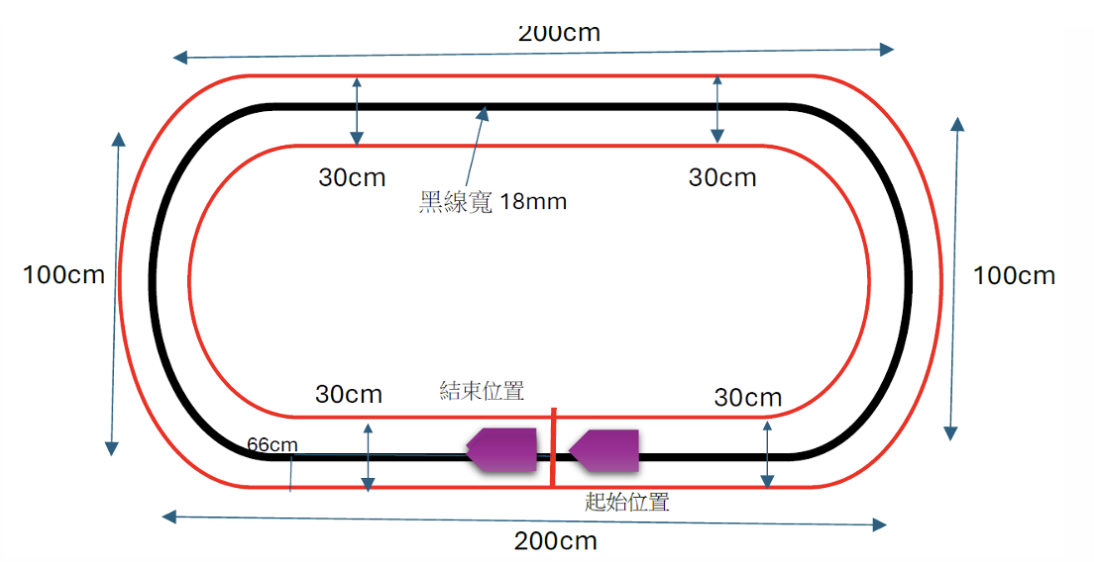
\includegraphics[width=0.7\textwidth]{1.jpg}     %圖片檔案名稱
    \caption{競賽跑道}    %圖片檔案名稱
    \label{fig:1}    %為圖片添加標籤
    %如\ref{fig:example1}所示
\end{figure}
%==============================內文==============================

\subsection{設計規範} 
%==============================內文==============================
\hspace{2em}
\begin{enumerate}
    \item 車體大小不超過A4（21.0 cm $\times$ 29.7 cm）。 
    \item 車輛僅用風力驅動，不得有其他動力來源。 
    至少3秒
    \item 扇葉需自行設計製造，且須帶有保護裝置以防扇葉 
    飛出造成傷害。 
    \item 車體載重設計須外加負載250g，模擬車手重量。 
    \item 最終總成本不得超過3000 元新台幣，且所有元件皆 
    需發票或加工證明，不可外包。 
    \item 機電系統需自行組裝與測試，可購買市售相關零組件。 
\end{enumerate}
%==============================內文==============================

\subsection{任務分工} 
%==============================內文==============================


\begin{itemize}
    \item 1100826 王子晨：演算法設計、報告撰寫
    \item 1100854 蘇威全：風扇設計、流力分析
    \item 1100862 施廷翰：車體設計、車體分析
    \item 1100812 魏羽暘：簡報製作
    \item 1100861 盧昀序：製作阿罵
\end{itemize}

%==============================內文==============================

\section{\centering 設計理念}

\subsection{車體設計} 

\subsubsection{車體結構}
%==============================內文==============================
\hspace{2em}
\begin{figure}[H]
    \centering
    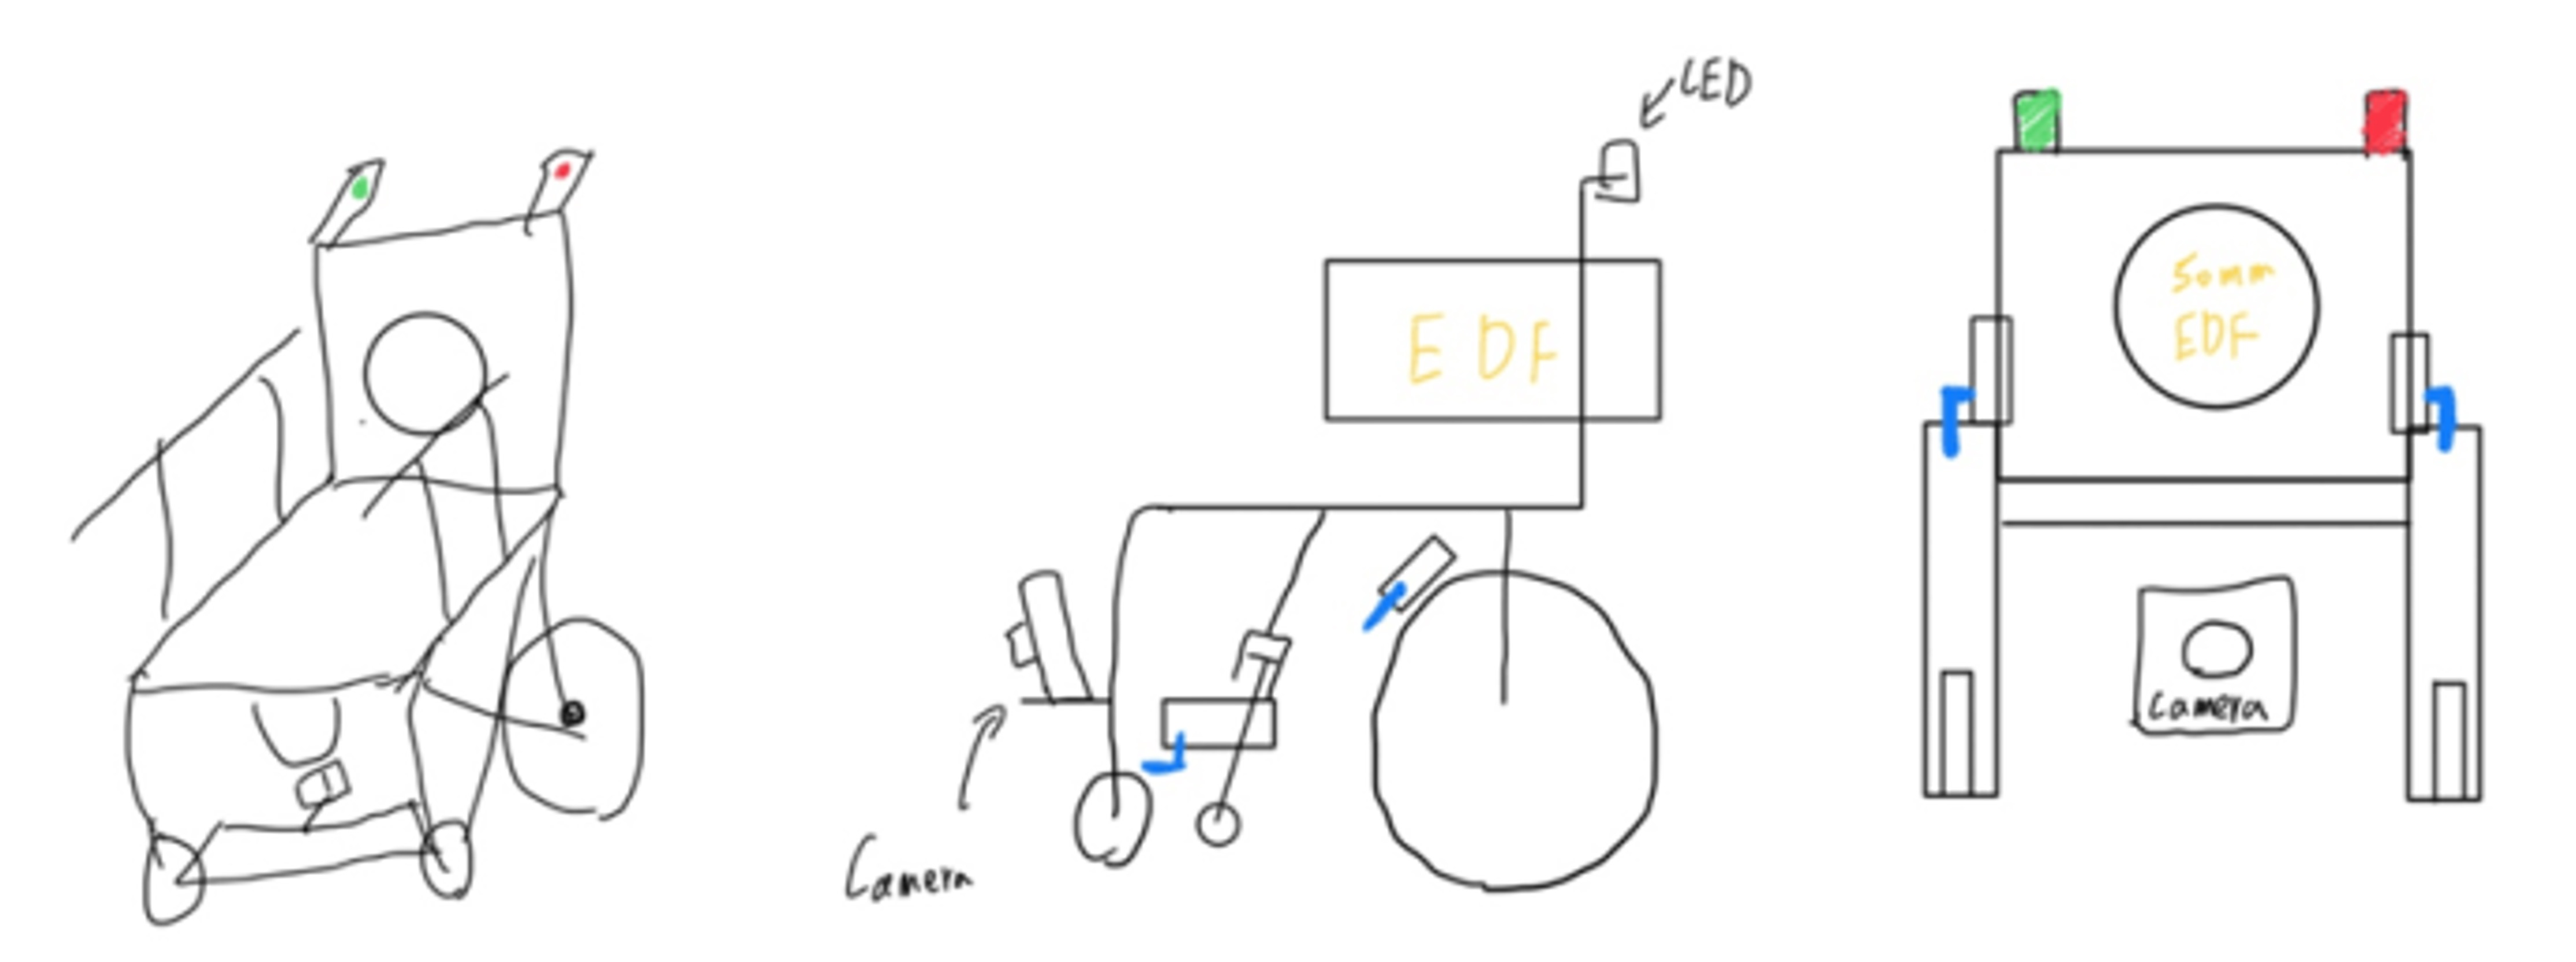
\includegraphics[width=0.7\textwidth]{2.jpg}     %圖片檔案名稱
    \caption{車體結構草圖}    %圖片檔案名稱
    \label{fig:2}    %為圖片添加標籤
    %如\ref{fig:example1}所示
\end{figure}
%==============================內文==============================

\subsubsection{影像辨識系統}
%==============================內文==============================
\hspace{2em}
\begin{figure}[H]
    \centering
    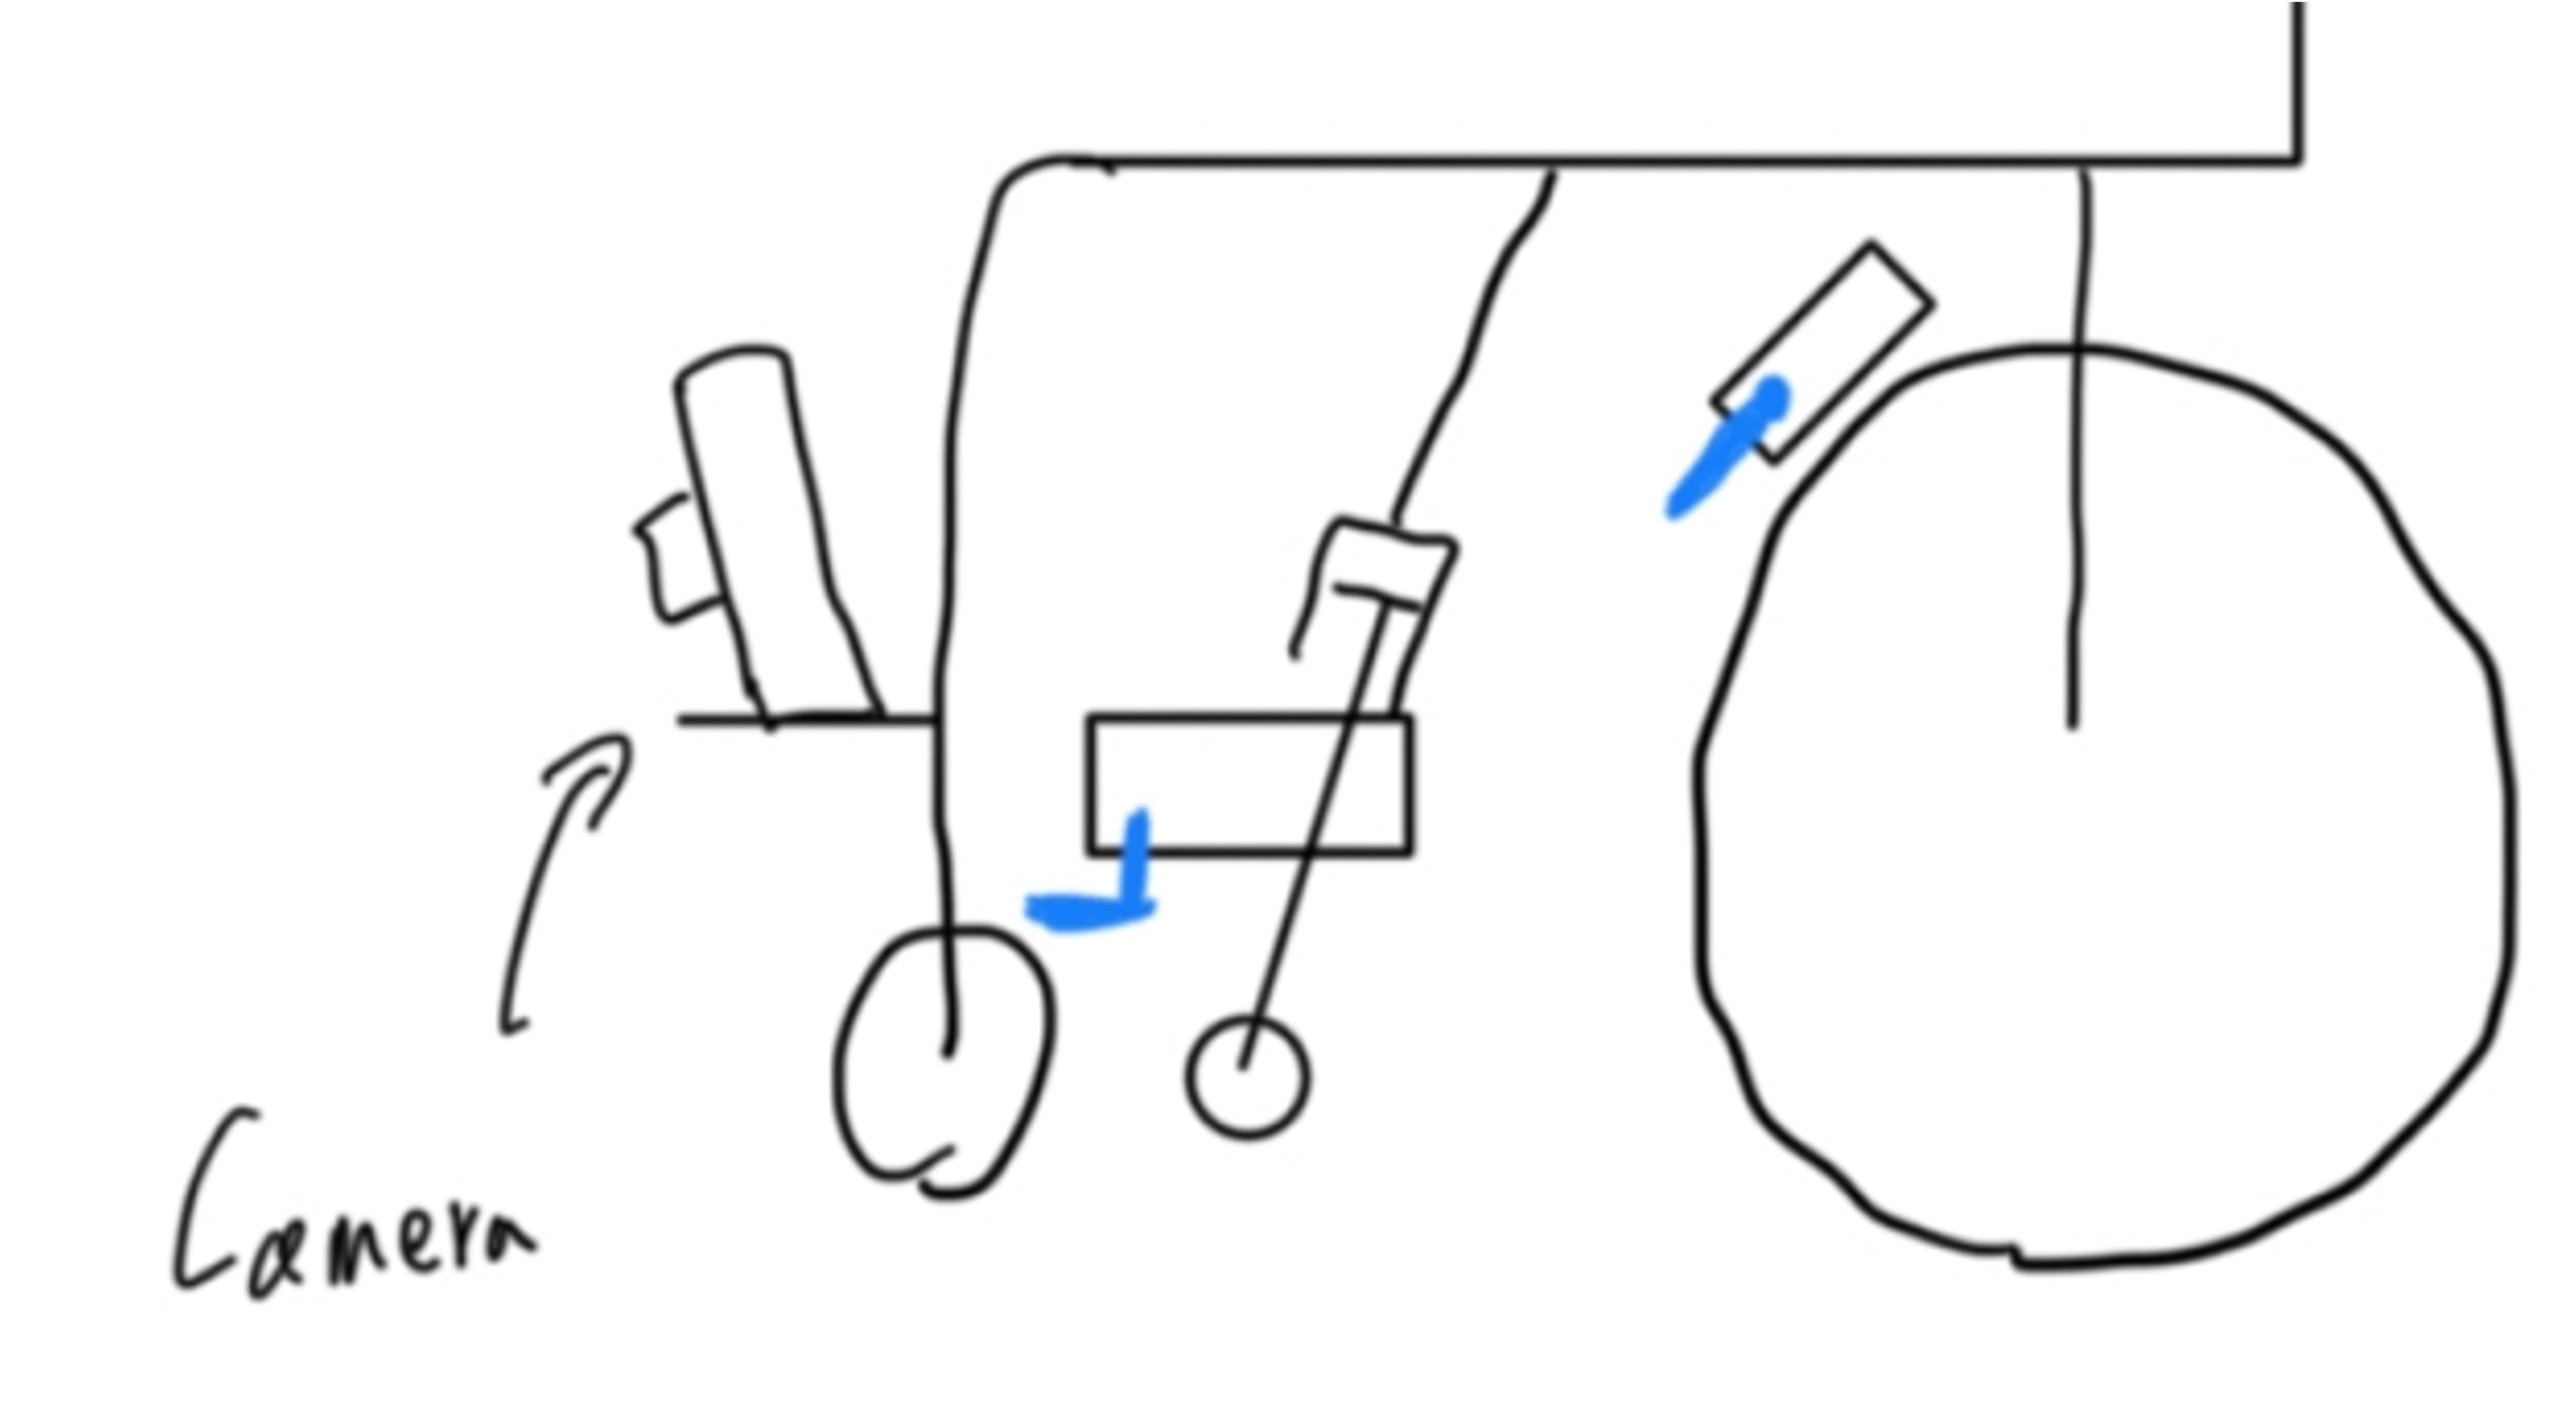
\includegraphics[width=0.7\textwidth]{3.jpg}     %圖片檔案名稱
    \caption{影像辨識系統草圖}    %圖片檔案名稱
    \label{fig:3}    %為圖片添加標籤
    %如\ref{fig:example1}所示
\end{figure}
%==============================內文==============================

\subsubsection{轉向、燈光系統}
%==============================內文==============================
\hspace{2em}
\begin{figure}[H]
    \centering
    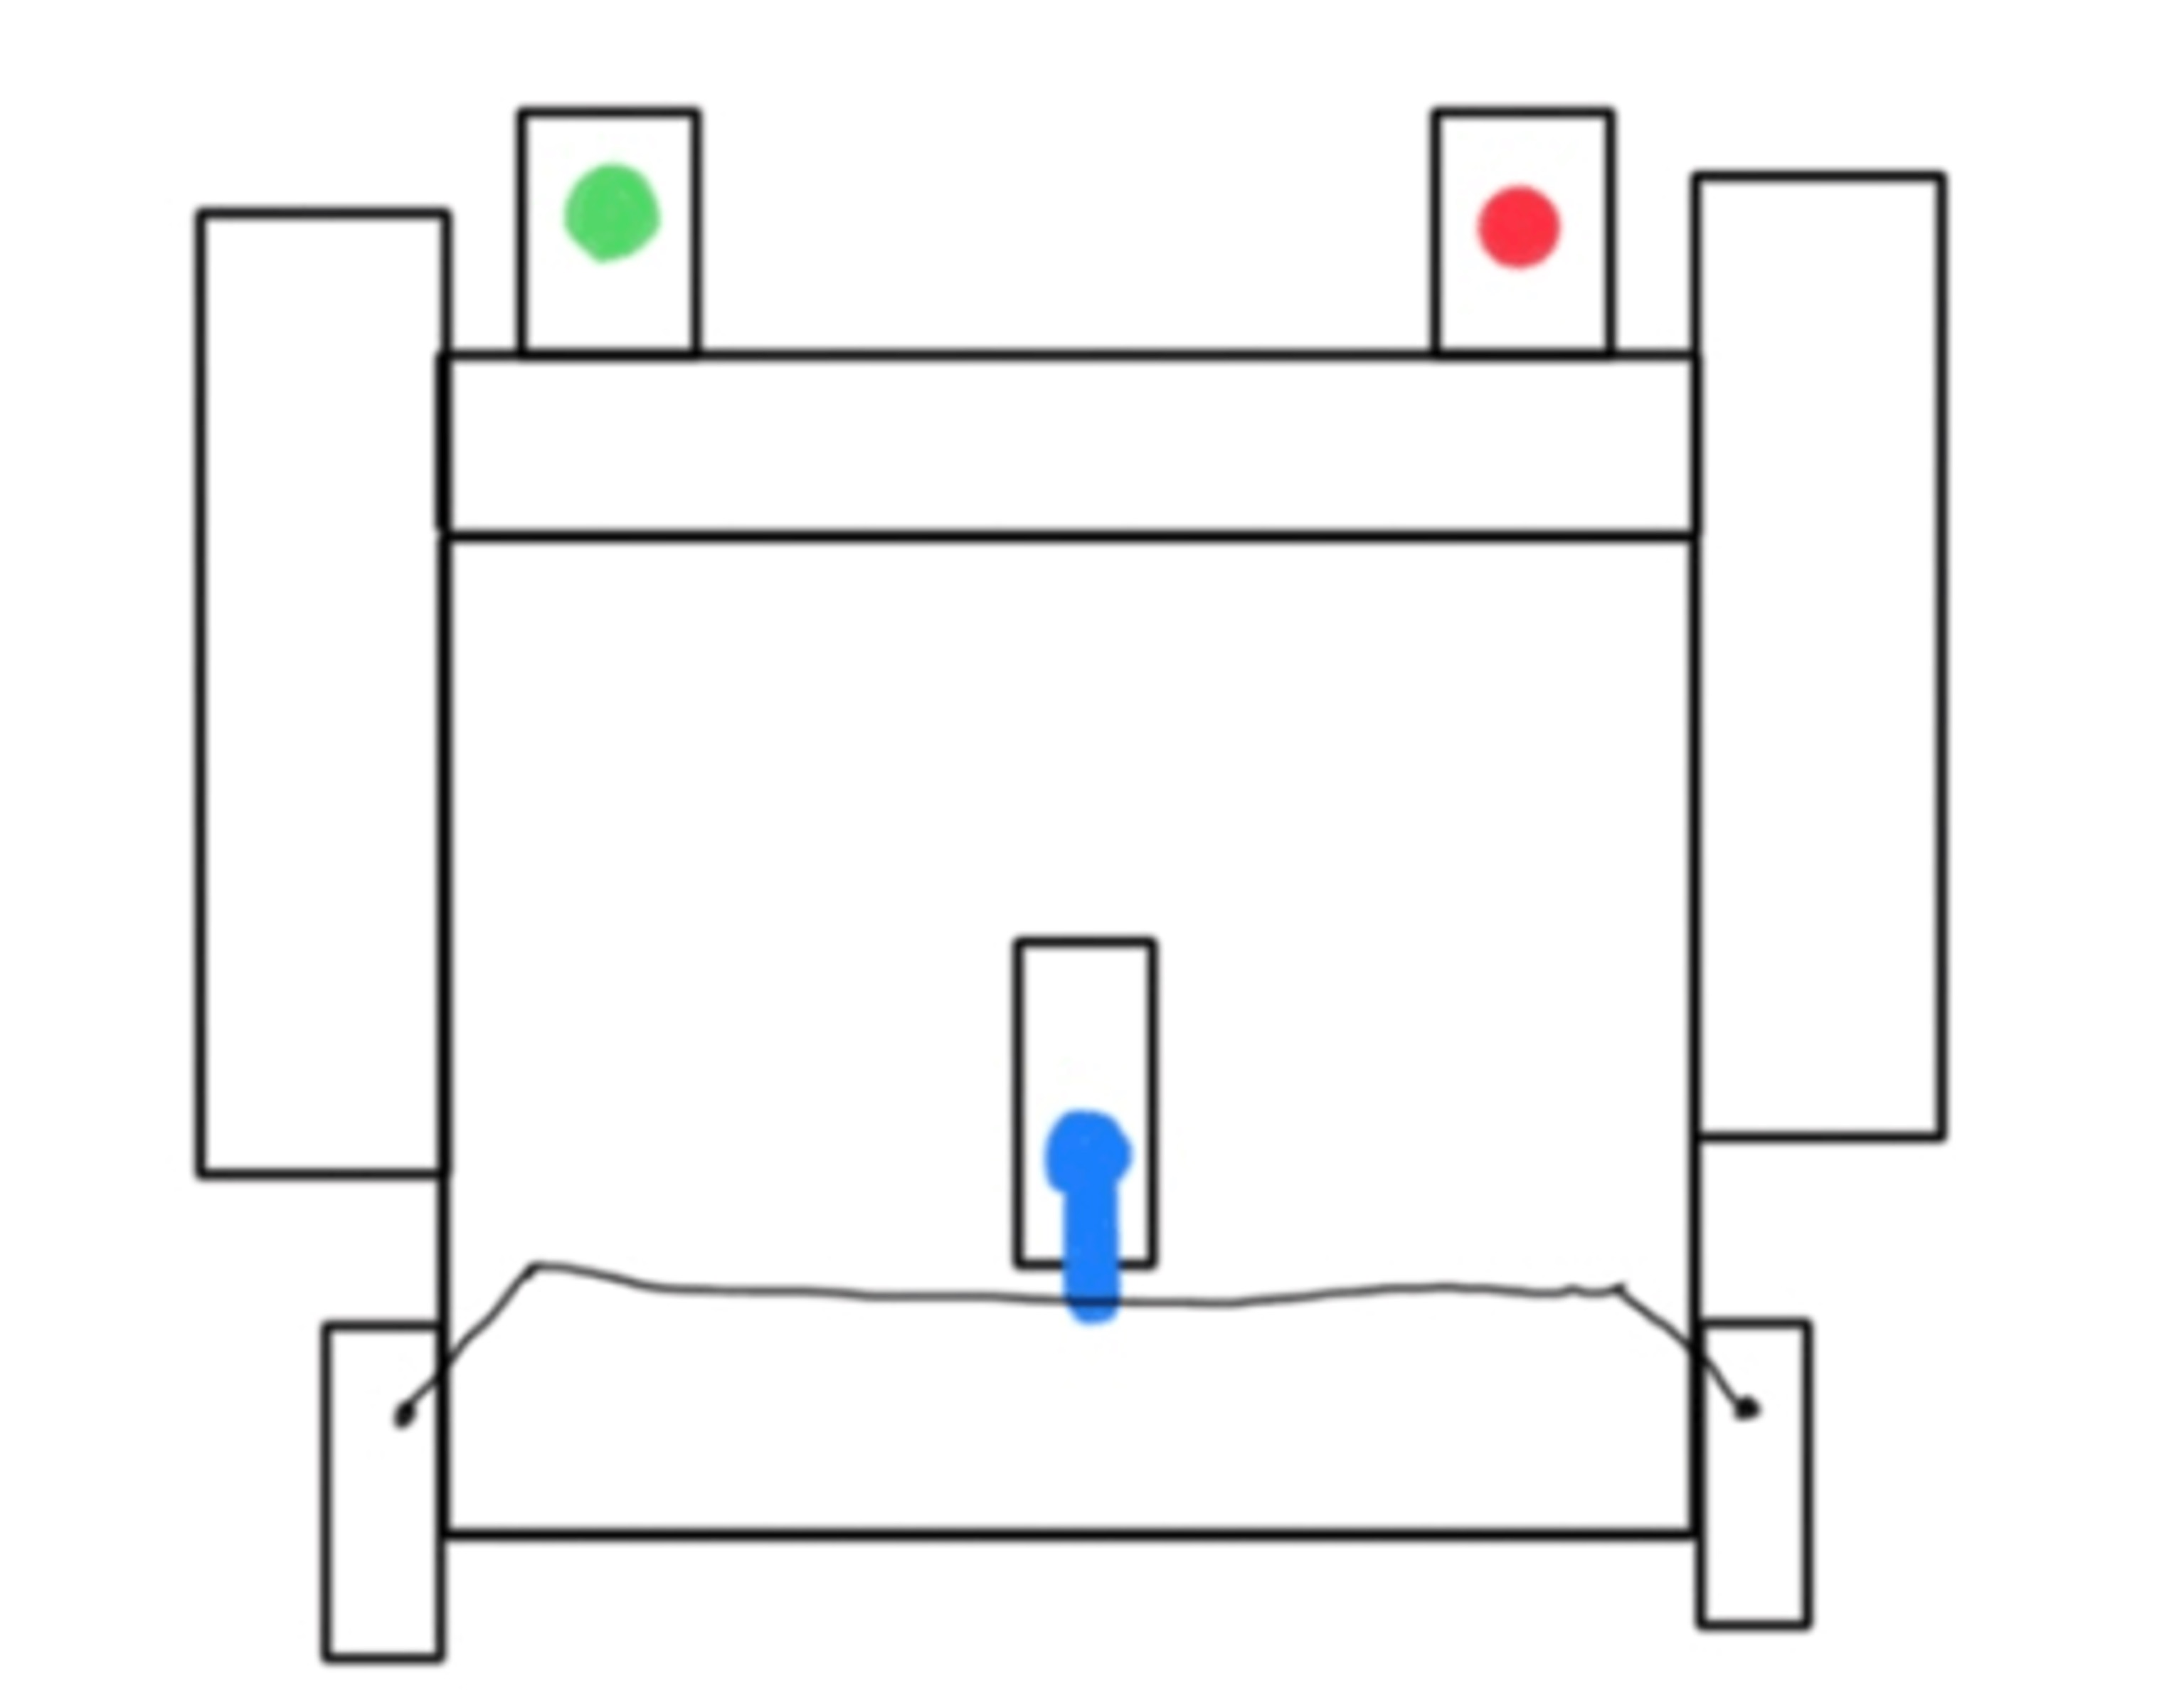
\includegraphics[width=0.7\textwidth]{4.jpg}     %圖片檔案名稱
    \caption{轉向、燈光系統草圖}    %圖片檔案名稱
    \label{fig:4}    %為圖片添加標籤
    %如\ref{fig:example1}所示
\end{figure}
%==============================內文==============================

\subsubsection{自動控制系統}
%==============================內文==============================
\hspace{2em}
\begin{figure}[H]
    \centering
    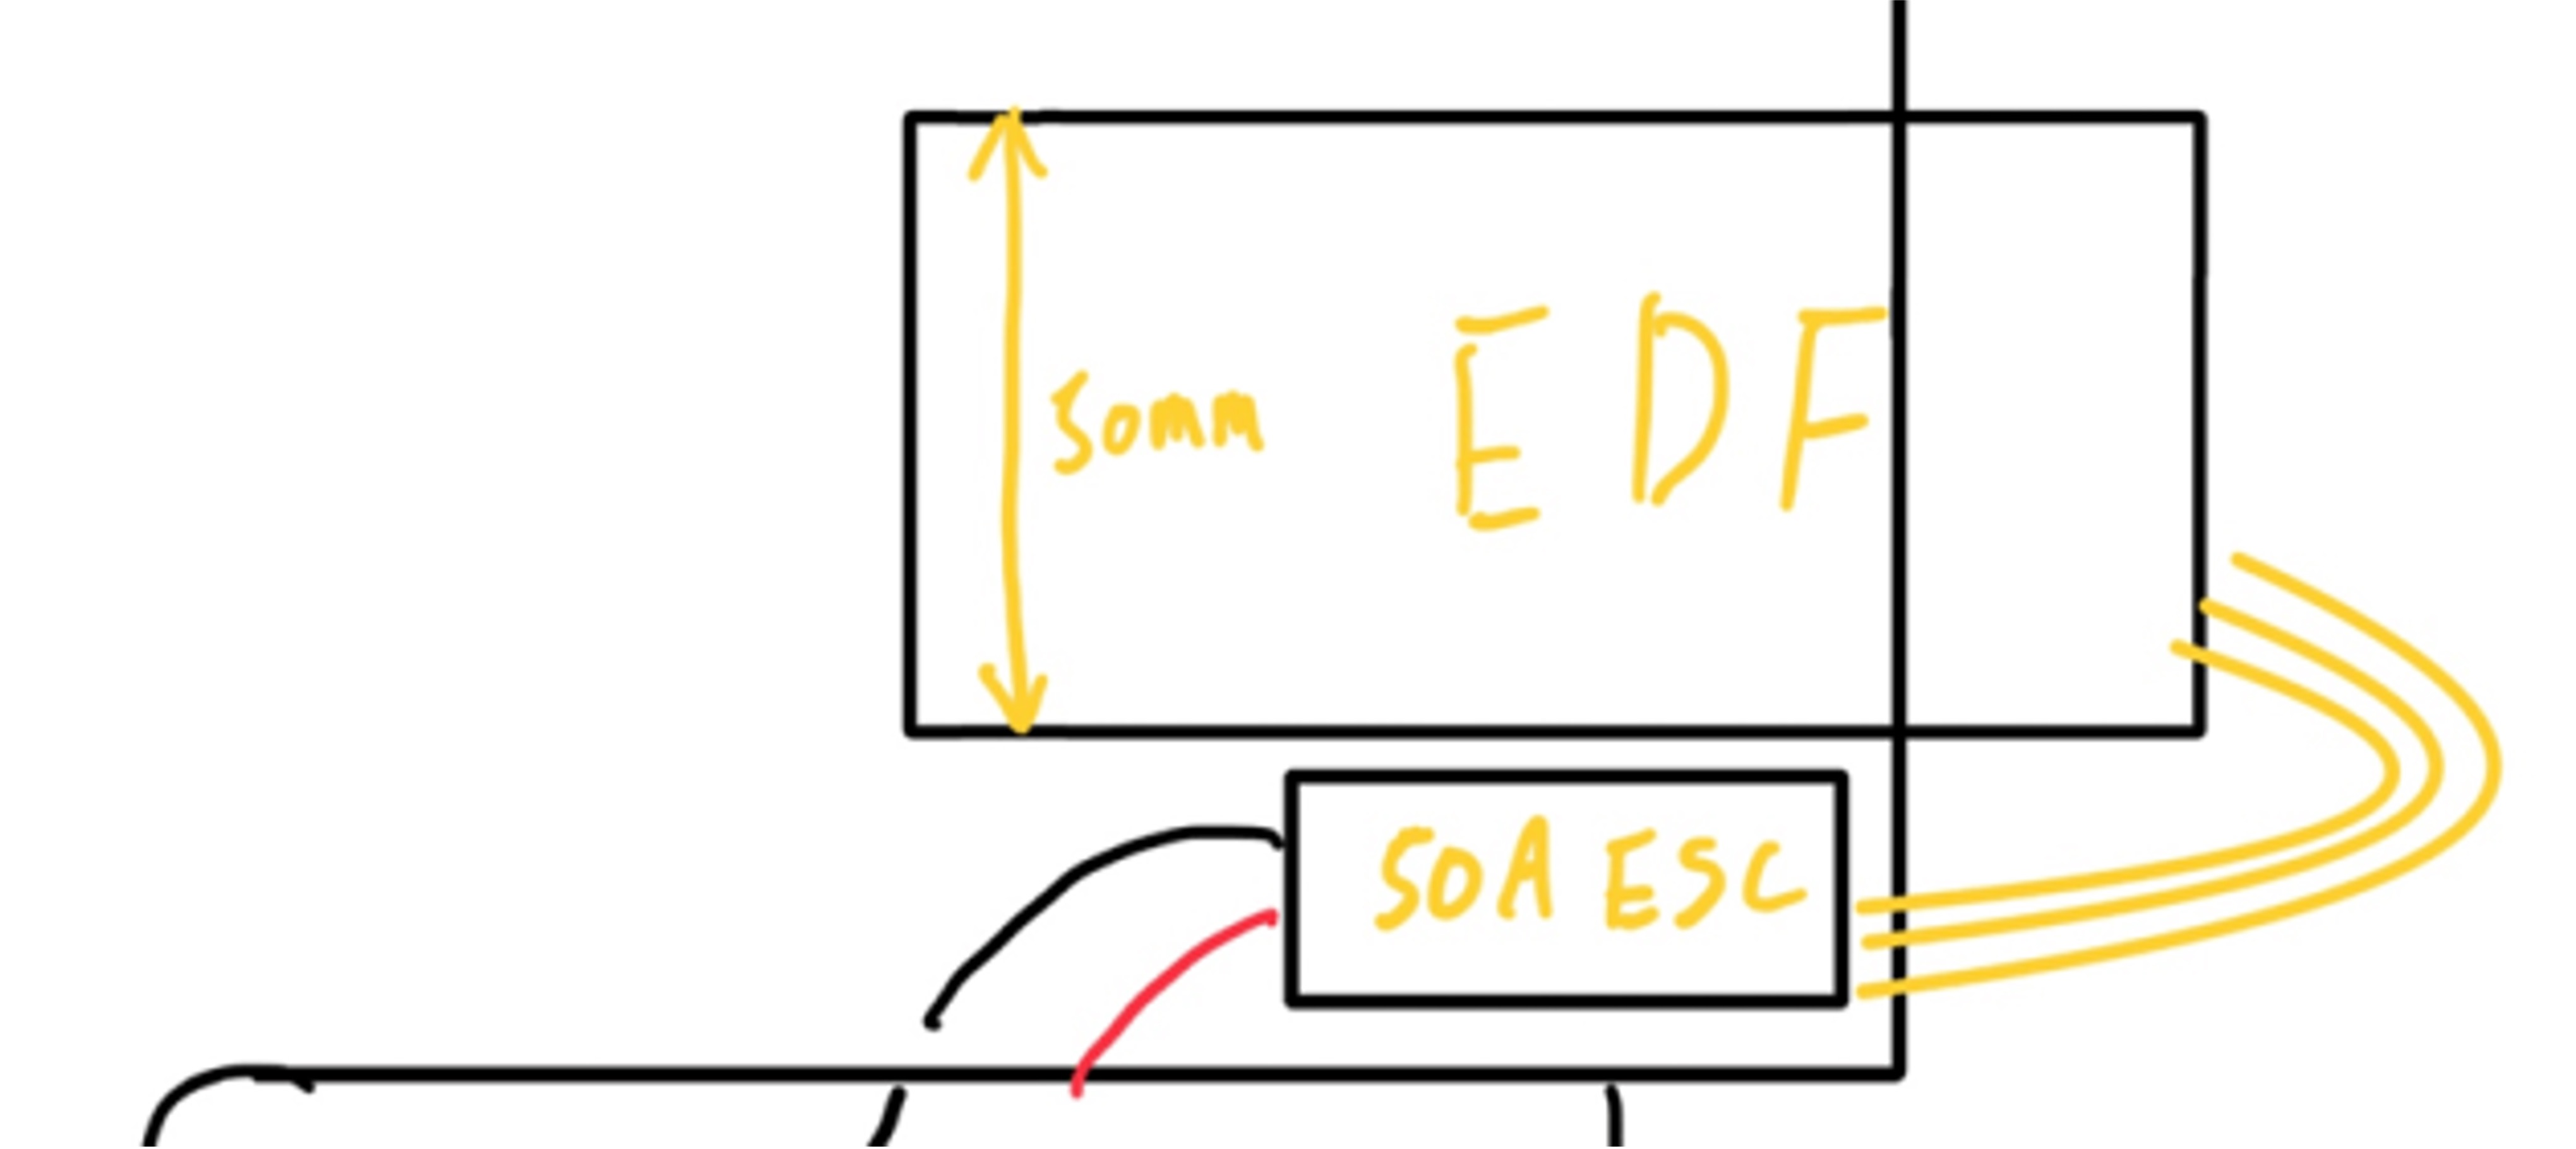
\includegraphics[width=0.7\textwidth]{5.jpg}     %圖片檔案名稱
    \caption{自動控制系統草圖}    %圖片檔案名稱
    \label{fig:5}    %為圖片添加標籤
    %如\ref{fig:example1}所示
\end{figure}
%==============================內文==============================

\subsubsection{輪椅草圖}
%==============================內文==============================
\hspace{2em}
\begin{figure}[H]
    \centering
    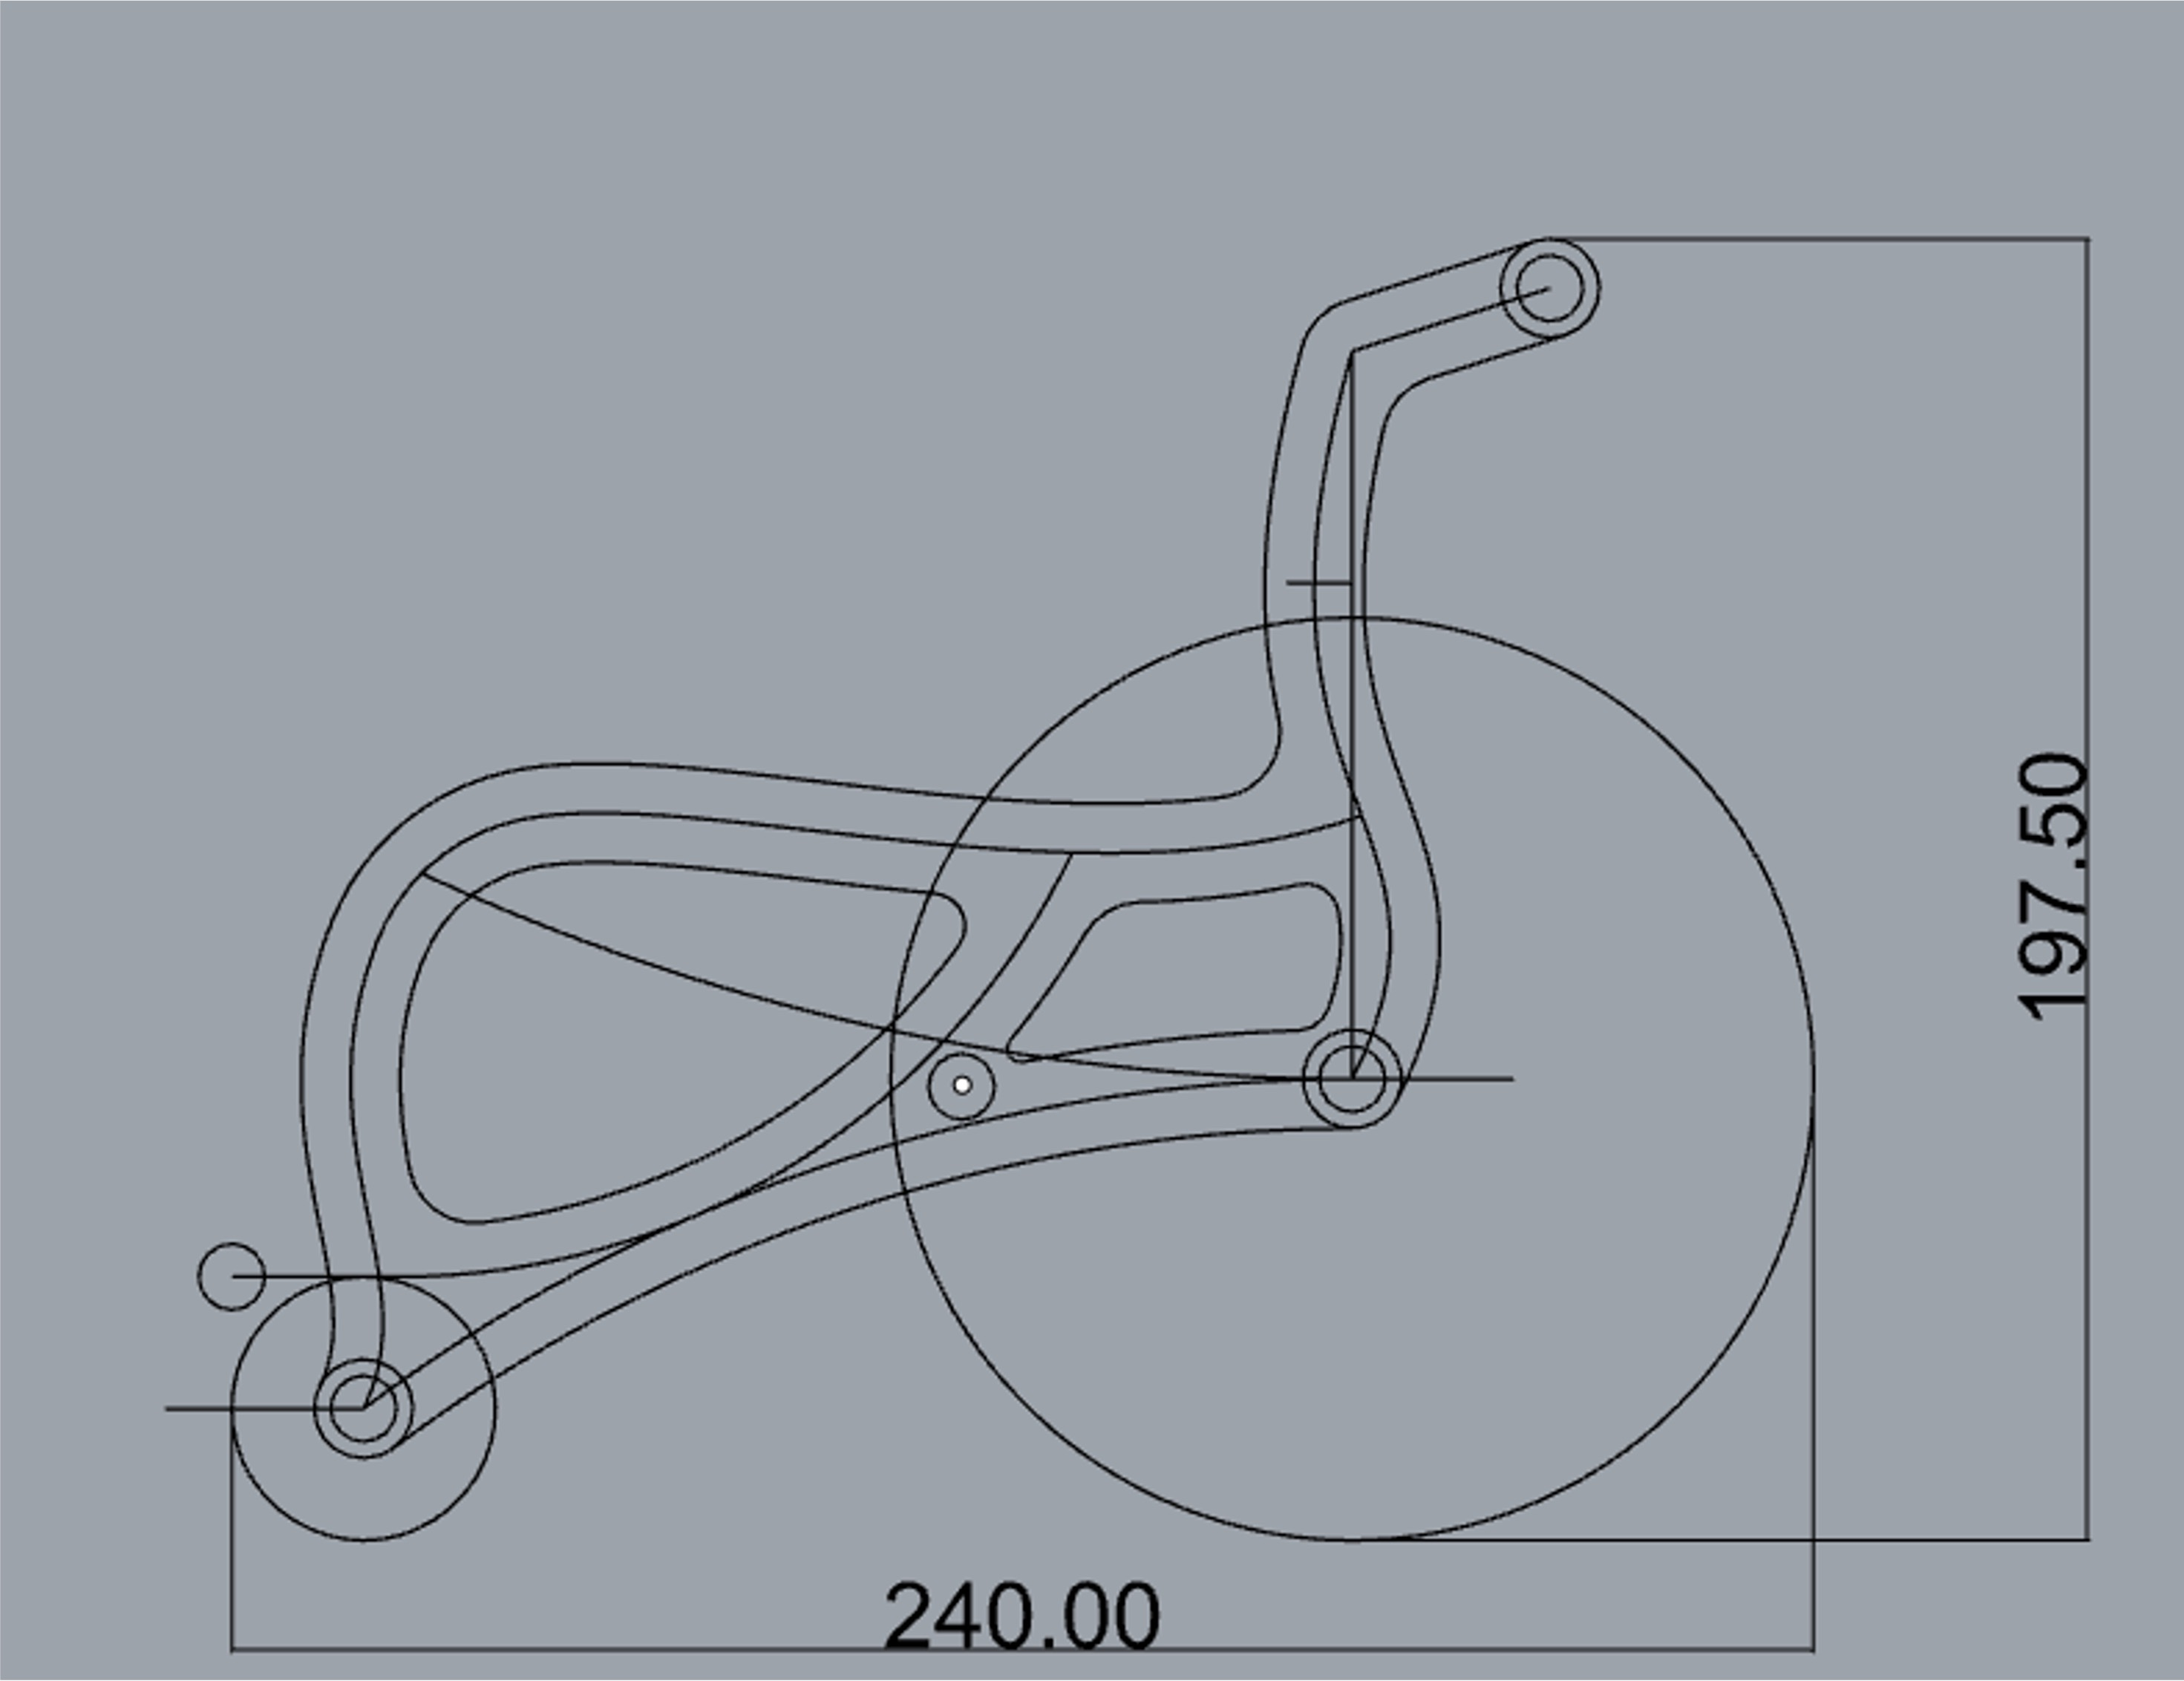
\includegraphics[width=0.6\textwidth]{6.jpg}     %圖片檔案名稱
    \caption{輪椅草圖}    %圖片檔案名稱
    \label{fig:6}    %為圖片添加標籤
    %如\ref{fig:example1}所示
\end{figure}
%==============================內文==============================

\subsubsection{硬體架構}
%==============================內文==============================
\hspace{2em}本系統以 Raspberry Pi 3B+ 作為核心控制器，負責影像處理、邏輯判斷與用戶介面等高層運算任務。考量到 Raspberry Pi 使用 3.3V TTL 電平，而 Arduino 採用 5V TTL，因此選擇透過 UART 通訊介面 進行資料交換，可有效簡化接線、降低相容性問題，並避免馬達啟停時瞬間電流對主控板造成干擾。

在系統架構中，所有感測元件（如攝影機、IMU、按鍵等）皆直接連接至 Raspberry Pi，由其統一進行資料擷取與分析；而 Arduino 則專職負責執行層控制任務，包括：
控制 EDF 風扇啟動與停止與控制伺服馬達與四連桿機構實現轉向動作。
此種分層架構不僅有助於程式模組化管理，也能提升系統穩定性與維護彈性。

\begin{figure}[H]
    \centering
    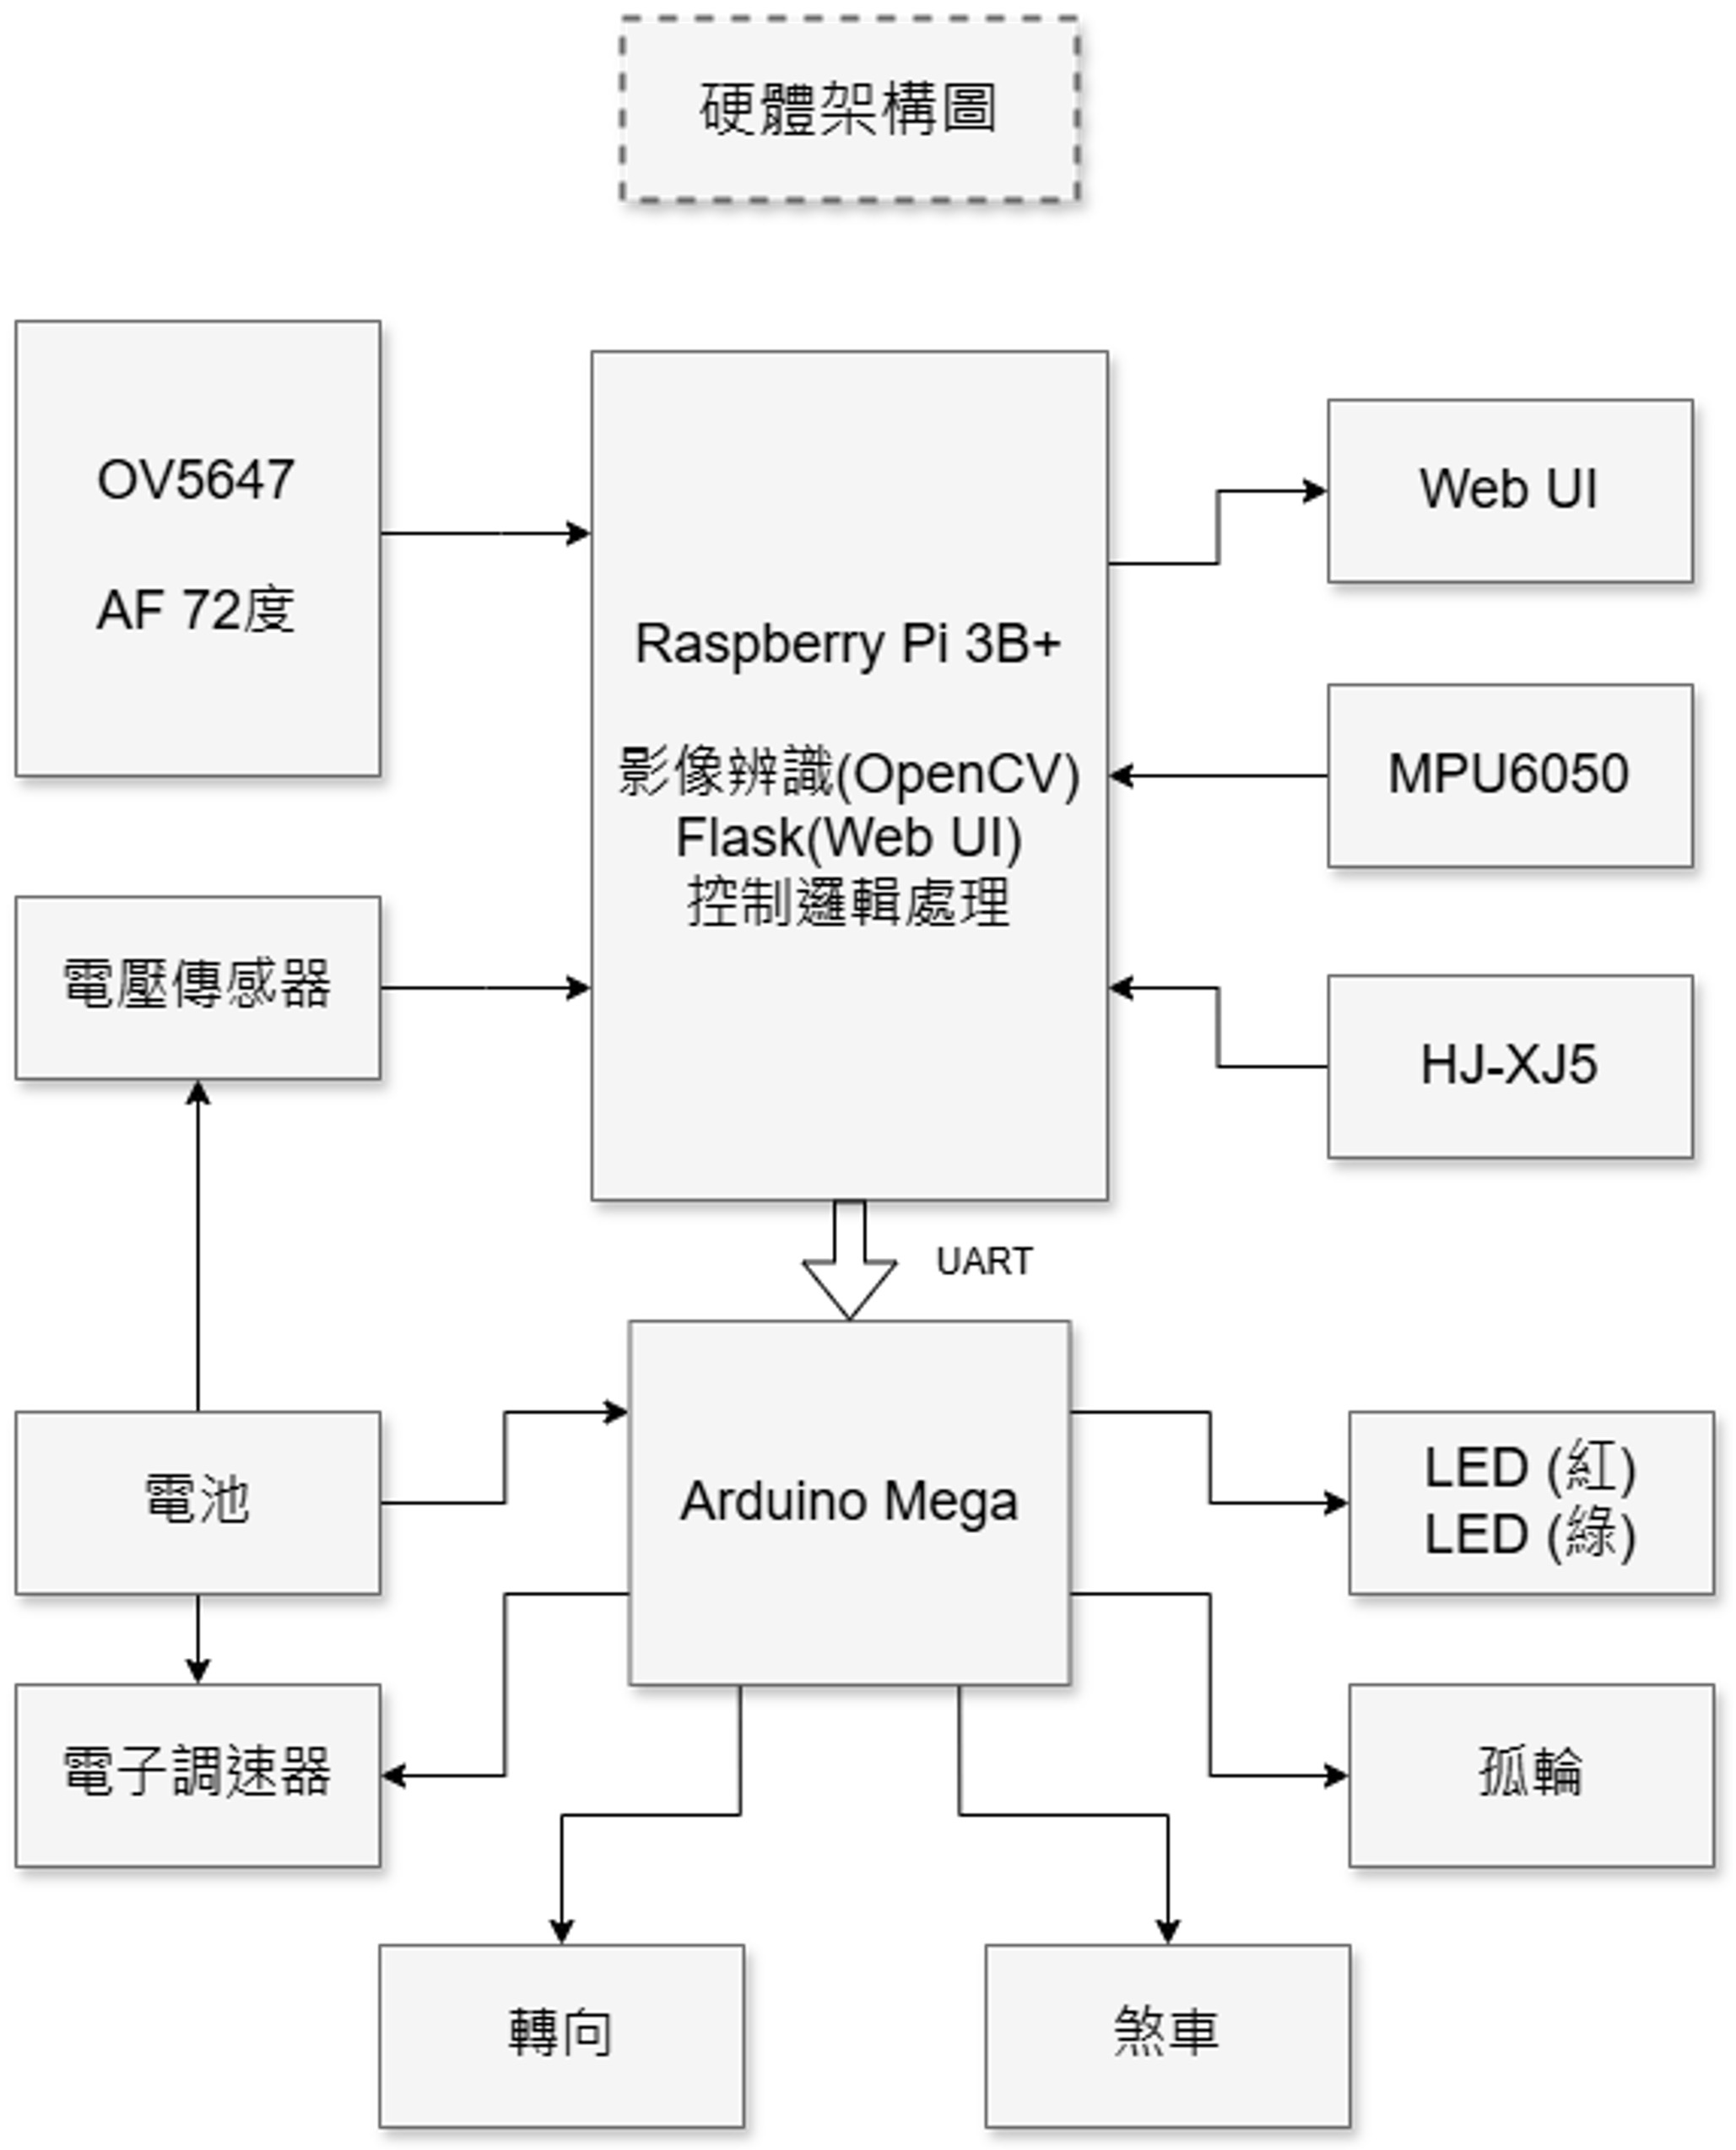
\includegraphics[width=0.6\textwidth]{7.jpg}     %圖片檔案名稱
    \caption{硬體架構圖}    %圖片檔案名稱
    \label{fig:7}    %為圖片添加標籤
    %如\ref{fig:example1}所示
\end{figure}
%==============================內文==============================
\subsection{風扇與葉片設計} 

\subsubsection{動力來源}
%==============================內文==============================
\hspace{2em}風扇通常由電動機（馬達）驅動，將電能轉換為機械能，使葉片旋轉。
%==============================內文==============================

\subsubsection{風扇設計}
%==============================內文==============================
\hspace{2em}葉片的形狀與角度（攻角）決定了風扇的效率與風量。
葉片旋轉時，根據伯努利原理與動量守恆，空氣從低壓區流向高壓區，形成風流。
葉片數量、長度與彎曲度也影響氣流模式（軸流、離心或混合流）。
%==============================內文==============================

\subsubsection{葉片設計}
%==============================內文==============================
\hspace{2em}葉片設計包含三部分，葉片數量、葉片形狀和角度、葉片長度與寬度。
葉片數量方面，少葉片（3~5片)適合高速旋轉，風速快，但風壓較低。多葉片（7片以上)：提供較高的風壓，適合對抗阻力的應用（如散熱器、空調）。

葉片形狀與角度這方面葉片的攻角（Blade Angle)影響空氣推動力。較大攻角（20~45°)提供較高風壓，但阻力增加，可能降低轉速。較小攻角（10~20°)提升風速，適合低阻力環境。
扭曲葉片，可減少渦流，提高效率。仿生學設計(如模仿鯨魚胸鰭、鷹翼)可減少空氣阻力，提高流動效率。

葉片長度與寬度方面加長葉片可提高風量，但需注意馬達負載。加寬葉片有助於提升風壓，適用於高阻力場景。

我們的設計策略是根據應用需求選擇葉片數量，確保風壓與風量的平衡。
%==============================內文==============================

\subsection{電機與轉速} 
%==============================內文==============================
\hspace{2em}風力大小與轉速成正比需選擇高效能電機，如：無刷直流電機（BLDC)：效率高、壽命長，適合高速風扇。感應電機（Induction Motor)：適用於大功率風扇。

我們使用的風扇規格如表\ref{tab:fan}所示：
    \begin{table}[H]
        \centering
        \caption{風扇規格}
        \vspace{6pt} % 增加空格
        \label{tab:fan}
        \begin{tabular}{ll}
            \toprule
            \textbf{項目} & \textbf{規格} \\
            \midrule
            風扇直徑 \(D\) & \(50\,\mathrm{mm} = 0.05\,\mathrm{m}\) \\
            葉片數 & 11 \\
            EDF 型號 & \(50\,\mathrm{mm}\,EDF\) \\
            馬達 KV 值 & \(4500\,\mathrm{KV}\)\\
            電池電壓 & \(3S = 11.1\,\mathrm{V}\)\\
            \bottomrule
        \end{tabular}
        %如\ref{tab:TT2}所示
    \end{table}

    理論轉速計算如下：
    \begin{align}
        \text{RPM} &= KV \times V = 4500 \times 11.1  \label{eq:1}
        \\
        &= 49950\text{RPM} \nonumber
        %式\ref{eq:2}
    \end{align}

    風扇出口速度計算式\ref{eq:2}，$V_e$為出口速度，$\text{RPM}$為馬達轉速，$\text{D}$為風扇直徑，$K_e$為出口速度係數(通常介於0.1至0.2)。
    \begin{align}
        V_e &= K_e \cdot \text{RPM} \cdot D  \label{eq:2}
        \\
        &= 0.1 \cdot 49950 \cdot 0.05  \nonumber
        \\
        &= 249.75 m/s \nonumber
        %式\ref{eq:2}
    \end{align}
%==============================內文==============================

\subsection{風道與結構設計} 
\subsubsection{風扇外框與導流設計}
%==============================內文==============================
\begin{itemize}
    \item 加裝導風罩(Shroud)可集中氣流，提高風速與效率。
    \item 收縮式進風口(如噴嘴設計)可增加流速，提高出風動能。
    \item 擾流板(Guide Vanes)可減少渦流，提升氣流穩定度。
\end{itemize}
%==============================內文==============================

\subsubsection{風扇類型選擇}
%==============================內文==============================
\begin{itemize}
    \item 軸流風扇(Axial Fan)適合長距離送風(如電腦散熱、風扇塔)。
    \item 離心風扇(Centrifugal Fan)適合高風壓應用(如空調、渦輪增壓器)。

    \item 混流風扇(Mixed Flow Fan)結合兩者優勢，提高風壓與風量。
\end{itemize}
%==============================內文==============================

\subsubsection{風扇導流罩}
%==============================內文==============================
\hspace{2em}主要作用是提升風扇的推力與效率，其原理涉及氣流控制、減少渦流、提高風壓與風速。
導流罩的幾個關鍵機制為增加氣流速度(噴射效應)與減少渦流與能量損失。
風扇在運轉時，葉片末端(特別是無外框的風扇)會產生強烈的端部渦流(Tip Vortex)會導致氣流擾動降低風壓與能量損耗使推力下降。

導流罩可封閉葉片端部，減少氣流洩漏，進而提高風扇效率。目前打算設計變截面導流罩(Converging Nozzle)，入口與出口皆有變化，可提升氣流效率，減少能量損耗。
%==============================內文==============================

\subsection{空氣動力學設計} 
%==============================內文==============================
\begin{itemize}
    \item 降低車身阻力(Drag Reduction)
    \item 流線型設計，避免平直表面，減少風阻
    \item 使用導流罩(Shroud)引導風扇氣流，提高推進效率
    \item 穩定性
    \item 風扇的反作用力可能影響車輛平衡，需要考慮重心設計
    \item 若車輛速度高，可加裝尾翼，減少側風影響
\end{itemize}

推力計算如下所示，$\rho = 1.225(kg/m^3)$、$V_i =0$、$D=0.05(m)$：
\begin{align}
    T &= \dot{m} \cdot (V_e - V_i) \label{eq:thrust_formula} 
    \\
    &= \rho \cdot A \cdot V_e \cdot (V_e - V_i)   \nonumber
    \\
    &= \rho \cdot \frac{1}{4} \cdot D^2\cdot \pi \cdot V_e \cdot (V_e - V_i)   \nonumber
    \\
     &=1.225\times \frac{\pi}{4}\times 0.05^2 \times249.75\times(249.75-0) \nonumber
    \\
    T &= 150.0296(N)    \nonumber
\end{align}

當汽車行駛時，會受到空氣阻力，$CD$為阻力係數，$\rho$為空氣密度，$A$車體迎風面，$v$為車速，其公式如式\ref{eq:3}。
\begin{align}
    FD=\frac{1}{2}CDv^{2}\rho A  \label{eq:3}
    %式\ref{eq:2}
\end{align}
降低空氣阻力的方法包含流線型車身設計（減少迎風面積）、降低車輛高度（減少底部亂流）、使用導流板（減少渦流與尾流）。

汽車在高速行駛時，車身可能會產生升力(Lift)，導致車輛不穩定而F1賽車則透過空氣動力學產生下壓力(Downforce)來增加抓地力。升力公式如式\ref{eq:3}。
\begin{align}
    FL=\frac{1}{2}CLv^{2}\rho A  \label{eq:4}
    %式\ref{eq:2}
\end{align}
減少升力的方法包含加裝尾翼（Spoiler）、底部擴散器（Diffuser）、前擾流板（Front Splitter）。
加裝尾翼可改變氣流方向，增加下壓力。底部擴散器，增加地面效應，減少氣流擾動。前擾流板可提升車頭穩定性。

風扇驅動車是靠風扇推進，需要考慮：

\begin{enumerate}
    \item 風扇的推力與效率 : 使用導流(Shroud)來提高推力。
    \item 車身形狀 : 流線型設計可減少阻力，讓風扇推動更有效。
    \item 尾流管理 : 避免車後氣流分離，降低拖曳力，提高速度。
\end{enumerate}
%==============================內文==============================

\subsection{演算法設計} 
%==============================內文==============================
\hspace{2em}循線演算法將結合影像偵測與模糊控制實現，並包含預處理、偵測、模糊控制三部分。演算法流程圖如\ref{fig:9}圖所示。
\begin{figure}[H]
    \centering
    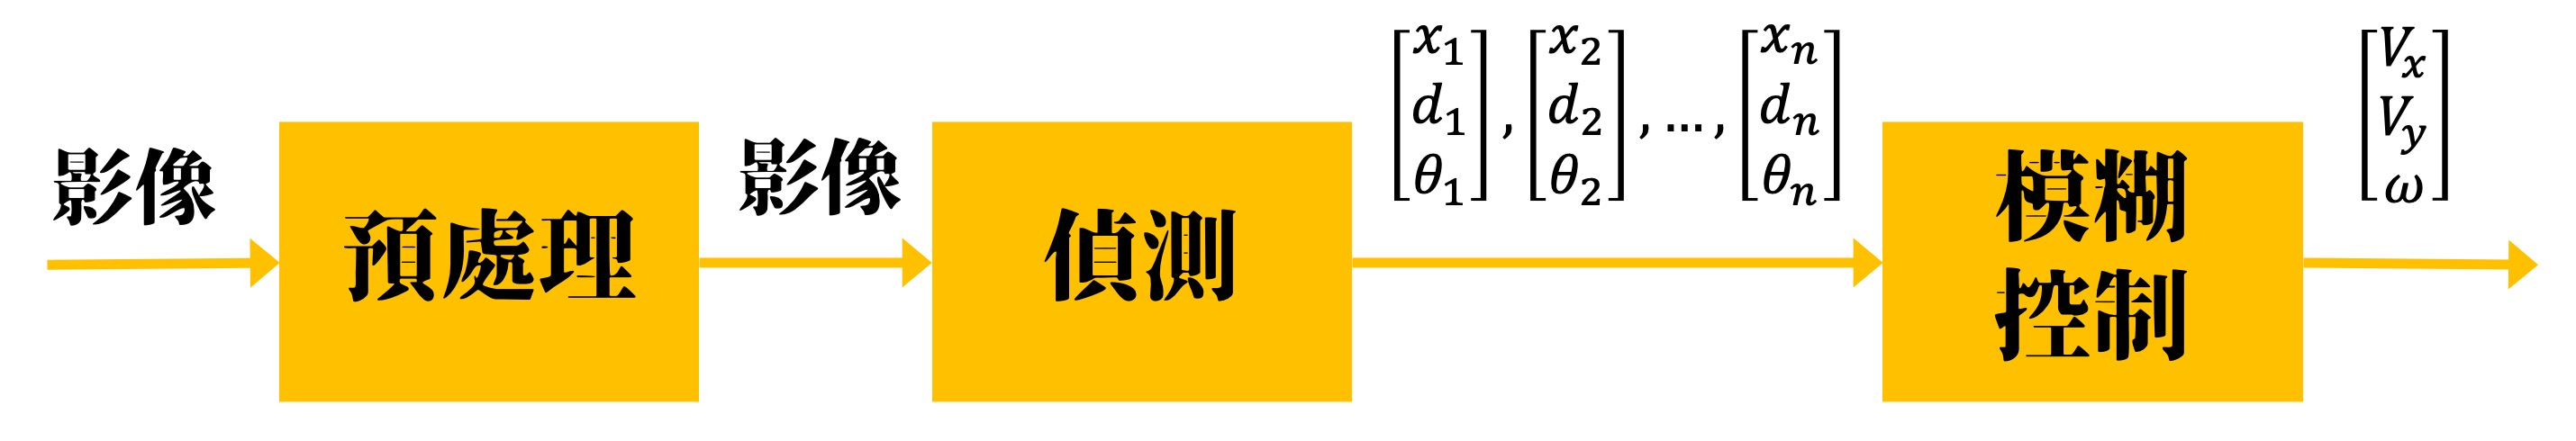
\includegraphics[width=0.9\textwidth]{9.jpg}     %圖片檔案名稱
    \caption{影像循線演算法流程圖}    %圖片檔案名稱
    \label{fig:9}    %為圖片添加標籤
    %如\ref{fig:example1}所示
\end{figure}

演算法的輸入為影像，演算法的輸出為車輛為$V_{x}$、$V_{y}$與$\omega$，定義如下圖\ref{fig:10}所示。
\begin{figure}[H]
    \centering
    
\includegraphics[width=0.5\textwidth]{10.jpg}     %圖片檔案名稱
    \caption{車輛速度定義}    %圖片檔案名稱
    \label{fig:10}    %為圖片添加標籤
    %如\ref{fig:example1}所示
\end{figure}
%==============================內文==============================

\subsubsection{預處理}
%==============================內文==============================
\hspace{2em} 此部分要將影像拍攝影像處理成可供影像偵測之影像，包括透視變換、灰階處理、高斯模糊、二值化、Canny邊緣偵測五步驟，將接收到的影像進行處理，提供後續偵測使用。

\begin{figure}[H]
    \centering
    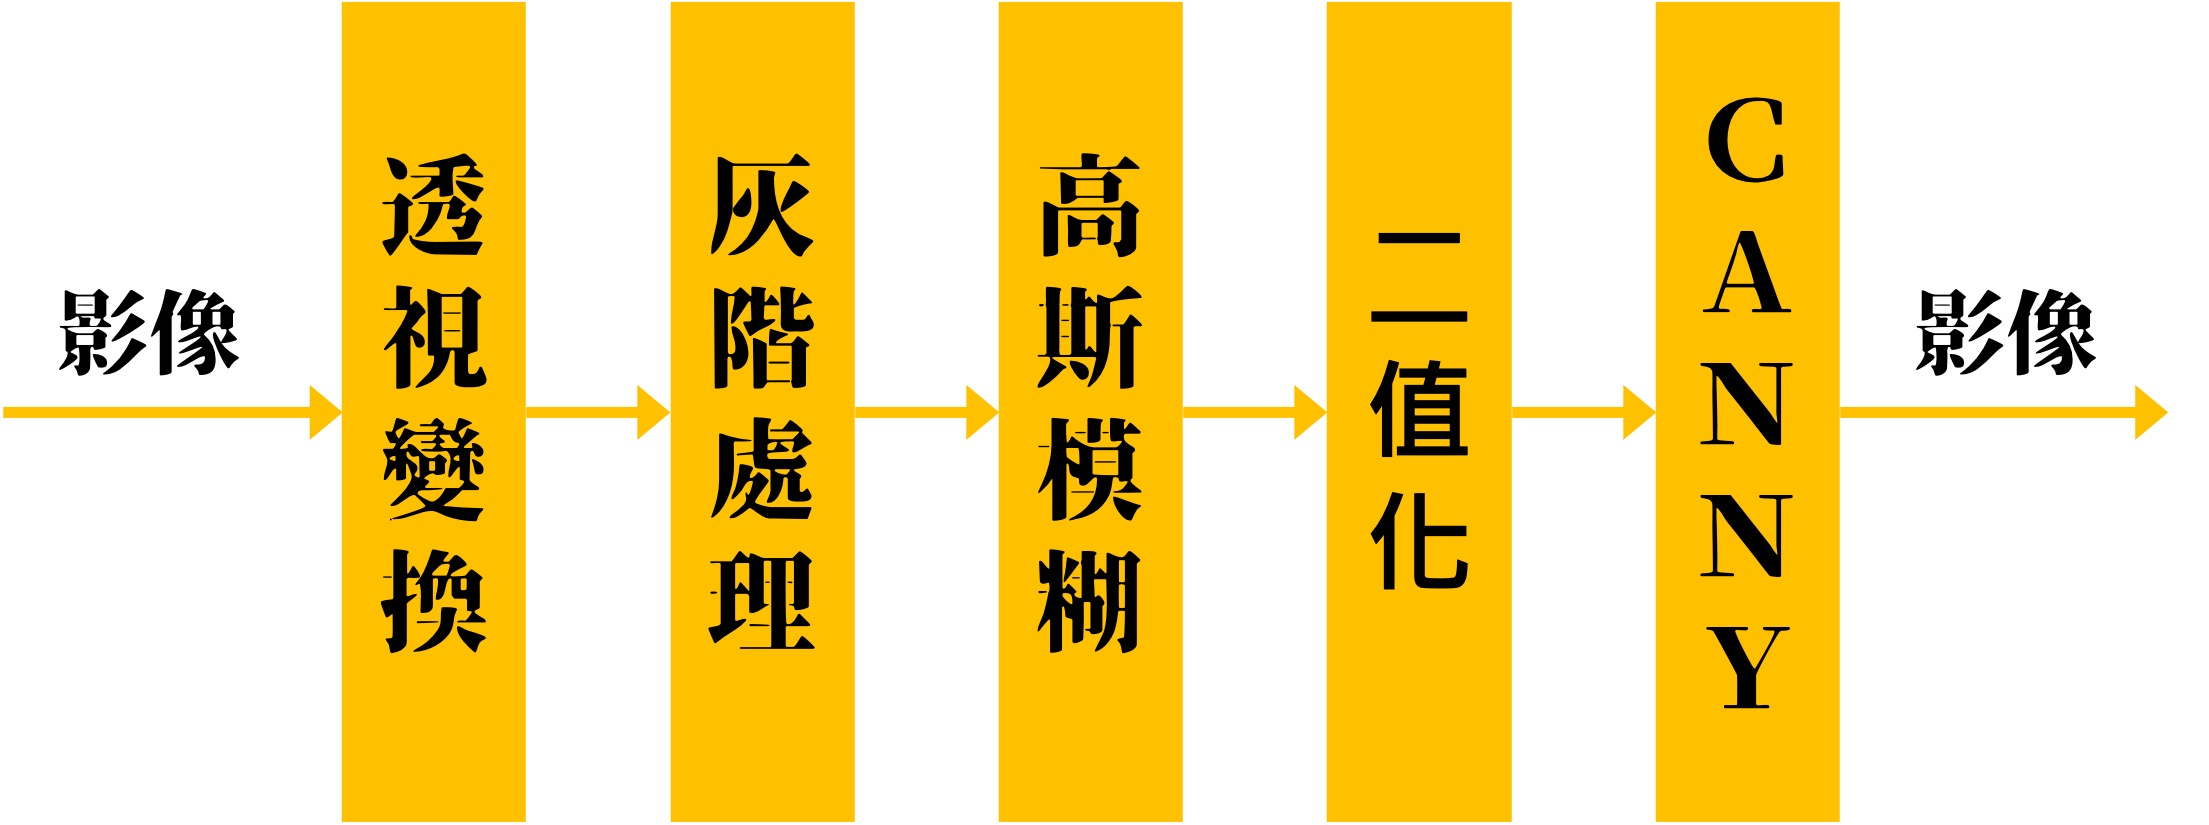
\includegraphics[width=0.7\textwidth]{11.jpg}     %圖片檔案名稱
    \caption{影像預處理流程圖}    %圖片檔案名稱
    \label{fig:11}    %為圖片添加標籤
    %如\ref{fig:example1}所示
\end{figure}

首先，對捕獲的影像進行透視變換，將影像轉換為以車輛為原點的二維座標系統，這樣有助於確定車輛與道路的相對位置，並為後續的計算提供準確的基準。公式\ref{eq:fy}及示意圖(如圖\ref{fig:15}、圖\ref{fig:14}所示)如下：
\begin{align}
    \begin{bmatrix}
        x_{car}   \\
        y_{car}   
    \end{bmatrix} 
     &=f(
     \begin{bmatrix}
        x       \\
        y       
    \end{bmatrix} 
    ,W,H,\theta_{camera},HFOV,WFOV)
    \label{eq:xcarycar}
\end{align}
\begin{figure}[H]
    \centering
    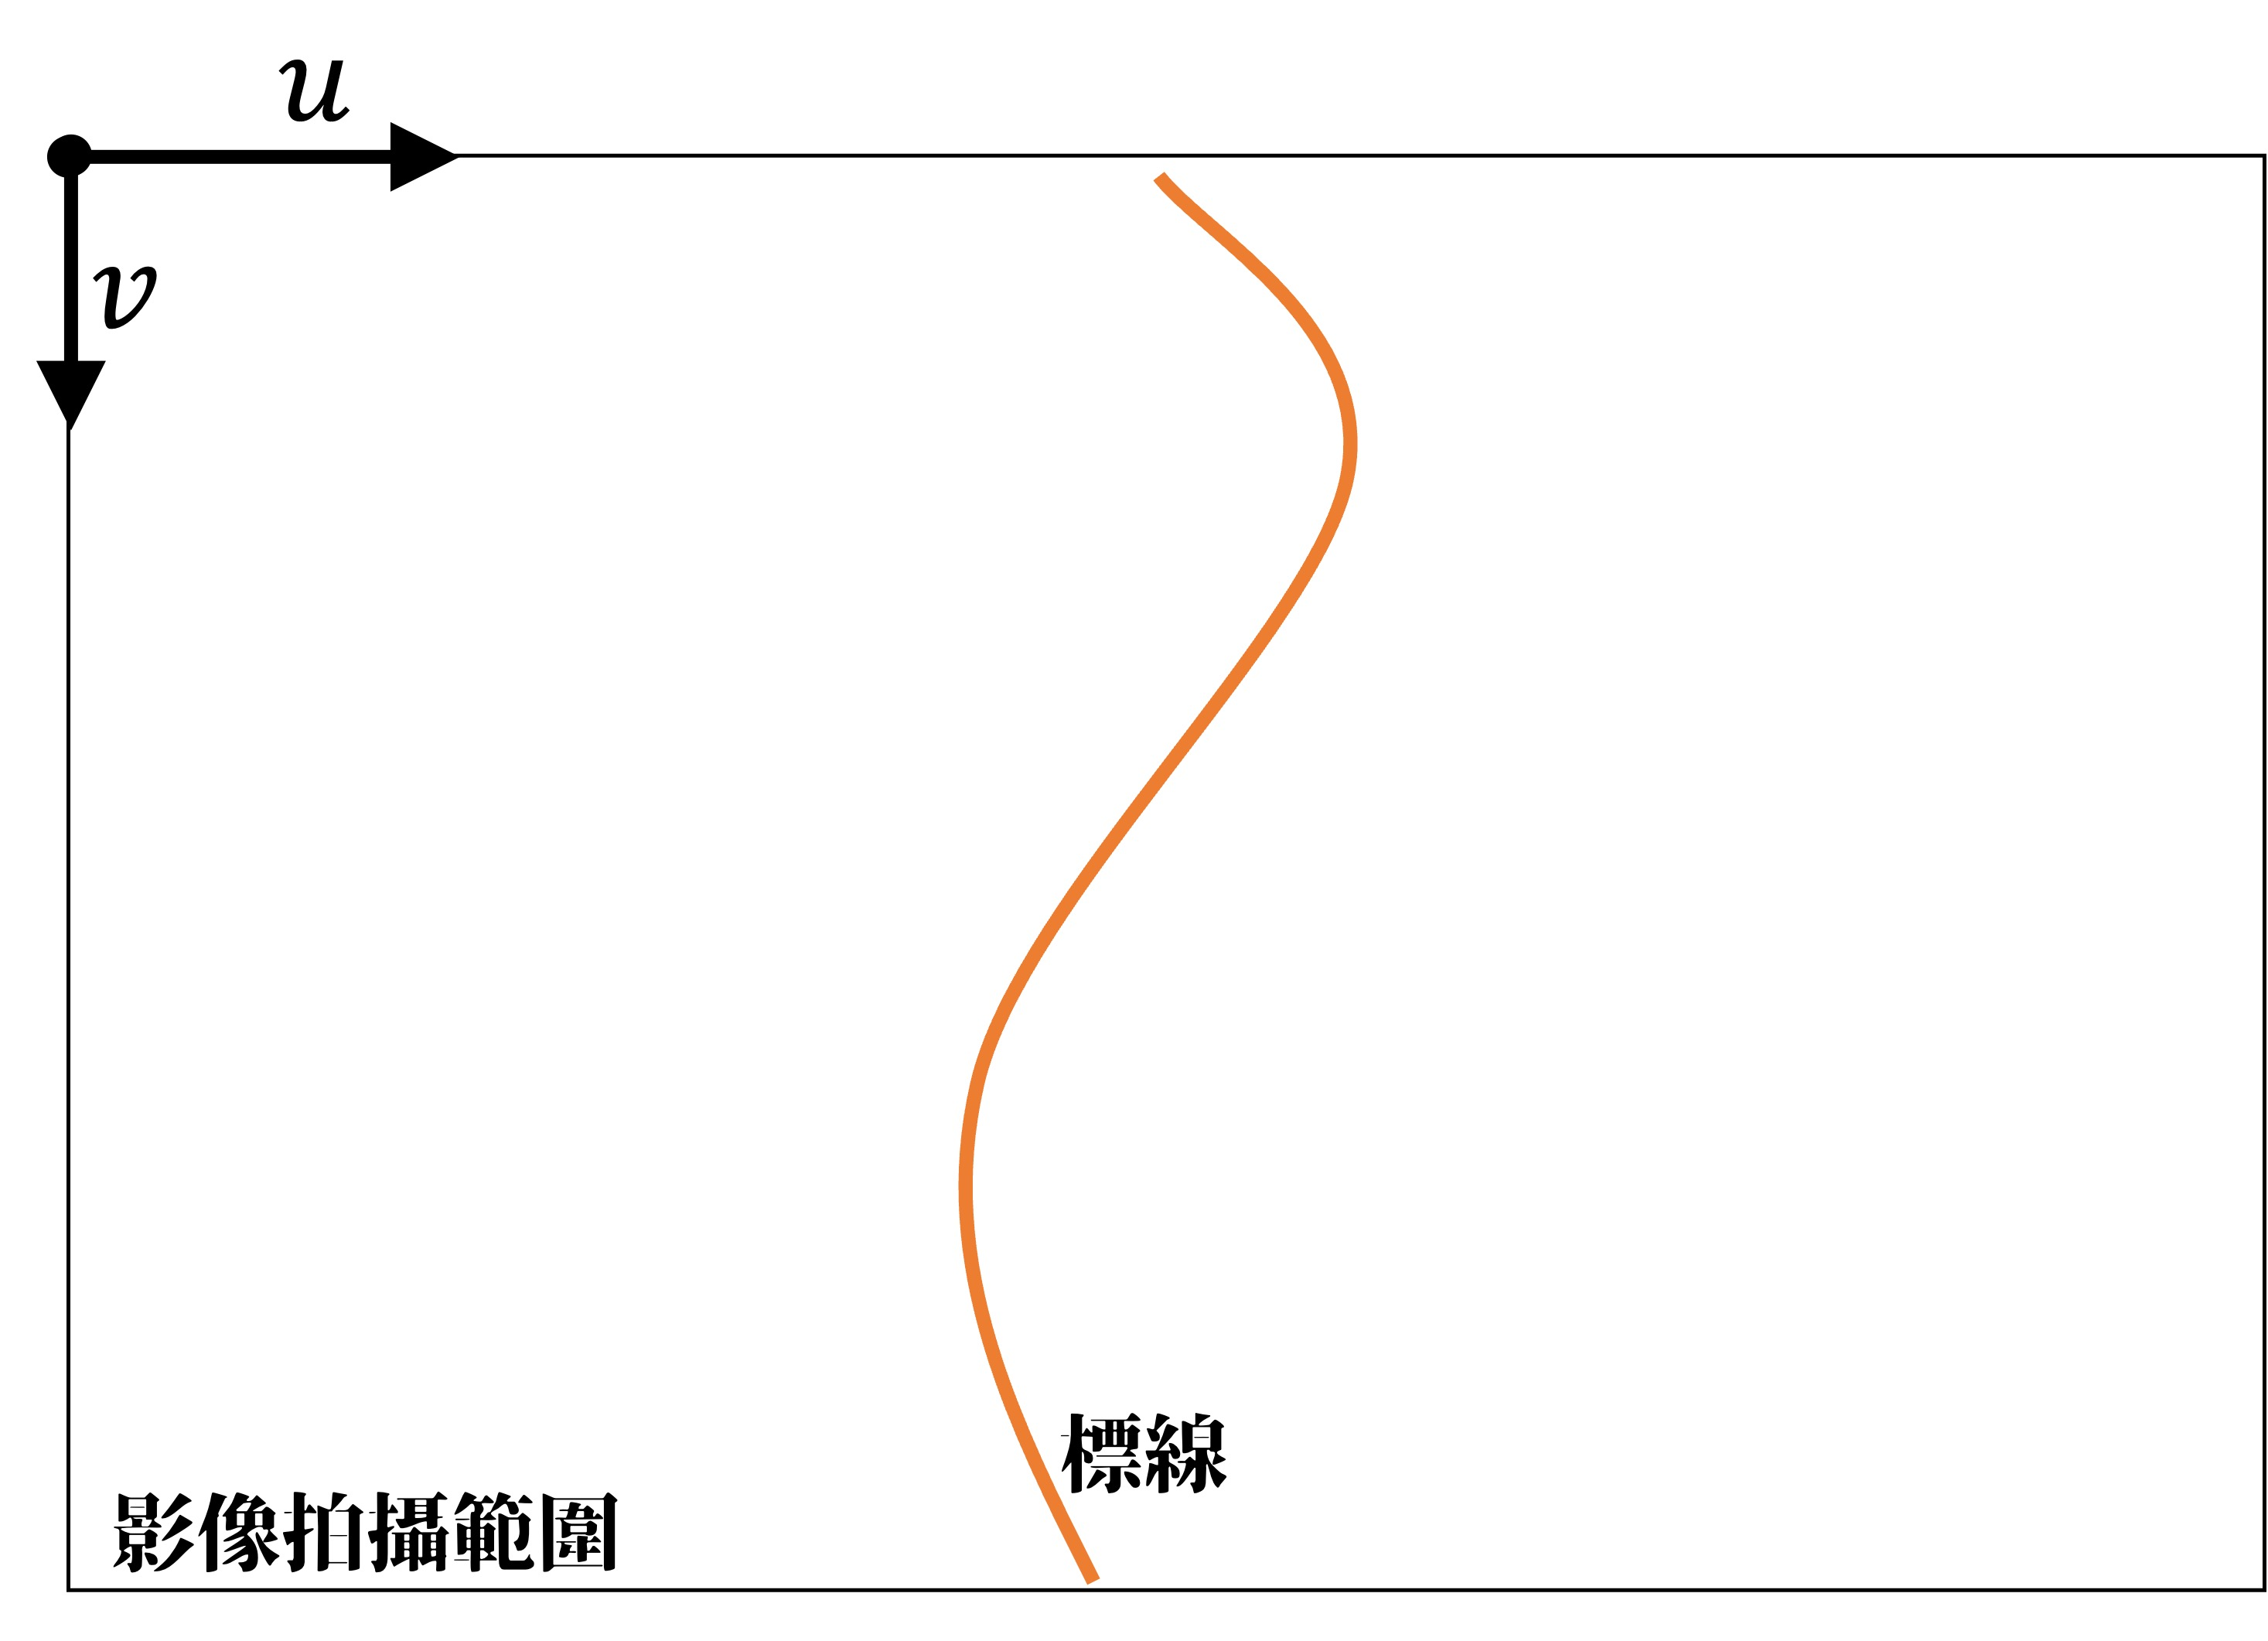
\includegraphics[width=0.7\textwidth]{15.jpg}     %圖片檔案名稱
    \caption{相機拍攝之原始影像}    %圖片檔案名稱
    \label{fig:15}    %為圖片添加標籤
    %如\ref{fig:example1}所示
\end{figure}
\begin{figure}[H]
    \centering
    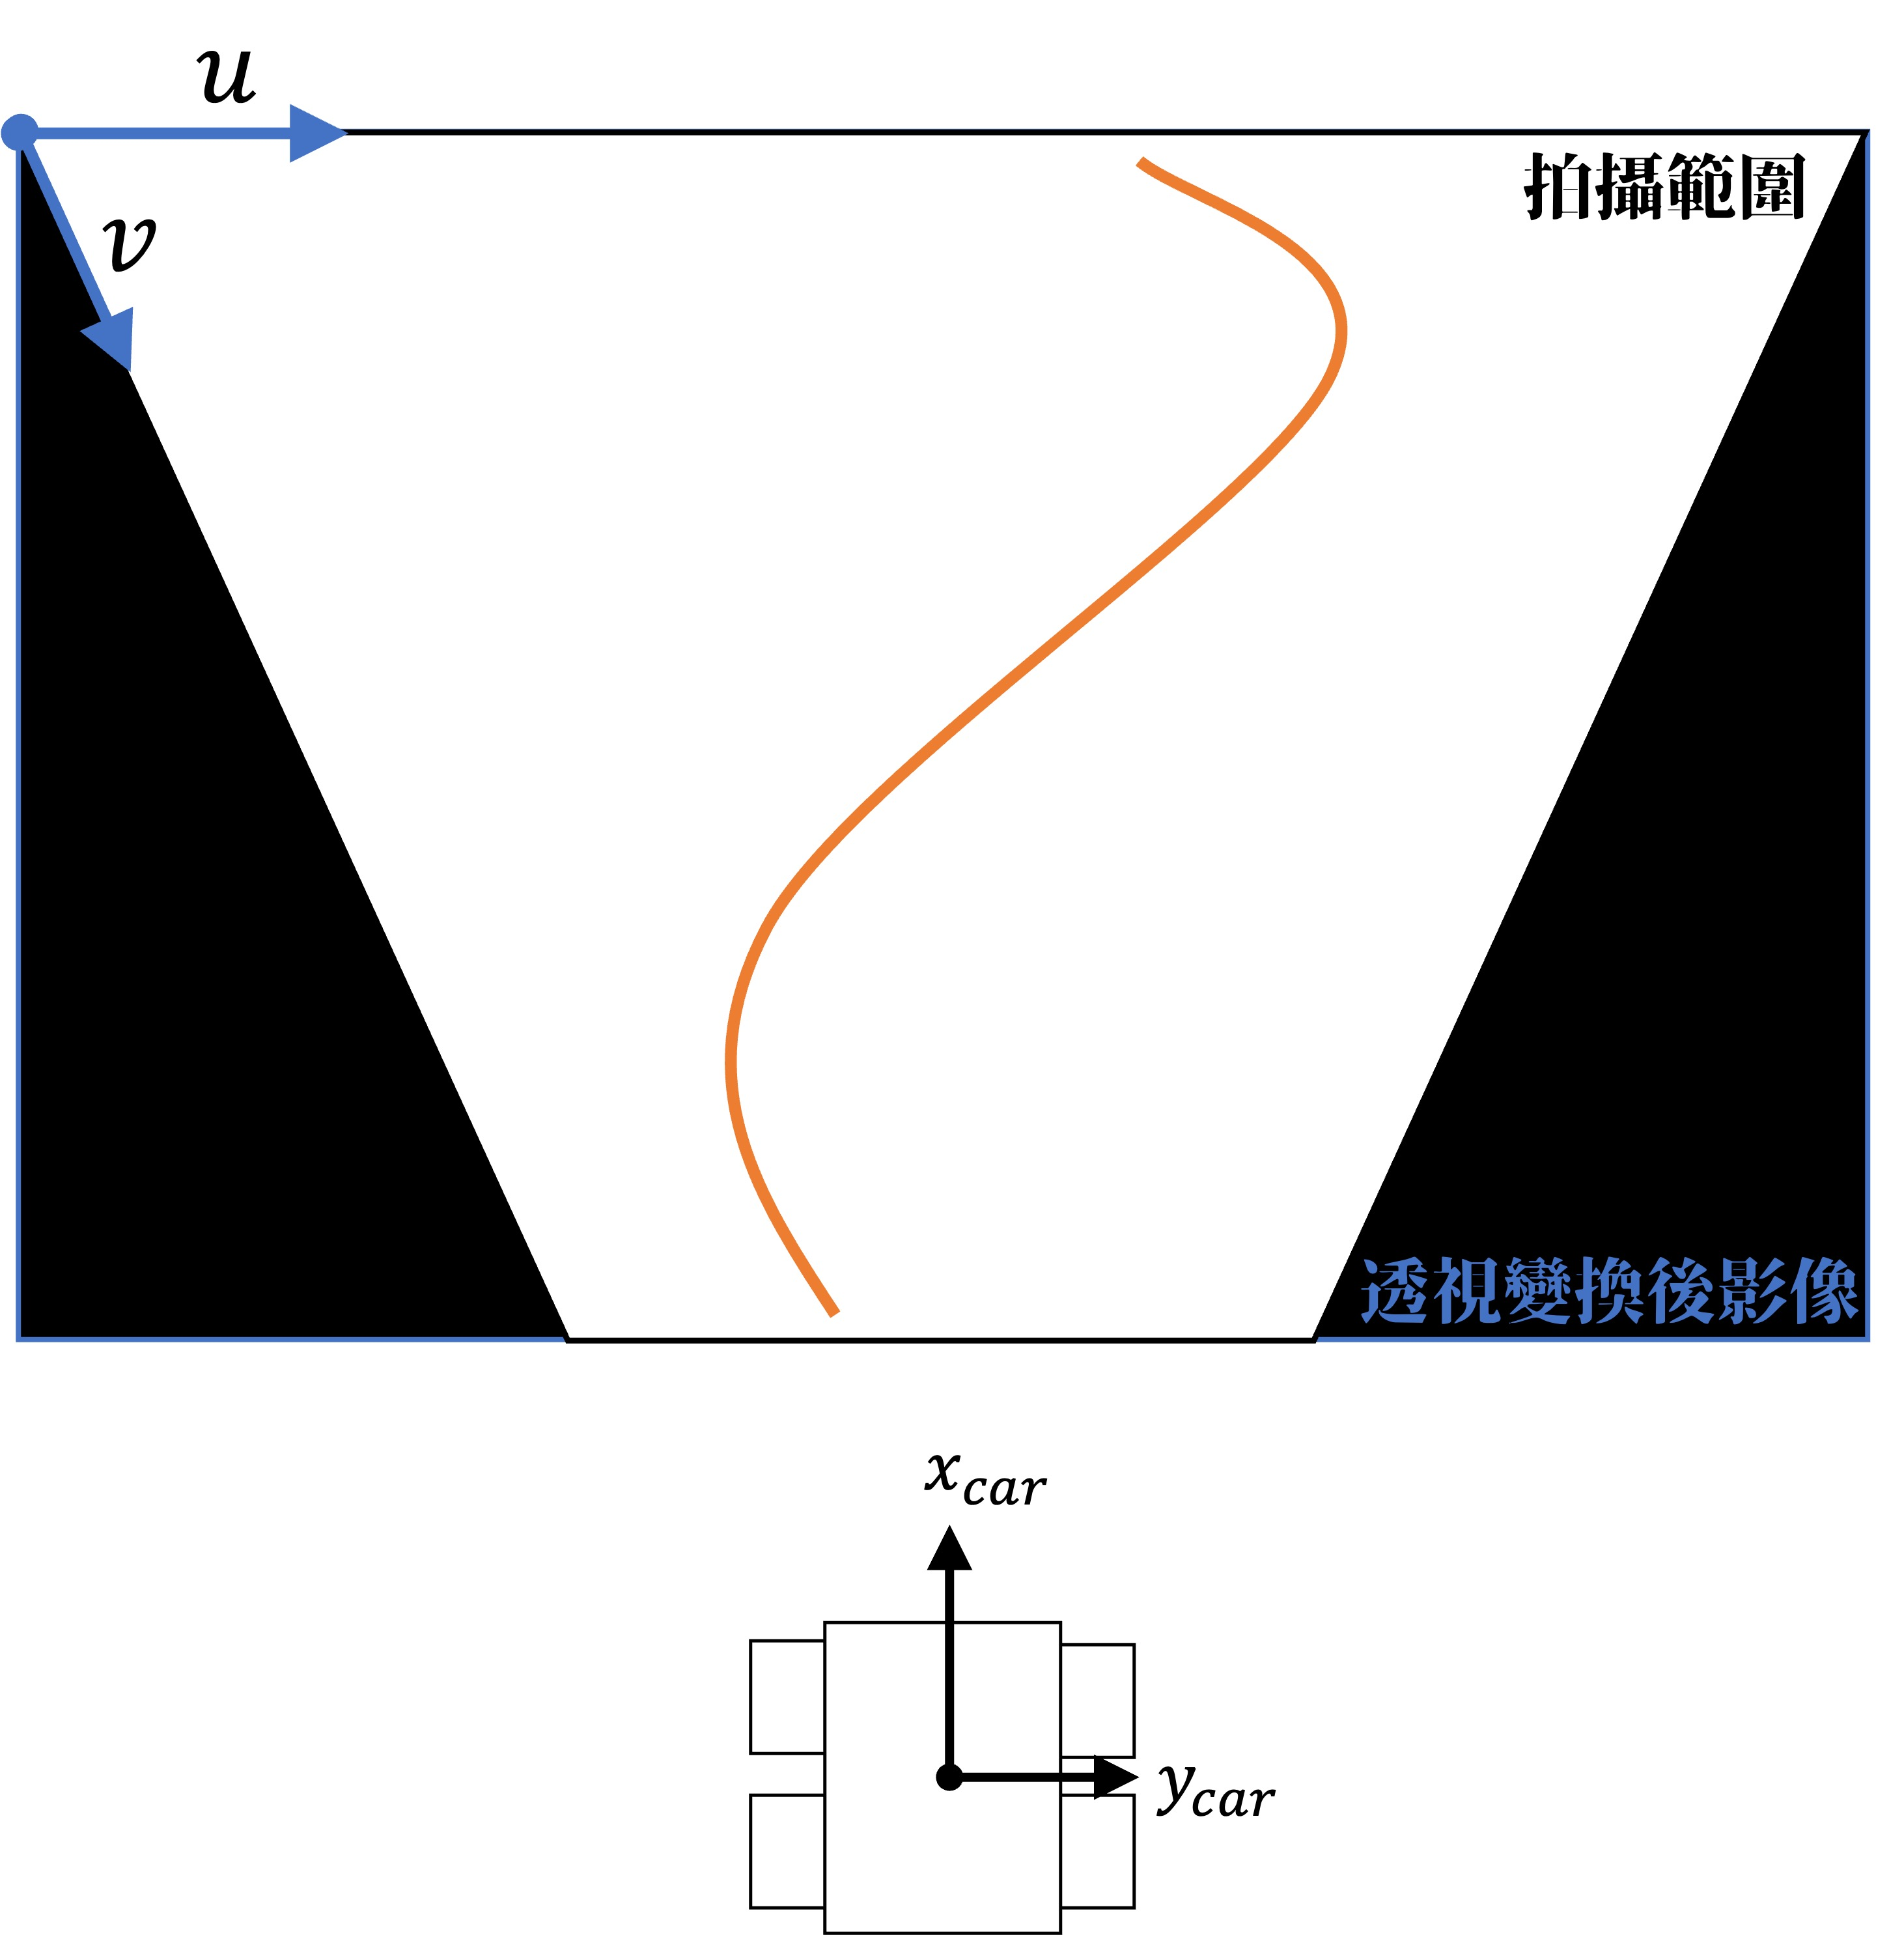
\includegraphics[width=0.7\textwidth]{14.jpg}     %圖片檔案名稱
    \caption{車輛座標系與像素坐標系關係之示意圖}    %圖片檔案名稱
    \label{fig:14}    %為圖片添加標籤
    %如\ref{fig:example1}所示
\end{figure}
將利用鏡頭往斜下的角度拍攝。採用逆透視變換(Inverse Perspective Mapping，IPM)\cite{lin_2001}\cite{bertozz1998stereo}\cite{mallot1991inverse}技術處理影像，可以將像素座標轉換為地面座標，取得影像中精確的距離。

透視變換的核心在於去除透視效應，以便將影像中的道路線條轉換為平行的直線。這樣的變換有助於車輛識別路徑，使後續演算法能夠更容易地進行路徑規劃與車道偵測。

首先將影像像素座標系$(u,v)$轉換為圖像座標系$(x,y)$。
加入相機的水平視角$HFOV$與相機的垂直視角$VFOV$、相機俯仰角$\theta_{camera}$，將圖像座標轉換為相機座標$(x_{camera},y_{camera},z_{camera})$。
接著將相機座標系轉換為車輛標系$(x_{car},y_{car},z_{car})$，以取得拍攝影像中內容物與車輛之相對位置。流程圖如下：
\begin{figure}[H]
    \centering
    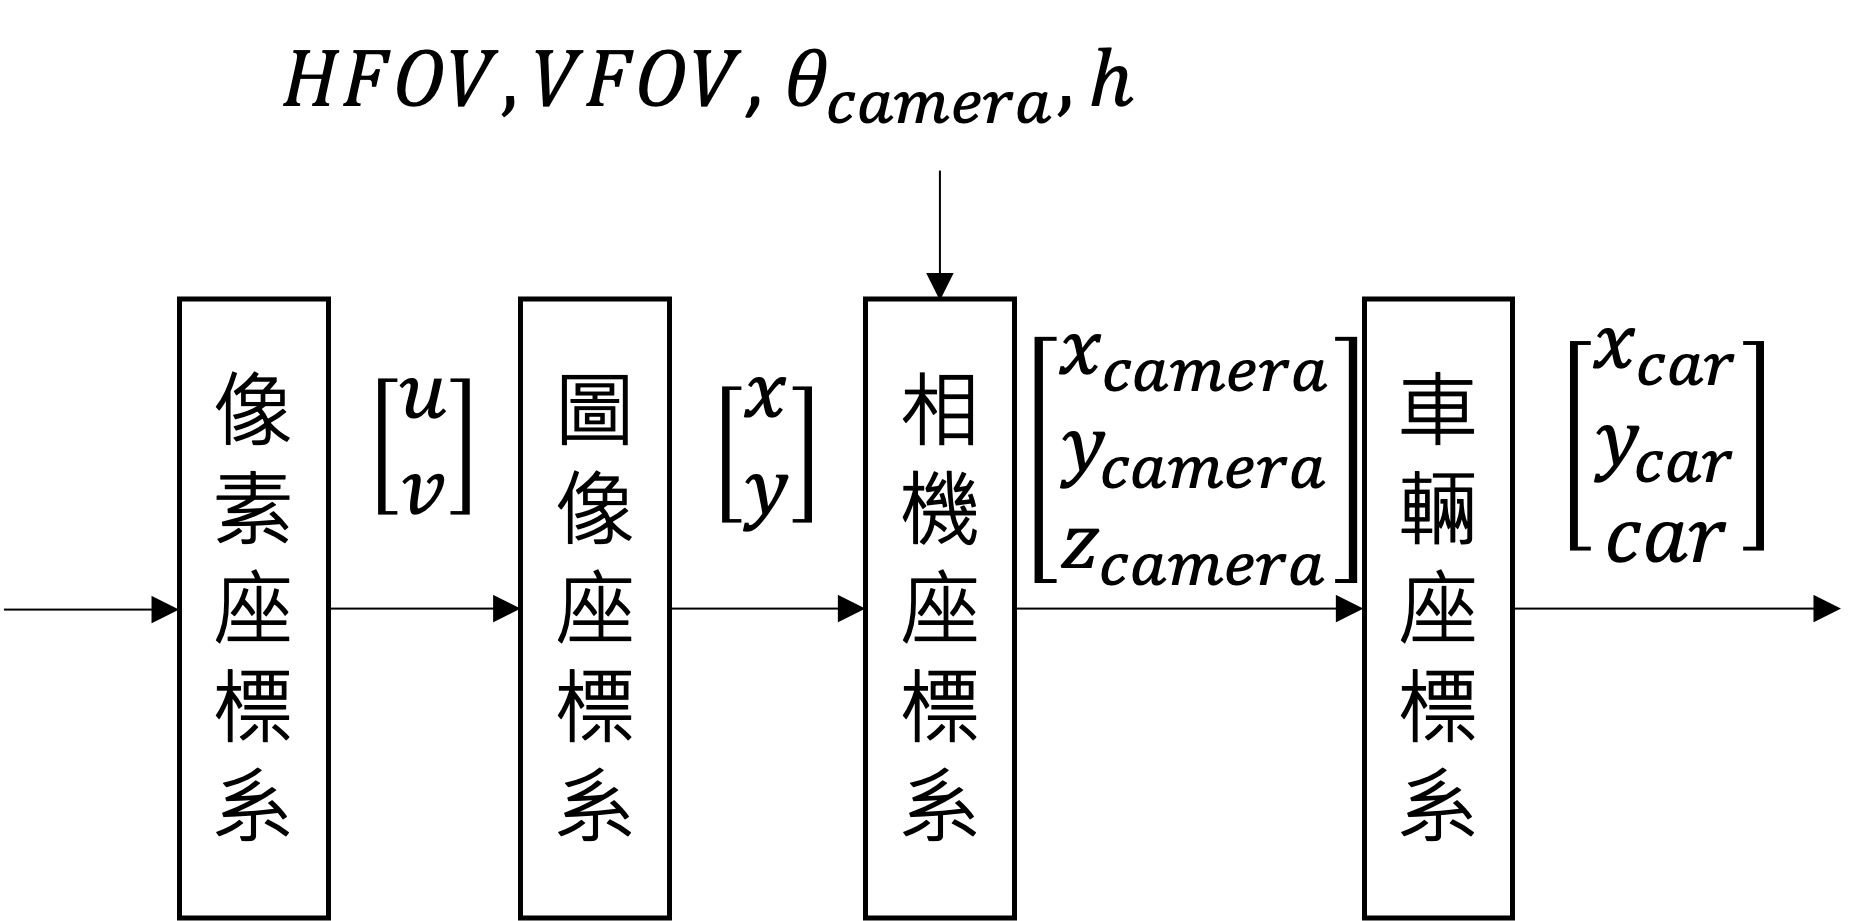
\includegraphics[width=0.7\textwidth]{12.jpg}     %圖片檔案名稱
    \caption{透視變換流程圖}    %圖片檔案名稱
    \label{fig:12}    %為圖片添加標籤
    %如\ref{fig:example1}所示
\end{figure}
將像素座標轉換為無人機相對於地平面的世界座標時，過程涉及相機的內參矩陣$K$、旋轉矩陣$R$以及相機高度$h$。要算相機的內參矩陣首先需得出影像的水平焦距$f_{x}$、影像的垂直焦距$f_{y}$和影像的中心座標$(c_x,c_y)$。

影像的水平焦距$f_{x}$公式如式(\ref{eq:fx})，W為影像的寬度，HFOV為相機的水平視角。
影像的垂直焦距$f_{y}$公式如式(\ref{eq:fy})，H為影像的寬度，VFOV為相機的垂直視角。
\begin{align}
    f_{x}=\frac{W}{2\cdot\tan\left(\frac{HFOV}{2}\right)}
    \label{eq:fx}
    \\
    f_{y}=\frac{H}{2\cdot\tan\left(\frac{VFOV}{2}\right)}
    \label{eq:fy}
\end{align}

影像的中心座標$(c_x,c_y)$公式如式(\ref{eq:cx})、式(\ref{eq:cy})：
\begin{align}
    c_{x}=\frac{W}{2}
    \label{eq:cx}
    \\
    c_{y}=\frac{H}{2}
    \label{eq:cy}
\end{align}

式(\ref{eq:k})為相機內參矩陣K。
\begin{align}
    K &=
    \begin{bmatrix}
        f_{x}       & 0             & c_{x}     \\
        0           & f_{y}         & c_{y}     \\
        0           & 0             & 1
    \end{bmatrix} 
    \label{eq:k}
\end{align}

旋轉矩陣R用來表示相機相對於世界座標系的旋轉。
此處忽略車輛進行中的晃動。旋轉矩陣R如下：
\begin{align}
    R=&
    \begin{bmatrix}
        1   & 0  & 0 \\
        0   & \cos(\theta_{camera})   & -\sin(\theta_{camera}) \\
        0   & \sin(\theta_{camera})   & \cos(\theta_{camera}) \\
    \end{bmatrix} 
    \label{eq:R2}
\end{align}

將像素座標系$(x,y)$轉換為圖像座標系的公式如式(\ref{eq:xy1})：
\begin{align}
    \begin{bmatrix}
        x       \\
        y    \\
        1        
    \end{bmatrix} 
     &=K^{-1}\cdot
     \begin{bmatrix}
        u       \\
        v       \\
        1        
    \end{bmatrix} 
    \label{eq:xy1}
\end{align}

將圖像座標系轉換為相機座標系的公式如式(\ref{eq:xcyczc})：
\begin{align}
    \begin{bmatrix}
        x_{camera}   \\
        y_{camera}   \\
        z_{camera}        
    \end{bmatrix} 
     &=R\cdot
     \begin{bmatrix}
        x       \\
        y       \\
        1        
    \end{bmatrix} 
    \label{eq:xcyczc}
\end{align}
將相機座標系轉換為車輛座標系$(x_{car},y_{wcar},z_{wcar})$的公式見式式(\ref{eq:xw})、式式(\ref{eq:yw})，此公式即可獲已車輛為原點的座標系統，取得每影像中每一像素與車輛的絕對距離。
\begin{align}
    x_{w}=\frac{x_{c}}{z_{c}}
    \label{eq:xw}\\
    y_{w}=\frac{y_{c}}{z_{c}}
    \label{eq:yw}
\end{align}

灰階處理將彩色影像轉換為灰階影像，這樣能有效減少計算量，同時保留影像的基本結構特徵，便於後續處理。
這樣的轉換方式基於人眼對不同顏色敏感度的權重選擇，使得轉換後的影像仍然保持較高的可辨識度。

高斯模糊用來去除影像中的噪聲，這有助於平滑影像，減少後續處理中的干擾，尤其是在邊緣檢測時。
高斯模糊的公式如下：
\begin{align}
G(x,y) = \frac{1}{2\pi\sigma^2} e^{-\frac{x^2 + y^2}{2\sigma^2}}
\end{align}
其中，$\sigma$ 為標準差，決定模糊的強度。較大的 $\sigma$ 值會導致更強的平滑效果，但可能會模糊掉重要的邊緣資訊。

二值化將影像轉換為二值圖像，即只保留黑白兩種顏色，這有助於強調出車道線等重要特徵，便於後續的分析與處理。
固定閾值法：設定一個固定的閾值 $T$，當像素強度高於 $T$ 時設為白色，否則設為黑色。固定閾值法的公式如下。

\begin{align}
    I_{bin}(x,y) = 
    \begin{cases}
        1, & I(x,y) > T \\
        0, & I(x,y) \leq T
    \end{cases}
\end{align}

最後使用Canny 邊緣偵測來提取影像中的邊緣信息，這有助於識別出車道的邊界或其他障礙物，為自走車的導航提供關鍵信息。
%==============================內文==============================

\subsubsection{偵測}
%==============================內文==============================
\hspace{2em}圖像經過預處理後，接下來的步驟是偵測車道標線，並計算車輛的偏移量與偏移角度。

將首先，從影像中掃描特定的區域，通過檢測這些區域的像素值來獲取相關的幾何特徵。
在偵測車道標線時，並非整張影像都具有相同的重要性，因此可以選擇關鍵區域進行分析。例如，車輛前方的道路中央區域可能包含主要的行駛標線，而影像上方區域則可能包含過多的背景資訊，對偵測無實質幫助。
將使用滑動視窗法，使用固定大小的窗口在影像中移動，對每個區域進行局掃描，以提取潛在的車道標線位置，並將視窗滑動偵測最多白色像素之位置。
\begin{figure}[H]
    \centering
    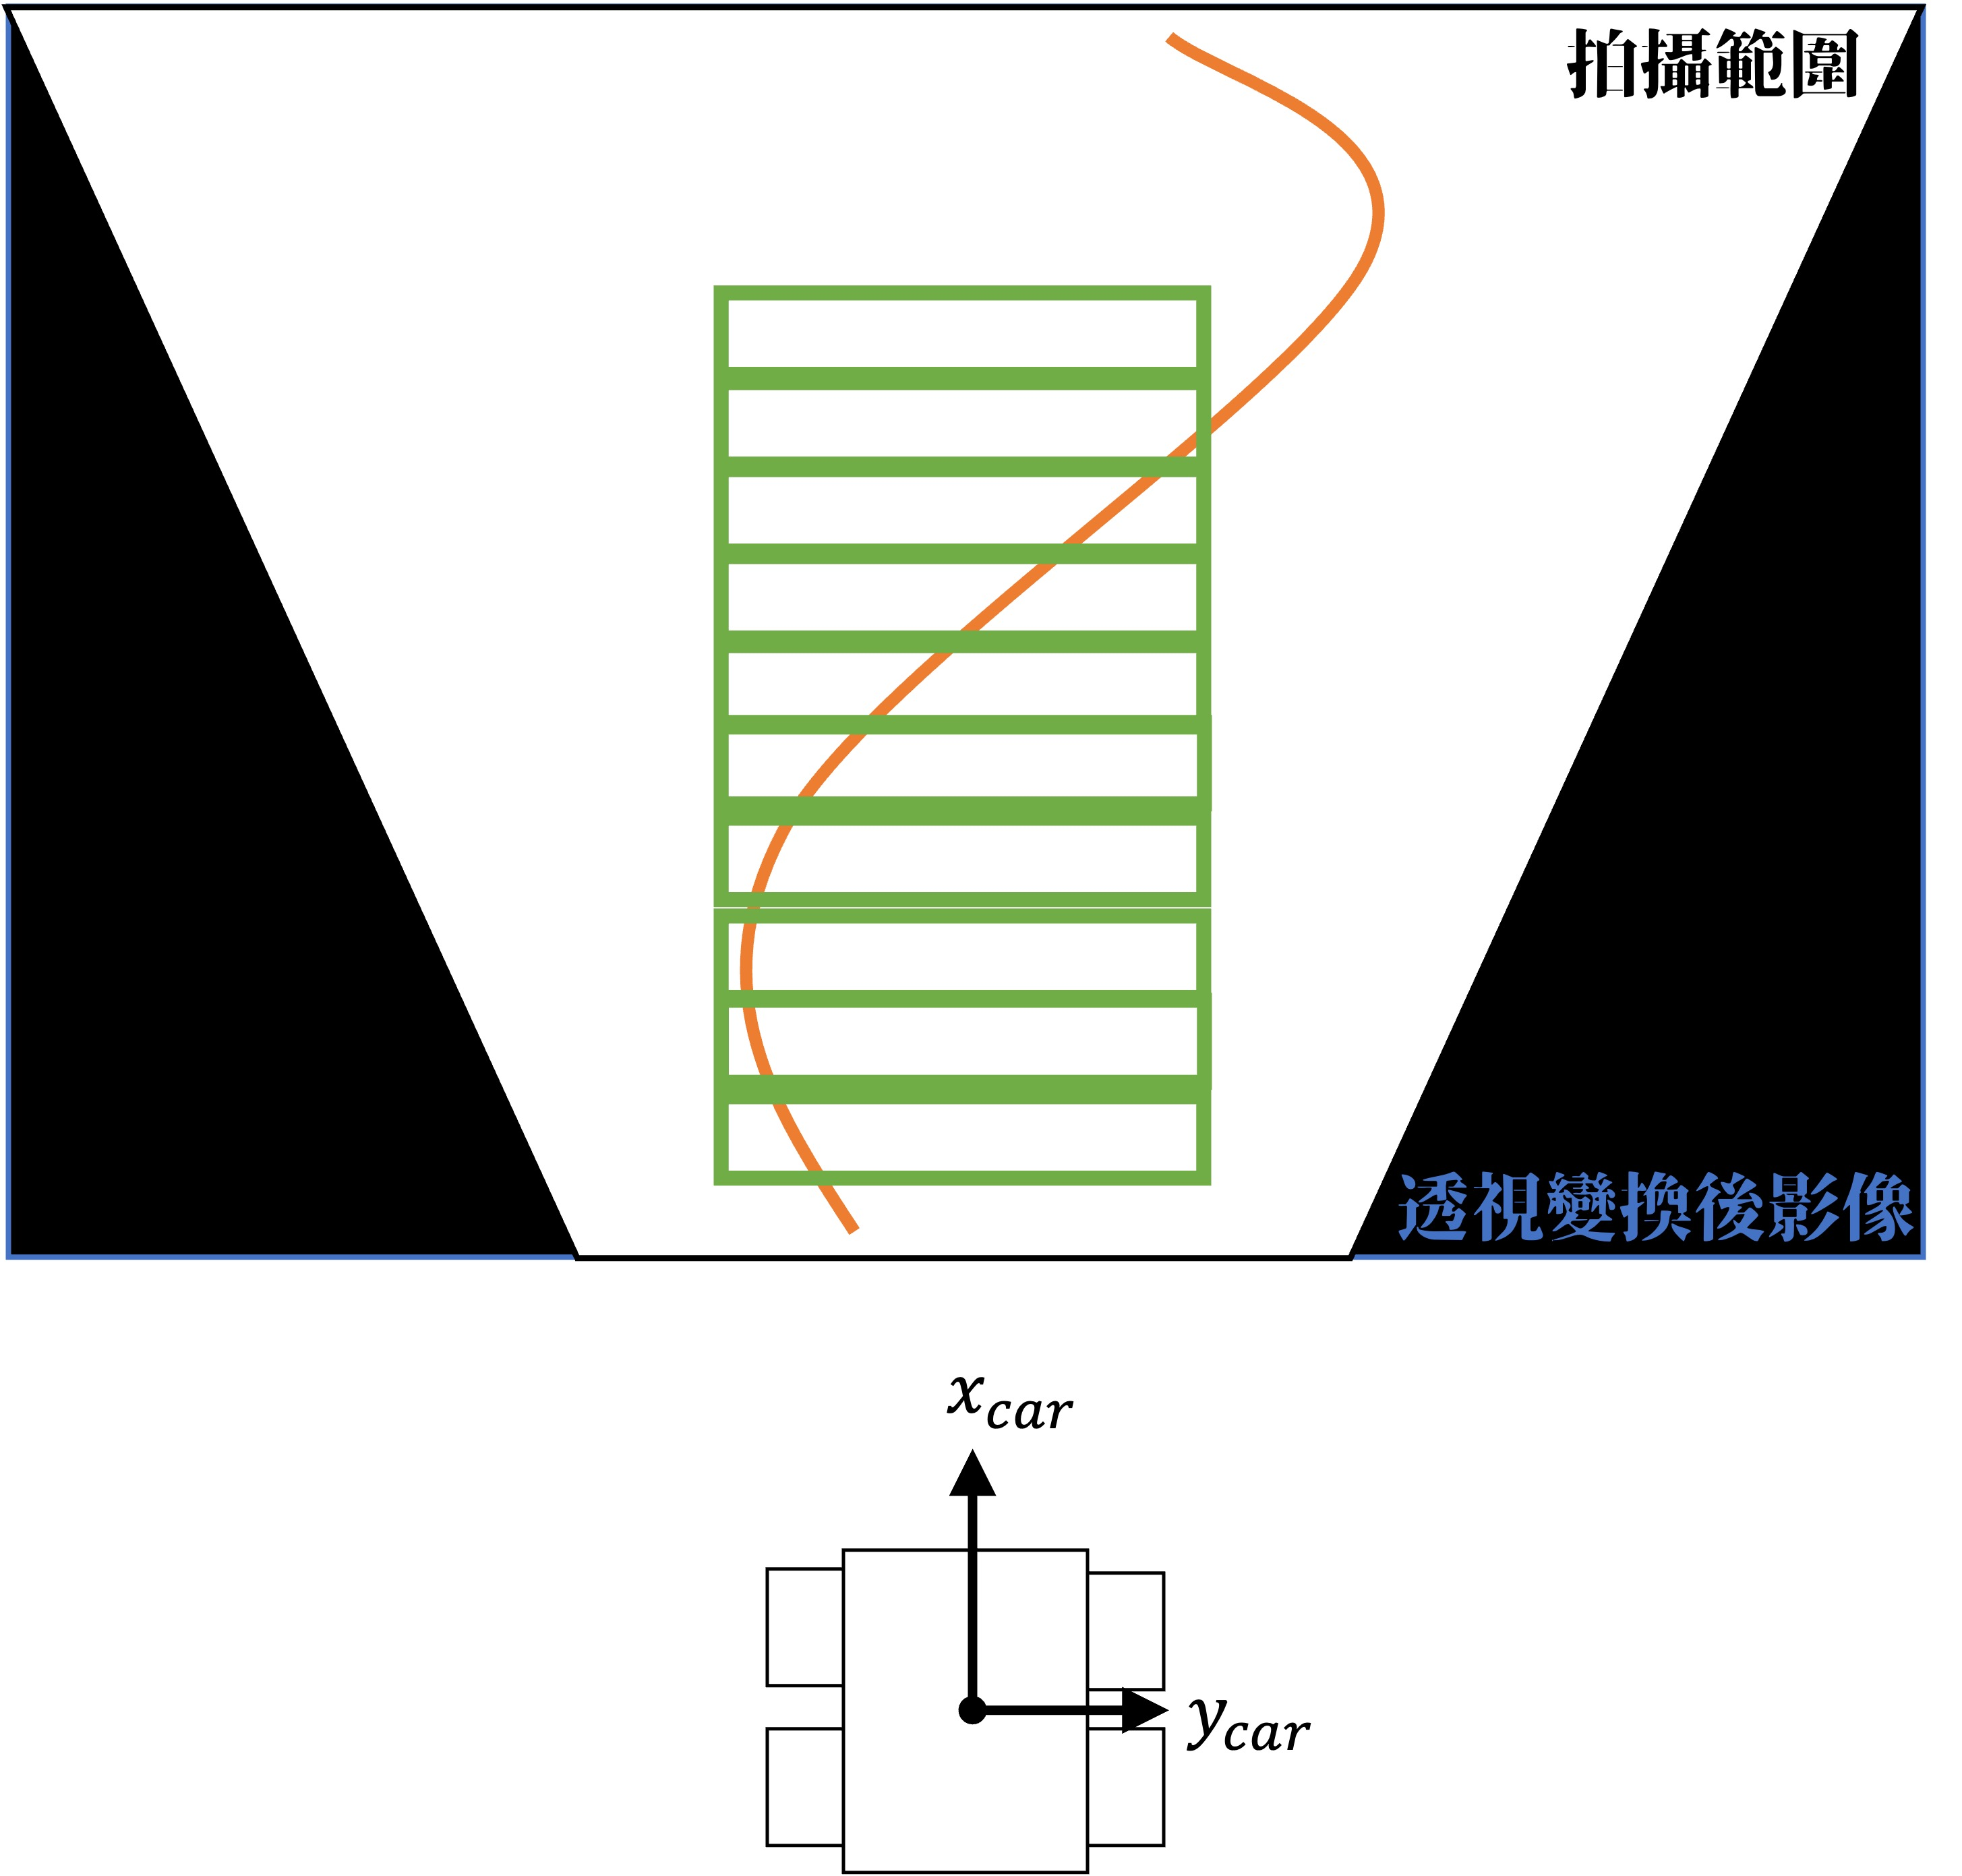
\includegraphics[width=0.7\textwidth]{16.jpg}     %圖片檔案名稱
    \caption{尚未滑動之偵測視窗}    %圖片檔案名稱
    \label{fig:16}    %為圖片添加標籤
    %如\ref{fig:example1}所示
\end{figure}

\begin{figure}[H]
    \centering
    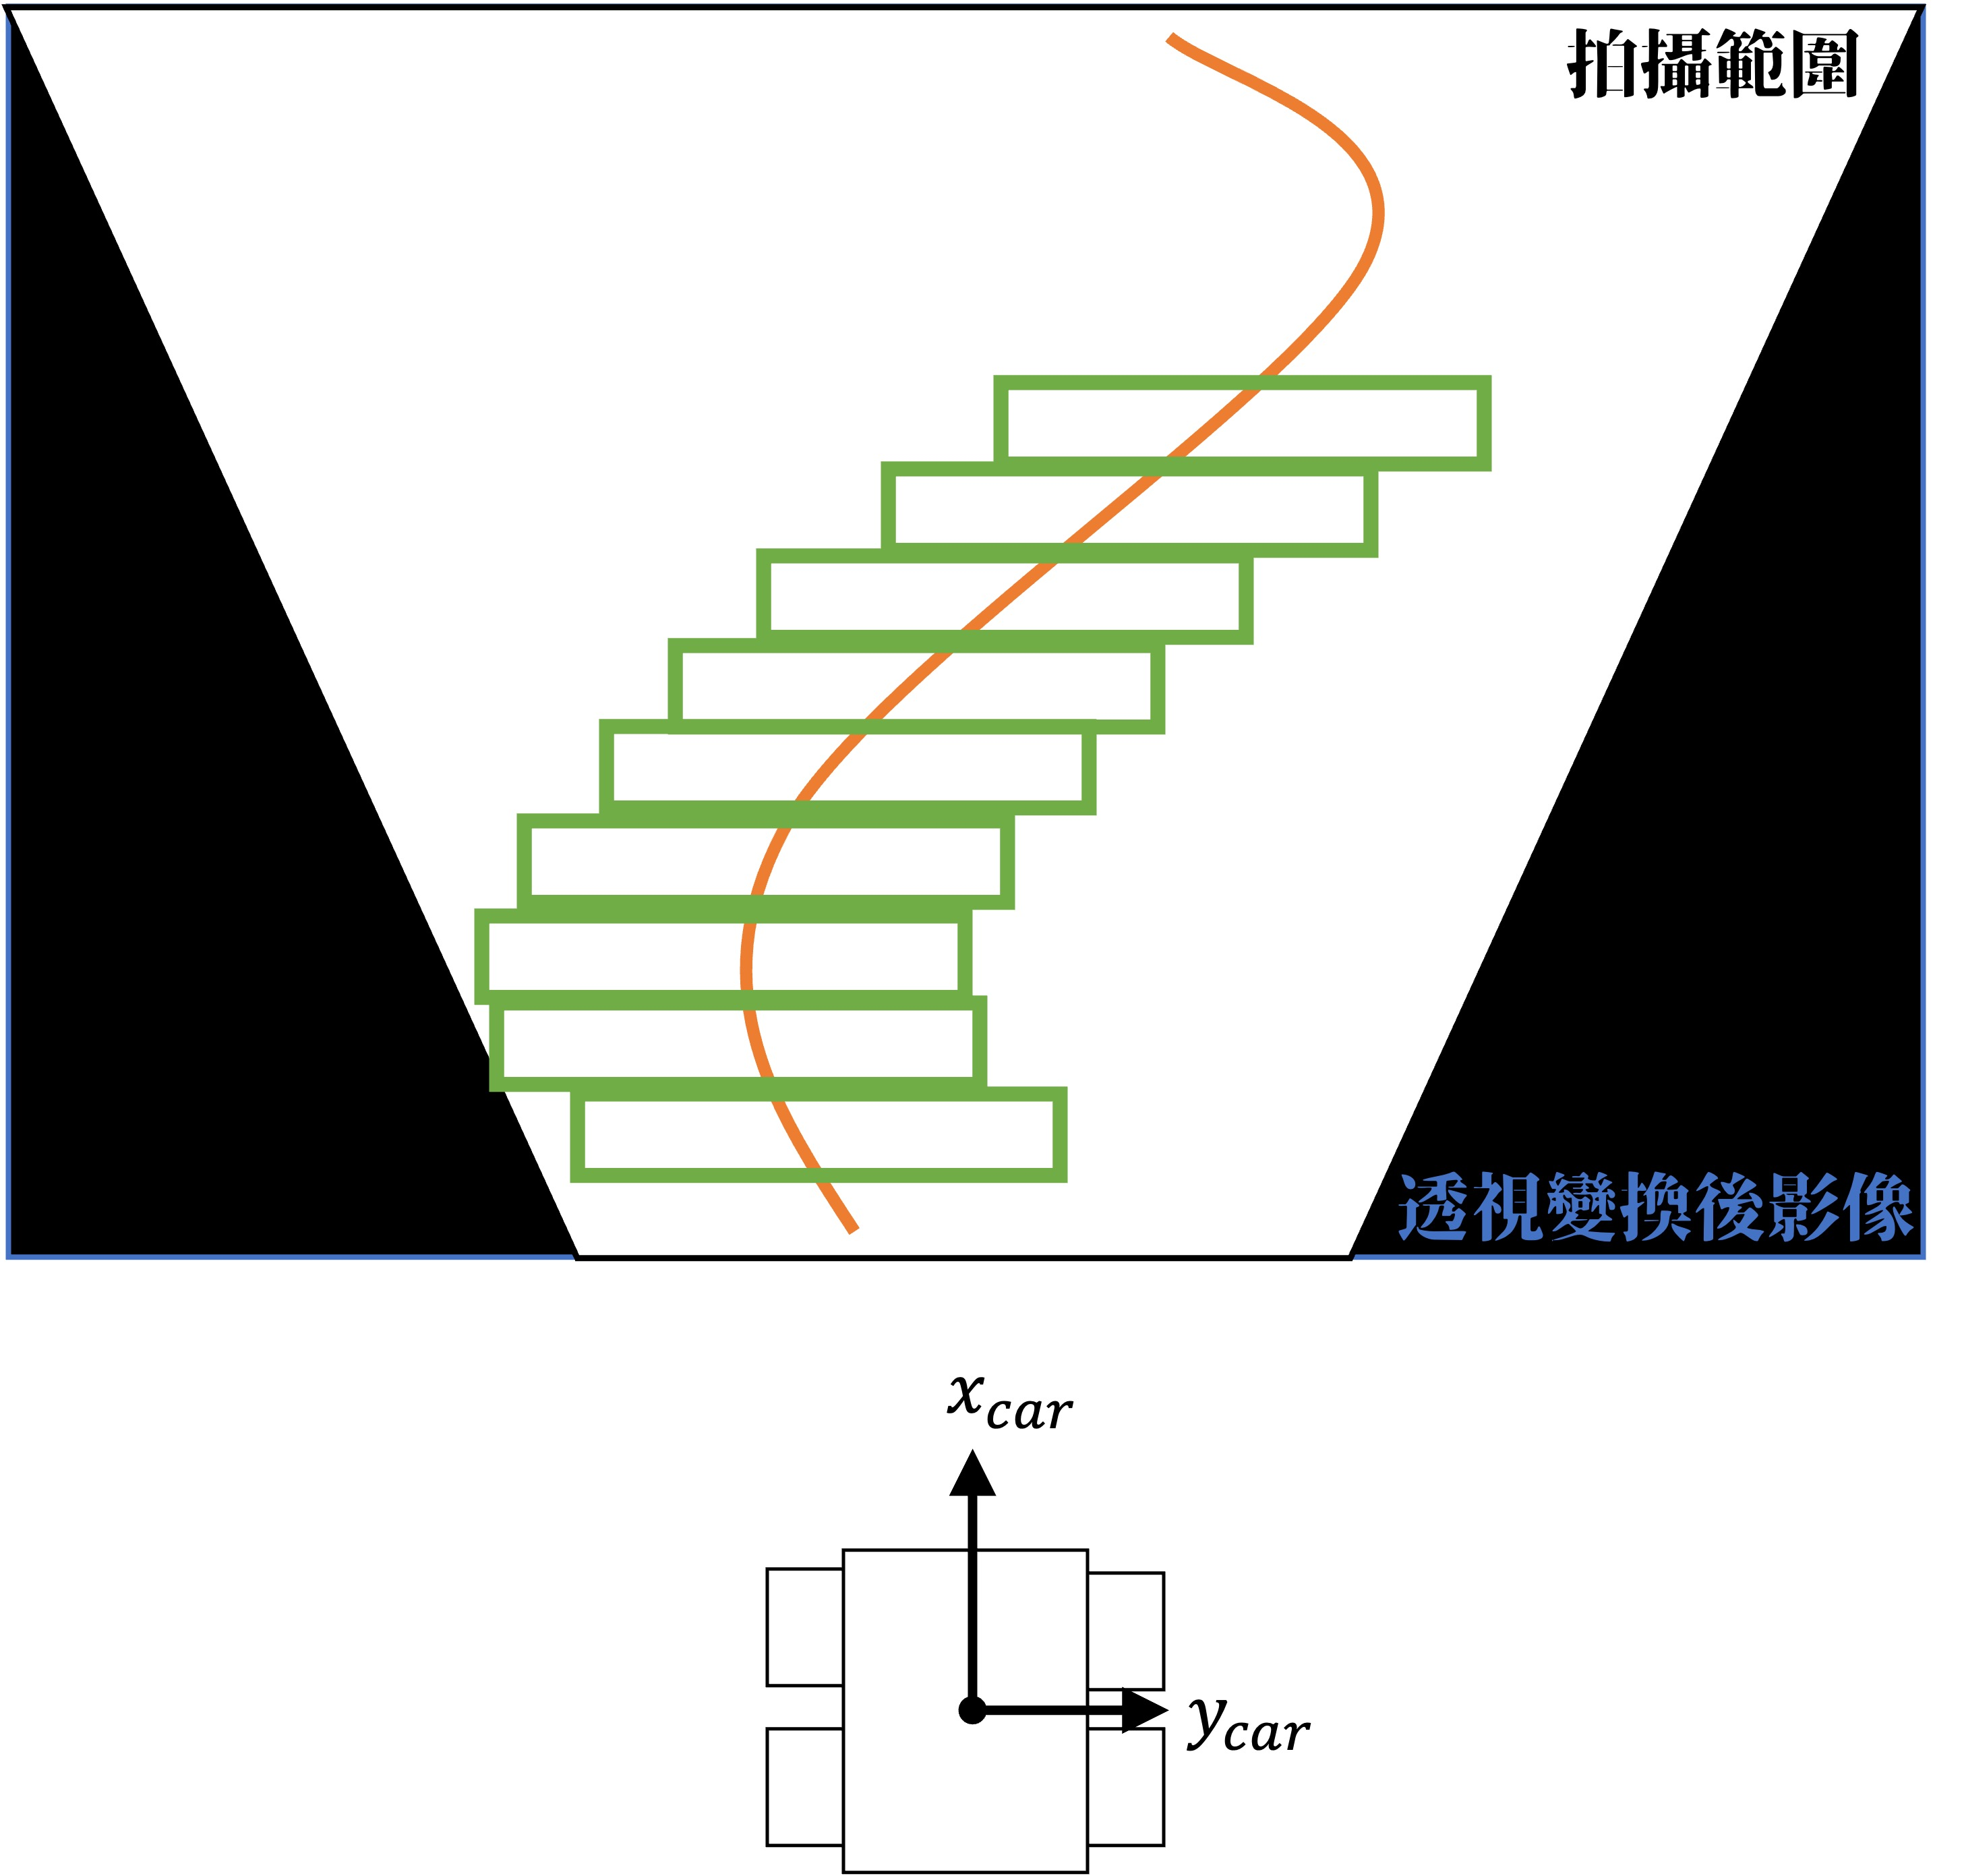
\includegraphics[width=0.7\textwidth]{17.jpg}     %圖片檔案名稱
    \caption{滑動後之偵測視窗}    %圖片檔案名稱
    \label{fig:17}    %為圖片添加標籤
    %如\ref{fig:example1}所示
\end{figure}

據掃描到的像素資料，使用多項式擬合來擬合出車道線或相關物體的曲線，這樣可以準確地描述其形狀。
當獲取到標線像素點後，下一步是利用數學模型來擬合標線的形狀。由於車道標線通常具有一定的連續性與平滑度，可以使用 多項式擬合（Polynomial Fitting） 來描述其形狀。

\hspace{2em}對於普通道路，車道標線通常可以近似為二次曲線： \begin{align} y = ax^2 + bx + c \end{align} 其中，
$a,b,c$ 為待求的係數。使用最小二乘法（Least Squares Method, LSM） 來找到最適合這些數據點的曲線。
\begin{figure}[H]
    \centering
    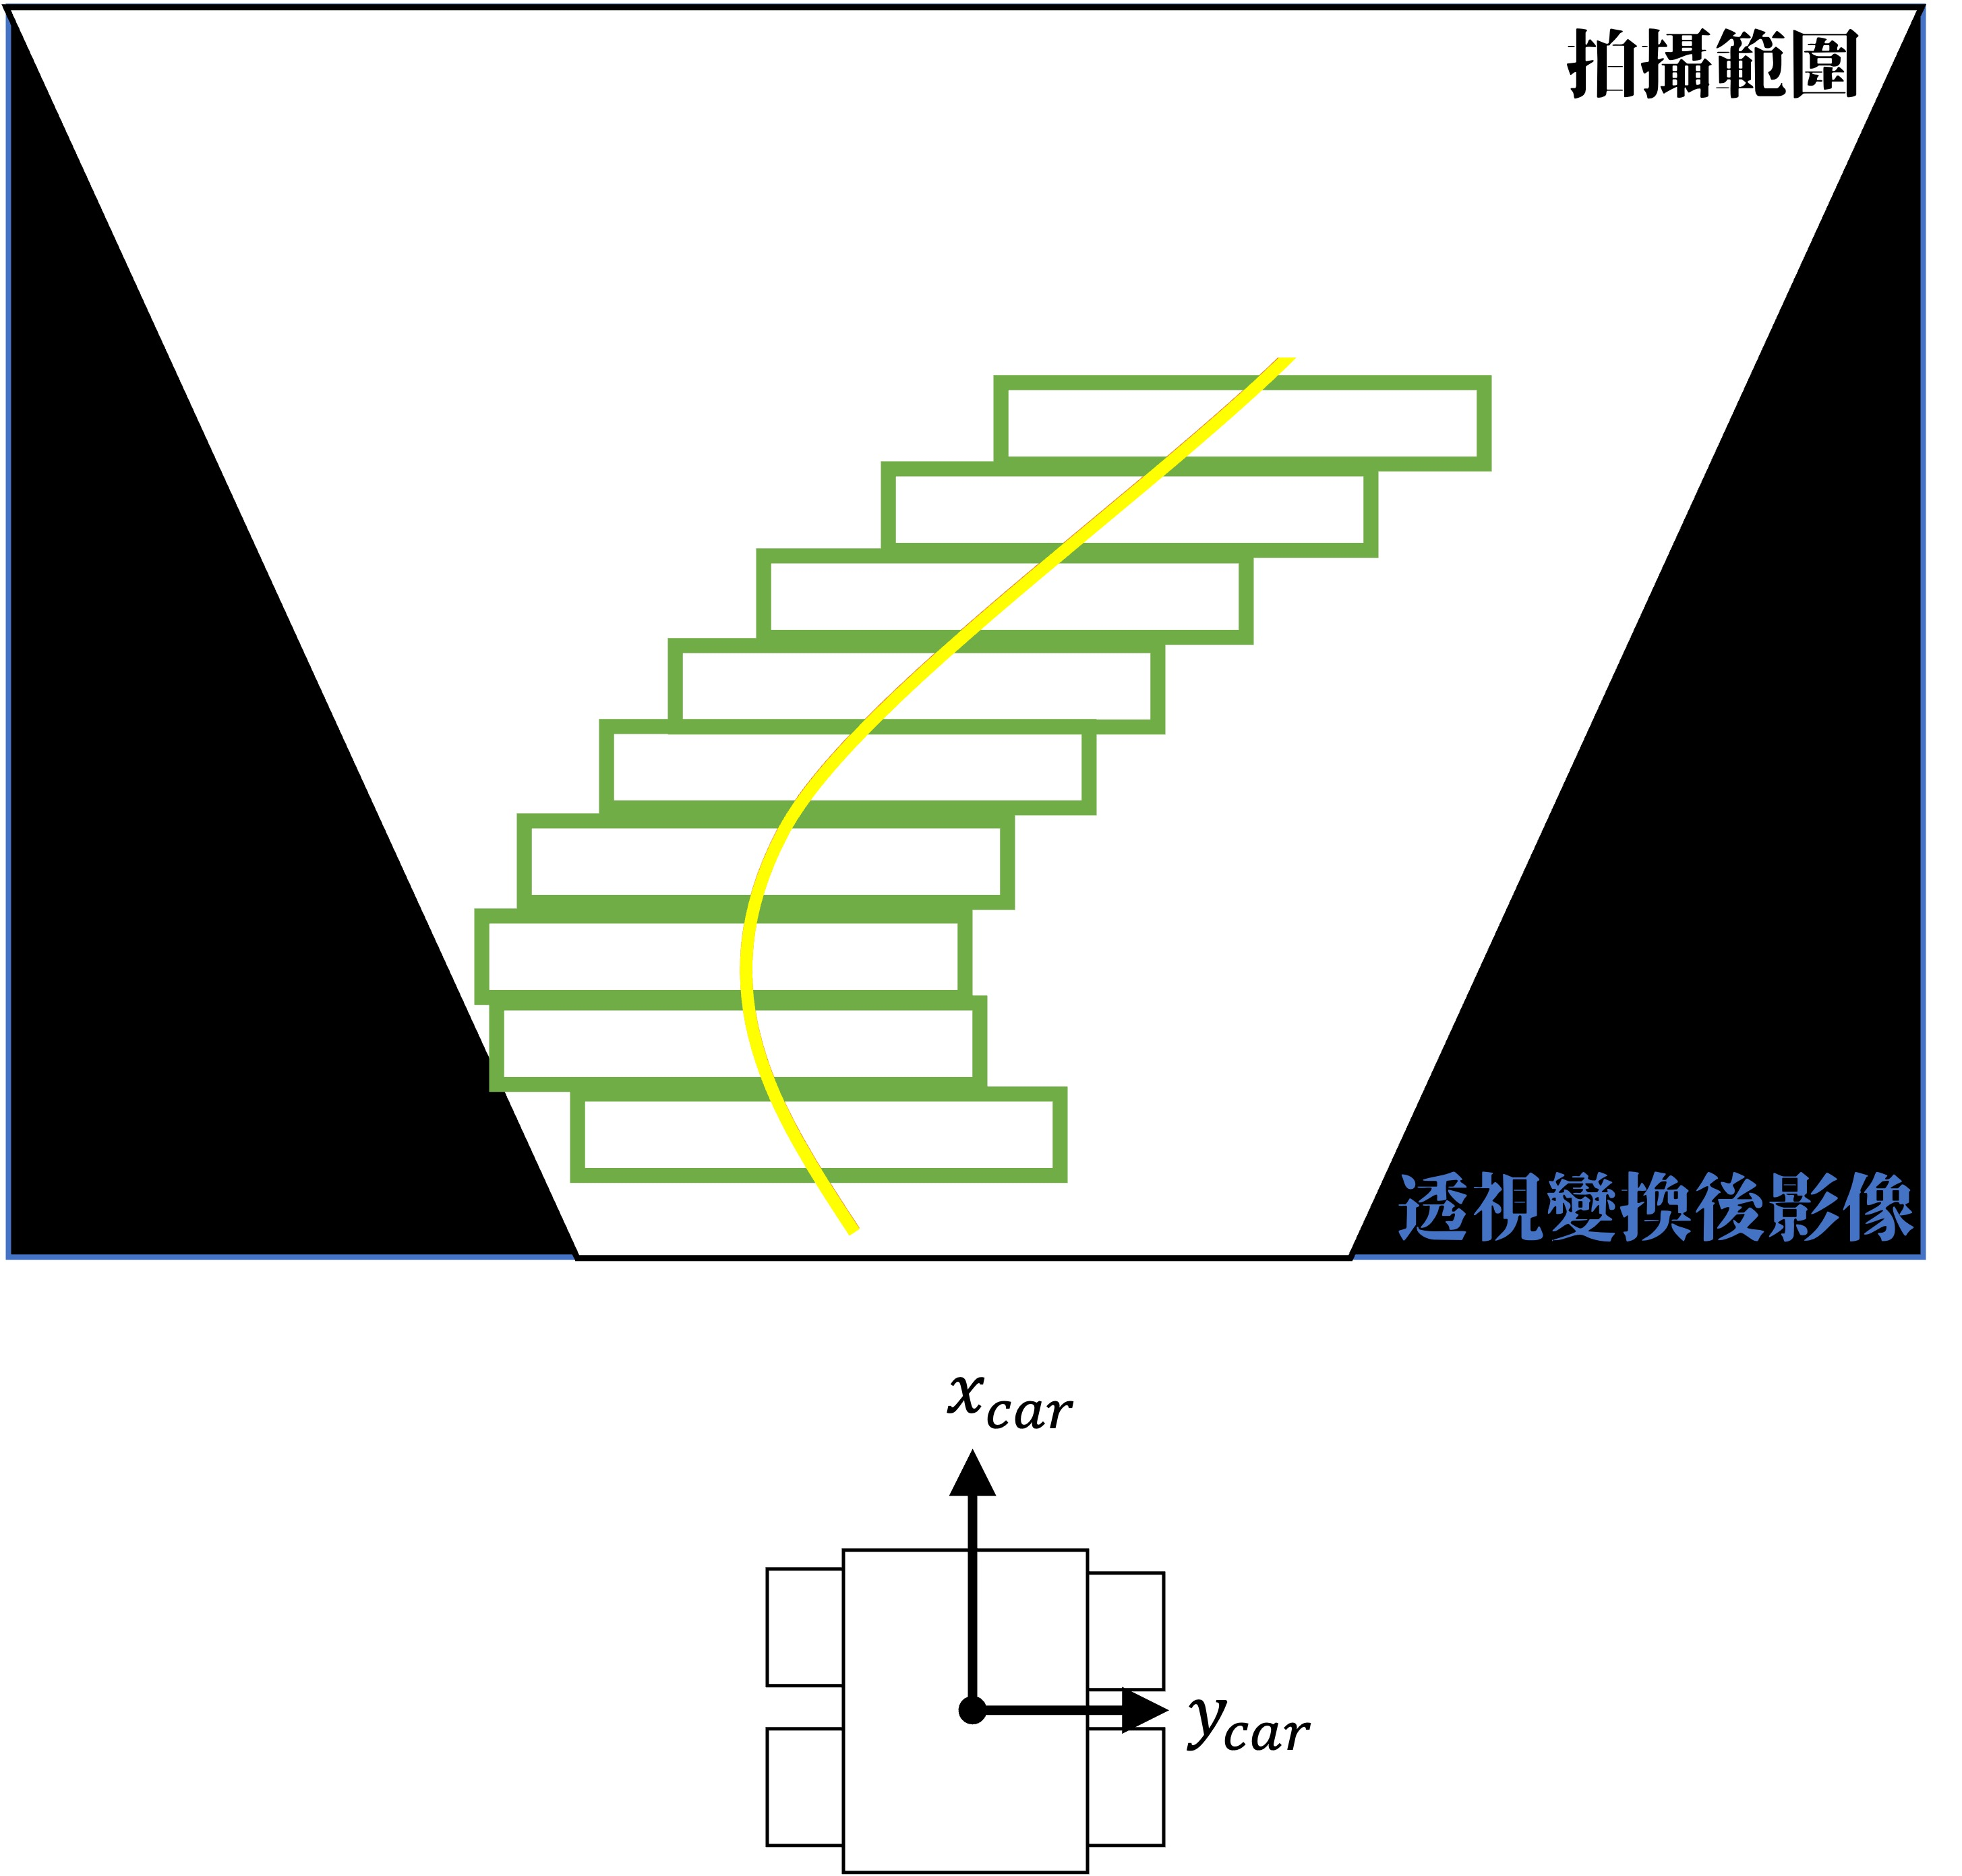
\includegraphics[width=0.7\textwidth]{18.jpg}     %圖片檔案名稱
    \caption{擬合後曲線}    %圖片檔案名稱
    \label{fig:18}    %為圖片添加標籤
    %如\ref{fig:example1}所示
\end{figure}

最後即可根據擬合的曲線與車輛座標系之$x$軸計算車輛的偏移量與偏移角度。

\begin{figure}[H]
    \centering
    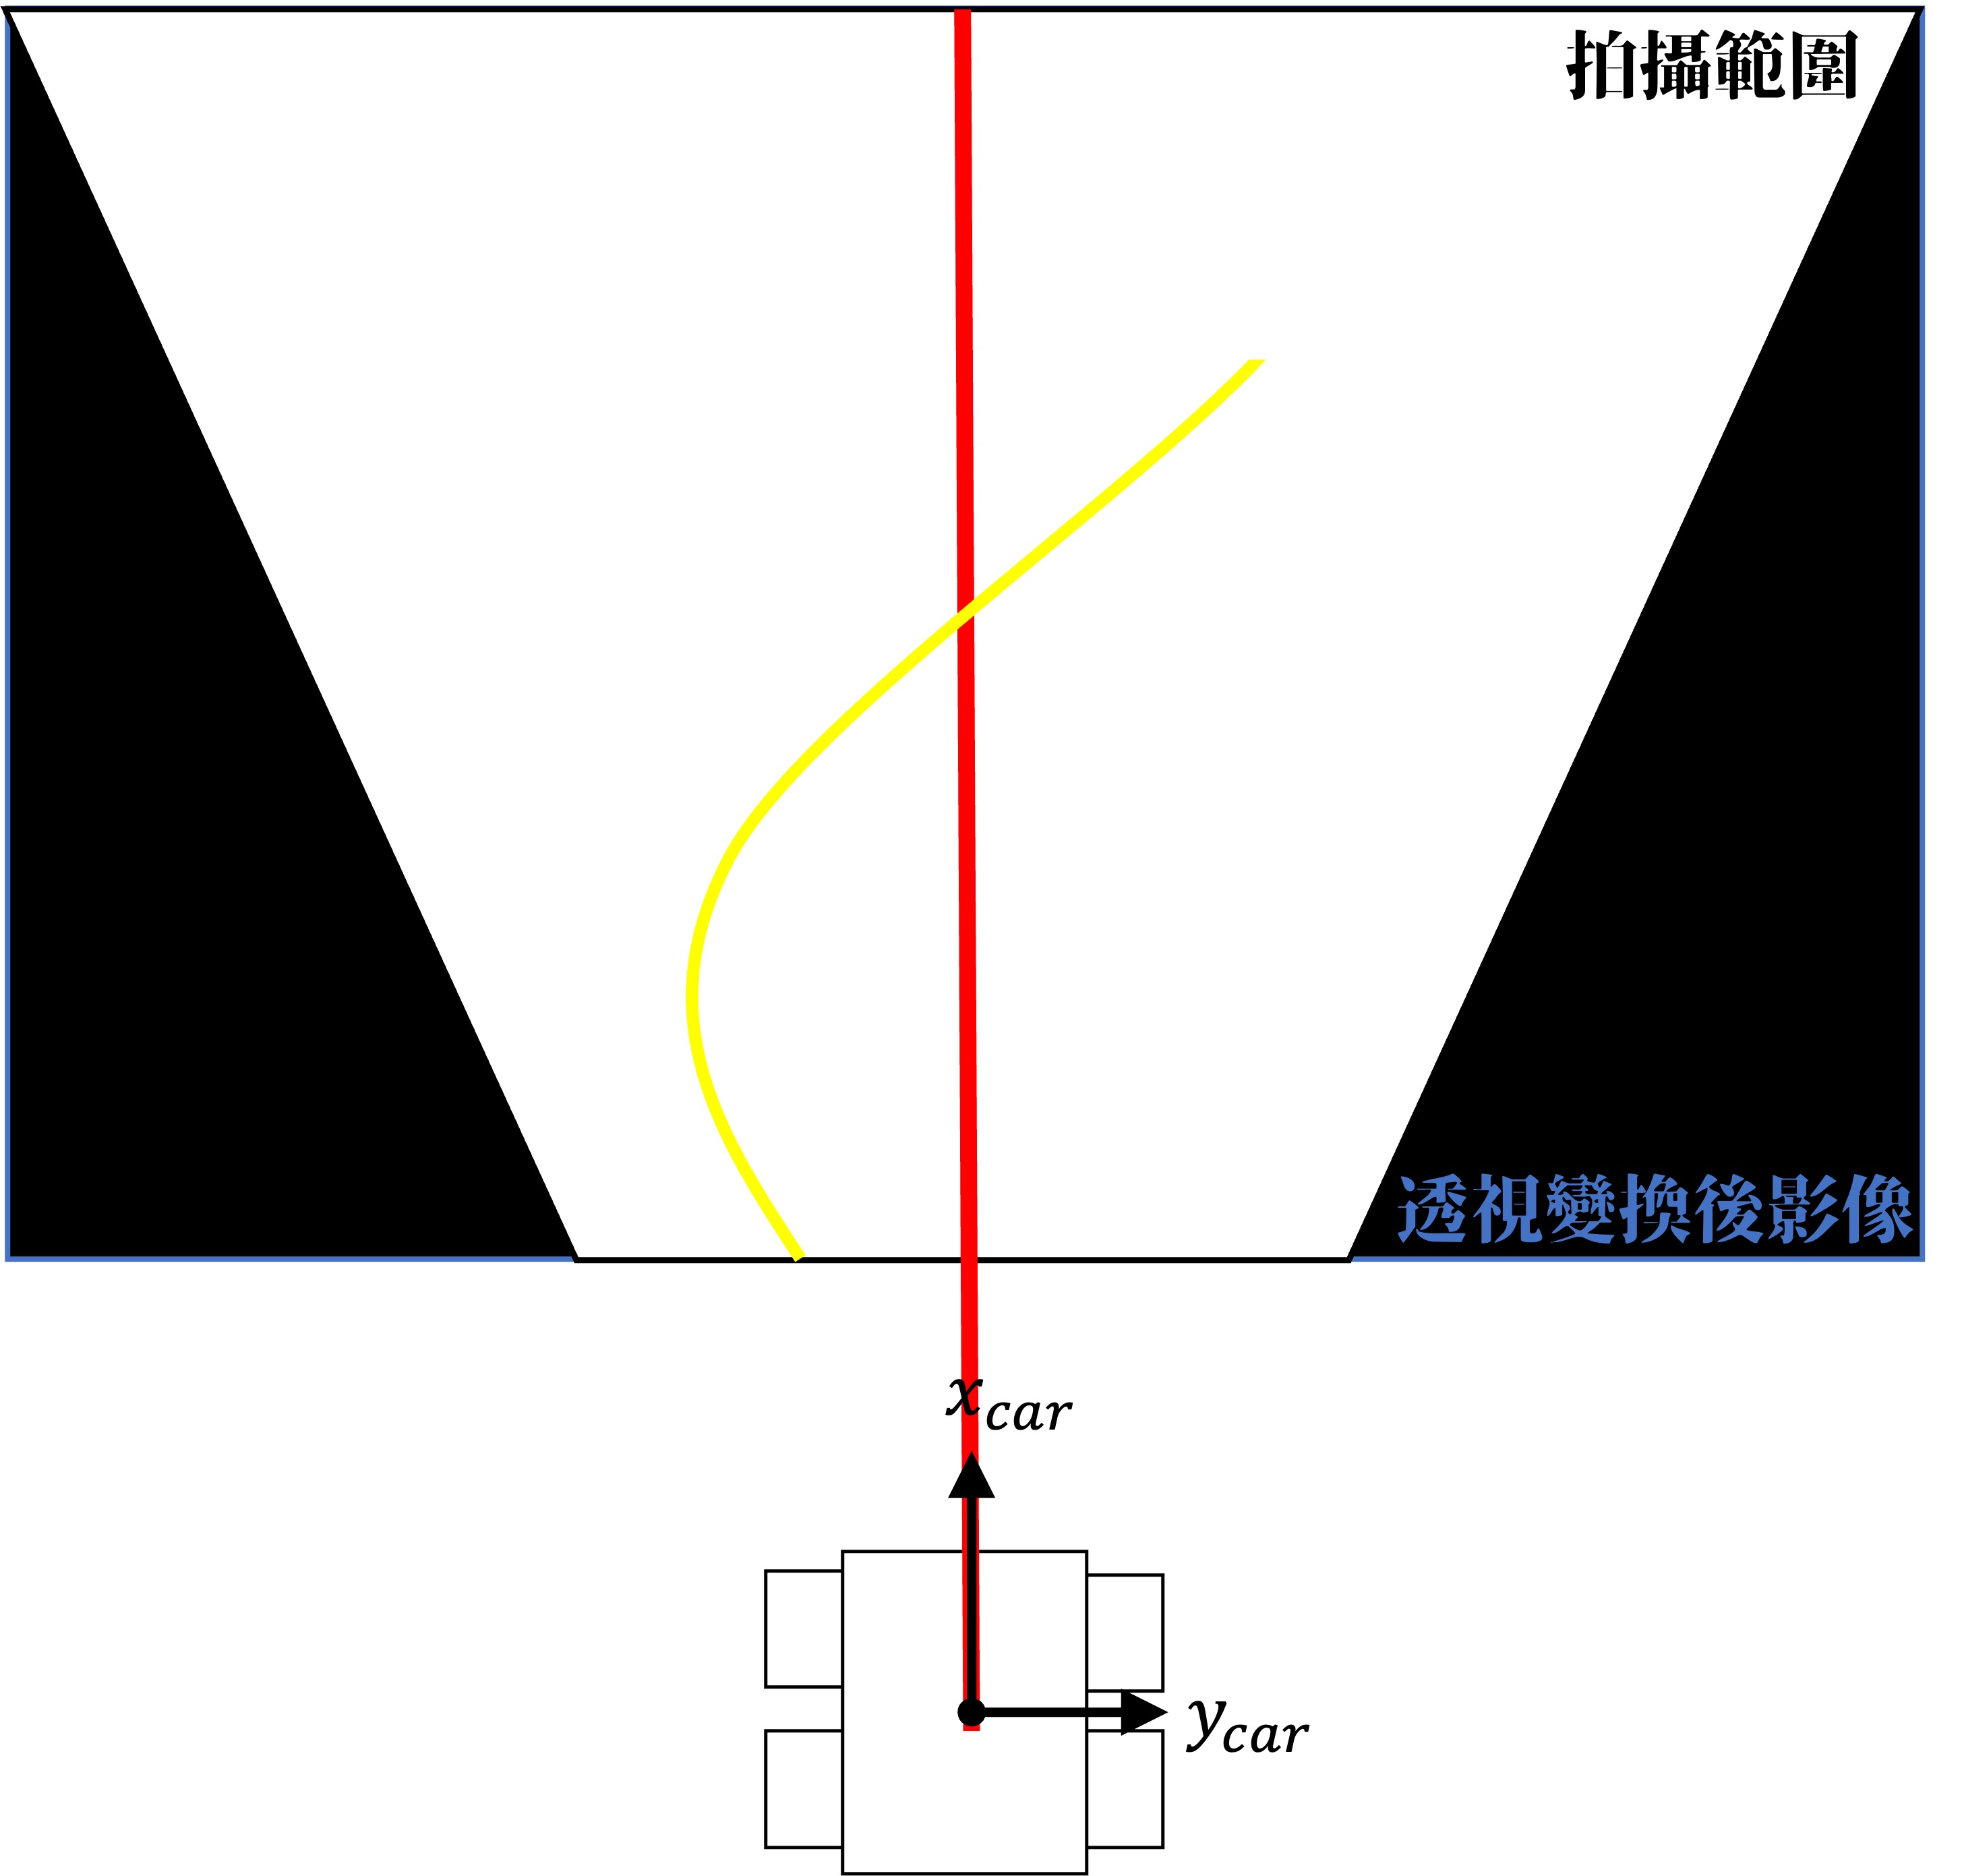
\includegraphics[width=0.7\textwidth]{19.jpg}     %圖片檔案名稱
    \caption{擬合後曲線與車輛座標系之$x$軸}    %圖片檔案名稱
    \label{fig:19}    %為圖片添加標籤
    %如\ref{fig:example1}所示
\end{figure}
根據擬合的曲線，計算出車輛當前的偏移量（與目標軌跡的水平距離）和偏移角度（與車道或目標方向的夾角）。這些數據將作為車輛調整行駛路徑的依據。
%==============================內文==============================

\subsubsection{模糊控制}
%==============================內文==============================
首先定義輸入變數與輸出變數。輸入變數為偏差角度$angle(\theta)$及位置偏移量$distance(mm)$。輸入變數為前進速度$V_{x}$、側向數度$V_{y}$與角速度$\omega$ 。

首先定義偏差角度$angle(\theta)$及位置偏移量$distance(mm)$的隸屬函數。

在本系統中，輸入變數包含偏差角度 $angle(\theta)$ 與位置偏移量 $distance$（mm），需先將其模糊化處理。其定義如下：

\begin{align}
    \theta &\in [-30^\circ, 30^\circ], \quad \theta \in \text{angle} = \{ \text{BL}, \text{SL}, \text{Z}, \text{SR}, \text{BR} \} \\
    d &\in [-50\,\text{mm}, 50\,\text{mm}], \quad distance \in \text{position} = \{ \text{BL}, \text{SL}, \text{Z}, \text{SR}, \text{BR} \}
\end{align}

上述模糊集合分別表示：
\begin{itemize}
    \item BL：大左 (Big Left)
    \item SL：小左 (Small Left)
    \item Z：居中 (Zero)
    \item SR：小右 (Small Right)
    \item BR：大右 (Big Right)
\end{itemize}

每個模糊集合都有對應的隸屬函數 $\mu_A(x)$，其映射如下：

\begin{equation}
    \mu_A(x) : X \rightarrow [0, 1]
\end{equation}


偏差角度$angle(\theta)$的隸屬函數如下：
\begin{align}
    \text{angle}_{\text{BL}}(x) = 
    \begin{cases}
    1 & x \le -25 \\
    \frac{x + 25}{15} & -25 < x \le -15 \\
    0 & \text{otherwise}
    \end{cases}    
\end{align}

\begin{align}
    \text{angle}_{\text{SL}}(x) = 
    \begin{cases}
    \frac{x + 25}{15} & -25 < x \le -15 \\
    \frac{-x}{10} & -15 < x \le 0 \\
    0 & \text{otherwise}
    \end{cases}    
\end{align}

\begin{align}
    \text{angle}_{Z}(x) = 
    \begin{cases}
    \frac{x + 5}{5} & -15 < x \le 0 \\
    \frac{5 - x}{5} & 0 < x \le 15 \\
    0 & \text{otherwise}
    \end{cases}    
\end{align}

\begin{align}
    \text{angle}_{\text{SR}}(x) = 
    \begin{cases}
    \frac{x}{15} & 0 < x \le 15 \\
    \frac{25 - x}{10} & 15 < x \le 25 \\
    0 & \text{otherwise}
    \end{cases}    
\end{align}

\begin{align}
    \text{angle}_{\text{BR}}(x) = 
    \begin{cases}
    \frac{x - 15}{15} & 15 < x \le 25 \\
    1 & x \ge 25 \\
    0 & \text{otherwise}
    \end{cases}    
\end{align}

\begin{figure}[H]
    \centering
    
\includegraphics[width=0.7\textwidth]{20.jpg}     %圖片檔案名稱
    \caption{偏差角度$angle(\theta)$隸屬函數}    %圖片檔案名稱
    \label{fig:20}    %為圖片添加標籤
    %如\ref{fig:example1}所示
\end{figure}

位置偏移量$distance(mm)$的隸屬函數如下：

\begin{align}
    \text{distance}_{\text{BL}}(x) = 
    \begin{cases}
    1 & x \le -35 \\
    \frac{x + 35}{10} & -35 < x \le -25 \\
    0 & \text{otherwise}
    \end{cases}    
\end{align}

\begin{align}
    \text{distance}_{\text{SL}}(x) = 
    \begin{cases}
    \frac{x + 35}{10} & -35 < x \le -25 \\
    \frac{-x}{25} & -25 < x \le 0 \\
    0 & \text{otherwise}
    \end{cases}    
\end{align}

\begin{align}
    \text{distance}_{Z}(x) = 
    \begin{cases}
    \frac{x + 10}{10} & -10 < x \le 0 \\
    \frac{10 - x}{10} & 0 < x \le 10 \\
    0 & \text{otherwise}
    \end{cases}    
\end{align}

\begin{align}
    \text{distance}_{\text{SR}}(x) = 
    \begin{cases}
    \frac{x}{20} & 0 < x \le 20 \\
    \frac{35 - x}{15} & 20 < x \le 35 \\
    0 & \text{otherwise}
    \end{cases}    
\end{align}

\begin{align}
    \text{distance}_{\text{BR}}(x) = 
    \begin{cases}
    \frac{x - 20}{15} & 20 < x \le 35 \\
    1 & x \ge 35 \\
    0 & \text{otherwise}
    \end{cases}    
\end{align}

\begin{figure}[H]
    \centering
    
\includegraphics[width=0.7\textwidth]{21.jpg}     %圖片檔案名稱
    \caption{位置偏移量$distance(mm)$隸屬函數}    %圖片檔案名稱
    \label{fig:21}    %為圖片添加標籤
    %如\ref{fig:example1}所示
\end{figure}

接著定義前進速度$V_{x}$、側向數度$V_{y}$與角速度$\omega$的隸屬函數。

前進速度$V_{x}$定義為：
\begin{itemize}
    \item S (Slow)：慢速
    \item M (Medium)：中速
    \item F (Fast)：快速
\end{itemize}

前進速度$V_{x}$的隸屬函數如下：
\begin{align}
    \text{Vx}_{S}(x) = 
    \begin{cases}
    1 & 0 \le x \le 50 \\
    \frac{80- x}{30} & 50 < x \le 80 \\
    0 & \text{otherwise}
    \end{cases}
\end{align}

\begin{align}
    \text{Vx}_{M}(x) = 
    \begin{cases}
    \frac{x - 50}{30} & 50 < x \le 80 \\
    \frac{150 - x}{70} & 80 < x \le 150 \\
    0 & \text{otherwise}
    \end{cases}
\end{align}

\begin{align}
    \text{Vx}_{F}(x) = 
    \begin{cases}
    \frac{x - 80}{70} & 80 < x \le 150 \\
    1 & 150 < x \le 150 \\
    0 & \text{otherwise}
    \end{cases}    
\end{align}

\begin{figure}[H]
    \centering
    
\includegraphics[width=0.8\textwidth]{22.jpg}     %圖片檔案名稱
    \caption{前進速度$V_{x}$隸屬函數}    %圖片檔案名稱
    \label{fig:22}    %為圖片添加標籤
    %如\ref{fig:example1}所示
\end{figure}

側向數度$V_{y}$定義為：
\begin{itemize}
    \item LL (Leftmost)：最左
    \item L (Left)：左
    \item Z (Zero)：中間
    \item R (Right)：右
    \item RR (Rightmost)：最右
\end{itemize}

側向數度$V_{y}$的隸屬函數如下：

\begin{align}
    \text{Vy}_{LL}(x) = 
    \begin{cases}
    1 & -30 \le x \le -20 \\
    \frac{-12 - x}{8} & -20 < x \le -12 \\
    0 & \text{otherwise}
    \end{cases}       
\end{align}

\begin{align}
    \text{Vy}_{L}(x) = 
    \begin{cases}
    \frac{x + 16}{4} & -16 < x \le -12 \\
    \frac{-x}{12} & -12 < x \le 0 \\
    0 & \text{otherwise}
    \end{cases}    
\end{align}

\begin{align}
    \text{Vy}_{Z}(x) = 
    \begin{cases}
    \frac{x + 14}{14} & -14 < x \le 0 \\
    \frac{14 - x}{14} & 0 < x \le 14 \\
    0 & \text{otherwise}
    \end{cases}     
\end{align}

\begin{align}
    \text{Vy}_{R}(x) = 
    \begin{cases}
    \frac{x}{12} & 0 < x \le 12 \\
    \frac{16 - x}{4} & 12 < x \le 16 \\
    0 & \text{otherwise}
    \end{cases}     
\end{align}

\begin{align}
    \text{Vy}_{RR}(x) = 
    \begin{cases}
    \frac{x - 12}{8} & 12 < x \le 20 \\
    1 & 20 < x \le 30 \\
    0 & \text{otherwise}
    \end{cases}       
\end{align}

\begin{figure}[H]
    \centering
    
\includegraphics[width=0.8\textwidth]{23.jpg}     %圖片檔案名稱
    \caption{側向數度$V_{y}$隸屬函數}    %圖片檔案名稱
    \label{fig:23}    %為圖片添加標籤
    %如\ref{fig:example1}所示
\end{figure}

角速度$\omega$定義為：
\begin{itemize}
    \item CCW2 (Counterclockwise 2)：強烈逆時針
    \item CCW (Counterclockwise)：輕微逆時針
    \item Z (Zero)：無旋轉
    \item CW (Clockwise)：輕微順時針
    \item CW2 (Clockwise 2)：強烈順時針
\end{itemize}
角速度$\omega$的隸屬函數如下：

\begin{align}
    \omega_{\text{CCW2}}(x) = 
    \begin{cases}
    1 & -20 \le x \le -10 \\
    \frac{-10 - x}{2} & -10 < x \le -8 \\
    0 & \text{otherwise}
    \end{cases}    
\end{align}

\begin{align}
    \omega_{\text{CCW}}(x) = 
    \begin{cases}
    \frac{x + 10}{6} & -10 < x \le -4 \\
    \frac{-x}{4} & -4 < x \le 0 \\
    0 & \text{otherwise}
    \end{cases}     
\end{align}

\begin{align}
    \omega_{Z}(x) = 
    \begin{cases}
    \frac{x + 4}{4} & -4 < x \le 0 \\
    \frac{4 - x}{4} & 0 < x \le 4 \\
    0 & \text{otherwise}
    \end{cases}    
\end{align}

\begin{align}
    \omega_{\text{CW}}(x) = 
    \begin{cases}
    \frac{x}{10} & 0 < x \le 4 \\
    \frac{10 - x}{6} & 4 < x \le 10 \\
    0 & \text{otherwise}
    \end{cases}      
\end{align}

\begin{align}
    \omega_{\text{CW2}}(x) = 
    \begin{cases}
    \frac{x - 8}{2} &  8< x \le 10 \\
    1 & 10 < x \le 20 \\
    0 & \text{otherwise}
    \end{cases}      
\end{align}

\begin{figure}[H]
    \centering
    
\includegraphics[width=0.8\textwidth]{24.jpg}     %圖片檔案名稱
    \caption{角速度$\omega$隸屬函數}    %圖片檔案名稱
    \label{fig:24}    %為圖片添加標籤
    %如\ref{fig:example1}所示
\end{figure}

接著是定義控制規則庫，$V_{x}$之控制規則表、$V_{y}$控制規則表與$\omega$控制規則表，如下所示。

\begin{table}[H]
    \centering
    \caption{$V_{x}$控制規則表}
    \vspace{6pt} % 增加空格
    \begin{tabular}{|c|c|c|c|c|c|}
    \hline
    \diagbox{\textbf{Angle($^\circ$)}}{\textbf{Position(cm)}} & \textbf{BL} & \textbf{SL} & \textbf{Z} & \textbf{SR} & \textbf{BR} \\
    \hline
    \textbf{BL} & S & S & M & S & S \\
    \hline
    \textbf{SL} & S & M & F & M & S \\
    \hline
    \textbf{Z} & M & F & F & F & M \\
    \hline
    \textbf{SR} & S & M & F & M & S \\
    \hline
    \textbf{BR} & S & S & M & S & S \\
    \hline
    \end{tabular}
    \label{tab:fu1}
\end{table}

\begin{table}[H]
    \centering
    \caption{$V_{y}$控制規則表}
    \vspace{6pt} % 增加空格
    \begin{tabular}{|c|c|c|c|c|c|}
    \hline
    \diagbox{\textbf{Angle($^\circ$)}}{\textbf{Position(cm)}}& \textbf{BL} & \textbf{SL} & \textbf{Z} & \textbf{SR} & \textbf{BR} \\
    \hline
    \textbf{BL} & RR & R & Z & L & LL \\
    \hline
    \textbf{SL} & RR & R & Z & L & LL \\
    \hline
    \textbf{Z} & RR & R & Z & L & LL \\
    \hline
    \textbf{SR} & RR & R & Z & L & LL \\
    \hline
    \textbf{BR} & RR & R & Z & L & LL \\
    \hline
    \end{tabular}
    \label{tab:fu2}
\end{table}

\begin{table}[H]
    \centering
    \caption{$\omega$控制規則表}
    \vspace{6pt} % 增加空格
    \begin{tabular}{|c|c|c|c|c|c|}
    \hline
    \diagbox{\textbf{Angle($^\circ$)}}{\textbf{Position(cm)}}& \textbf{BL} & \textbf{SL} & \textbf{Z} & \textbf{SR} & \textbf{BR} \\
    \hline
    \textbf{BL} & CW2 & CW2 & CW2 & CW2 & CW2 \\
    \hline
    \textbf{SL} & CW & CW & CW & CW & CW \\
    \hline
    \textbf{Z} & Z & Z & Z & Z & Z \\
    \hline
    \textbf{SR} & CCW & CCW & CCW & CCW & CCW2 \\
    \hline
    \textbf{BR} & CCW2 & CCW2 & CCW2 & CCW2 & CCW2 \\
    \hline
    \end{tabular}
    \label{tab:fu3}
\end{table}
觸發強度是由這兩個模糊集合的隸屬度中的較小者所決定。
\begin{align}
        \alpha_{ij} = \min\left( \mu^{A_i}_{\text{angle}}(\theta),\ \mu^{B_j}_{\text{position}}(x) \right)
\end{align}

最後進行去模糊化，計算對每個輸出變數$z$，計算：

\begin{align}
    z^* = \frac{\int z \cdot \mu(z) \, dz}{\int \mu(z) \, dz}    
\end{align}

其中，$\mu(z)$是合併後的輸出模糊集合的隸屬度。

因為有數組輸出，利用Alpha-Cut（$\alpha$-截集）的方式，排除異常值，僅保留後 80\% 結果來避免極端值干擾。

對輸出值集合${z_i}$，排序後選取前$N \times \alpha$個，再取平均：
\begin{align}
    \bar{z}_\alpha = \frac{1}{N_\alpha} \sum_{i=1}^{N_\alpha} z_i 
\end{align}

最後即可取得不同偏差角度$angle$及位置偏移量$distance$對應之前進速度$V_{x}$(圖\ref{fig:25})、側向數度$V_{y}$(圖\ref{fig:26})與角速度$\omega$(圖\ref{fig:27})。

\begin{figure}[H]
    \centering
    
\includegraphics[width=0.8\textwidth]{25.jpg}     %圖片檔案名稱
    \caption{不同偏差角度及偏移量對應之前進速度$V_{x}$}    %圖片檔案名稱
    \label{fig:25}    %為圖片添加標籤
    %如\ref{fig:example1}所示
\end{figure}

\begin{figure}[H]
    \centering
    
\includegraphics[width=0.8\textwidth]{26.jpg}     %圖片檔案名稱
    \caption{不同偏差角度及偏移量對應之側向數度$V_{y}$}    %圖片檔案名稱
    \label{fig:26}    %為圖片添加標籤
    %如\ref{fig:example1}所示
\end{figure}

\begin{figure}[H]
    \centering
    
\includegraphics[width=0.8\textwidth]{27.jpg}     %圖片檔案名稱
    \caption{不同偏差角度及偏移量對應之角速度$\omega$}    %圖片檔案名稱
    \label{fig:27}    %為圖片添加標籤
    %如\ref{fig:example1}所示
\end{figure}
%==============================內文==============================

\section{\centering 模擬與分析}

\subsection{影像偵測演算法模擬} 
%==============================內文==============================
\hspace{2em}首先是進行影像透視變換實際測試，並利用逆透視變換取得影像中特定像素點在以車輛為原點的平面座標系之座標。

影像透視變換測試結果如圖\ref{fig:36}所示。將實際拍攝影像投影至以車輛為原點的平面上，即可計算拍攝目標物與車輛之距離，圖中座標單位為公尺。
\begin{figure}[H]
    \centering
    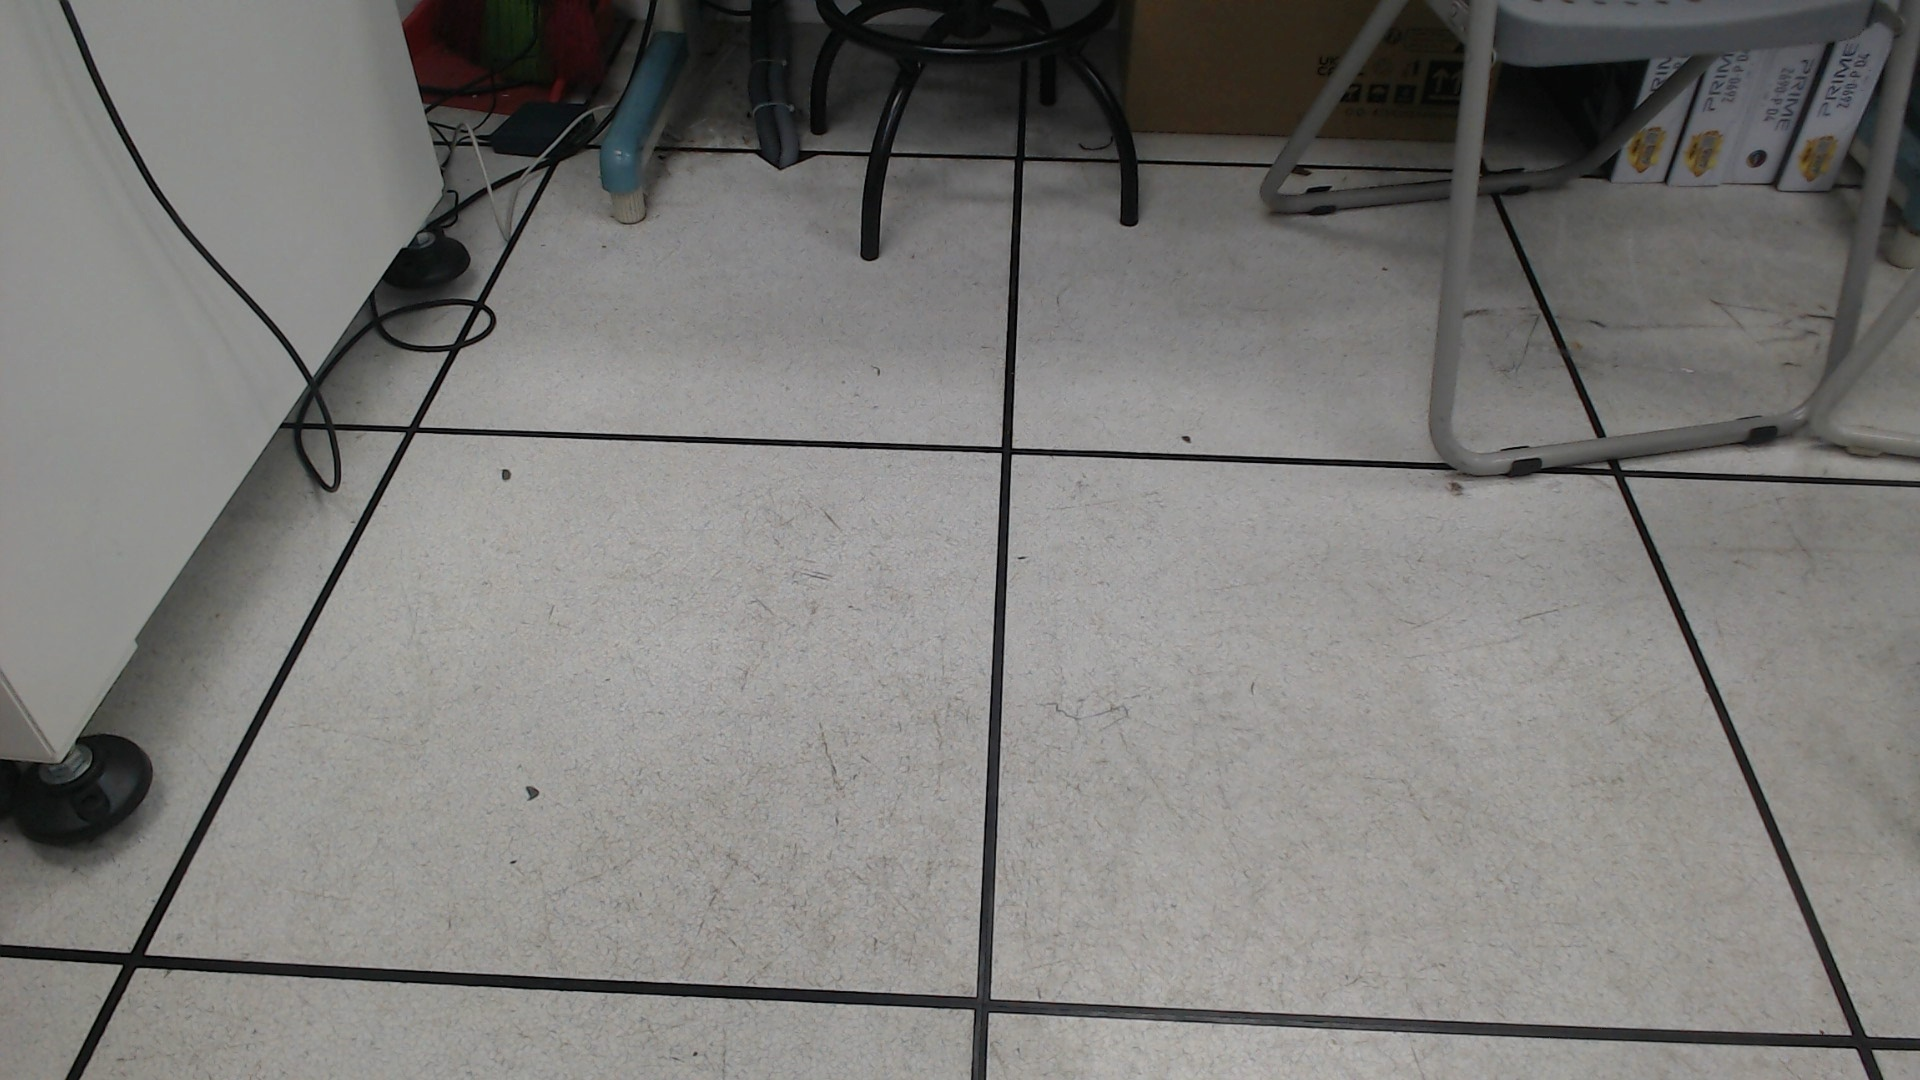
\includegraphics[width=0.7\textwidth]{35.jpg}     %圖片檔案名稱
    \caption{尚未進行透視變換之原始圖片}    %圖片檔案名稱
    \label{fig:35}    %為圖片添加標籤
    %如\ref{fig:MxzONoG}所示
\end{figure}
\begin{figure}[H]
    \centering
    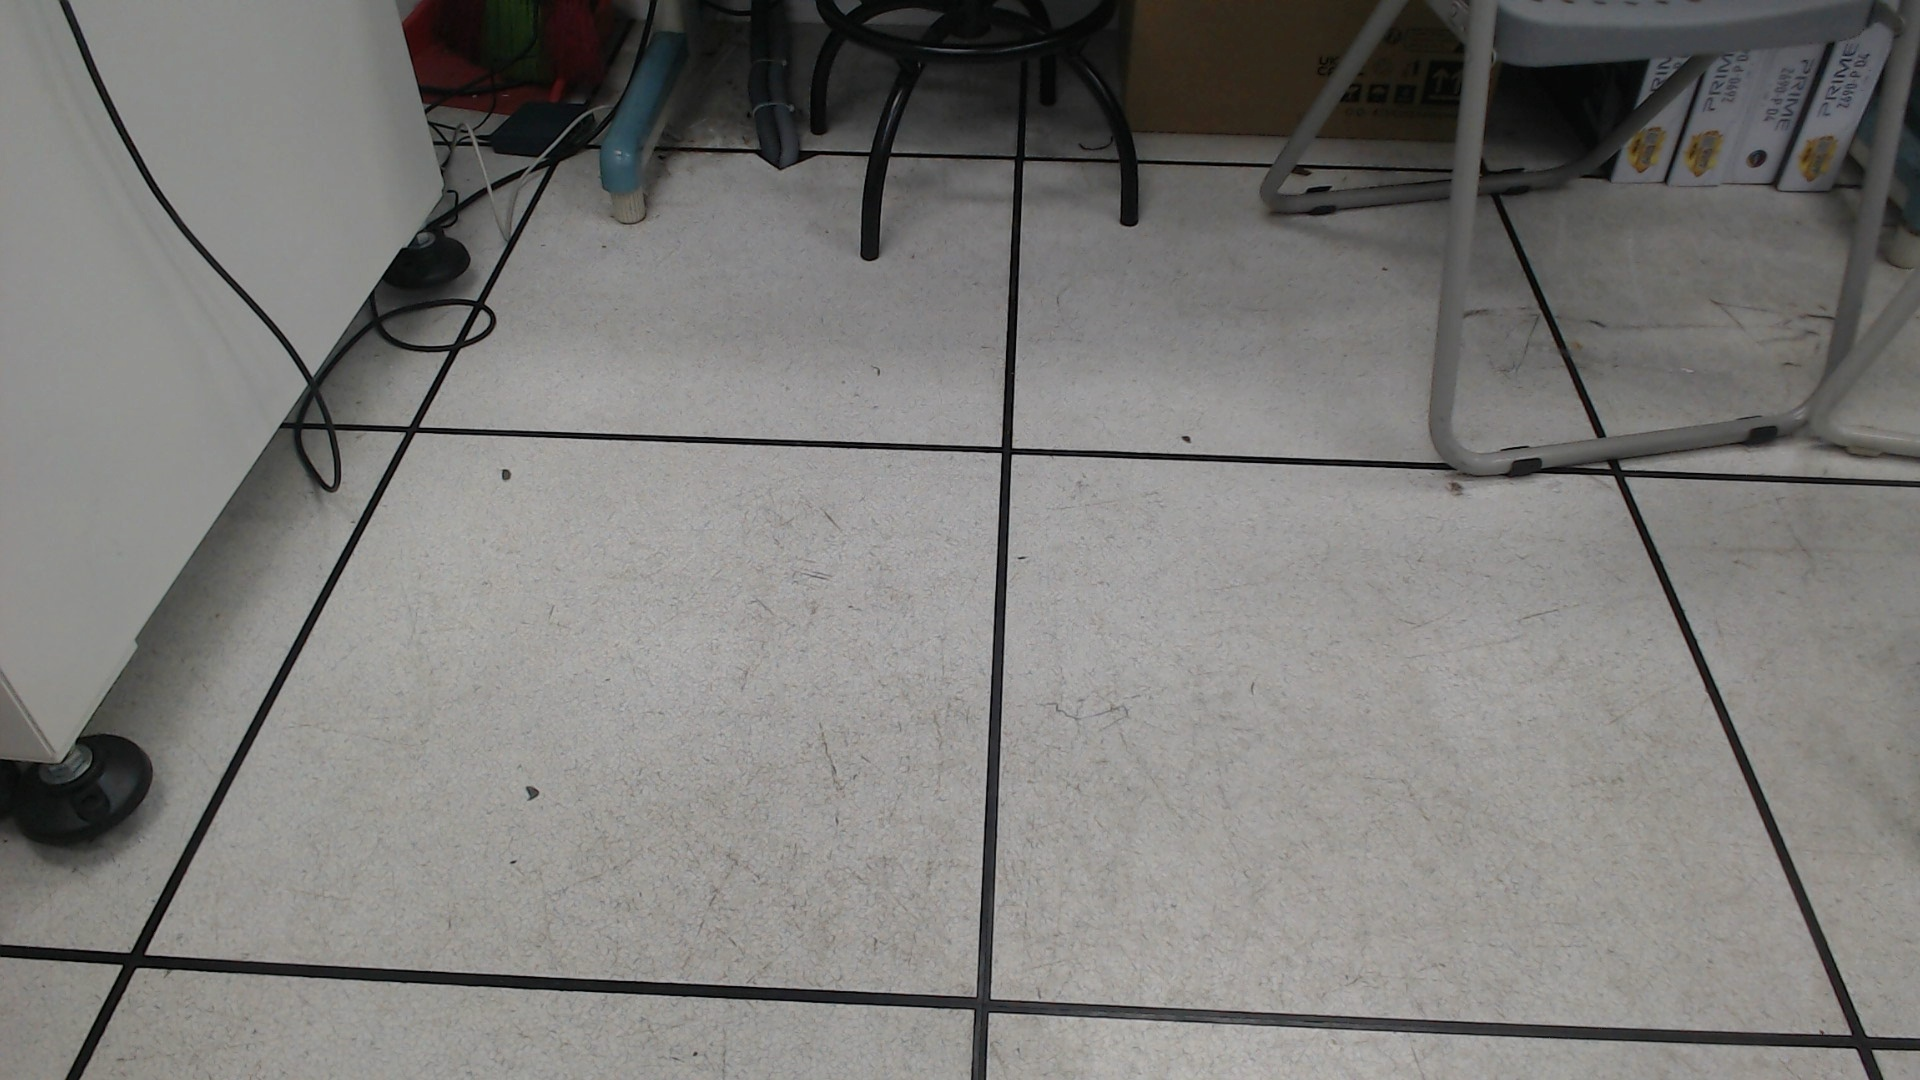
\includegraphics[width=0.7\textwidth]{35.jpg}     %圖片檔案名稱
    \caption{經透視變換後影像}    %圖片檔案名稱
    \label{fig:36}    %為圖片添加標籤
    %如\ref{fig:MxzONoG}所示
\end{figure}

下圖(如圖\ref{fig:frame_with_points_real}所示)與下表(如表\ref{tab:error_comparison}所示)為逆透視變換之結果，
與計算之誤差，可知若參數設置準確，絕對誤差大約為7mm左右，且測試時相機距離地面1.5公尺。若離地面更近，絕對誤差理論上會更小。

\begin{figure}[H]
    \centering
    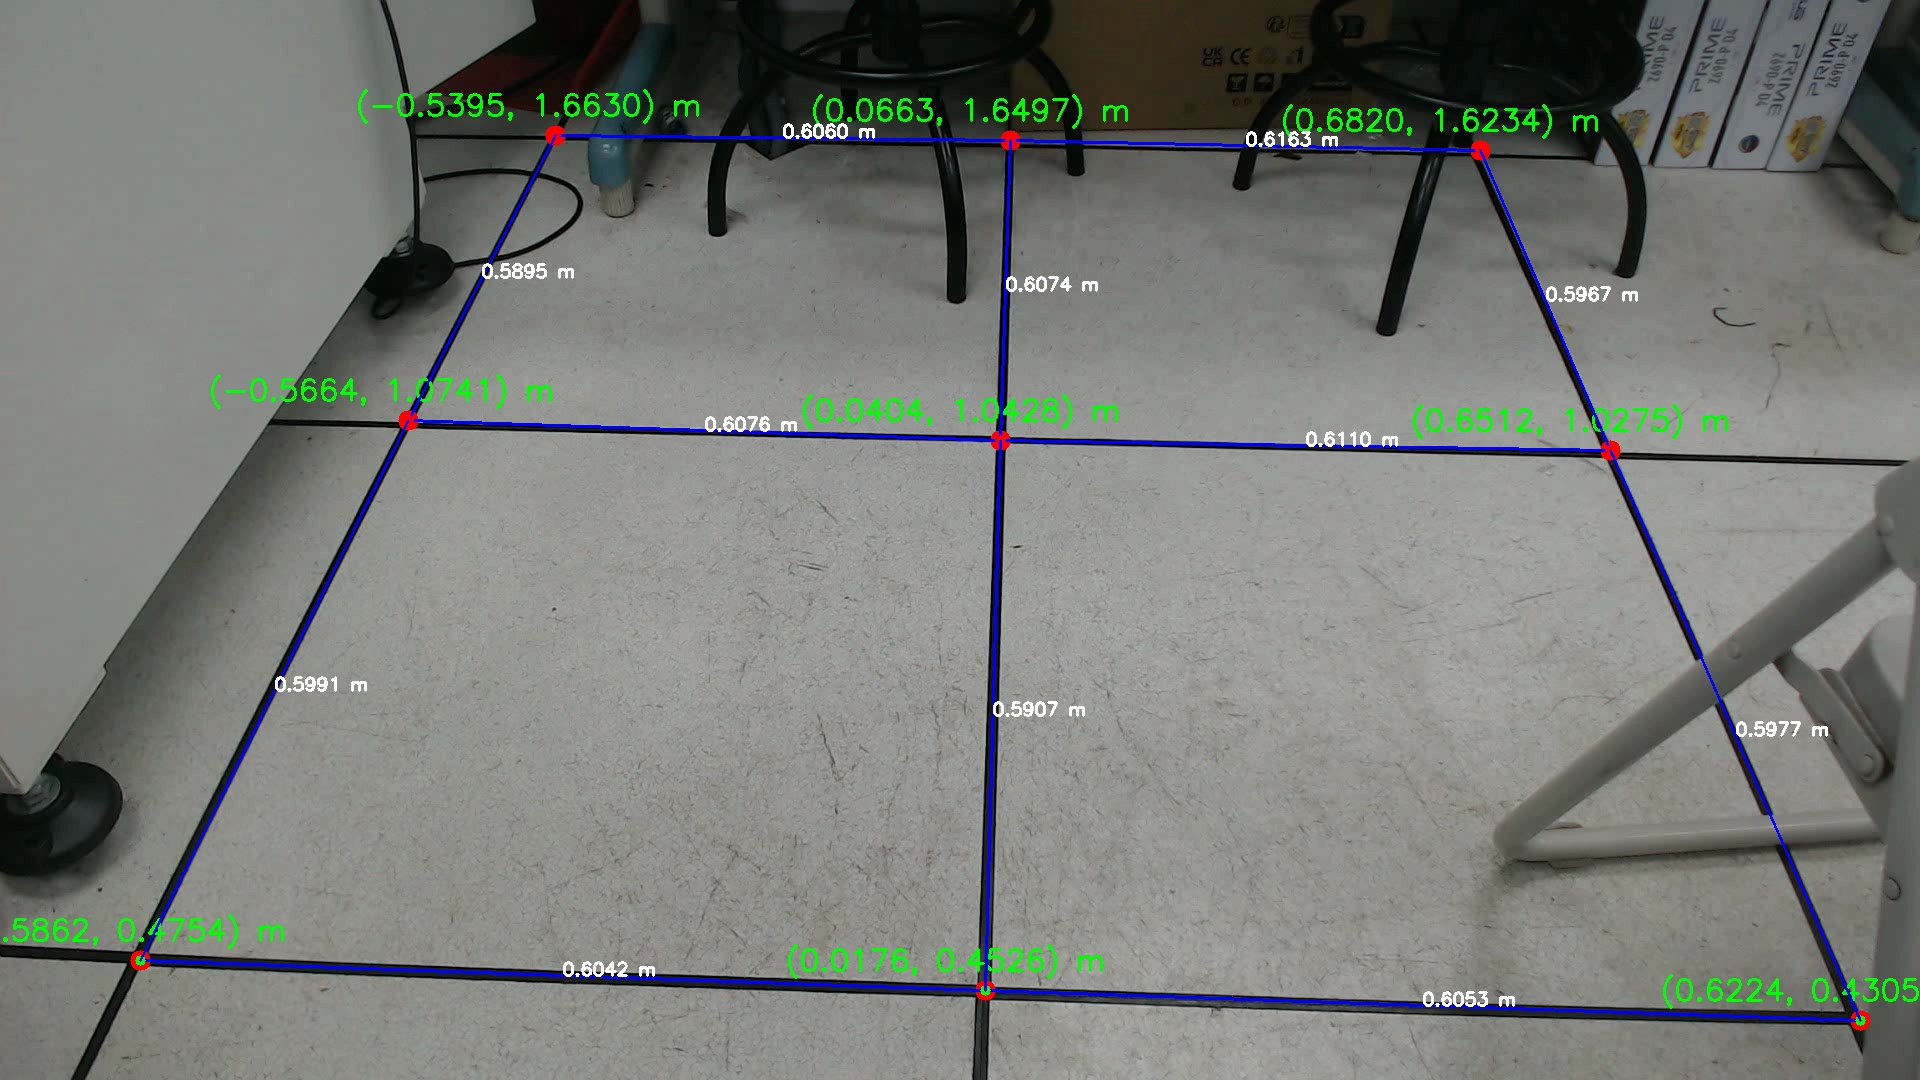
\includegraphics[width=0.7\textwidth]{frame_with_points_real.jpg}     %圖片檔案名稱
    \caption{實際測量地板尺寸}    %圖片檔案名稱
    \label{fig:frame_with_points_real}    %為圖片添加標籤
    %(如圖\ref{fig:frame_with_points_real}所示)
\end{figure}

\begin{table}[H]
    \centering
    \caption{透視變換誤差}
    \vspace{6pt} % 增加空格
    \label{tab:error_comparison}
    \begin{tabular}{lS[table-format=2.2]S[table-format=2.2]}
        \toprule
        MAE(m) & 0.007  \\
        MRE(\%) & 1.168 \\
        \bottomrule
    \end{tabular}
\end{table}

接下來是進行影像偵測之模擬，測試影像處理方式是否可行，先由行車圖片進行測試，圖\ref{fig:37}為原始圖片，圖\ref{fig:38}為經灰階處理之圖片，圖\ref{fig:38}為經高斯模糊處理之圖片。
\begin{figure}[H]
    \centering
    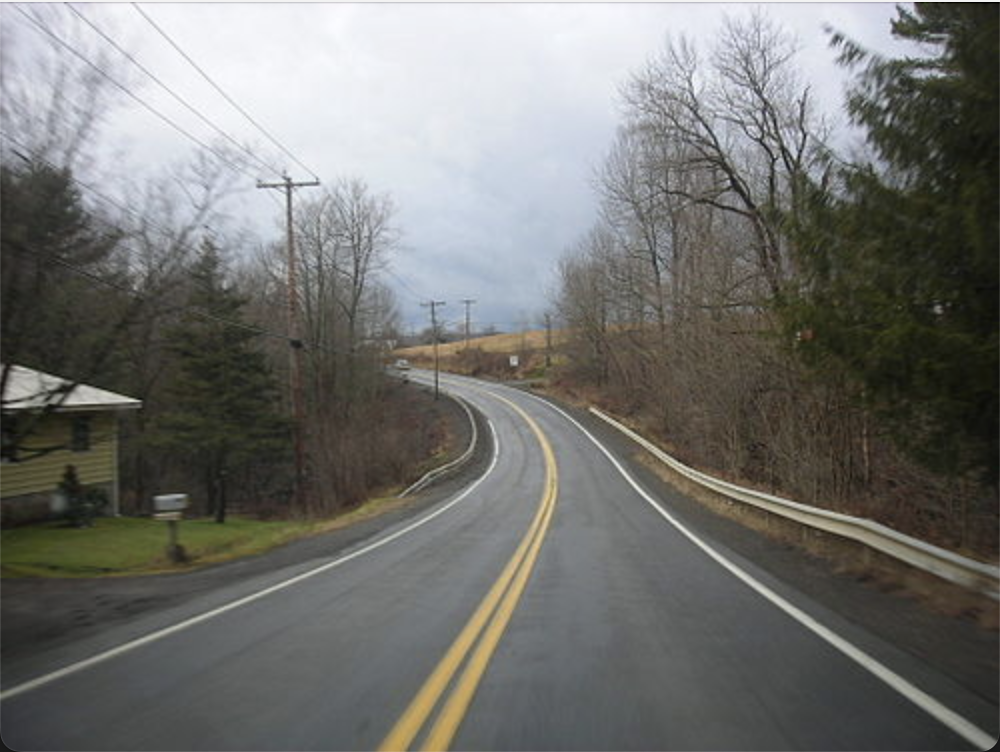
\includegraphics[width=0.7\textwidth]{37.jpg}     %圖片檔案名稱
    \caption{待測試之原始圖片}    %圖片檔案名稱
    \label{fig:37}    %為圖片添加標籤
    %如\ref{fig:MxzONoG}所示
\end{figure}

\begin{figure}[H]
    \centering
    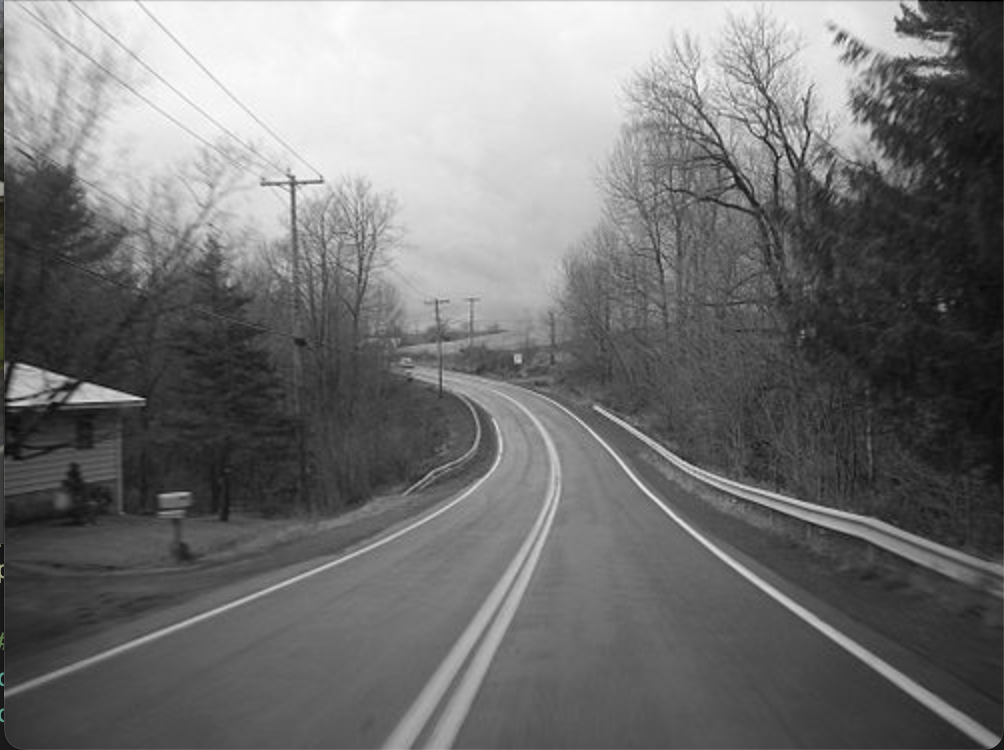
\includegraphics[width=0.7\textwidth]{38.jpg}     %圖片檔案名稱
    \caption{經灰階處理之圖片}    %圖片檔案名稱
    \label{fig:38}    %為圖片添加標籤
    %如\ref{fig:2}所示
\end{figure}

\begin{figure}[H]
    \centering
    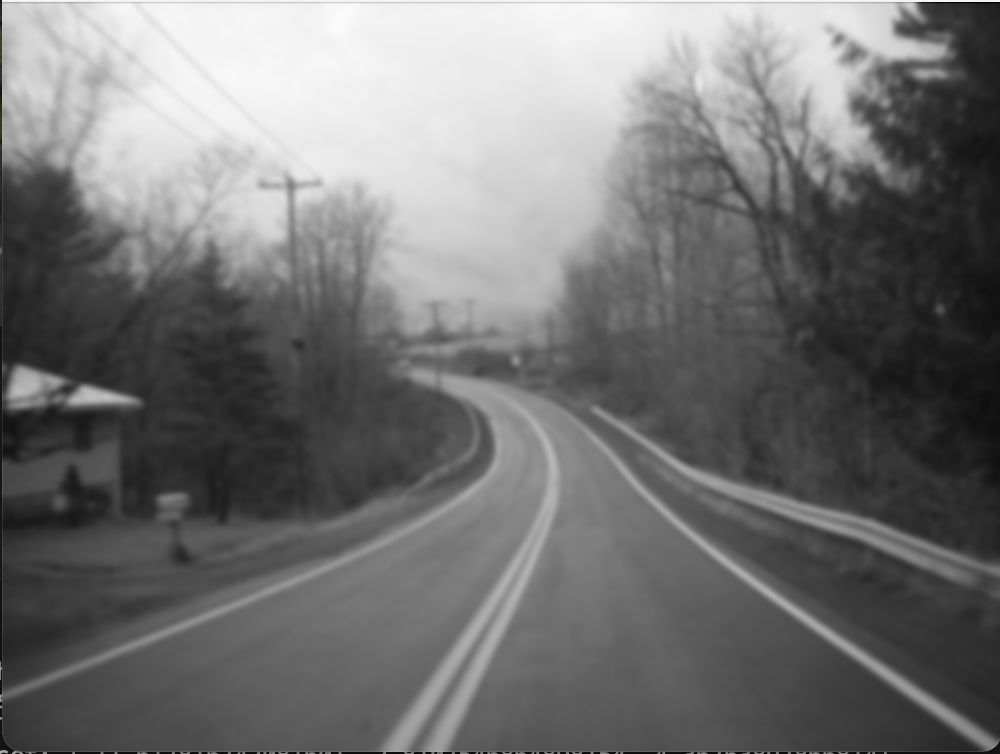
\includegraphics[width=0.7\textwidth]{39.jpg}     %圖片檔案名稱
    \caption{經高斯模糊處理之圖片}    %圖片檔案名稱
    \label{fig:39}    %為圖片添加標籤
    %如\ref{fig:2}所示
\end{figure}

圖\ref{fig:40}為經二值化處理之圖片，圖\ref{fig:41}為經邊緣偵測之圖片，
在偵測邊緣前會在經過一次高斯模糊，再次過濾二值化後產生的雜訊。

\begin{figure}[H]
    \centering
    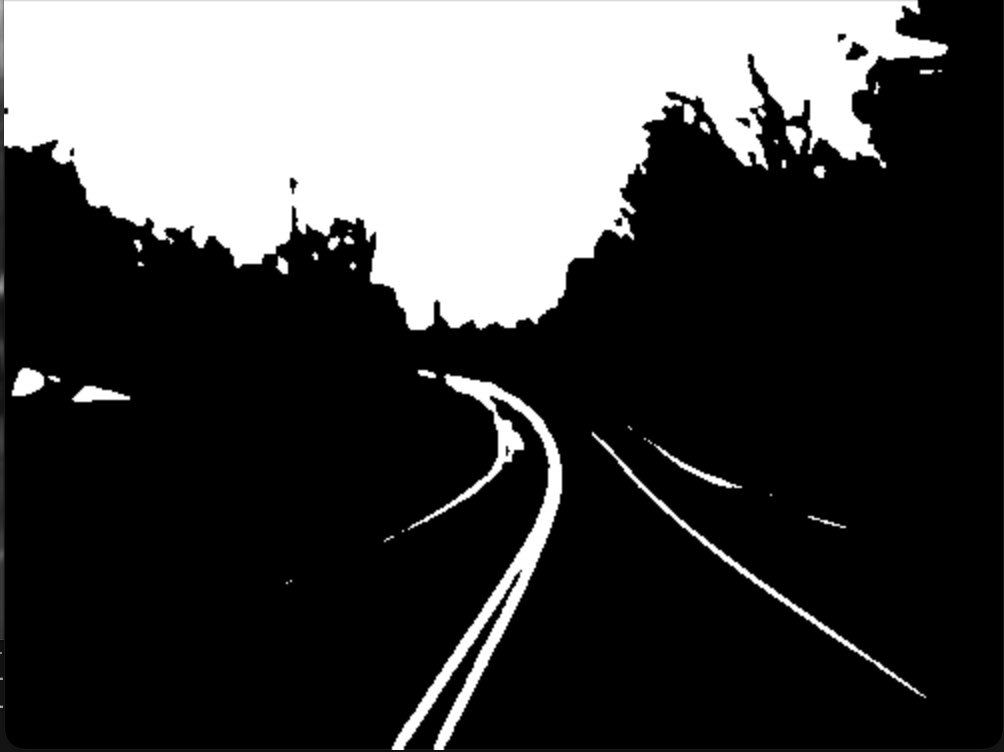
\includegraphics[width=0.7\textwidth]{40.jpg}     %圖片檔案名稱
    \caption{經二值化處理之圖片}    %圖片檔案名稱
    \label{fig:40}    %為圖片添加標籤
    %如\ref{fig:2}所示
\end{figure}

\begin{figure}[H]
    \centering
    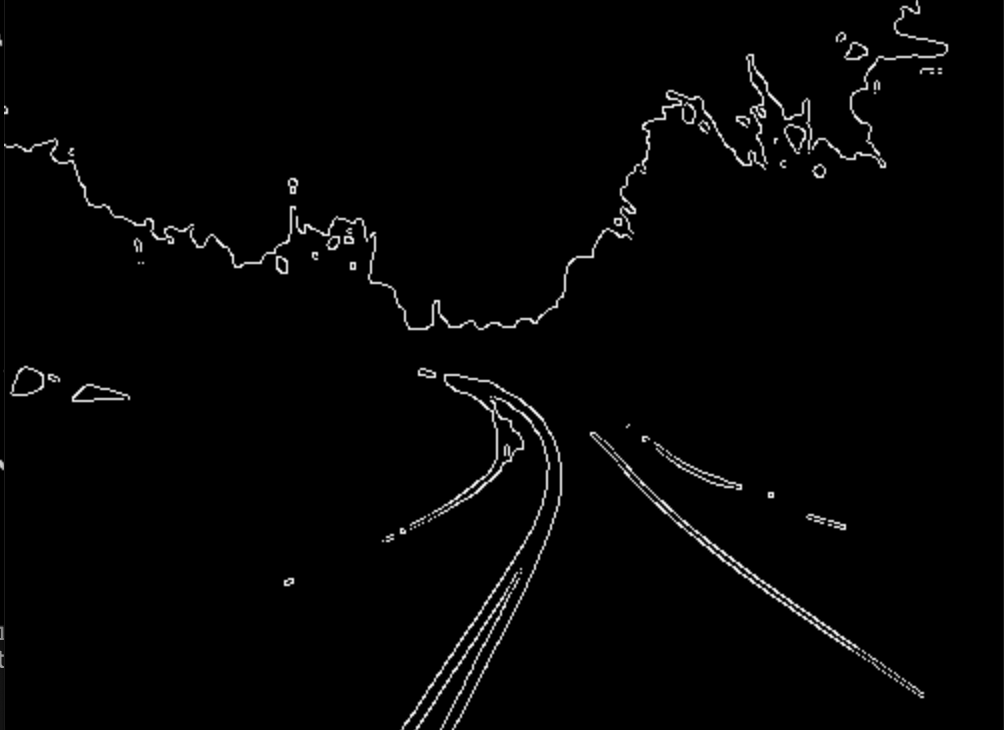
\includegraphics[width=0.7\textwidth]{41.jpg}     %圖片檔案名稱
    \caption{經邊緣偵測之圖片}    %圖片檔案名稱
    \label{fig:41}    %為圖片添加標籤
    %如\ref{fig:2}所示
\end{figure}

經過canny邊緣偵測後的圖片，只有黑白兩種像素，
標線邊緣為白色，其他均為黑色，因此可利用白色像素進行偵測。下圖為測試之結果。

\begin{figure}[H]
    \centering
    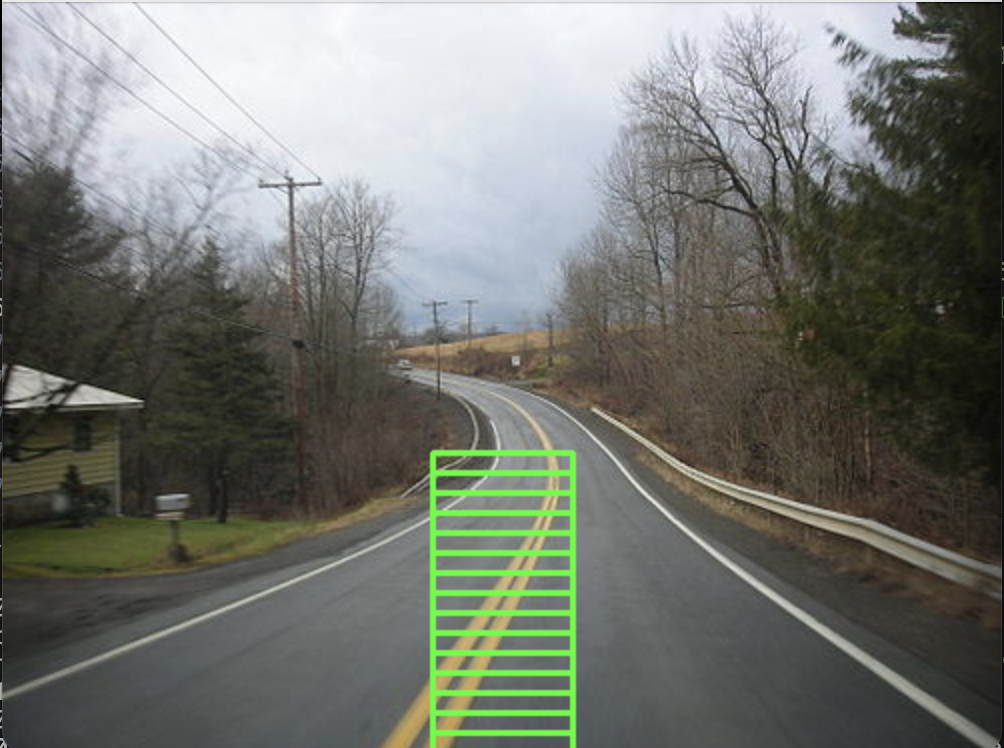
\includegraphics[width=0.7\textwidth]{42.jpg}     %圖片檔案名稱
    \caption{尚未滑動之偵測視窗}    %圖片檔案名稱
    \label{fig:42}    %為圖片添加標籤
    %如\ref{fig:2}所示
\end{figure}
\begin{figure}[H]
    \centering
    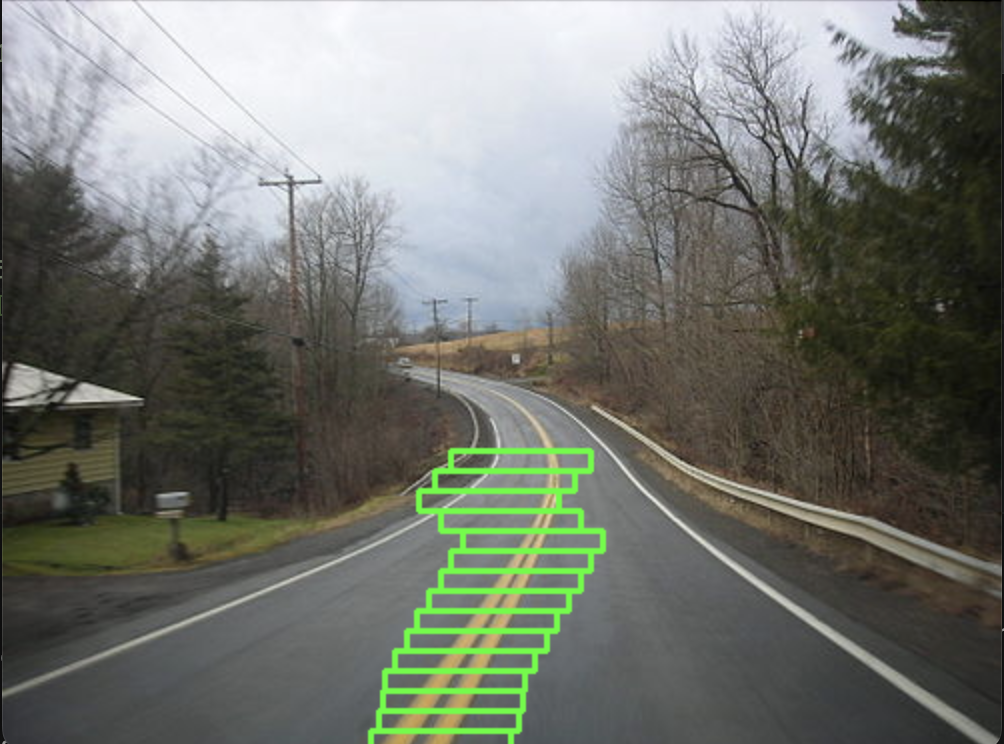
\includegraphics[width=0.7\textwidth]{43.jpg}     %圖片檔案名稱
    \caption{滑動後偵測視窗}    %圖片檔案名稱
    \label{fig:43}    %為圖片添加標籤
    %如\ref{fig:2}所示
\end{figure}

下圖為實際擬合曲線之結果，可見圖片下方的部分大致有擬合出來，但上方的標線有偏離目標標線的現象。

\begin{figure}[H]
    \centering
    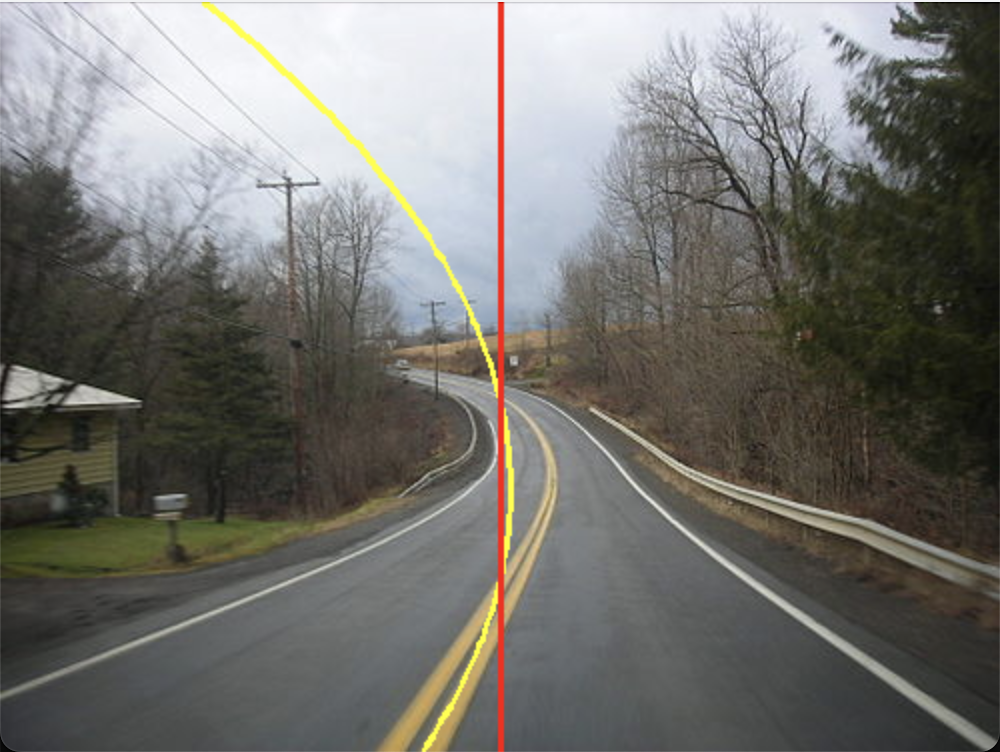
\includegraphics[width=0.7\textwidth]{44.jpg}     %圖片檔案名稱
    \caption{擬合後曲線與車輛行駛方向比較}    %圖片檔案名稱
    \label{fig:44}    %為圖片添加標籤
    %如\ref{fig:2}所示
\end{figure}

因為測試圖判沒有做透視變換處理，藉由觀察，
可看到為最頂端的幾個偵測視窗，有偵測到其他條線，因此有偏離目標的現象，最後擬合的曲線在那部分也相較下方沒有完全貼合目標。
由此可知透視變換之處理有其必要性。

經這幾項測試，判斷此影像處理及偵測方法可用於循線自走車。
%==============================內文==============================

\subsection{車輛模糊控制移動路徑模擬} 
%==============================內文==============================
\hspace{2em}在判斷此影像處理及偵測方法可用於循線自走車後，對模擬車輛經模糊控制後行進路進行分析。
此部分用Matlab撰寫了一個模擬環境，依照場地規格，畫出競賽場，如圖\ref{fig:00}所示，其中藍色線為標線，紅色線為界線，黑色匡為車體本身。

\begin{figure}[H]
    \centering
    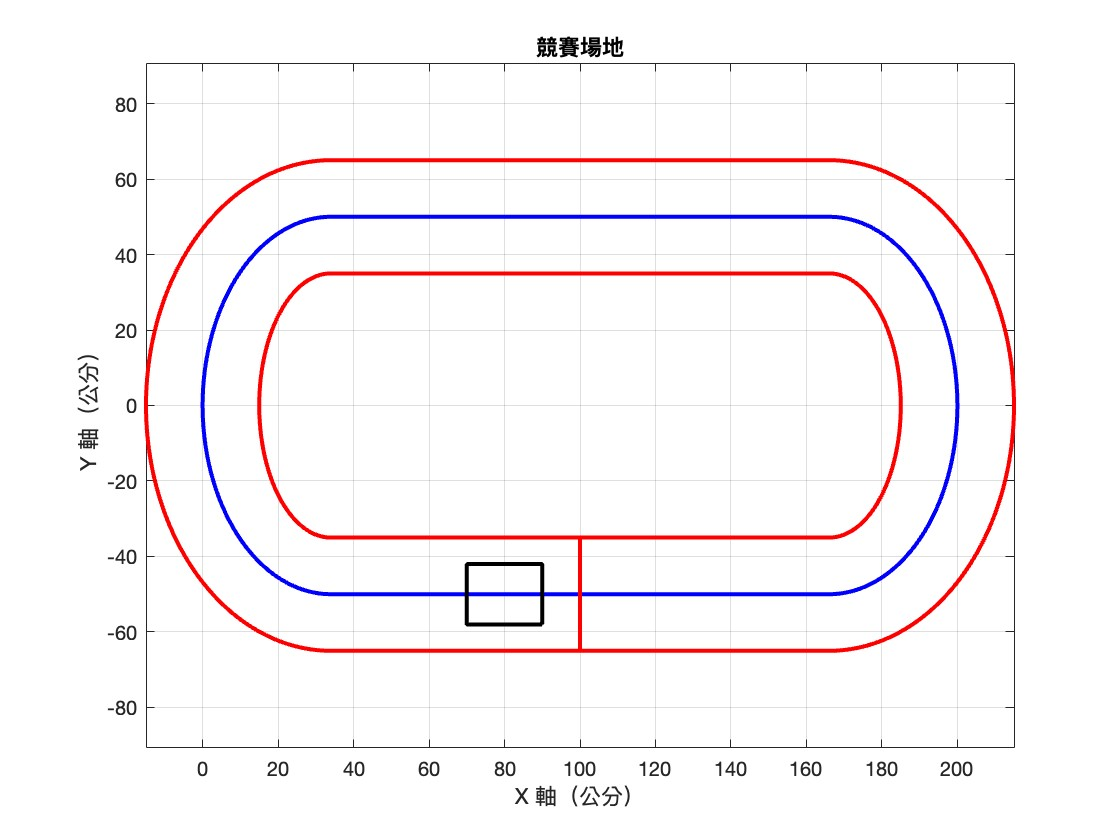
\includegraphics[width=0.8\textwidth]{untitled01.jpg}     %圖片檔案名稱
    \caption{以matlab繪製出競賽場地}    %圖片檔案名稱
    \label{fig:00}    %為圖片添加標籤
    %如\ref{fig:2}所示
\end{figure}

在畫出競賽場地後，依照以下以下幾項前提進行模擬：

\begin{itemize}
    \item 車身長寬為20cm$\times$16cm(目前尚未製作車體，以在機電整合做的車模擬)
    \item 車輛在取得控制命令後立即轉向及移動
    \item 目前在個人電腦測試程式運行時間為0.2秒
    \item 偵測車輛前方5cm、10cm與20cm處如(圖\ref{fig:02}所示)
    \item 旋轉中心為車輛正中心
    \item 車輛在移動過程中無任何干擾
\end{itemize}

\begin{figure}[H]
    \centering
    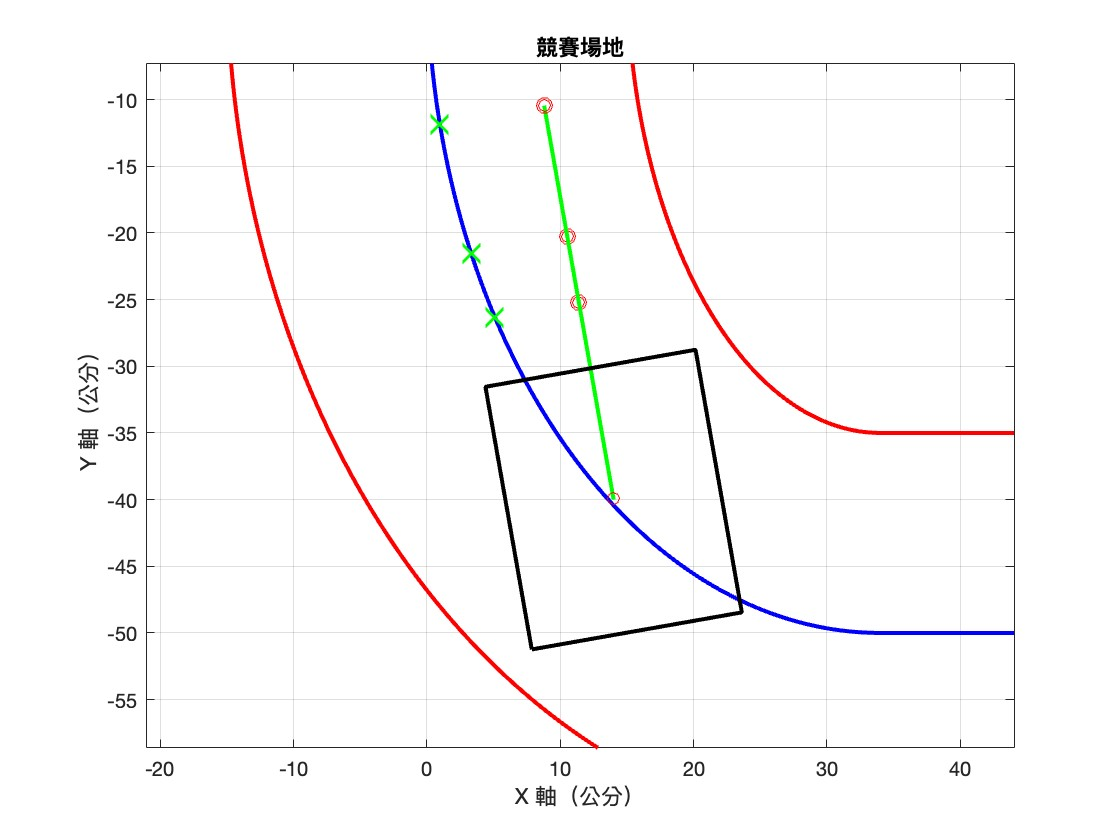
\includegraphics[width=0.8\textwidth]{untitled02.jpg}     %圖片檔案名稱
    \caption{車輛偵測模擬圖}    %圖片檔案名稱
    \label{fig:02}    %為圖片添加標籤
    %如\ref{fig:2}所示
\end{figure}

下圖(圖\ref{fig:02})為依照設計的模糊控制器模擬之結果，車輛出發時，車頭完全對齊標線，無任何距離及角度偏差，車輛每0.2秒執行一次速度更改。

\begin{figure}[H]
    \centering
    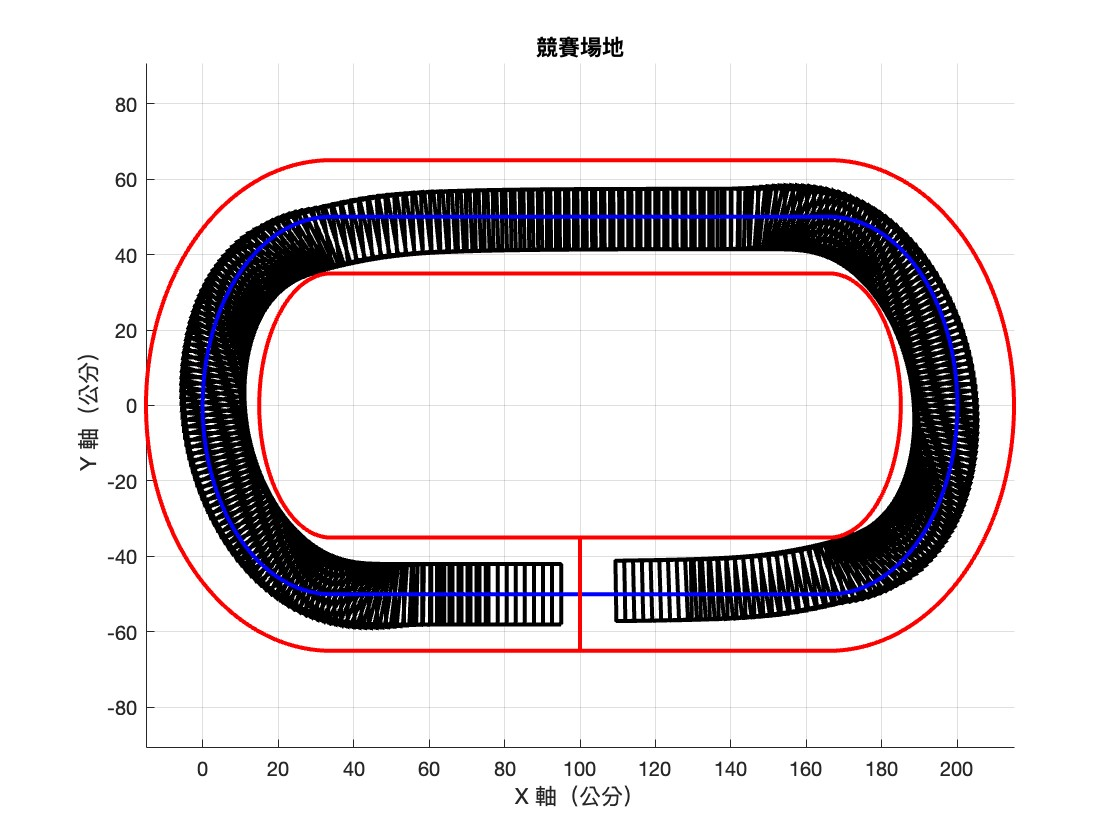
\includegraphics[width=0.8\textwidth]{0_0_02_1.jpg}     %圖片檔案名稱
    \caption{車輛路徑模擬圖}    %圖片檔案名稱
    \label{fig:01}    %為圖片添加標籤
    %如\ref{fig:2}所示
\end{figure}

由上圖(圖\ref{fig:02})可知，目前設計的模糊控制器是可行的，且車輛會在出發54.2秒後抵達終點。圖\ref{fig:0_0_02_2}及圖\ref{fig:0_0_02_4}為車輛對沿途移動速度及角速度。

\begin{figure}[H]
    \centering
    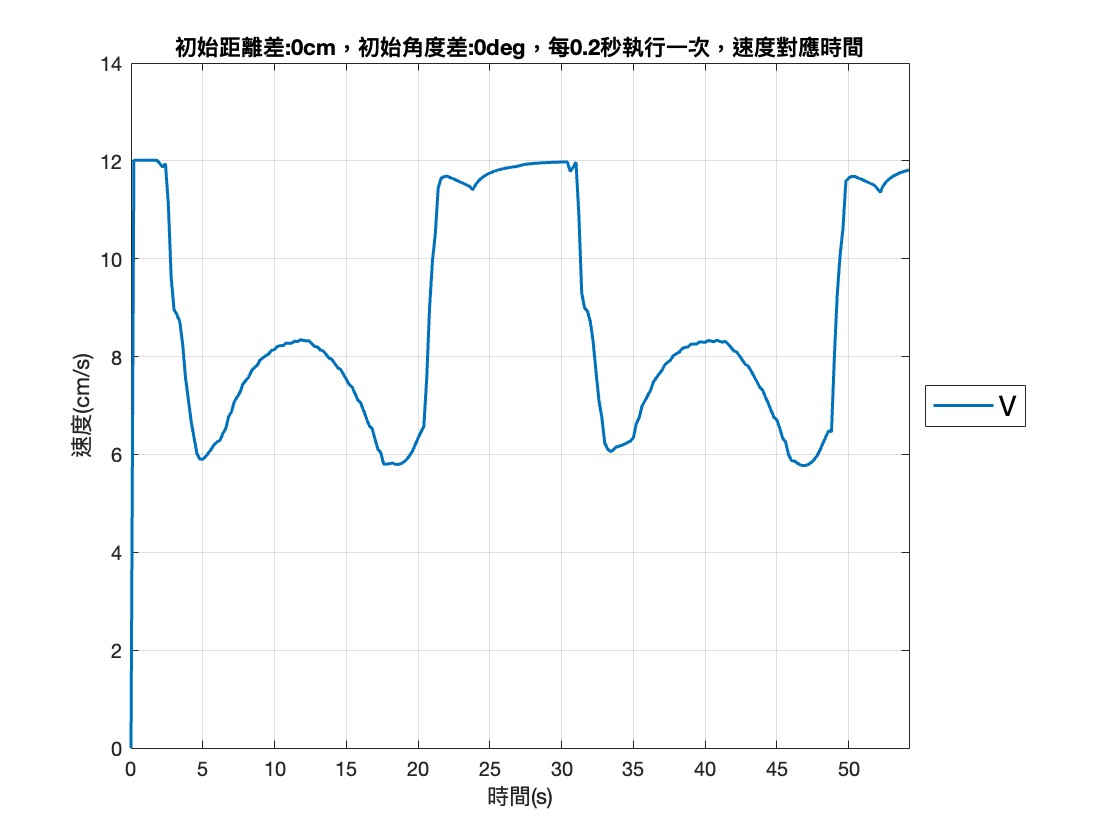
\includegraphics[width=0.8\textwidth]{0_0_02_2.jpg}     %圖片檔案名稱
    \caption{車輛速度對應時間圖}    %圖片檔案名稱
    \label{fig:0_0_02_2}    %為圖片添加標籤
    %如\ref{fig:2}所示
\end{figure}

\begin{figure}[H]
    \centering
    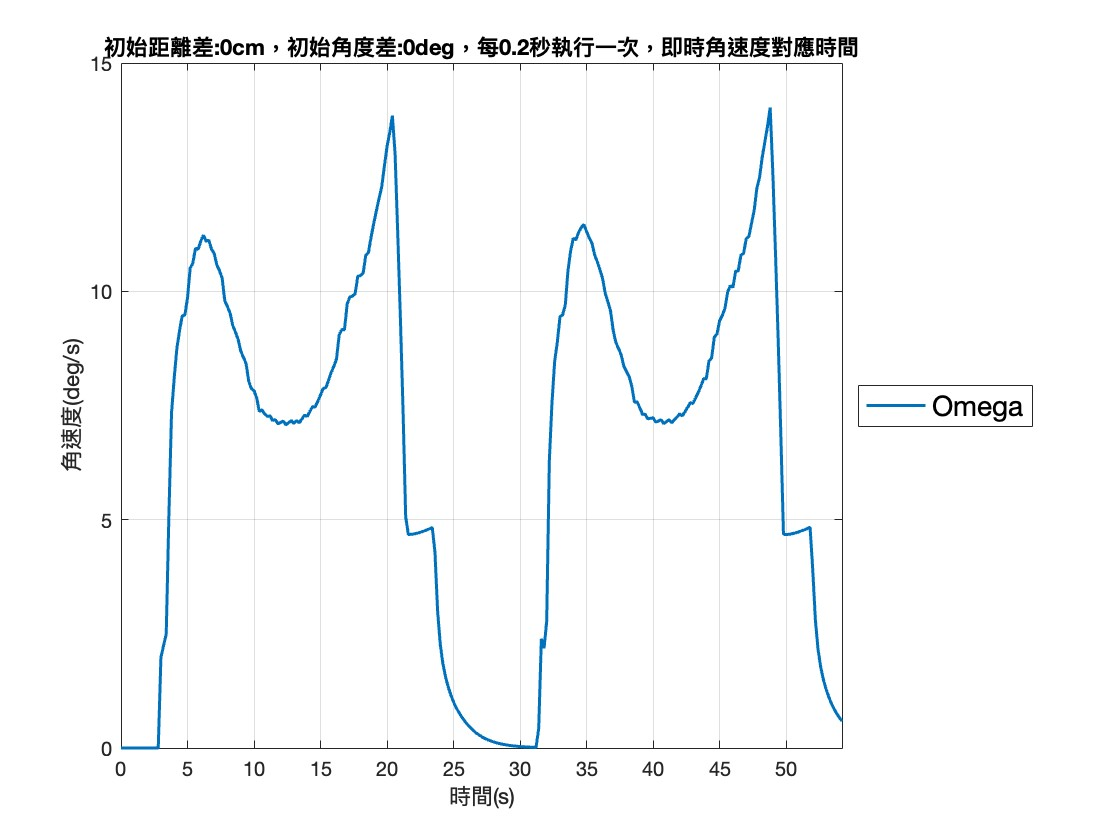
\includegraphics[width=0.8\textwidth]{0_0_02_4.jpg}     %圖片檔案名稱
    \caption{車輛速度對應時間圖}    %圖片檔案名稱
    \label{fig:0_0_02_4}    %為圖片添加標籤
    %如\ref{fig:2}所示
\end{figure}

圖\ref{fig:0_0_02_3}為車輛對沿途移動速度的分量，包含前進速度$V_{x}$及側向速度$V_{y}$。由圖\ref{fig:0_0_02_3}可知因為車輛始終沒有偏離標線太多，
所以側向速度$V_{y}$幾乎為零，正好符合次專題的設計車輛設計。

\begin{figure}[H]
    \centering
    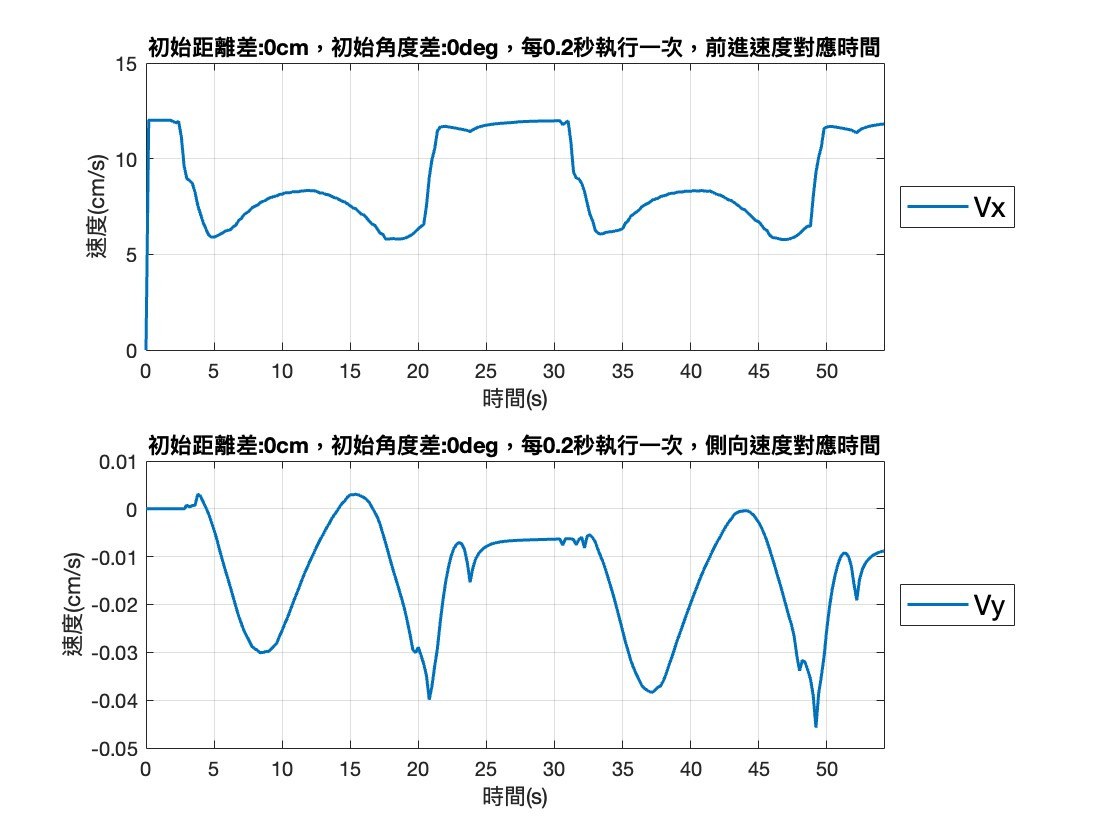
\includegraphics[width=0.8\textwidth]{0_0_02_3.jpg}     %圖片檔案名稱
    \caption{車輛速度分量對應時間圖}    %圖片檔案名稱
    \label{fig:0_0_02_3}    %為圖片添加標籤
    %如\ref{fig:2}所示
\end{figure}

圖\ref{fig:0_0_02_7}及圖\ref{fig:0_0_02_8}為車輛對沿途對標線的偏移量與角度差(以右、順時針為正，以正前方為0度)，由圖(圖\ref{fig:0_0_02_7})可知最大偏移量為6.1$cm$，，由圖(圖\ref{fig:0_0_02_7})可知痾量最大的角度差為17度。
\begin{figure}[H]
    \centering
    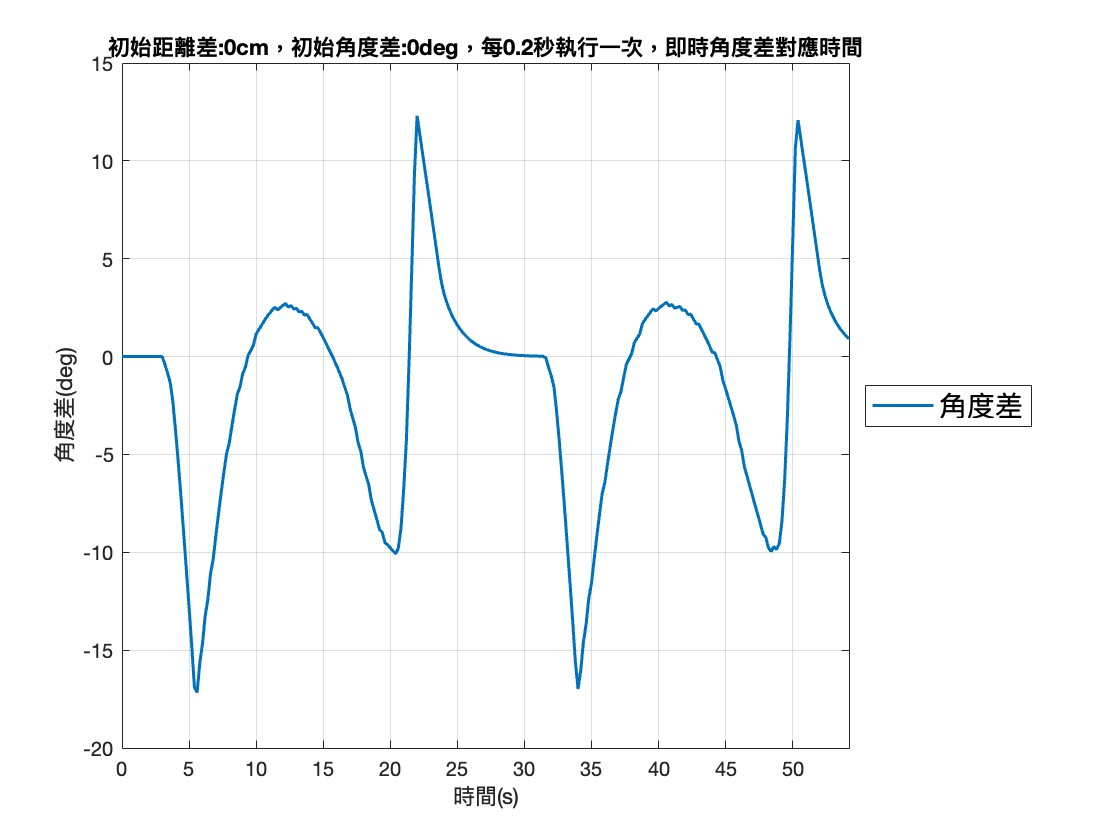
\includegraphics[width=0.8\textwidth]{0_0_02_7.jpg}     %圖片檔案名稱
    \caption{車輛與標線距離差對應時間圖}    %圖片檔案名稱
    \label{fig:0_0_02_7}    %為圖片添加標籤
    %如\ref{fig:2}所示
\end{figure}

\begin{figure}[H]
    \centering
    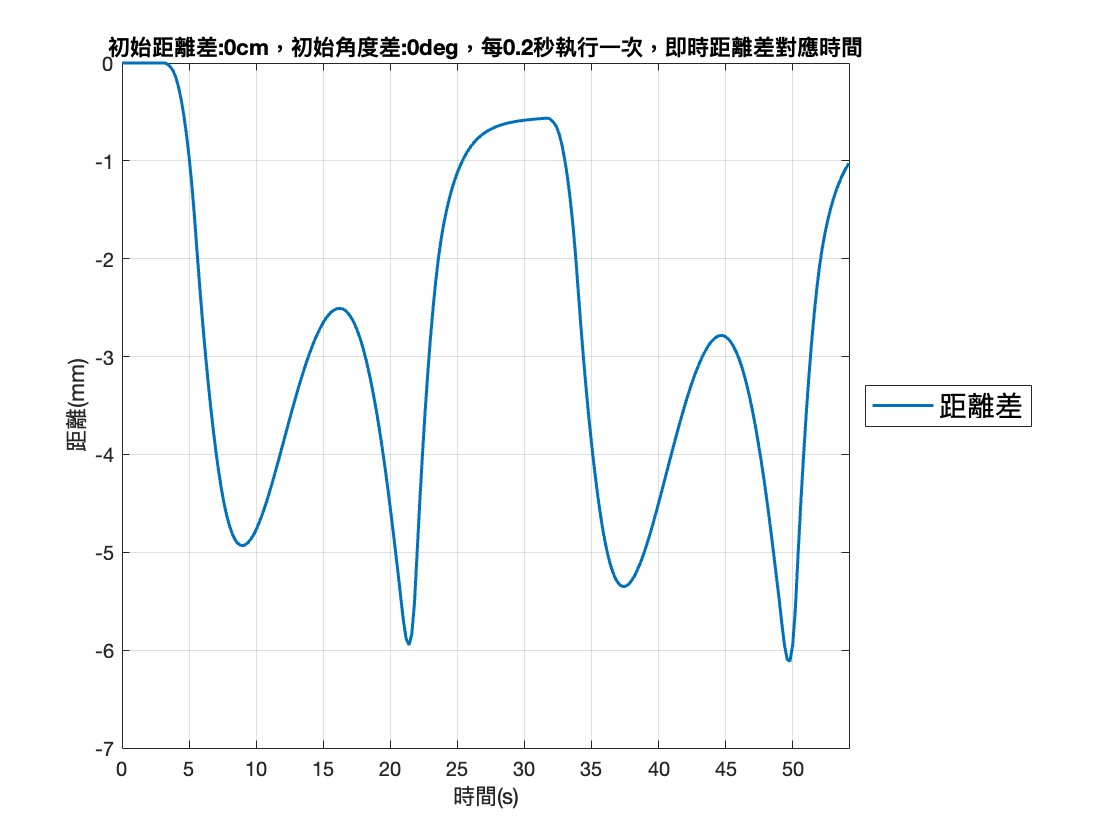
\includegraphics[width=0.8\textwidth]{0_0_02_8.jpg}     %圖片檔案名稱
    \caption{車輛與標線角度差對應時間圖}    %圖片檔案名稱
    \label{fig:0_0_02_8}    %為圖片添加標籤
    %如\ref{fig:2}所示
\end{figure}

圖\ref{fig:0_0_02_5}及圖\ref{fig:0_0_02_6}為車輛對沿途偵測到標線的偏移量與角度差(以右、順時針為正，以正前方為0度)。

\begin{figure}[H]
    \centering
    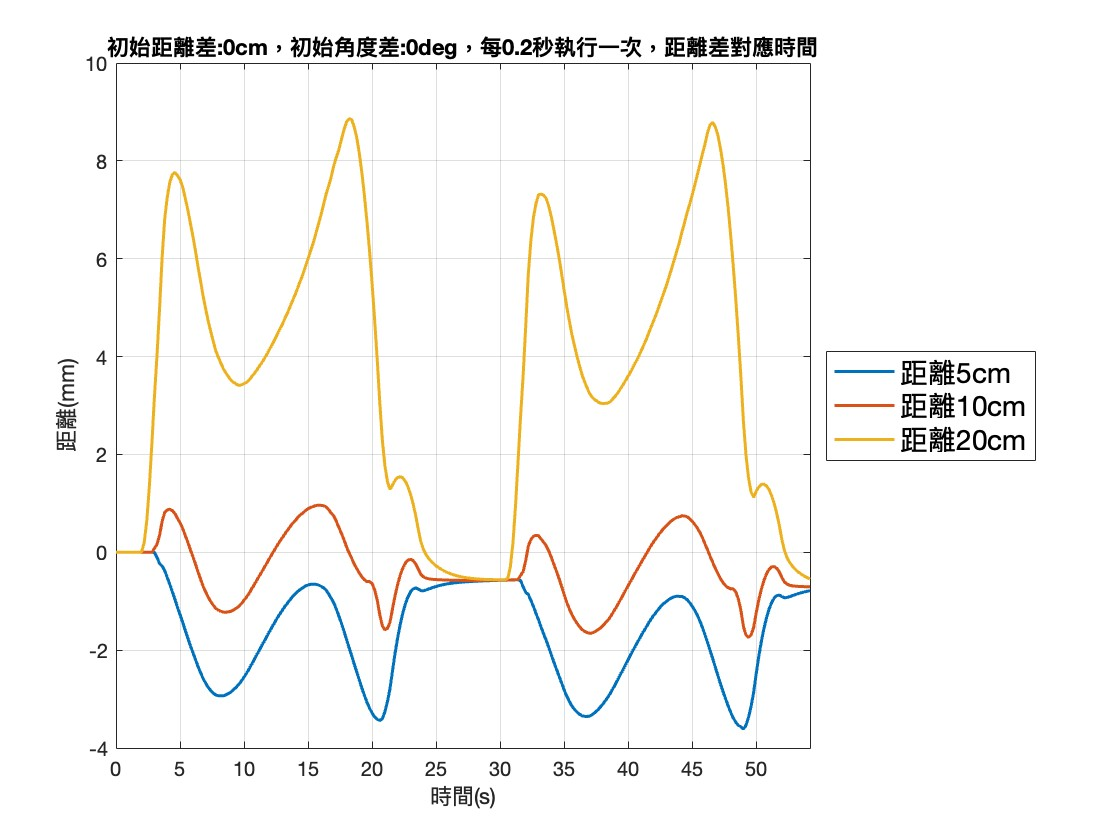
\includegraphics[width=0.8\textwidth]{0_0_02_5.jpg}     %圖片檔案名稱
    \caption{車輛偵測標線距離差對應時間圖}    %圖片檔案名稱
    \label{fig:0_0_02_5}    %為圖片添加標籤
    %如\ref{fig:2}所示
\end{figure}

\begin{figure}[H]
    \centering
    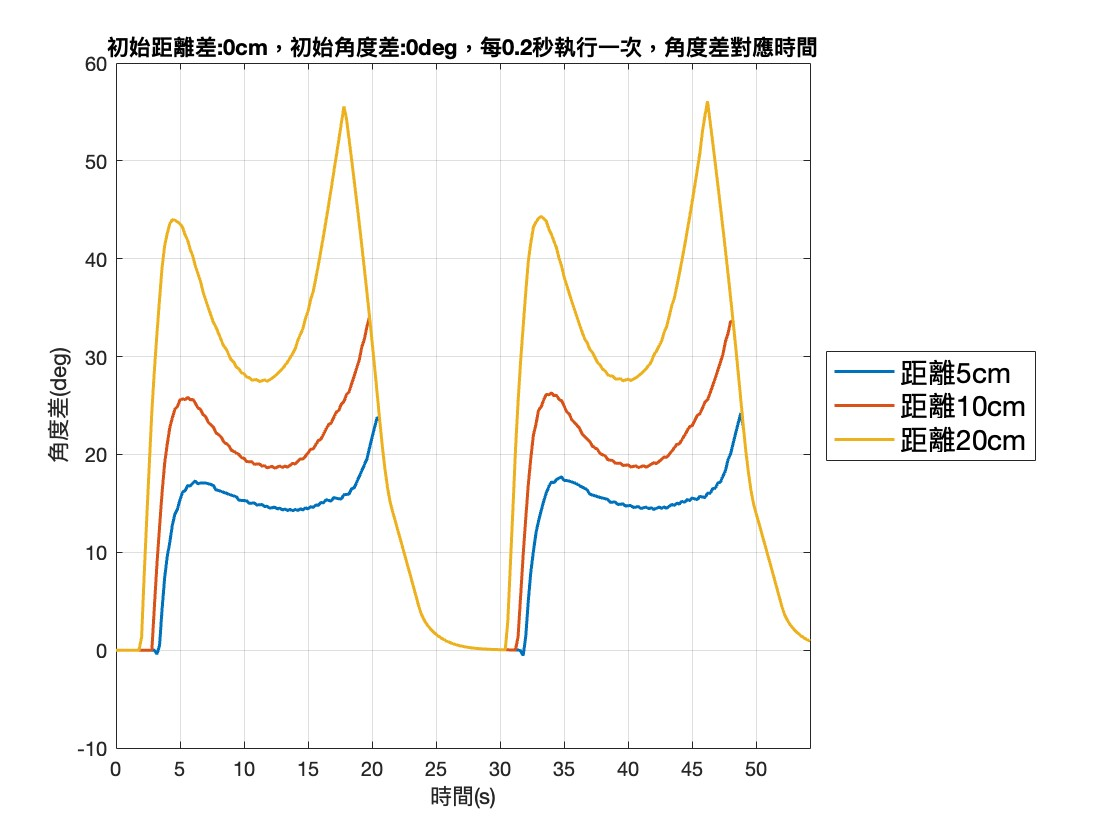
\includegraphics[width=0.8\textwidth]{0_0_02_6.jpg}     %圖片檔案名稱
    \caption{車輛偵測標線角度差對應時間圖}    %圖片檔案名稱
    \label{fig:0_0_02_6}    %為圖片添加標籤
    %如\ref{fig:2}所示
\end{figure}

由以上分析可知此控制系統是可以達成任務的。接下來是分析此控制系統之穩健性。分析內容包含影像的接收頻率(控制命令間隔)，與出發時車輛放置位置與角度。

考慮到影像接收可能不穩定或樹莓派運算時間較長，首先分析控制命令間隔的容許度。由圖\ref{fig:0_0_1_1}可知每1秒進行一次控制是可行的。
而由圖\ref{fig:0_0_2_1}可知，若以每2秒進行一次控制，將會在過彎時會稍微超出界線。

\begin{figure}[H]
    \centering
    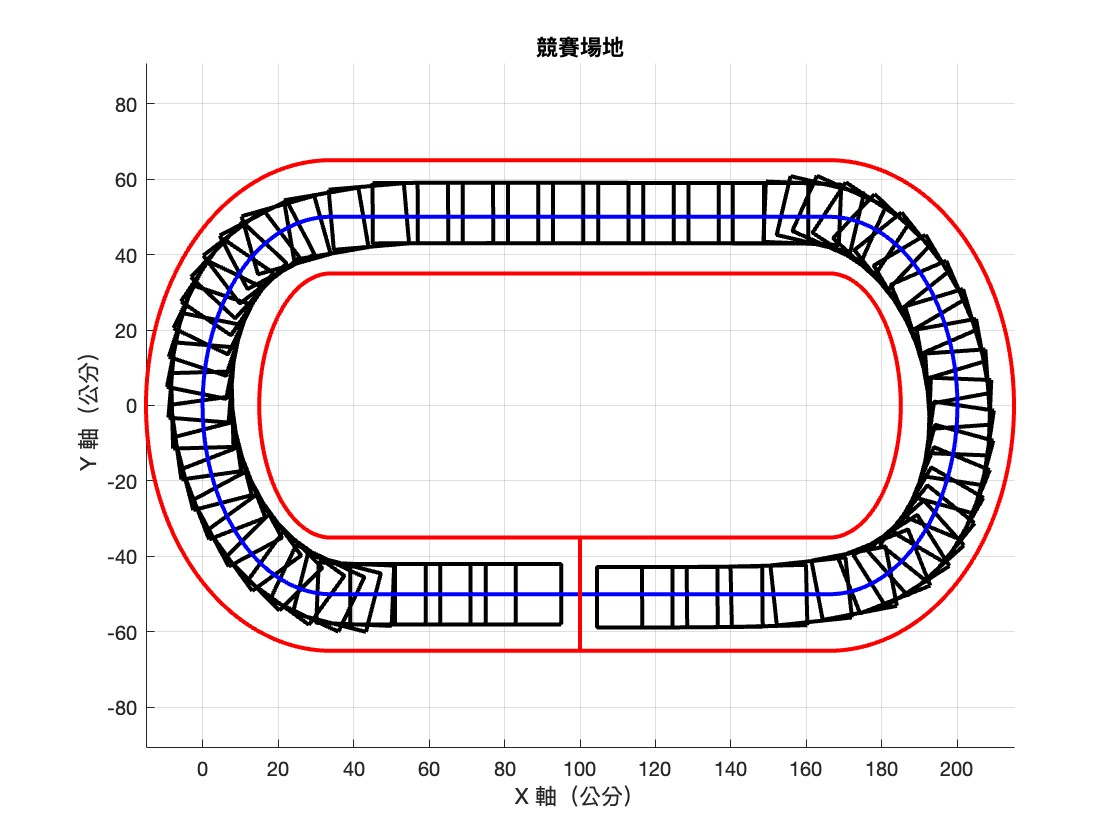
\includegraphics[width=0.8\textwidth]{0_0_1_1.jpg}     %圖片檔案名稱
    \caption{每1秒控制一次之車輛移動路徑模擬圖}    %圖片檔案名稱
    \label{fig:0_0_1_1}    %為圖片添加標籤
    %如\ref{fig:0_0_1_1}所示
\end{figure}

\begin{figure}[H]
    \centering
    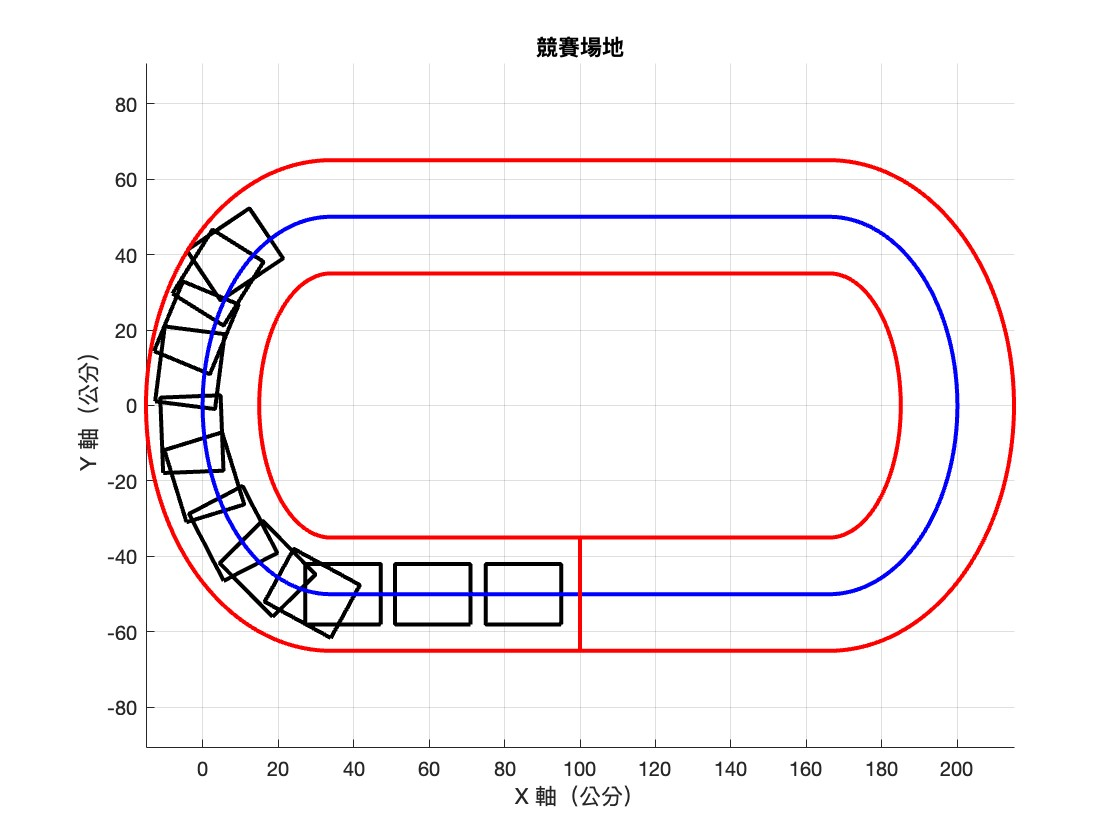
\includegraphics[width=0.8\textwidth]{0_0_2_1.jpg}     %圖片檔案名稱
    \caption{每2秒控制一次之車輛移動路徑模擬圖}    %圖片檔案名稱
    \label{fig:0_0_2_1}    %為圖片添加標籤
    %如\ref{fig:2}所示
\end{figure}

模擬出此模糊控制器最長的控制時間間隔為1.67秒，若超過1.67秒(圖\ref{fig:0_0_17_1})，便會碰到界線。

\begin{figure}[H]
    \centering
    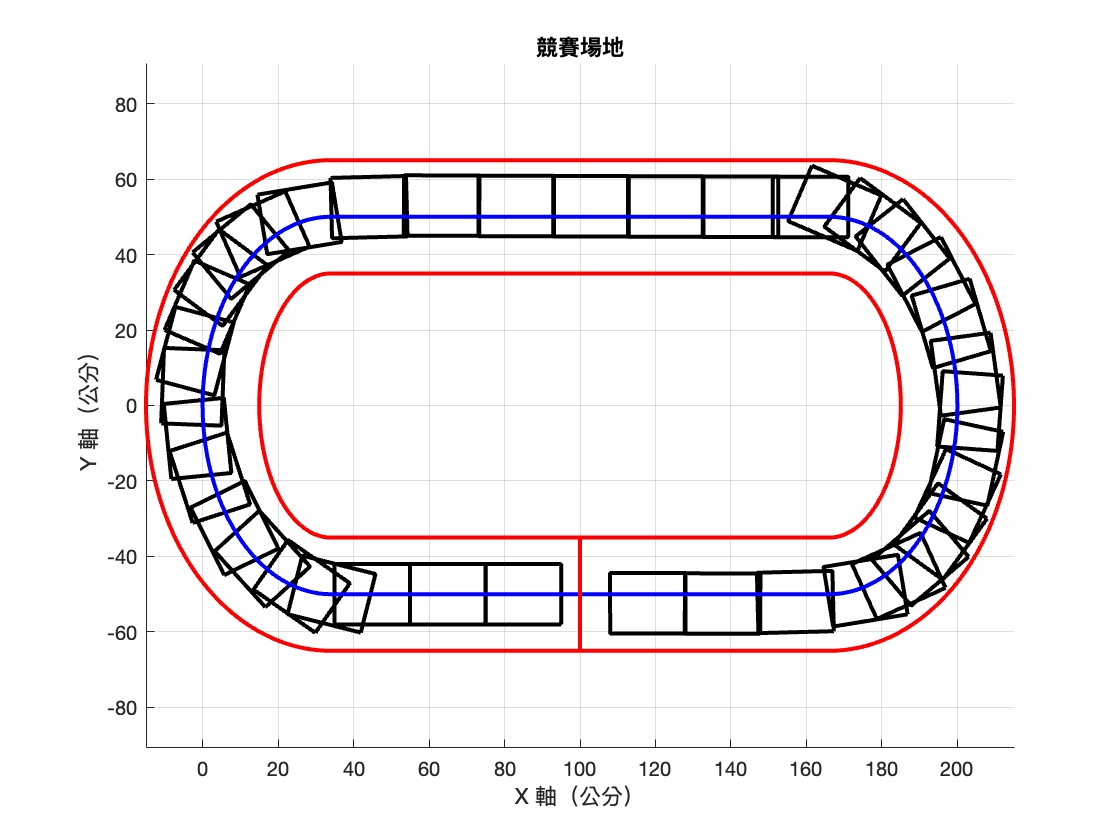
\includegraphics[width=0.8\textwidth]{0_0_17_1.jpg}     %圖片檔案名稱
    \caption{每1.7秒控制一次之車輛移動路徑模擬圖}    %圖片檔案名稱
    \label{fig:0_0_17_1}    %為圖片添加標籤
    %如\ref{fig:2}所示
\end{figure}

接下來是模擬車輛在開始時的位置與角度偏移，以下模擬均以每0.2秒運算一次進行模擬。
模擬初始角度有15度到-55度的偏差。如圖\ref{fig:0_15_02_1}～圖\ref{fig:0_-55_02_1}所示。
可知在15度(圖\ref{fig:0_15_02_1})、在-55度圖\ref{fig:0_-55_02_1}之外會出界，在10度(圖\ref{fig:0_10_02_1})到-50度(圖\ref{fig:0_-50_02_1})間是可以到達終點的。

\begin{figure}[H]
    \centering
    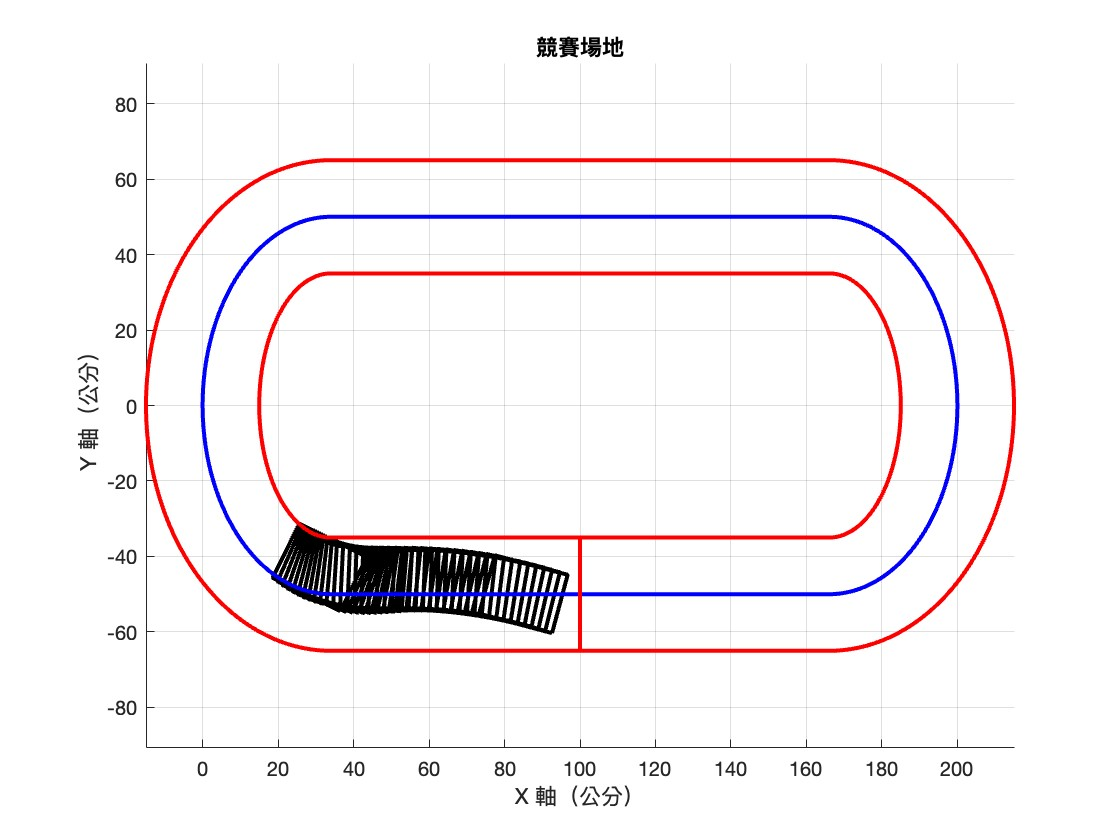
\includegraphics[width=0.8\textwidth]{0_15_02_1.jpg}     %圖片檔案名稱
    \caption{初始角度為15度之車輛移動路徑模擬圖}    %圖片檔案名稱
    \label{fig:0_15_02_1}    %為圖片添加標籤
    %如\ref{fig:2}所示
\end{figure}

\begin{figure}[H]
    \centering
    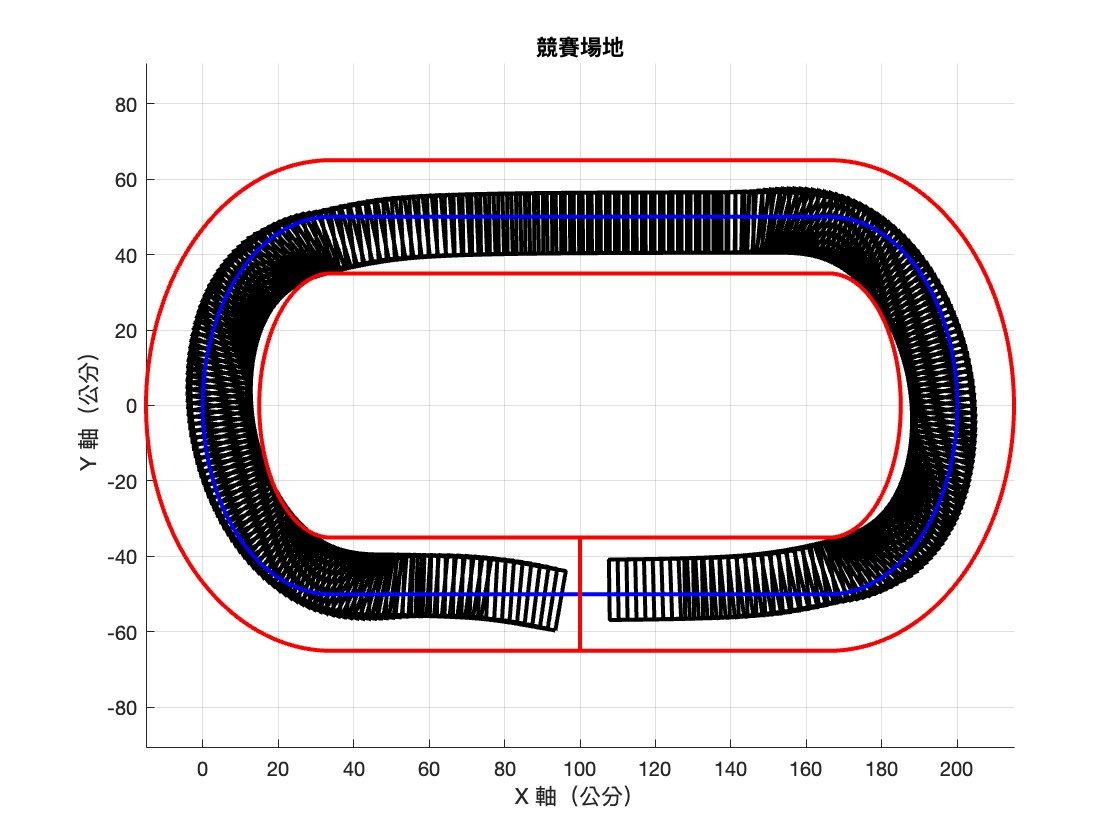
\includegraphics[width=0.8\textwidth]{0_10_02_1.jpg}     %圖片檔案名稱
    \caption{初始角度為10度之車輛移動路徑模擬圖}    %圖片檔案名稱
    \label{fig:0_10_02_1}    %為圖片添加標籤
    %如\ref{fig:2}所示
\end{figure}

\begin{figure}[H]
    \centering
    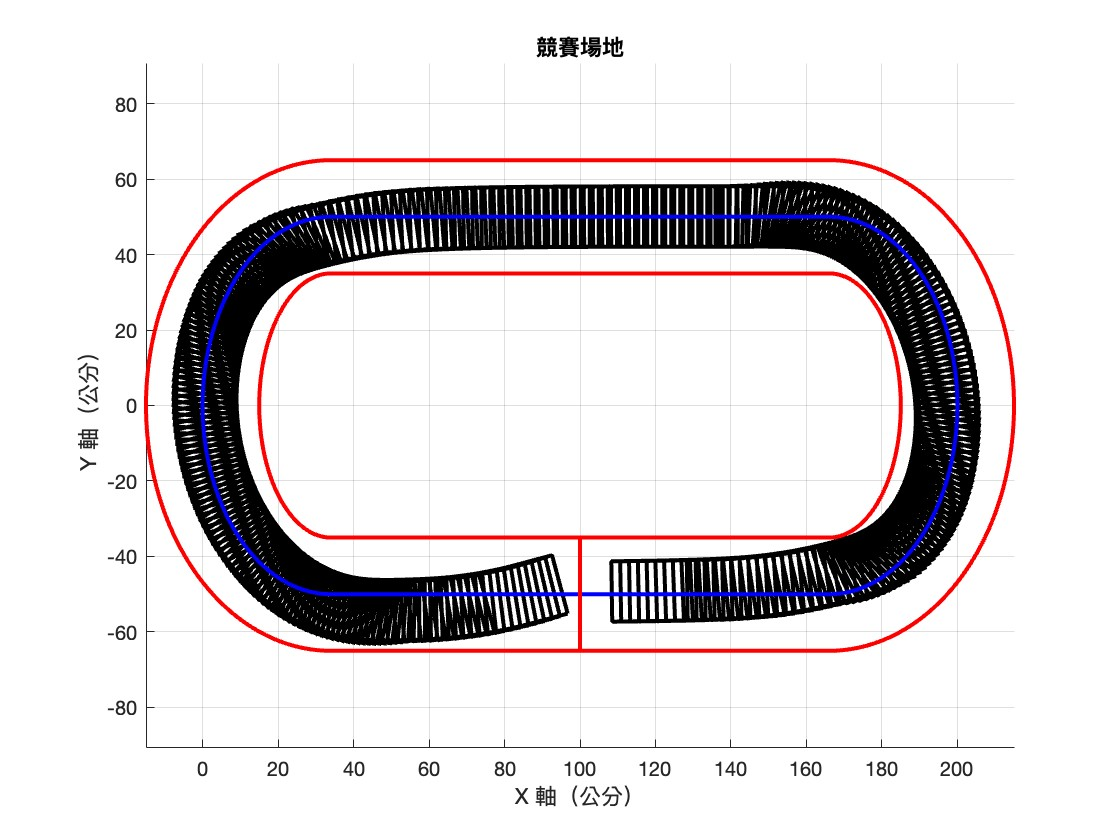
\includegraphics[width=0.8\textwidth]{0_-15_02_1.jpg}     %圖片檔案名稱
    \caption{初始角度為-15度之車輛移動路徑模擬圖}    %圖片檔案名稱
    %如\ref{fig:2}所示
\end{figure}

\begin{figure}[H]
    \centering
    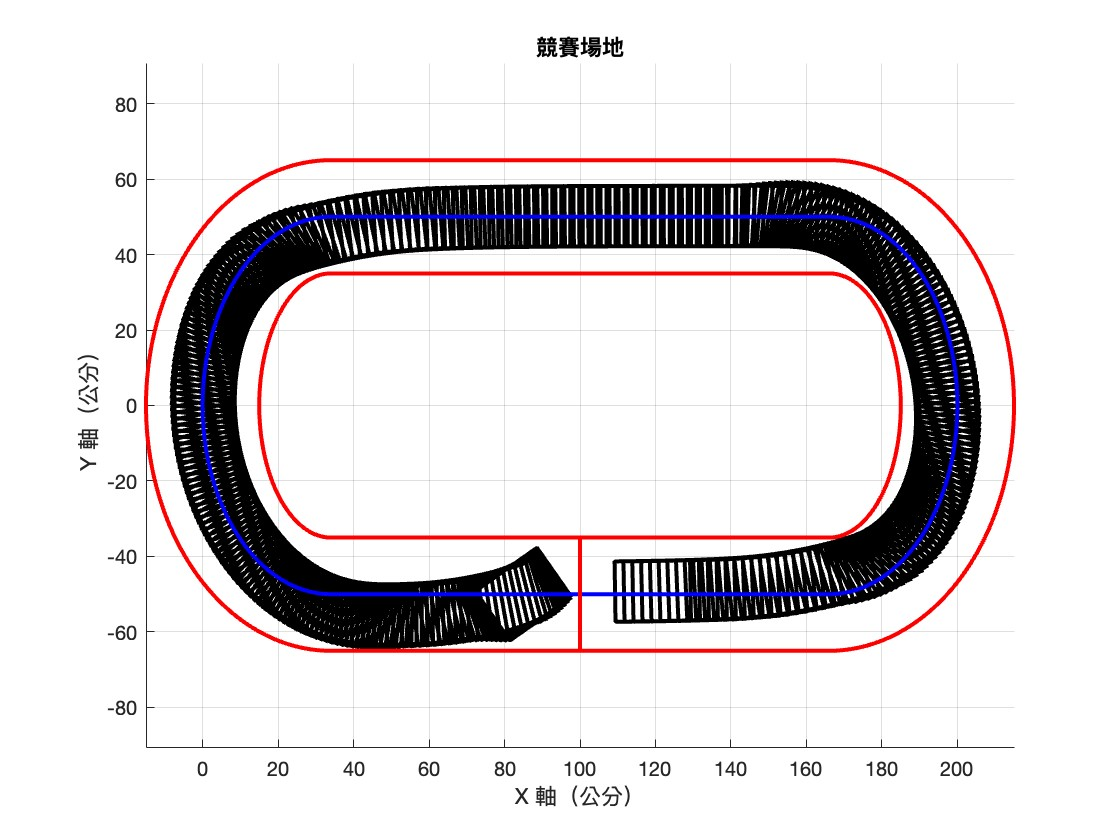
\includegraphics[width=0.8\textwidth]{0_-35_02_1.jpg}     %圖片檔案名稱
    \caption{初始角度為-35度之車輛移動路徑模擬圖}    %圖片檔案名稱
    %如\ref{fig:2}所示
\end{figure}

\begin{figure}[H]
    \centering
    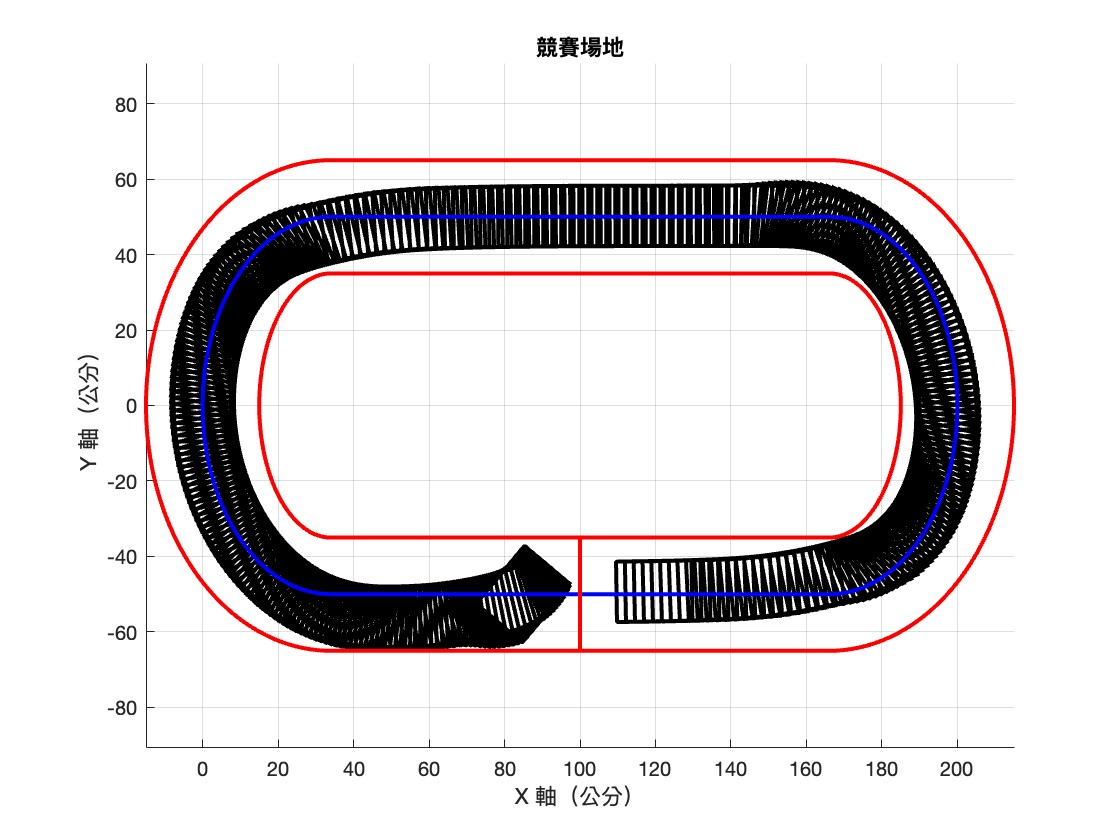
\includegraphics[width=0.8\textwidth]{0_-50_02_1.jpg}     %圖片檔案名稱
    \caption{初始角度為-50度之車輛移動路徑模擬圖}    %圖片檔案名稱
    \label{fig:0_-50_02_1}    %為圖片添加標籤
    %如\ref{fig:2}所示
\end{figure}

\begin{figure}[H]
    \centering
    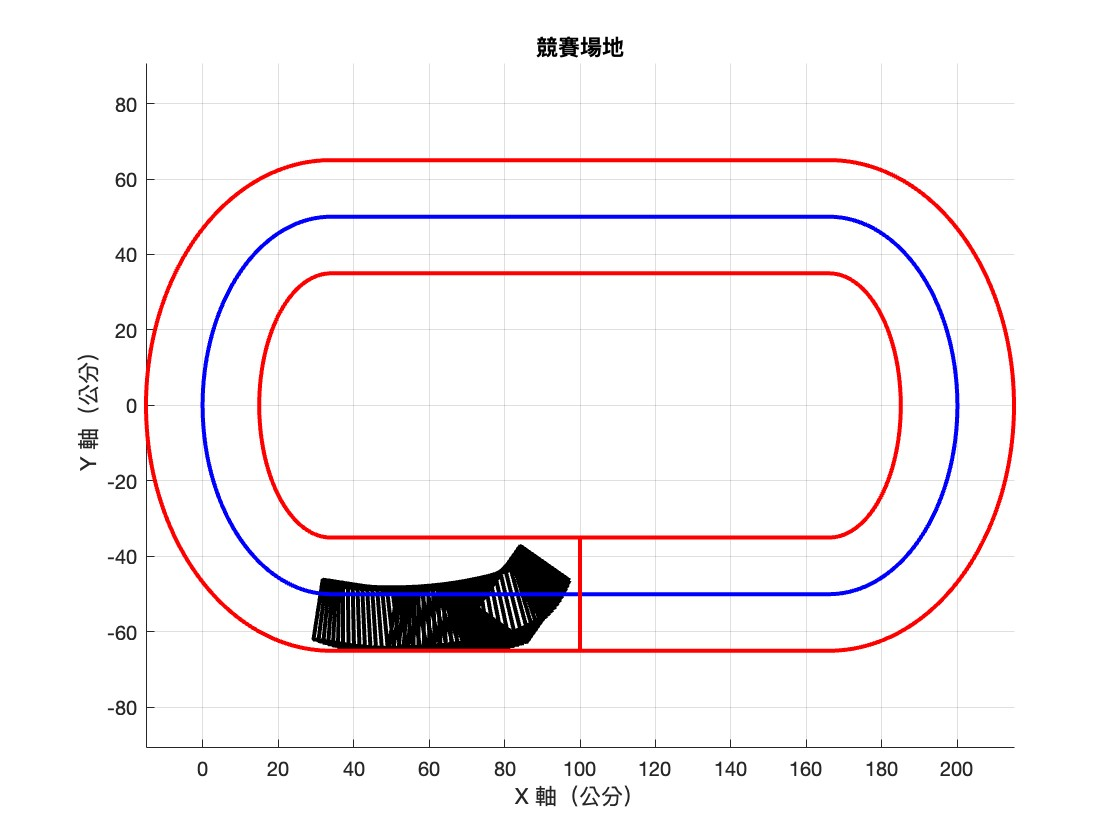
\includegraphics[width=0.8\textwidth]{0_-55_02_1.jpg}     %圖片檔案名稱
    \caption{初始角度為-55度之車輛移動路徑模擬圖}    %圖片檔案名稱
    \label{fig:0_-55_02_1}    %為圖片添加標籤
    %如\ref{fig:2}所示
\end{figure}

最後模擬初始偏差有15$cm$到-55$cm$。如圖\ref{fig:4_0_02_1}～圖\ref{fig:07_0_02_1}所示。
可知在4$cm$(圖\ref{fig:4_0_02_1})、在4$cm$圖\ref{fig:07_0_02_1}之外會出界，
在3.5$cm$(圖\ref{fig:35_0_02_1})到4$cm$度(圖\ref{fig:065_0_02_1})間是可以到達終點的。
\begin{figure}[H]
    \centering
    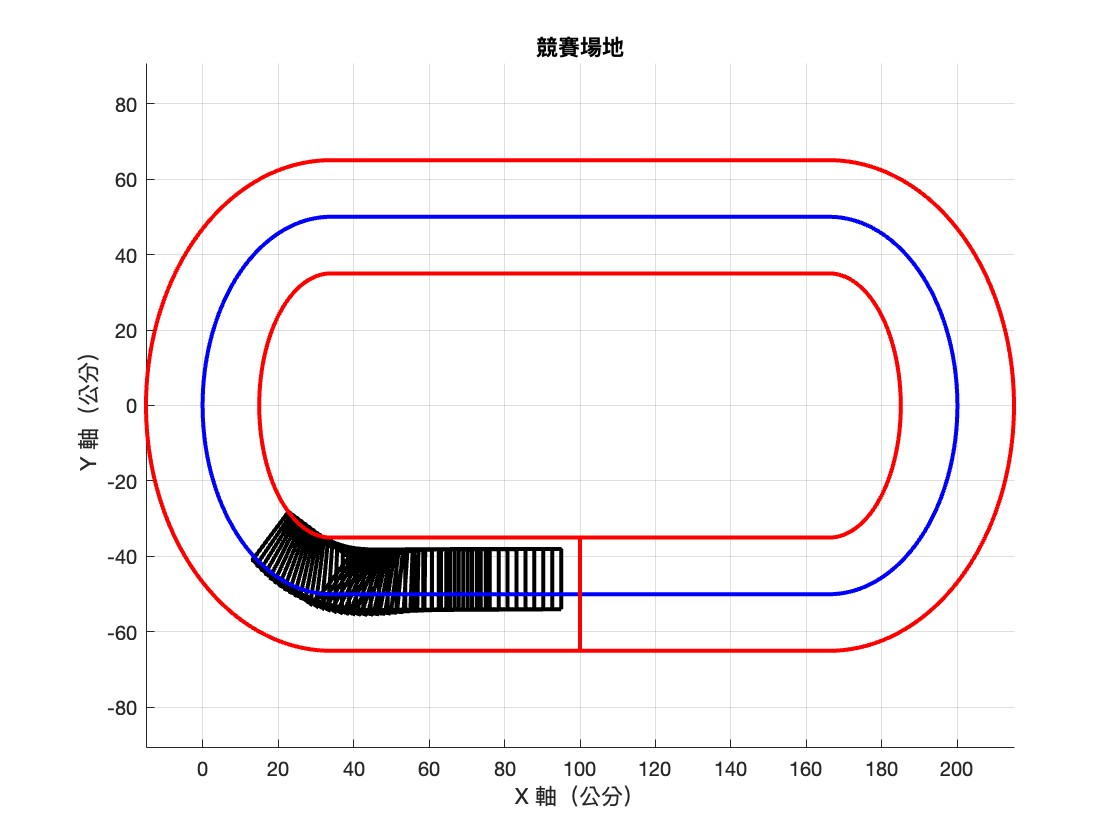
\includegraphics[width=0.8\textwidth]{4_0_02_1.jpg}     %圖片檔案名稱
    \caption{初始偏差為4$cm$之車輛移動路徑模擬圖}    %圖片檔案名稱
    \label{fig:4_0_02_1}    %為圖片添加標籤
    %如\ref{fig:2}所示
\end{figure}

\begin{figure}[H]
    \centering
    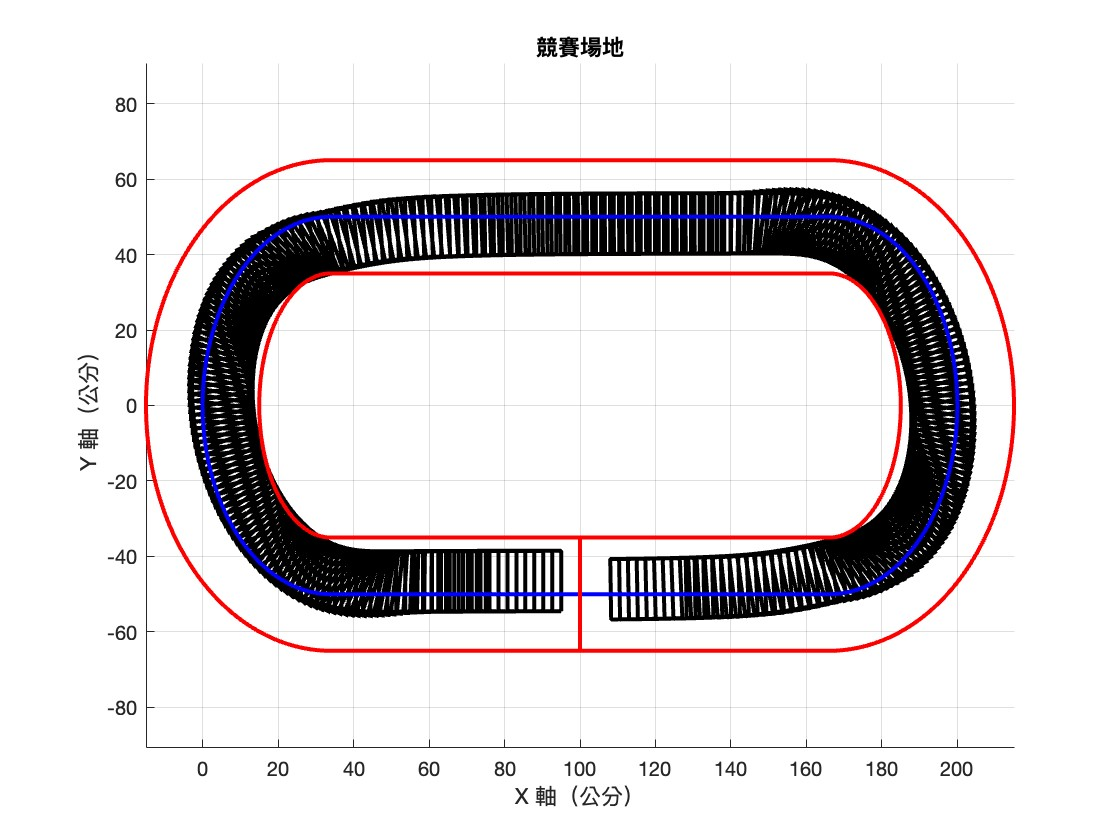
\includegraphics[width=0.8\textwidth]{35_0_02_1.jpg}     %圖片檔案名稱
    \caption{初始偏差為3.5$cm$之車輛移動路徑模擬圖}    %圖片檔案名稱
    \label{fig:35_0_02_1}    %為圖片添加標籤
    %如\ref{fig:2}所示
\end{figure}

\begin{figure}[H]
    \centering
    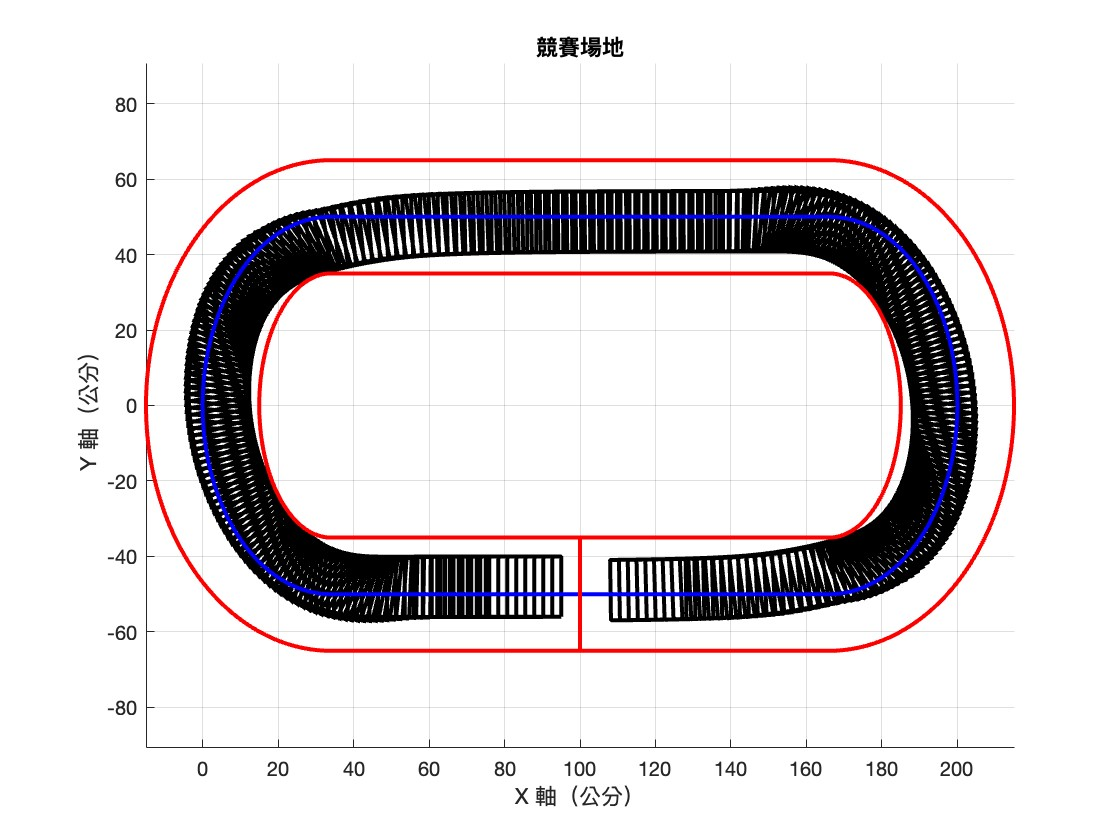
\includegraphics[width=0.8\textwidth]{2_0_02_1.jpg}     %圖片檔案名稱
    \caption{初始偏差為2$cm$之車輛移動路徑模擬圖}    %圖片檔案名稱
    %如\ref{fig:2}所示
\end{figure}

\begin{figure}[H]
    \centering
    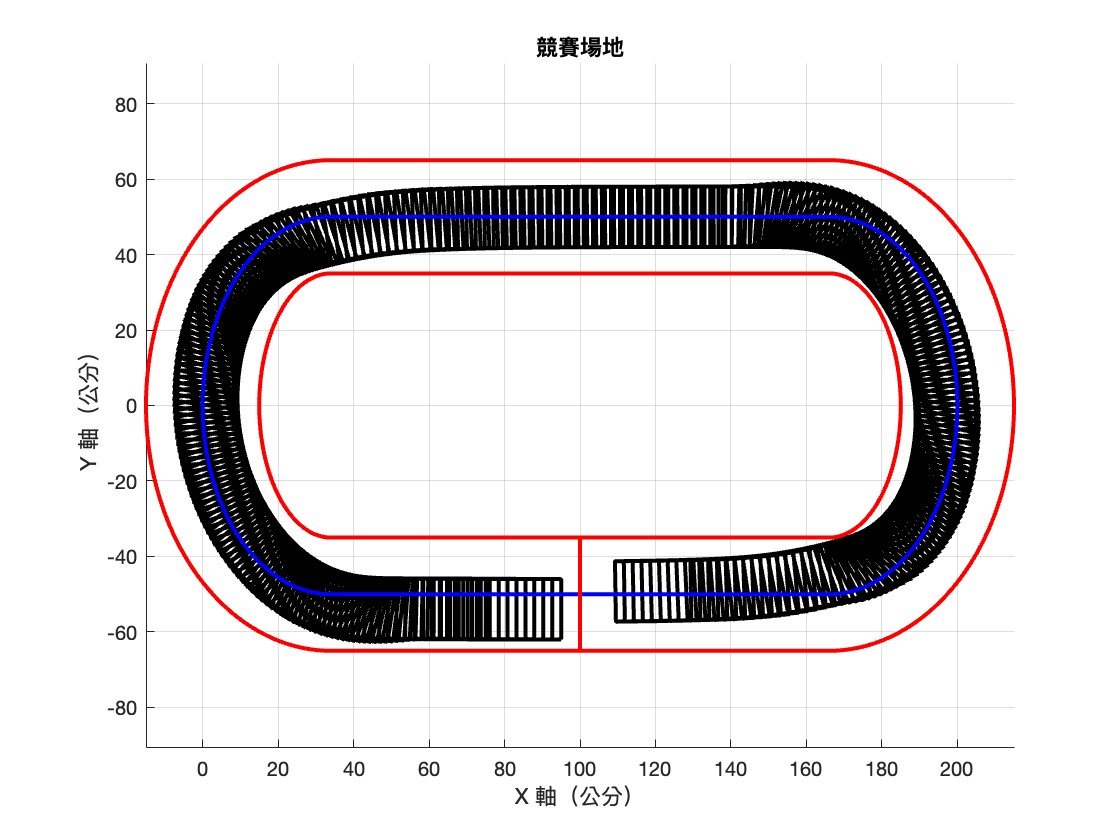
\includegraphics[width=0.8\textwidth]{04_0_02_1.jpg}     %圖片檔案名稱
    \caption{初始偏差為-4$cm$之車輛移動路徑模擬圖}    %圖片檔案名稱
    %如\ref{fig:2}所示
\end{figure}

\begin{figure}[H]
    \centering
    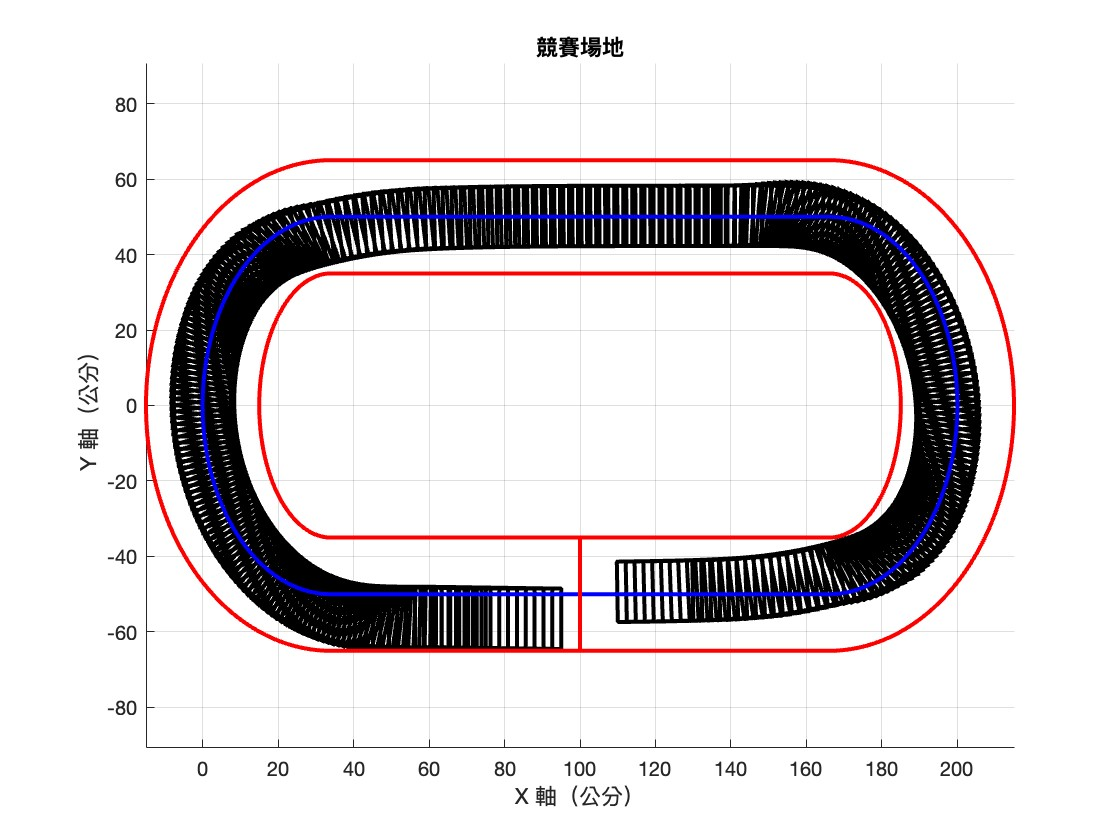
\includegraphics[width=0.8\textwidth]{065_0_02_1.jpg}     %圖片檔案名稱
    \caption{初始偏差為-6.5$cm$之車輛移動路徑模擬圖}    %圖片檔案名稱
    \label{fig:065_0_02_1}    %為圖片添加標籤
    %如\ref{fig:2}所示
\end{figure}

\begin{figure}[H]
    \centering
    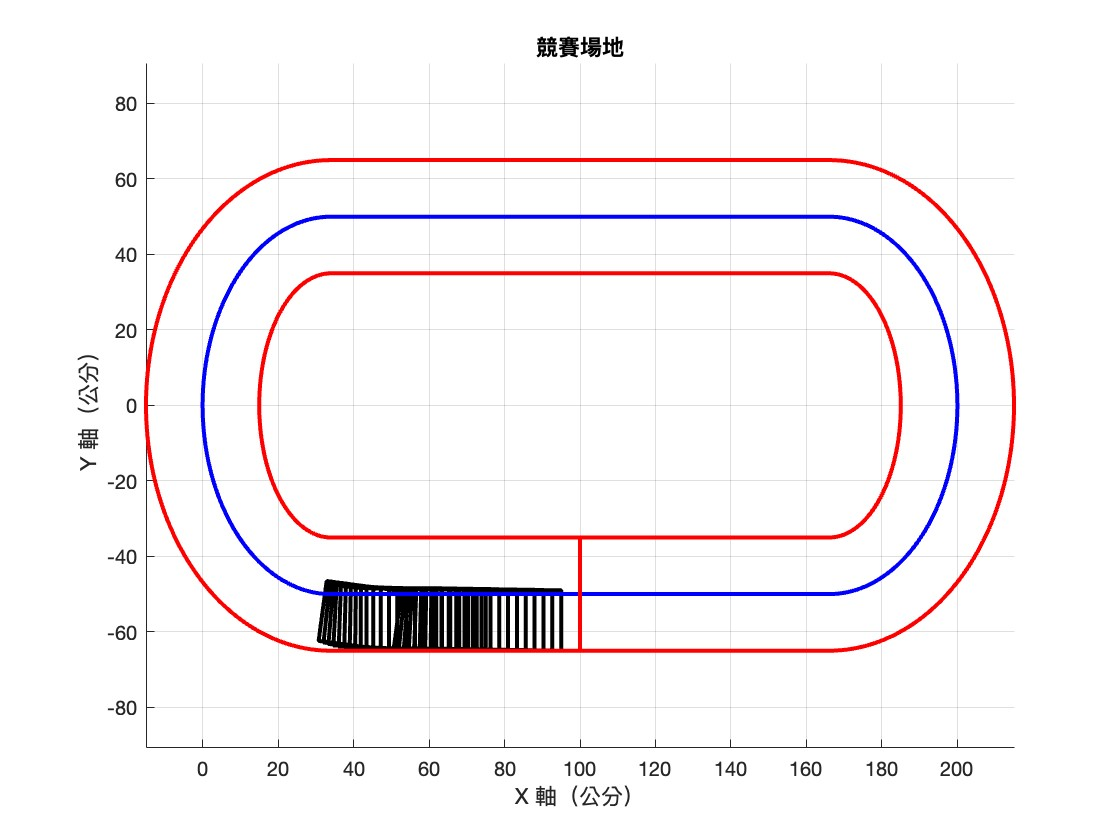
\includegraphics[width=0.8\textwidth]{07_0_02_1.jpg}     %圖片檔案名稱
    \caption{初始偏差為-7$cm$之車輛移動路徑模擬圖}    %圖片檔案名稱
    \label{fig:07_0_02_1}    %為圖片添加標籤
    %如\ref{fig:2}所示
\end{figure}

%==============================內文==============================

\subsection{車輛結構優化分析} 
%==============================內文==============================
\hspace{2em}這部分是在做模型的形狀優化，我使用Fusion360來進行分析。
輪椅的大輪的部分預測其會承受20$N$的力，為了方便計算，我先畫120$\circ$的扇形，輪胎外
徑為140$mm$，內徑為5$mm$，厚度為 5$mm$，使用材料為PLA(材料特性如表\ref{tab:pla}所示)，經過軟體計算，在安全係數還有15的情況下，可以減少59.39$\%$的材料。

\begin{table}[H]
    \centering
    \caption{PLA材料特性}
    \vspace{6pt} % 增加空格
    \label{tab:pla}
    \begin{tabular}{ll}
        \toprule
        \textbf{項目} & \textbf{} \\
        \midrule
        密度  & $1.140E-06 (kg/mm^3)$ \\
        楊氏模量  & $2.10(GPa)$ \\
        泊松比  & $0.36$ \\
        屈服祥度  & $26.94(MPa)$ \\
        極限拉伸強度  & $2.1(MPa)$ \\
        導熱率  & $1.6E-04 (W/mm\cdot C)$ \\
        膨脹係數  & $8.57E-05 (1/C)$ \\
        比熱  & $1800 (J/kg\cdot C)$ \\
        \bottomrule
    \end{tabular}
    %如\ref{tab:TT2}所示
\end{table}

接下來再將整個輪框畫出來，再跑一次靜態應力分析，在軸承孔受力 20$N$
的情況下，最大應力為 0.692$MPa$，最小應力為 $1.905\time10^{-4} MPa$。優化結果如表\ref{tab:bf}、圖\ref{fig:45}、圖\ref{fig:46}所示。

\begin{table}[H]
    \centering
    \caption{PLA材料特性}
    \vspace{6pt} % 增加空格
    \label{tab:bf}
    \begin{tabular}{llll}
        \toprule
        \textbf{原始模型} & \textbf{優化後模型}& \textbf{增加比例$\%$} \\
        \midrule
        最大應力($MPa$)         & $0.537$           & $0.692$       &$28.8$\\
        應變                   & $4.329E-06$        & $5.371E-06$   &$24.07$\\
        位移($mm$)              & $2.074E-05$       & $1.466E-05$   &  \\
        質量比($\%$)            & $100$             & $40.61$       & $-59.39$ \\
        \bottomrule
    \end{tabular}
    %如\ref{tab:TT2}所示
\end{table}

\begin{figure}[H]
    \centering
    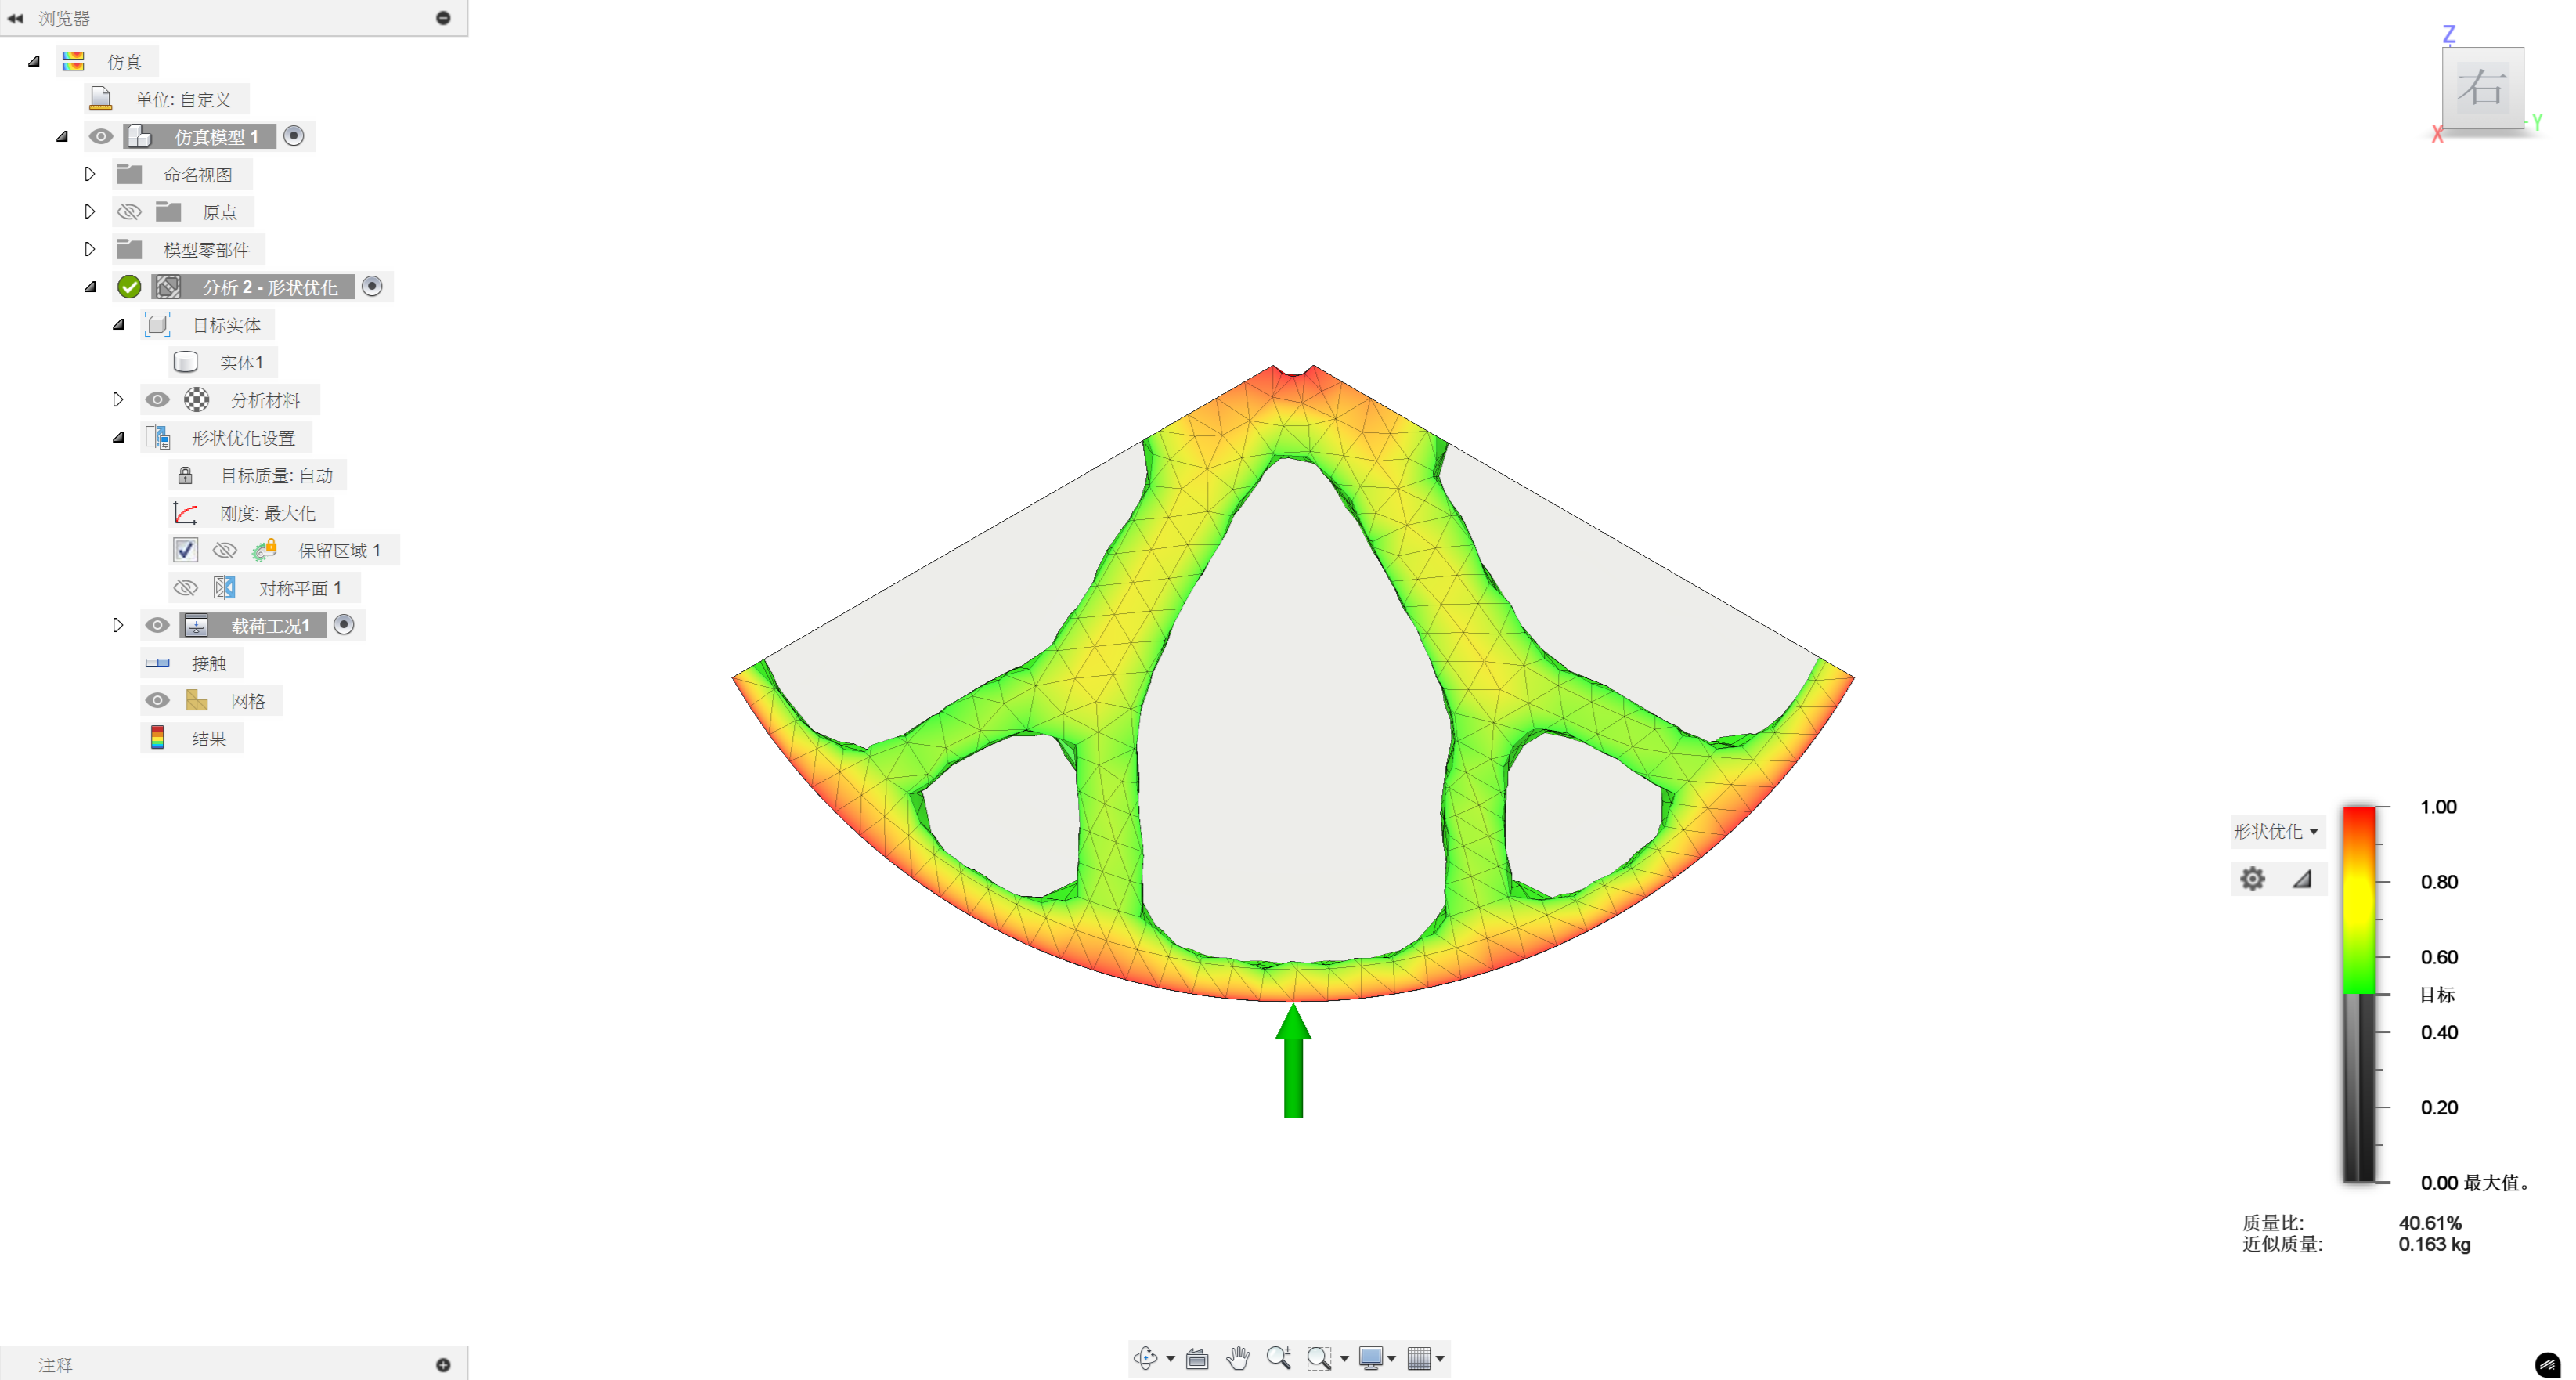
\includegraphics[width=0.7\textwidth]{45.jpg}     %圖片檔案名稱
    \caption{輪椅大輪的形狀優化1}    %圖片檔案名稱
    \label{fig:45}
    %如\ref{fig:example1}所示
\end{figure}

\begin{figure}[H]
    \centering
    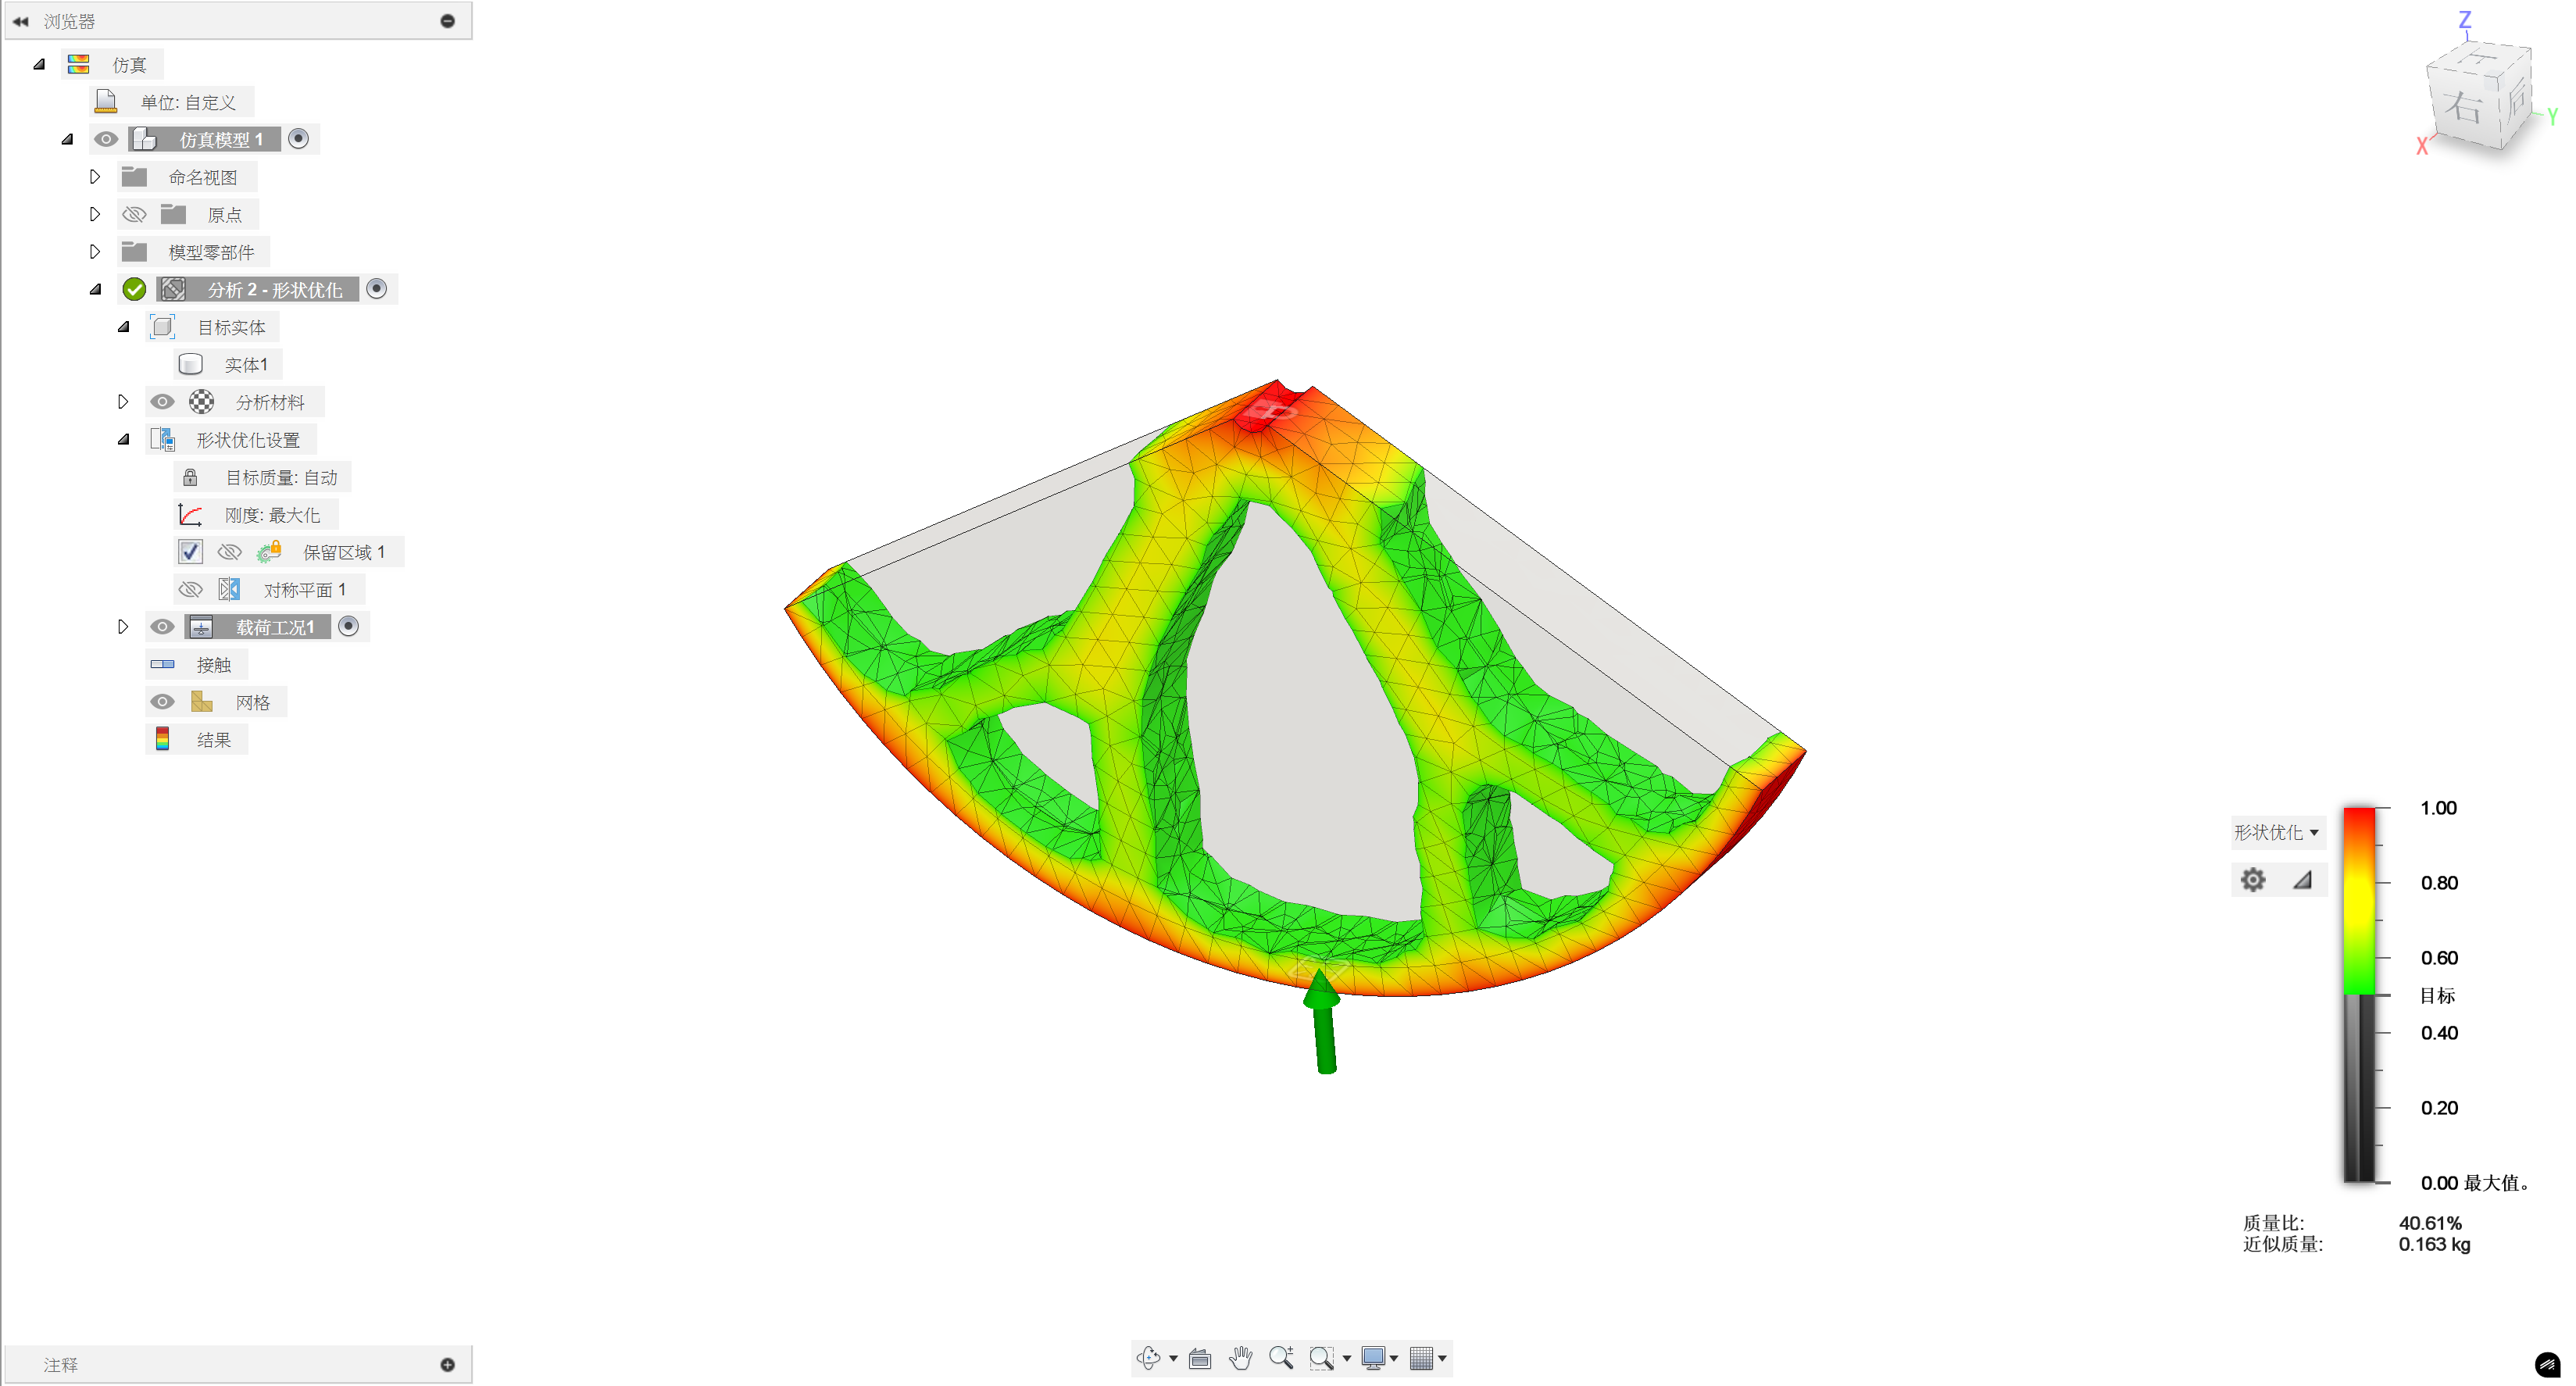
\includegraphics[width=0.7\textwidth]{46.jpg}     %圖片檔案名稱
    \caption{輪椅大輪的形狀優化2}    %圖片檔案名稱
    %如\ref{fig:example1}所示
    \label{fig:46}
\end{figure}

先用120度的扇形模擬，再做整個輪框的分析。有經過變形調整，方便可視化分析。
下圖為輪椅大輪(圖\ref{fig:47}～圖\ref{fig:49}）、輪椅側板(圖\ref{fig:50}～圖\ref{fig:52}）、小輪(圖\ref{fig:53}～圖\ref{fig:55}）的應力、應變、位移、安全係數分析。

\begin{figure}[H]
    \centering
    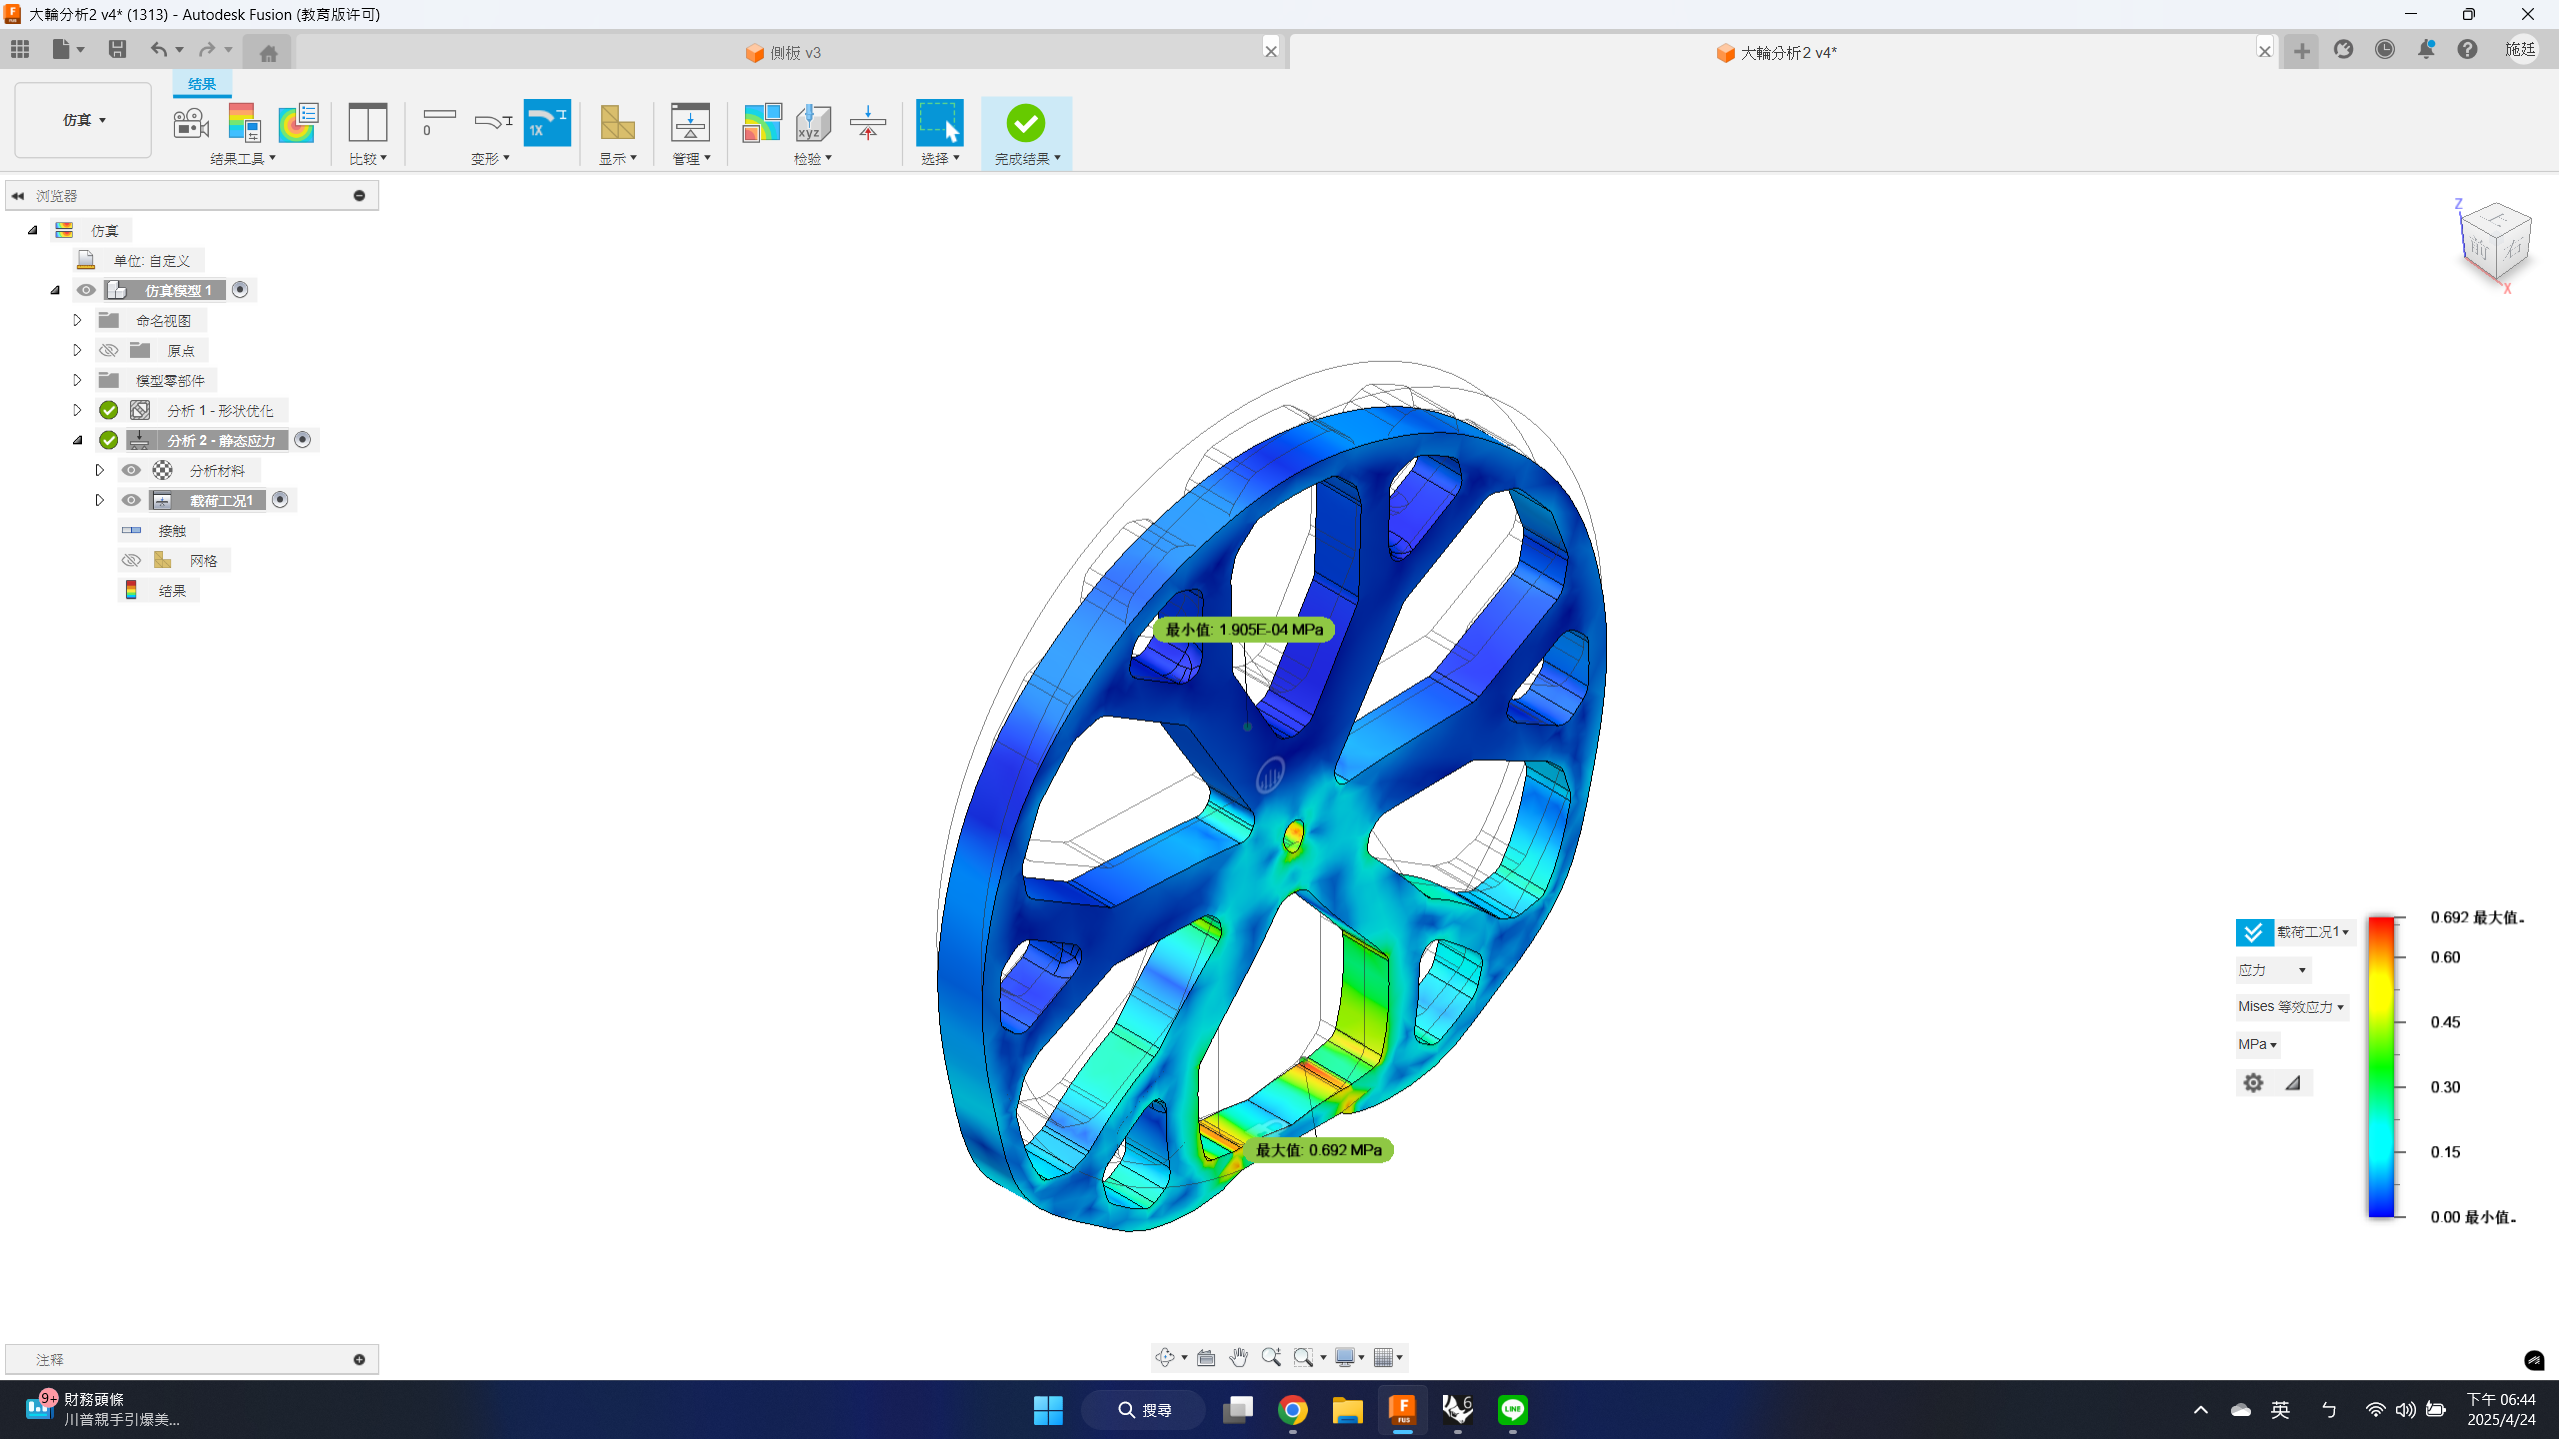
\includegraphics[width=0.7\textwidth]{47.jpg}     %圖片檔案名稱
    \caption{輪椅大輪的應變分析}    %圖片檔案名稱
    %如\ref{fig:example1}所示
    \label{fig:47}
\end{figure}

\begin{figure}[H]
    \centering
    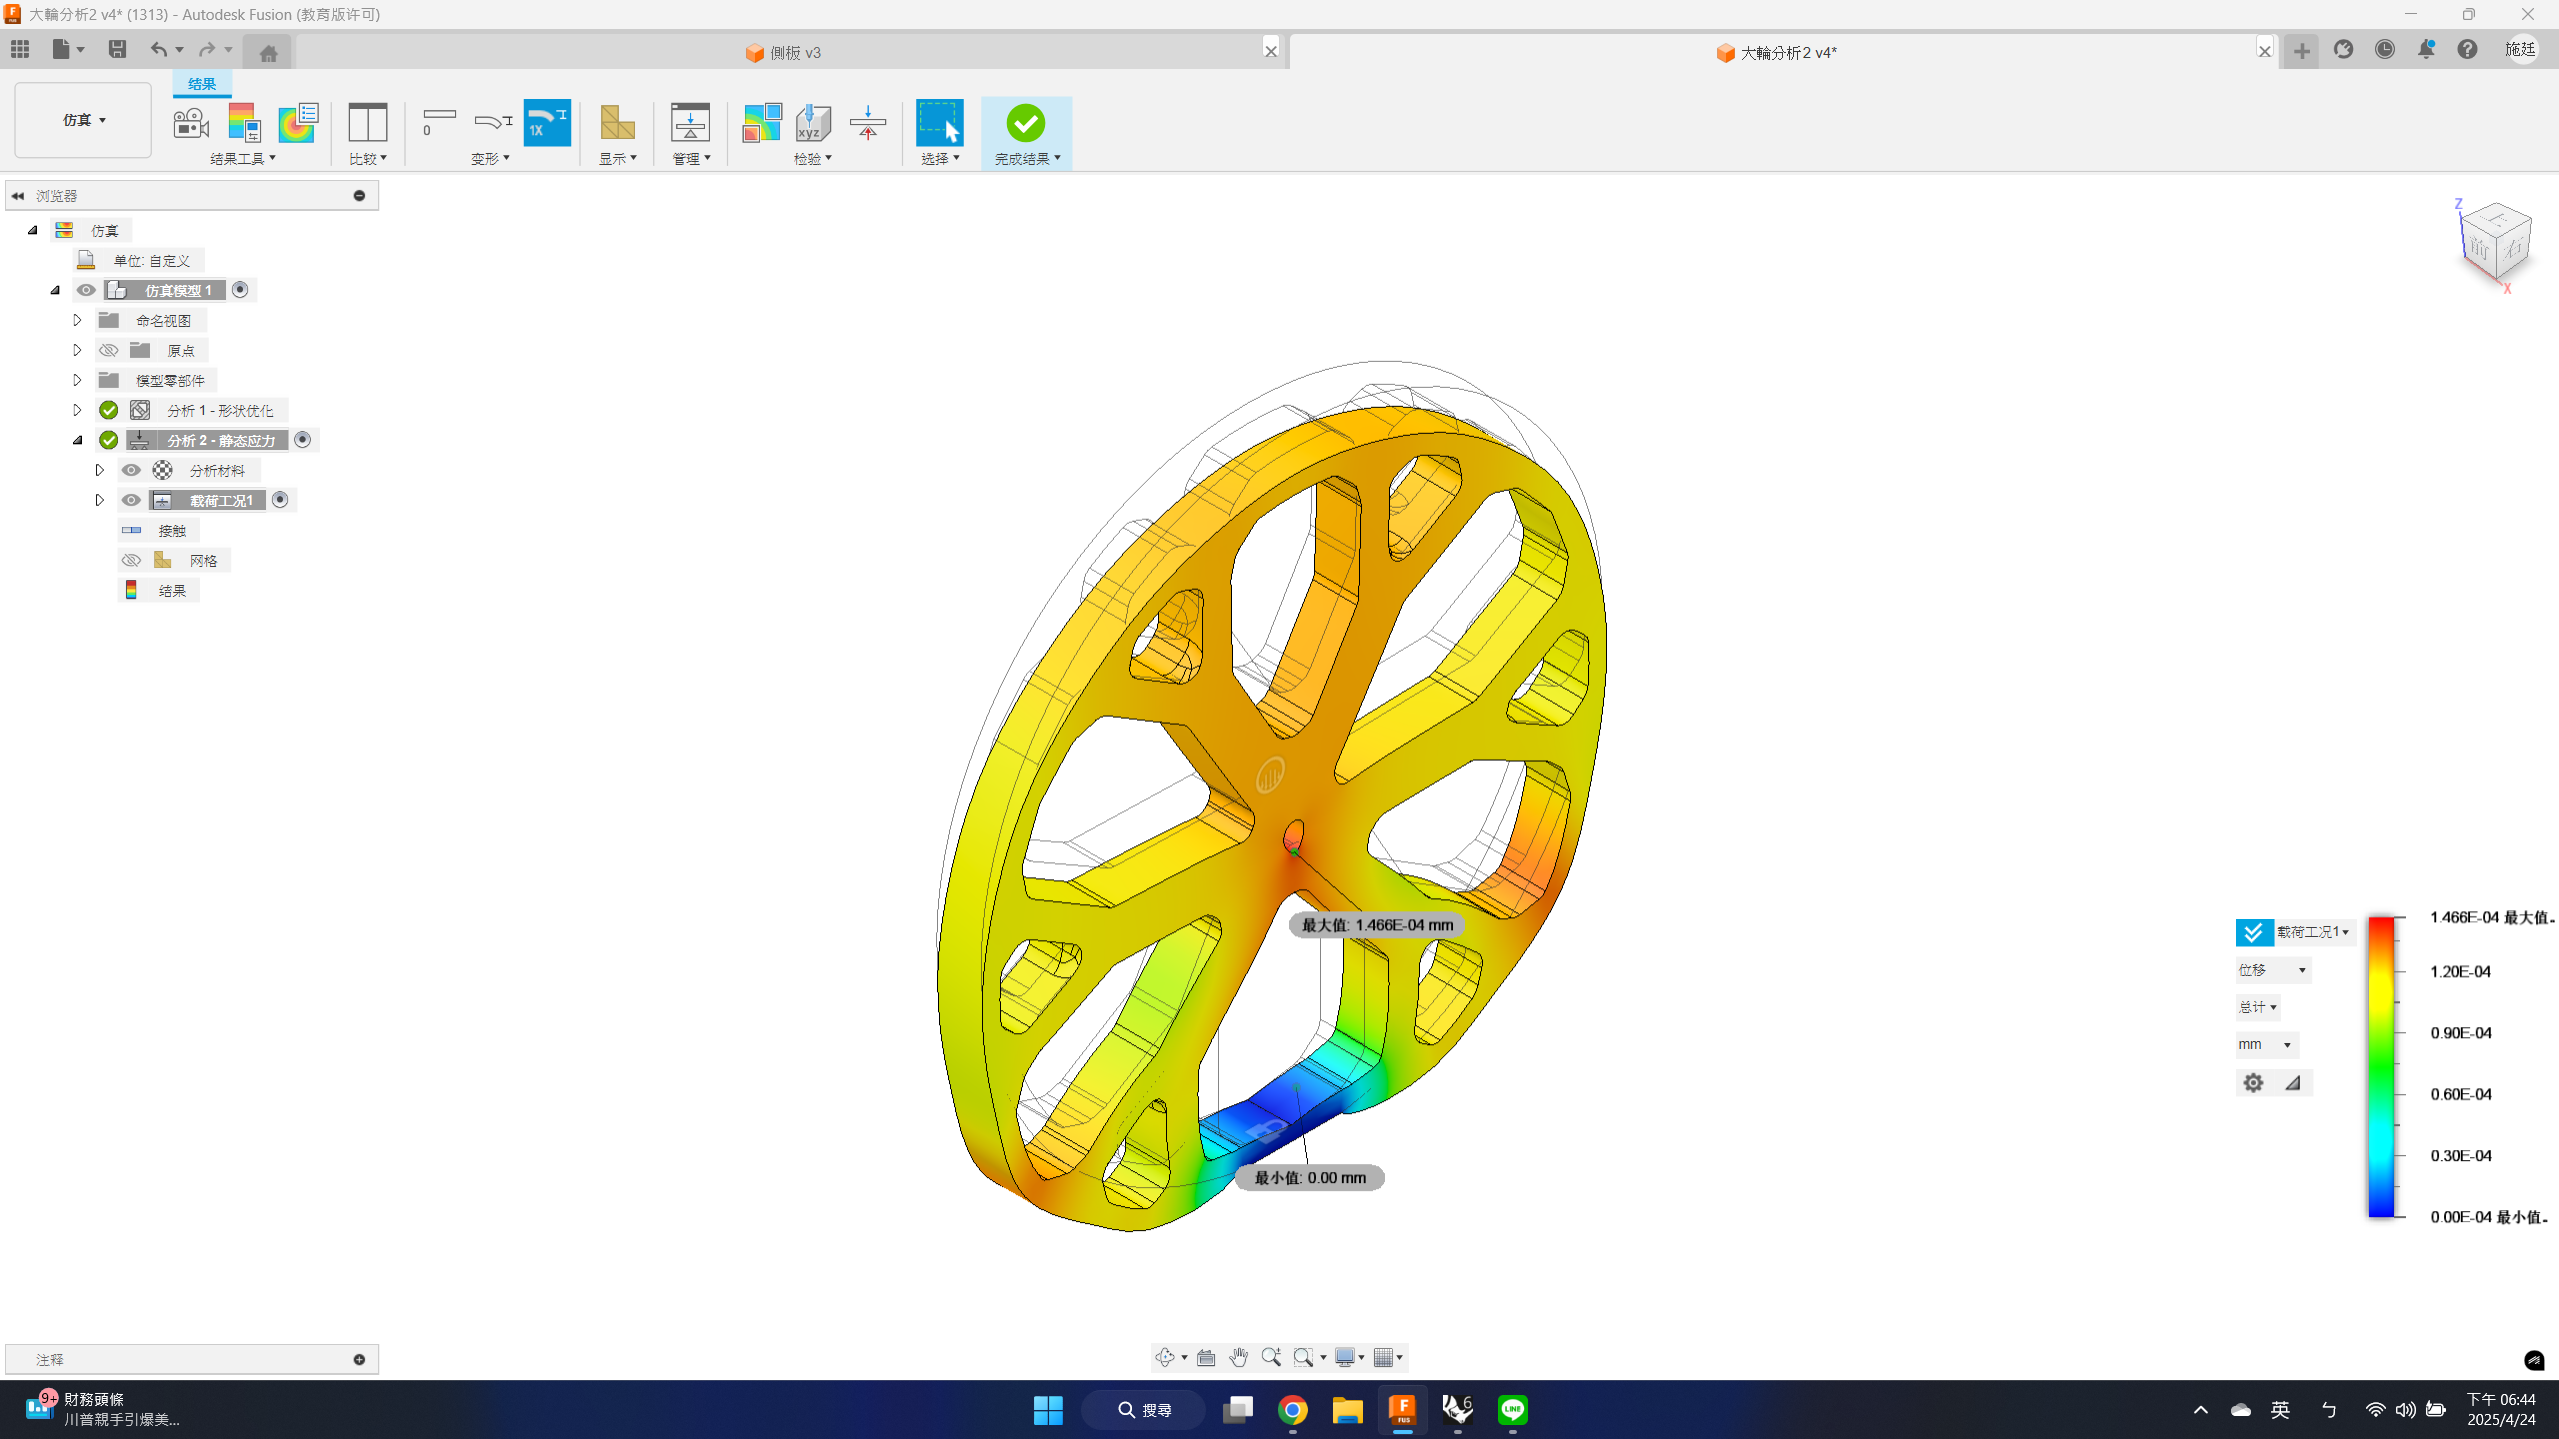
\includegraphics[width=0.7\textwidth]{48.jpg}     %圖片檔案名稱
    \caption{輪椅大輪的位移分析}    %圖片檔案名稱
    %如\ref{fig:example1}所示
\end{figure}

\begin{figure}[H]
    \centering
    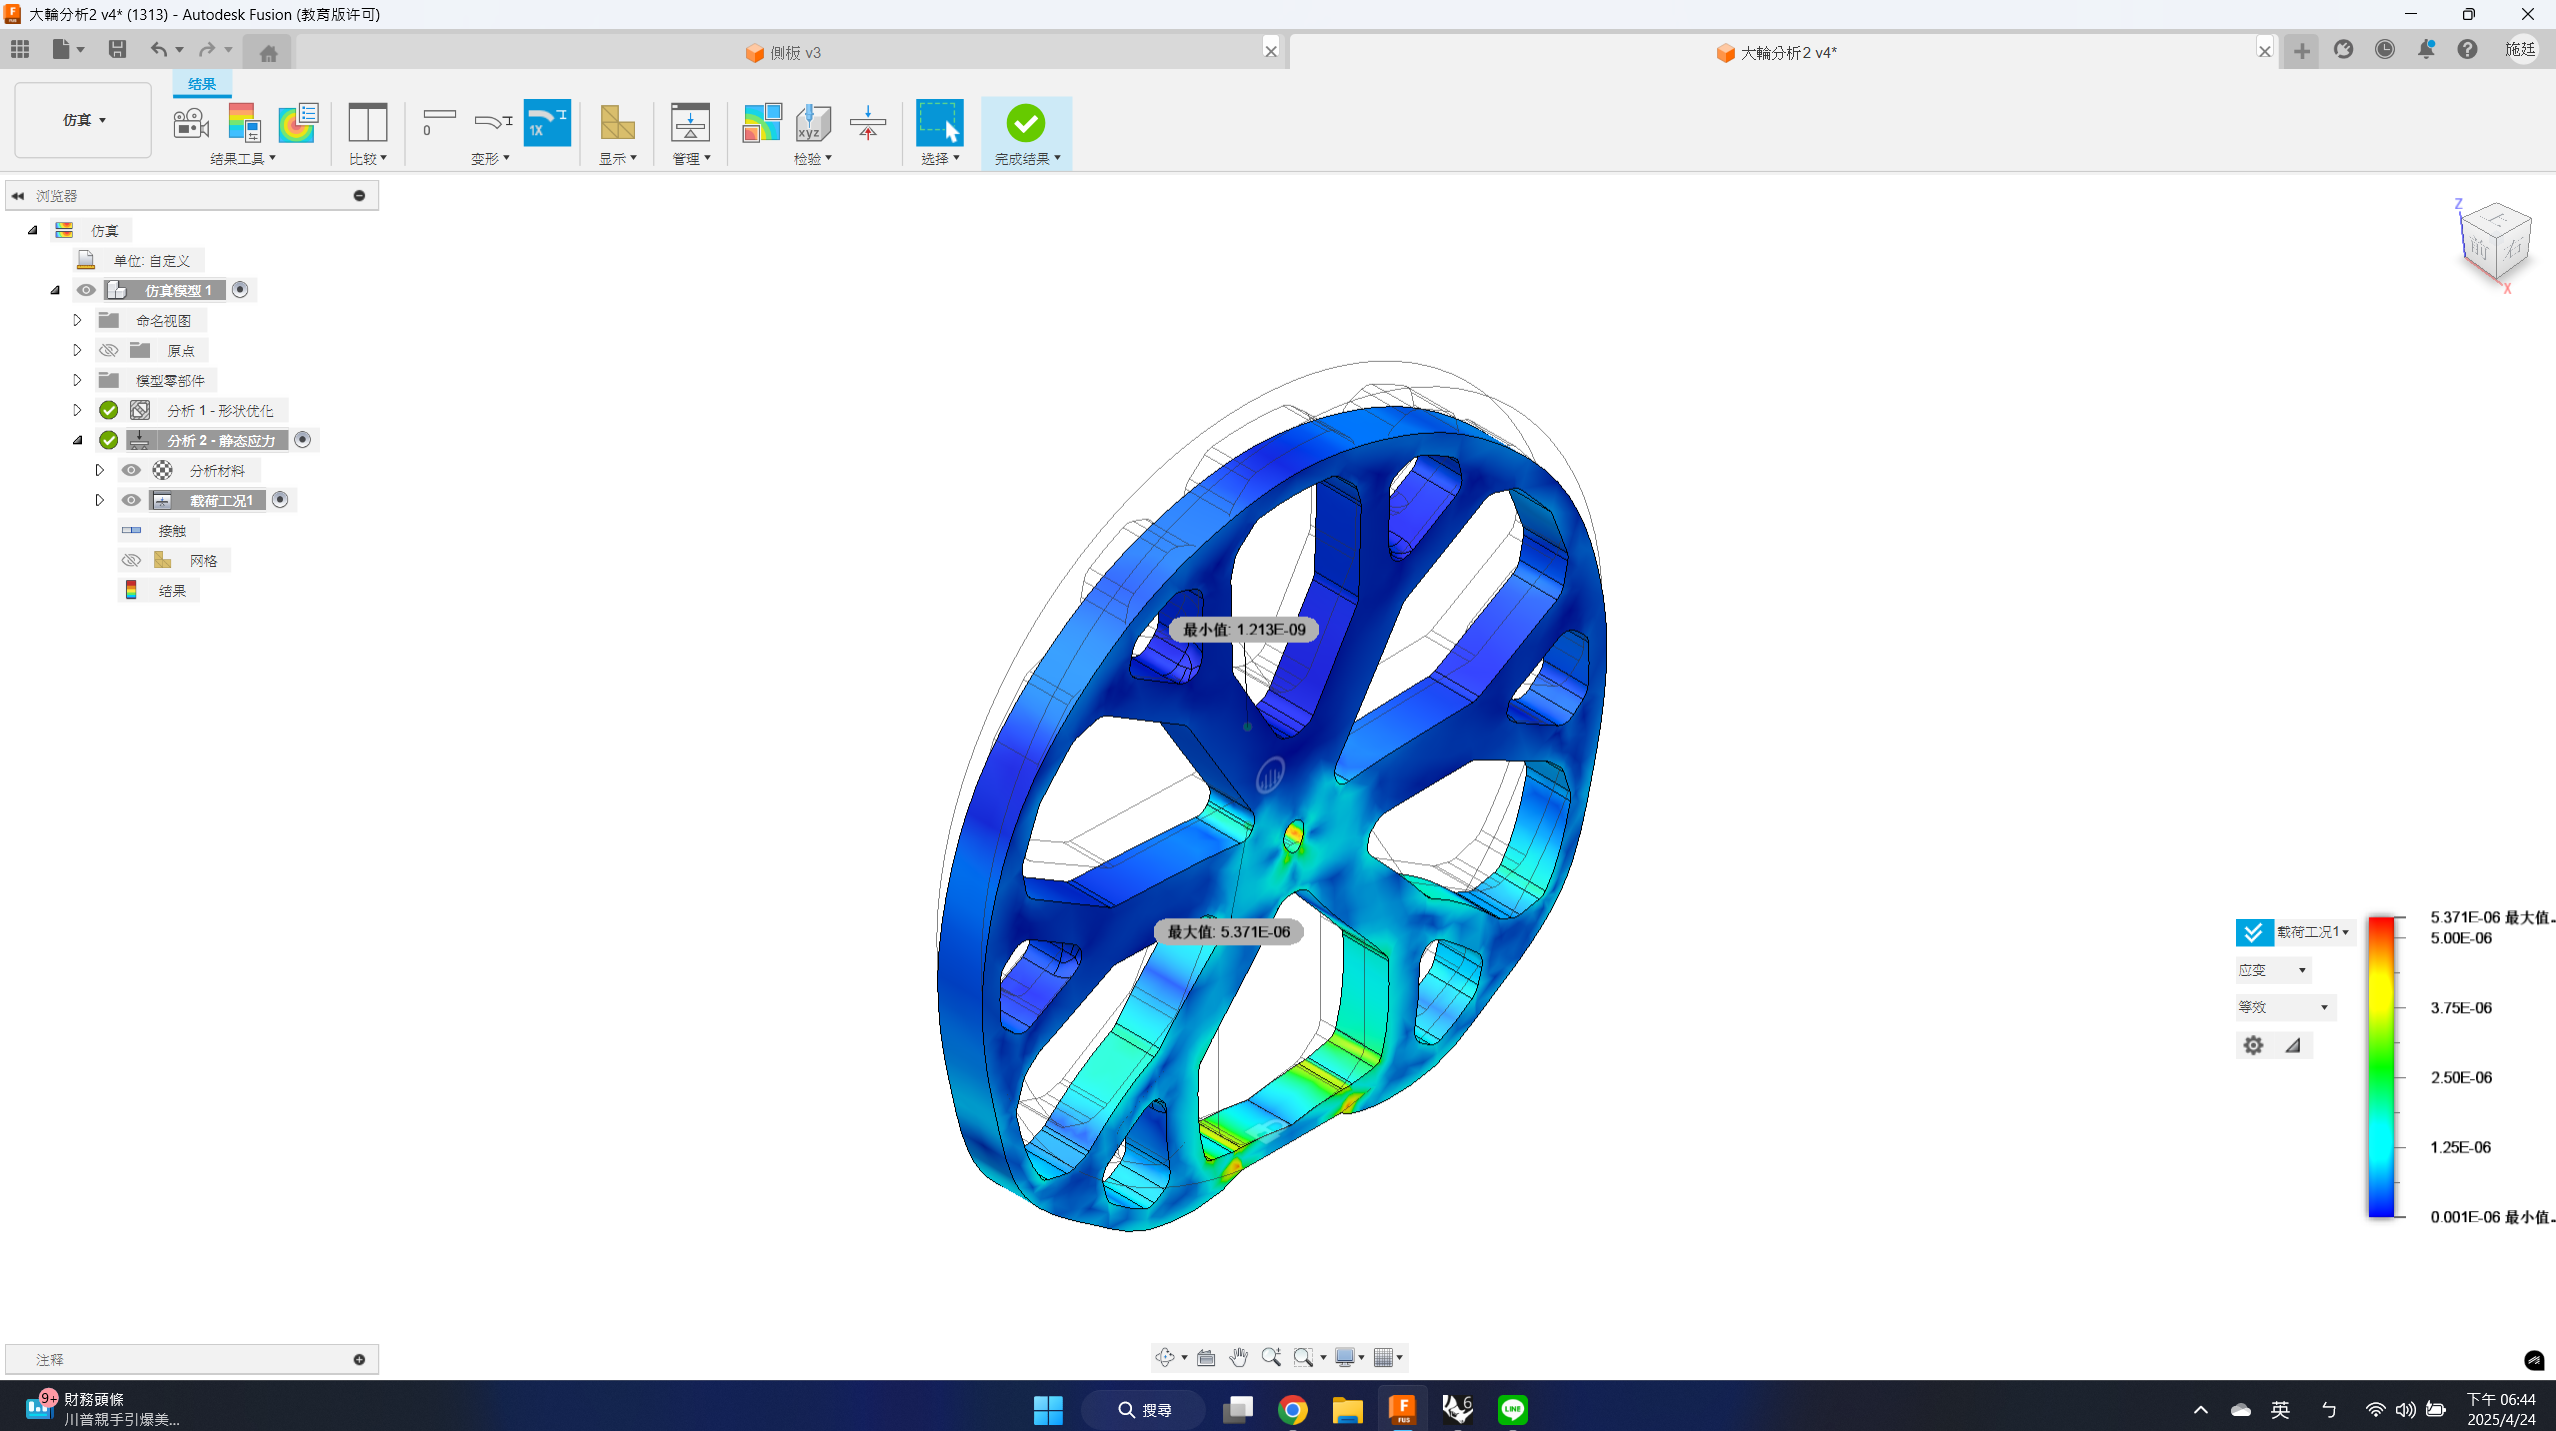
\includegraphics[width=0.7\textwidth]{49.jpg}     %圖片檔案名稱
    \caption{輪椅大輪的應力分析}    %圖片檔案名稱
    %如\ref{fig:example1}所示
    \label{fig:49}
\end{figure}

\begin{figure}[H]
    \centering
    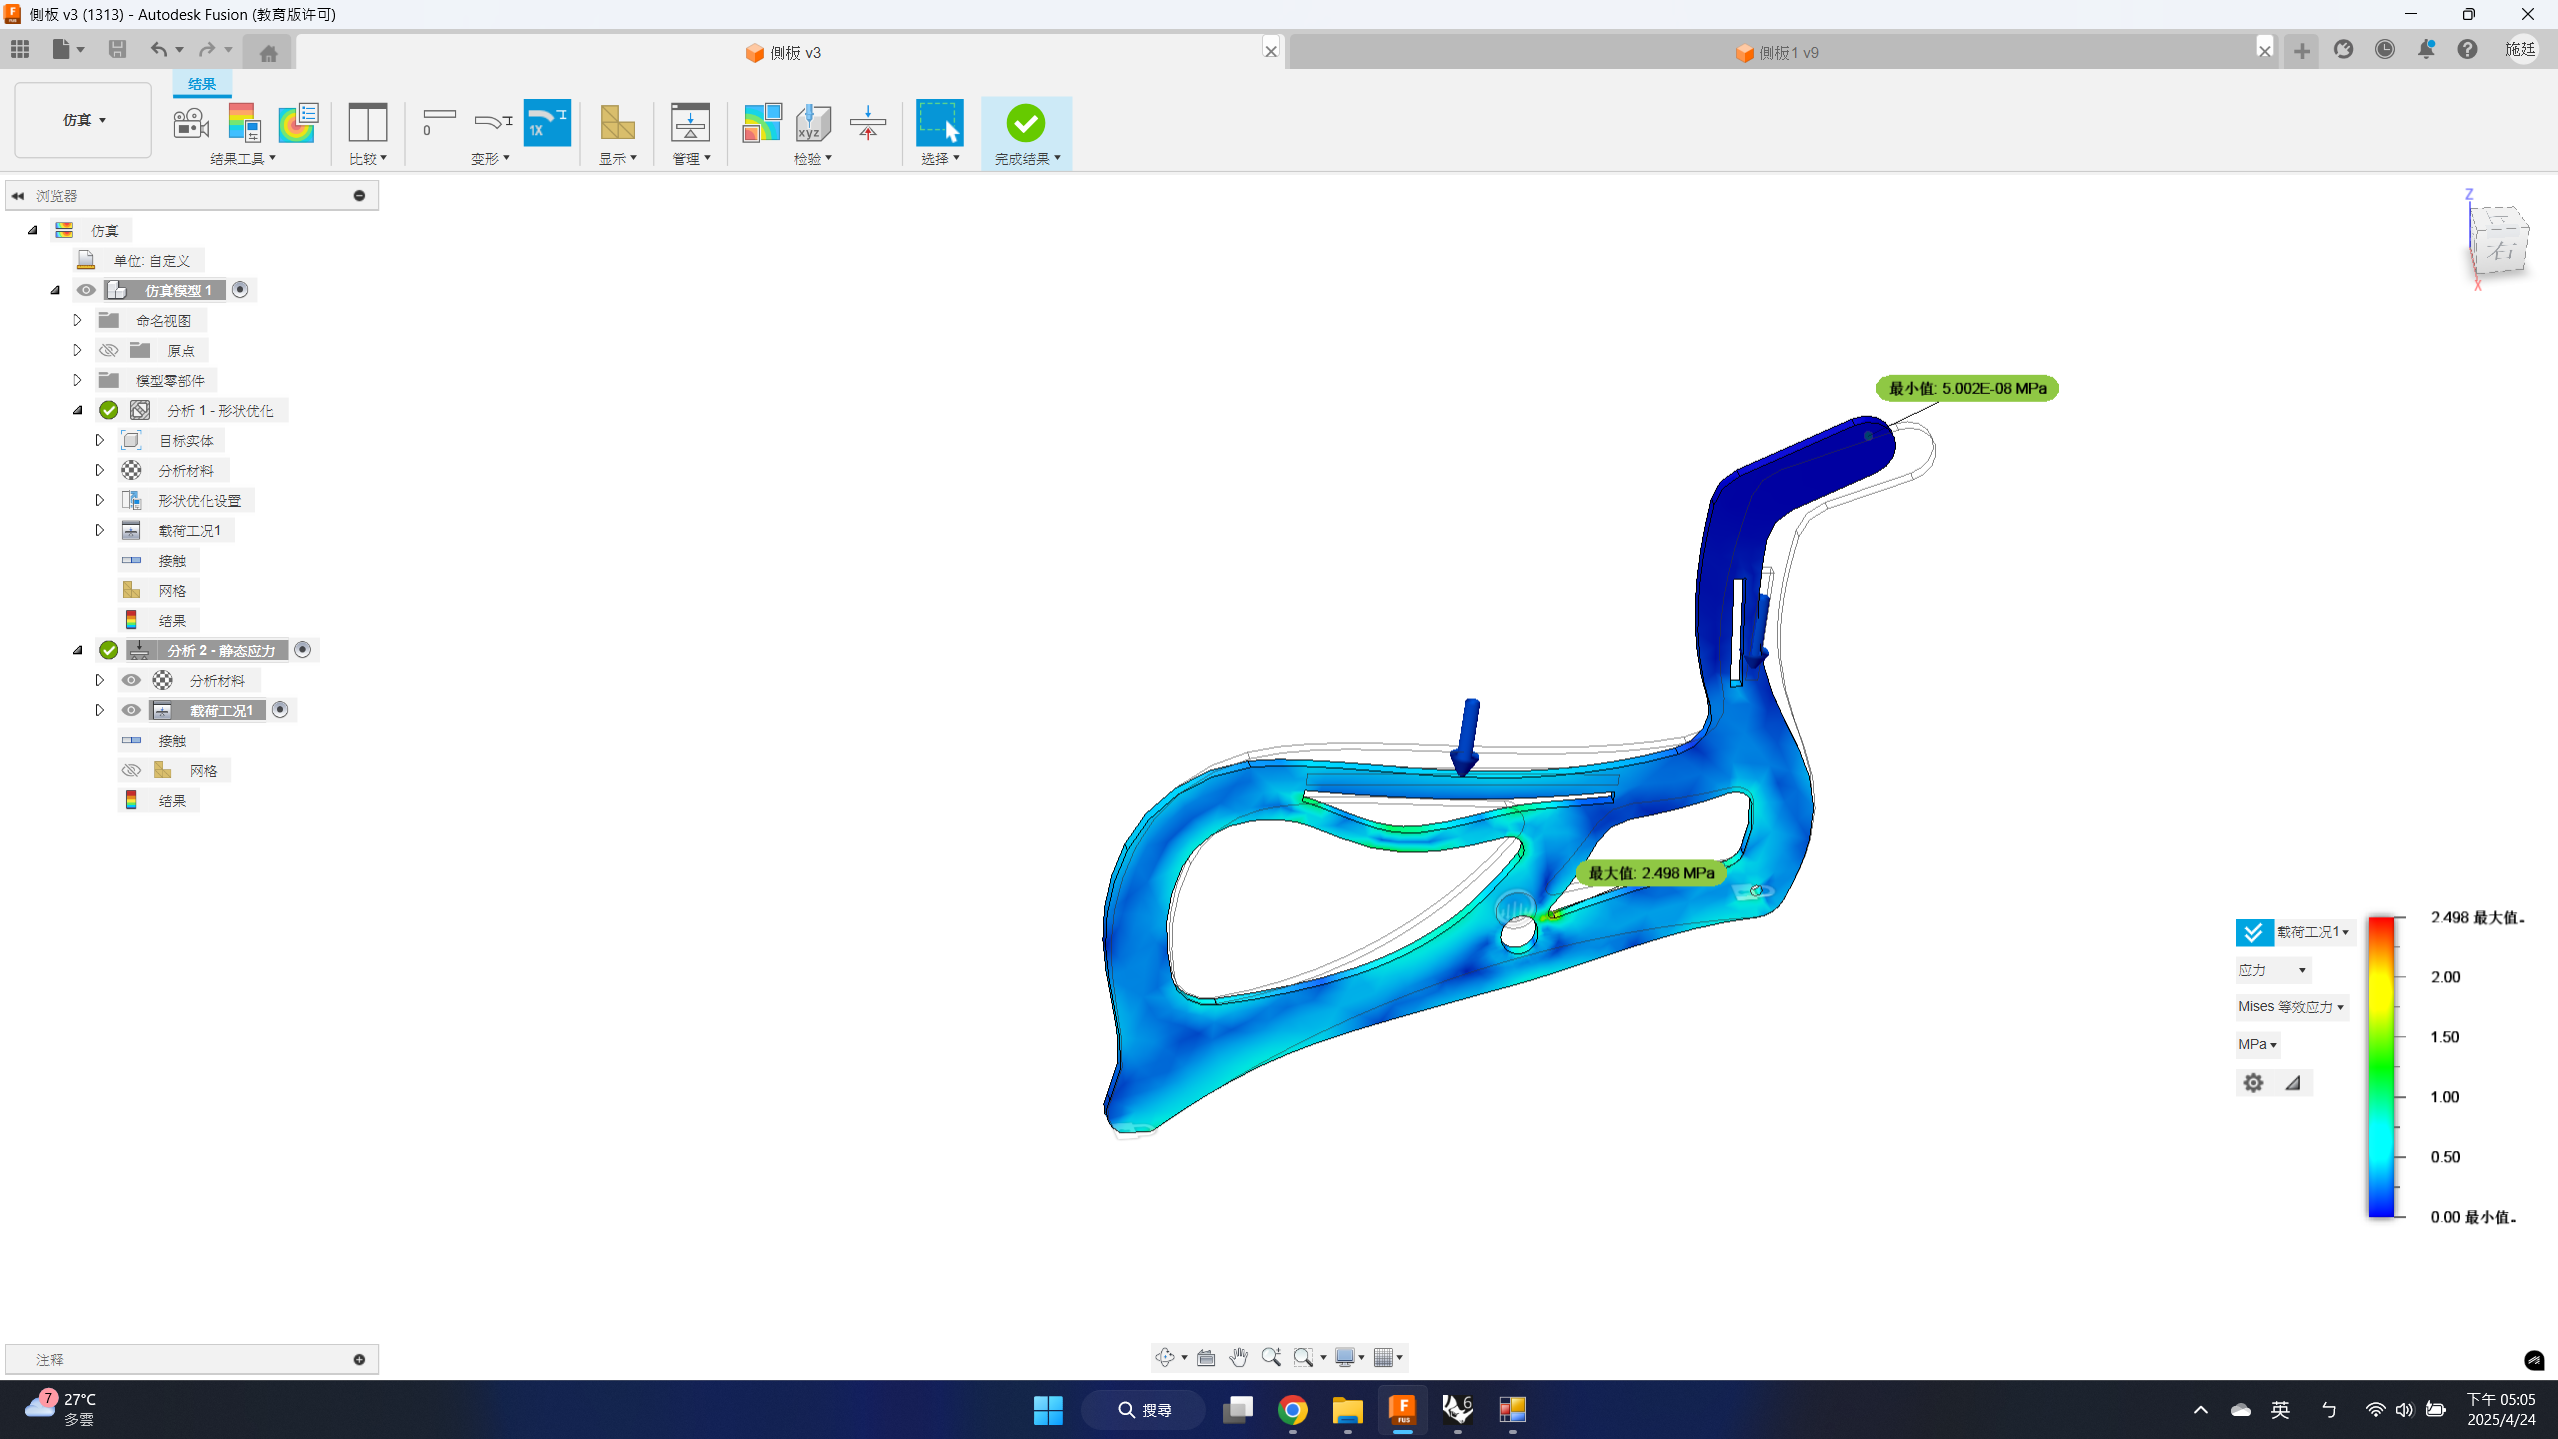
\includegraphics[width=0.7\textwidth]{50.jpg}     %圖片檔案名稱
    \caption{輪椅側板的應力分析}    %圖片檔案名稱
    %如\ref{fig:example1}所示
    \label{fig:50}
\end{figure}

\begin{figure}[H]
    \centering
    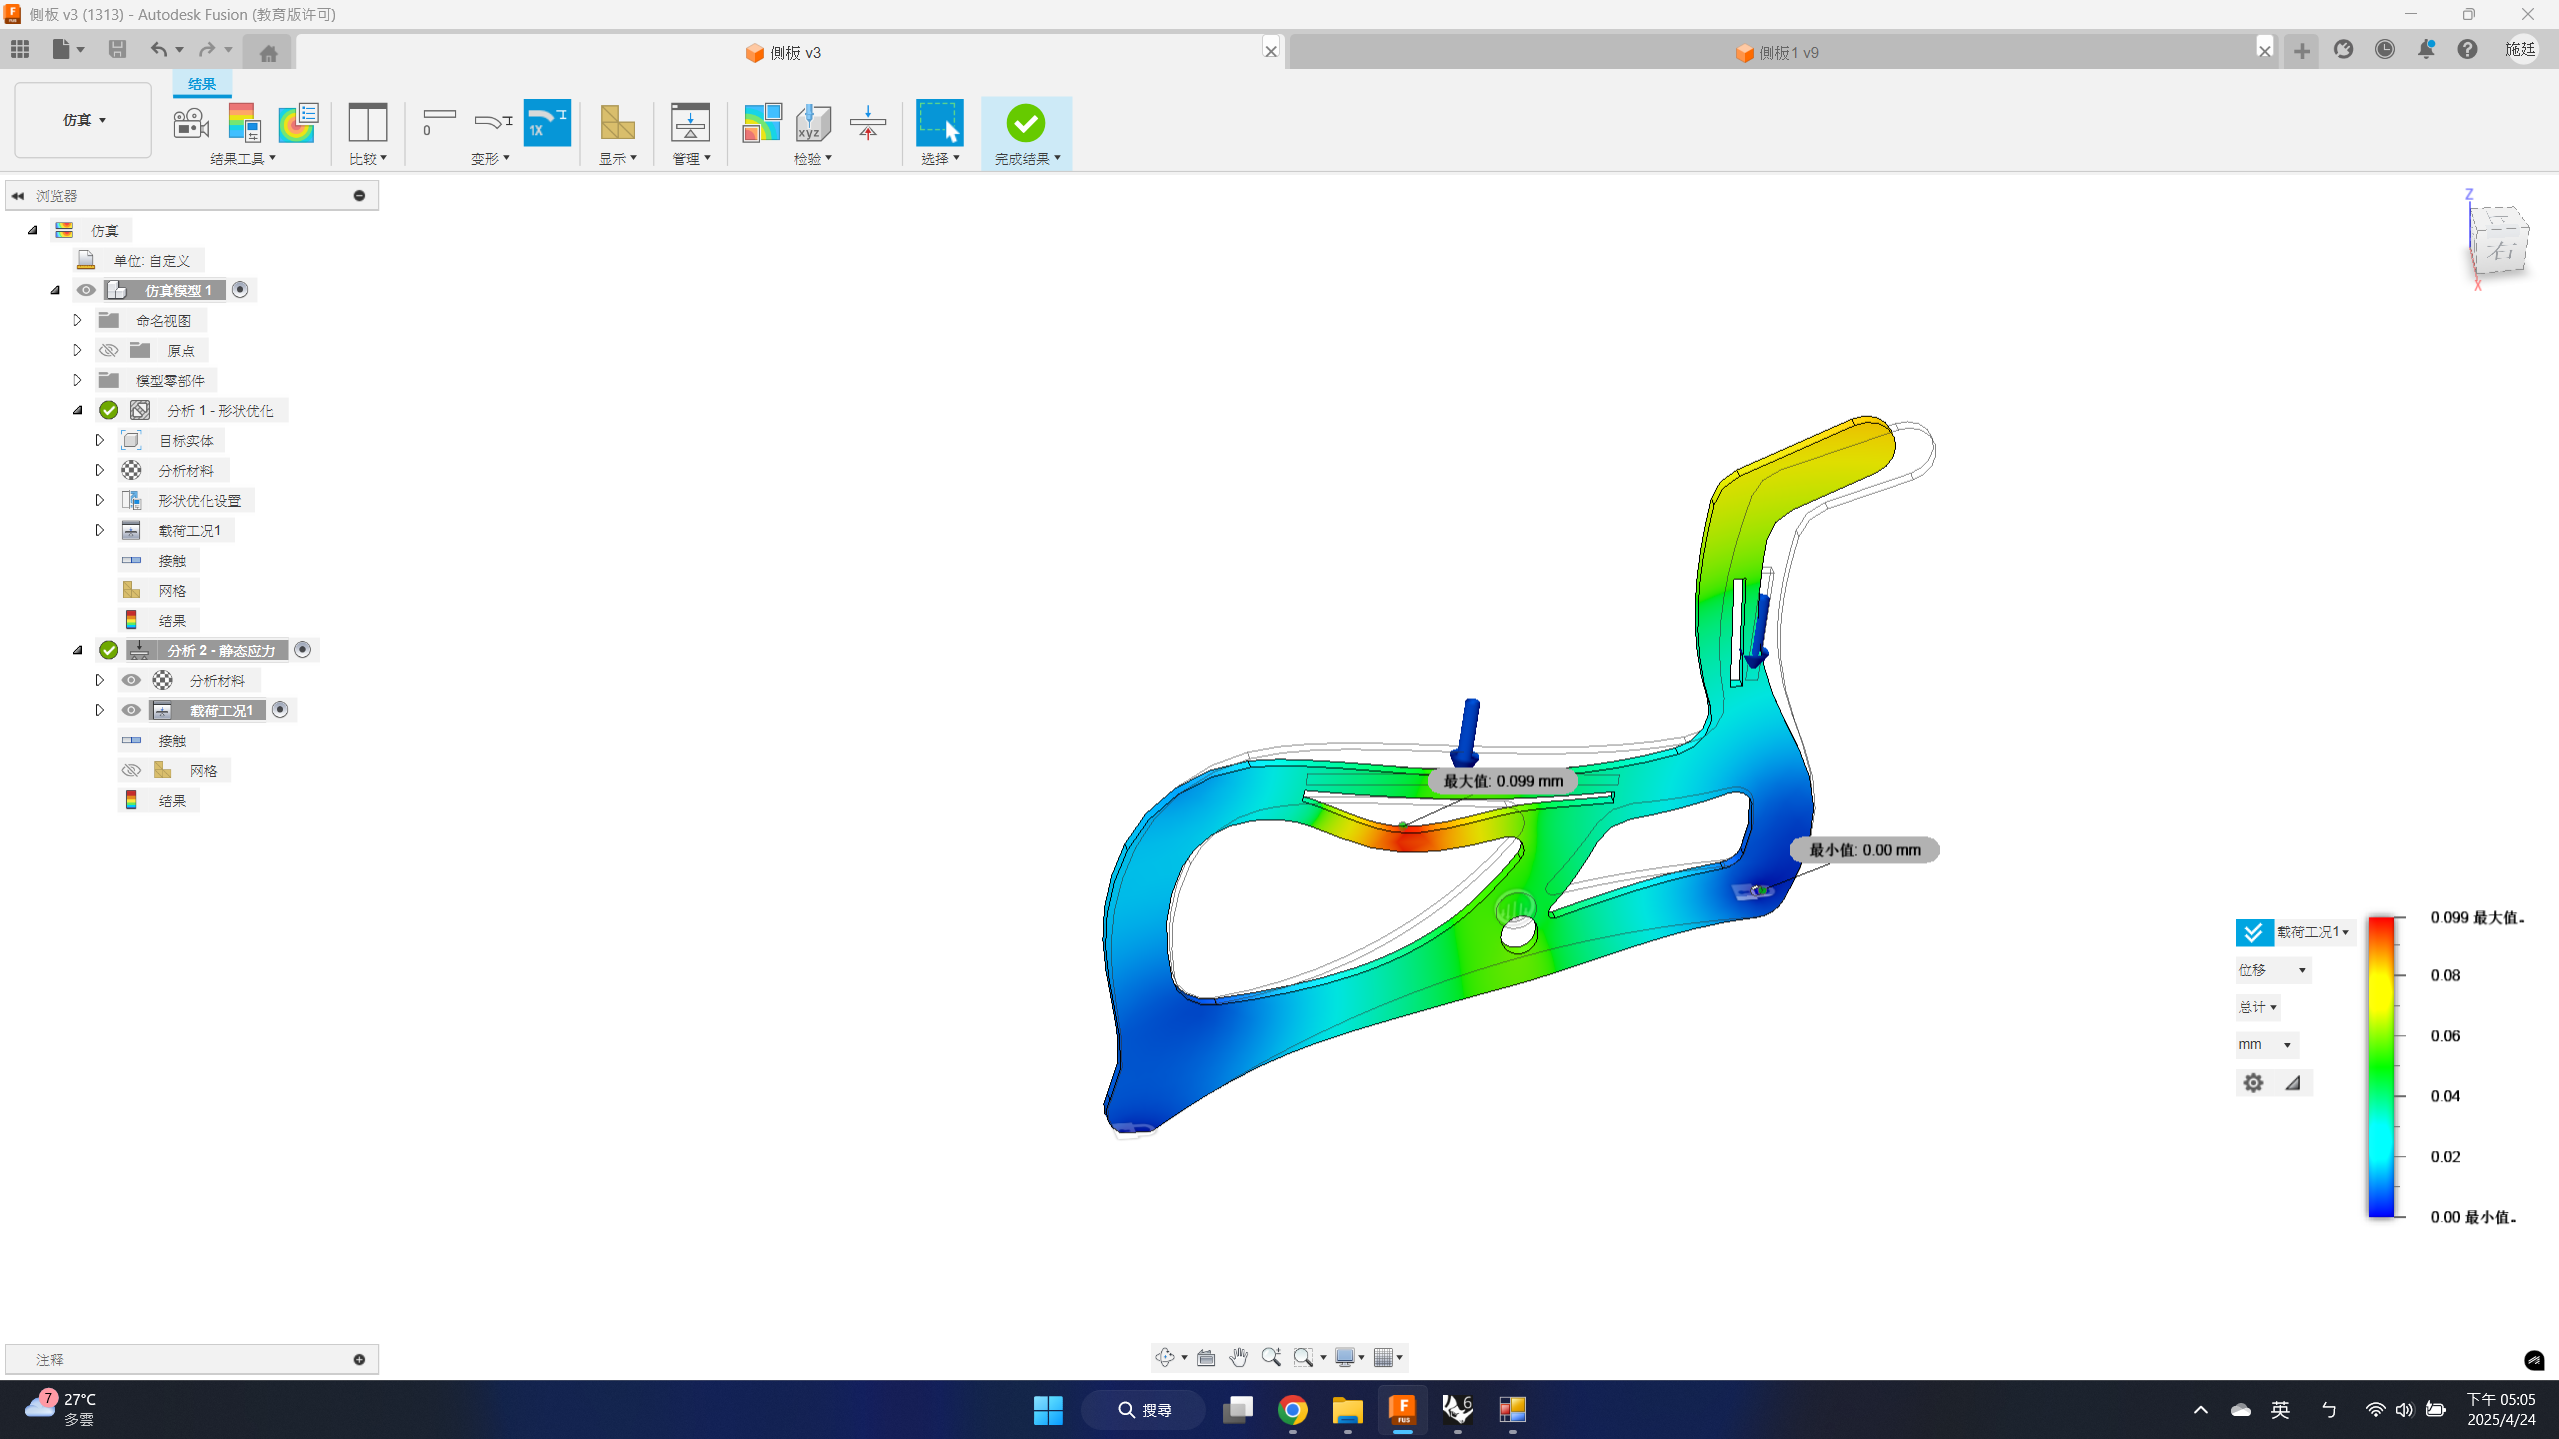
\includegraphics[width=0.7\textwidth]{51.jpg}     %圖片檔案名稱
    \caption{輪椅側板的位移分析}    %圖片檔案名稱
    %如\ref{fig:example1}所示
\end{figure}

\begin{figure}[H]
    \centering
    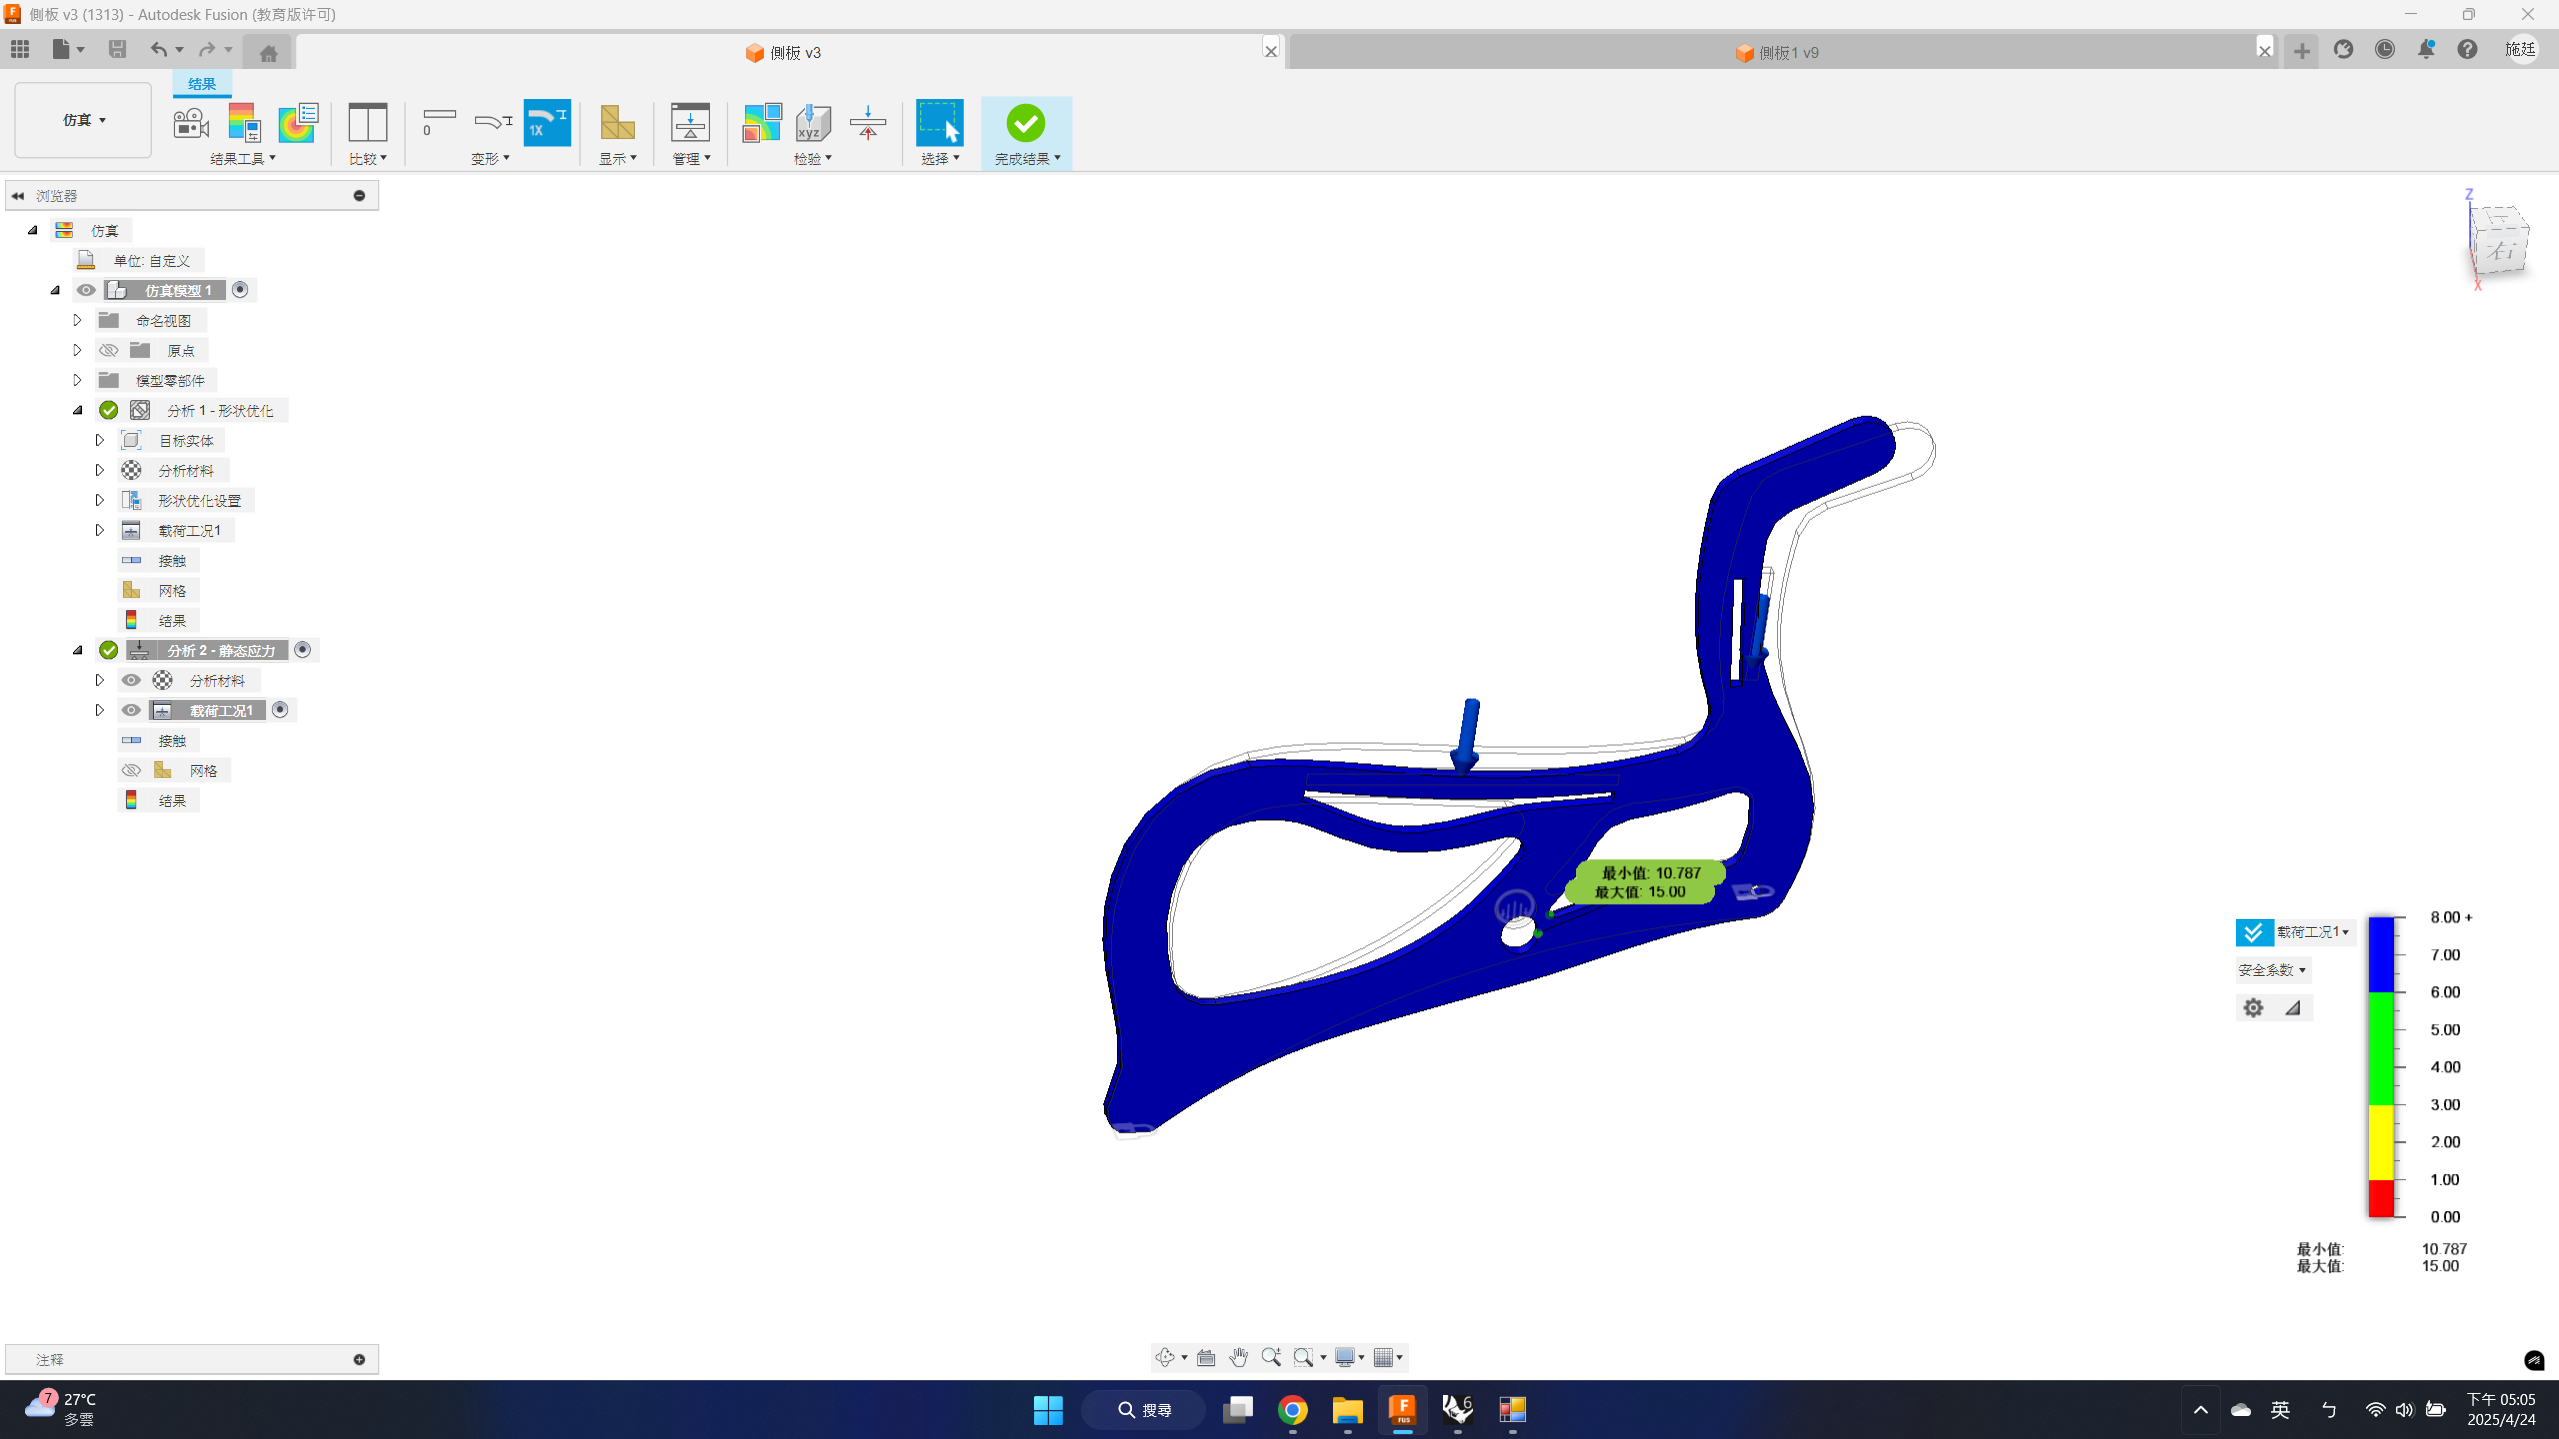
\includegraphics[width=0.7\textwidth]{52.jpg}     %圖片檔案名稱
    \caption{輪椅側板的安全係數分析}    %圖片檔案名稱
    %如\ref{fig:example1}所示
    \label{fig:52}
\end{figure}

\begin{figure}[H]
    \centering
    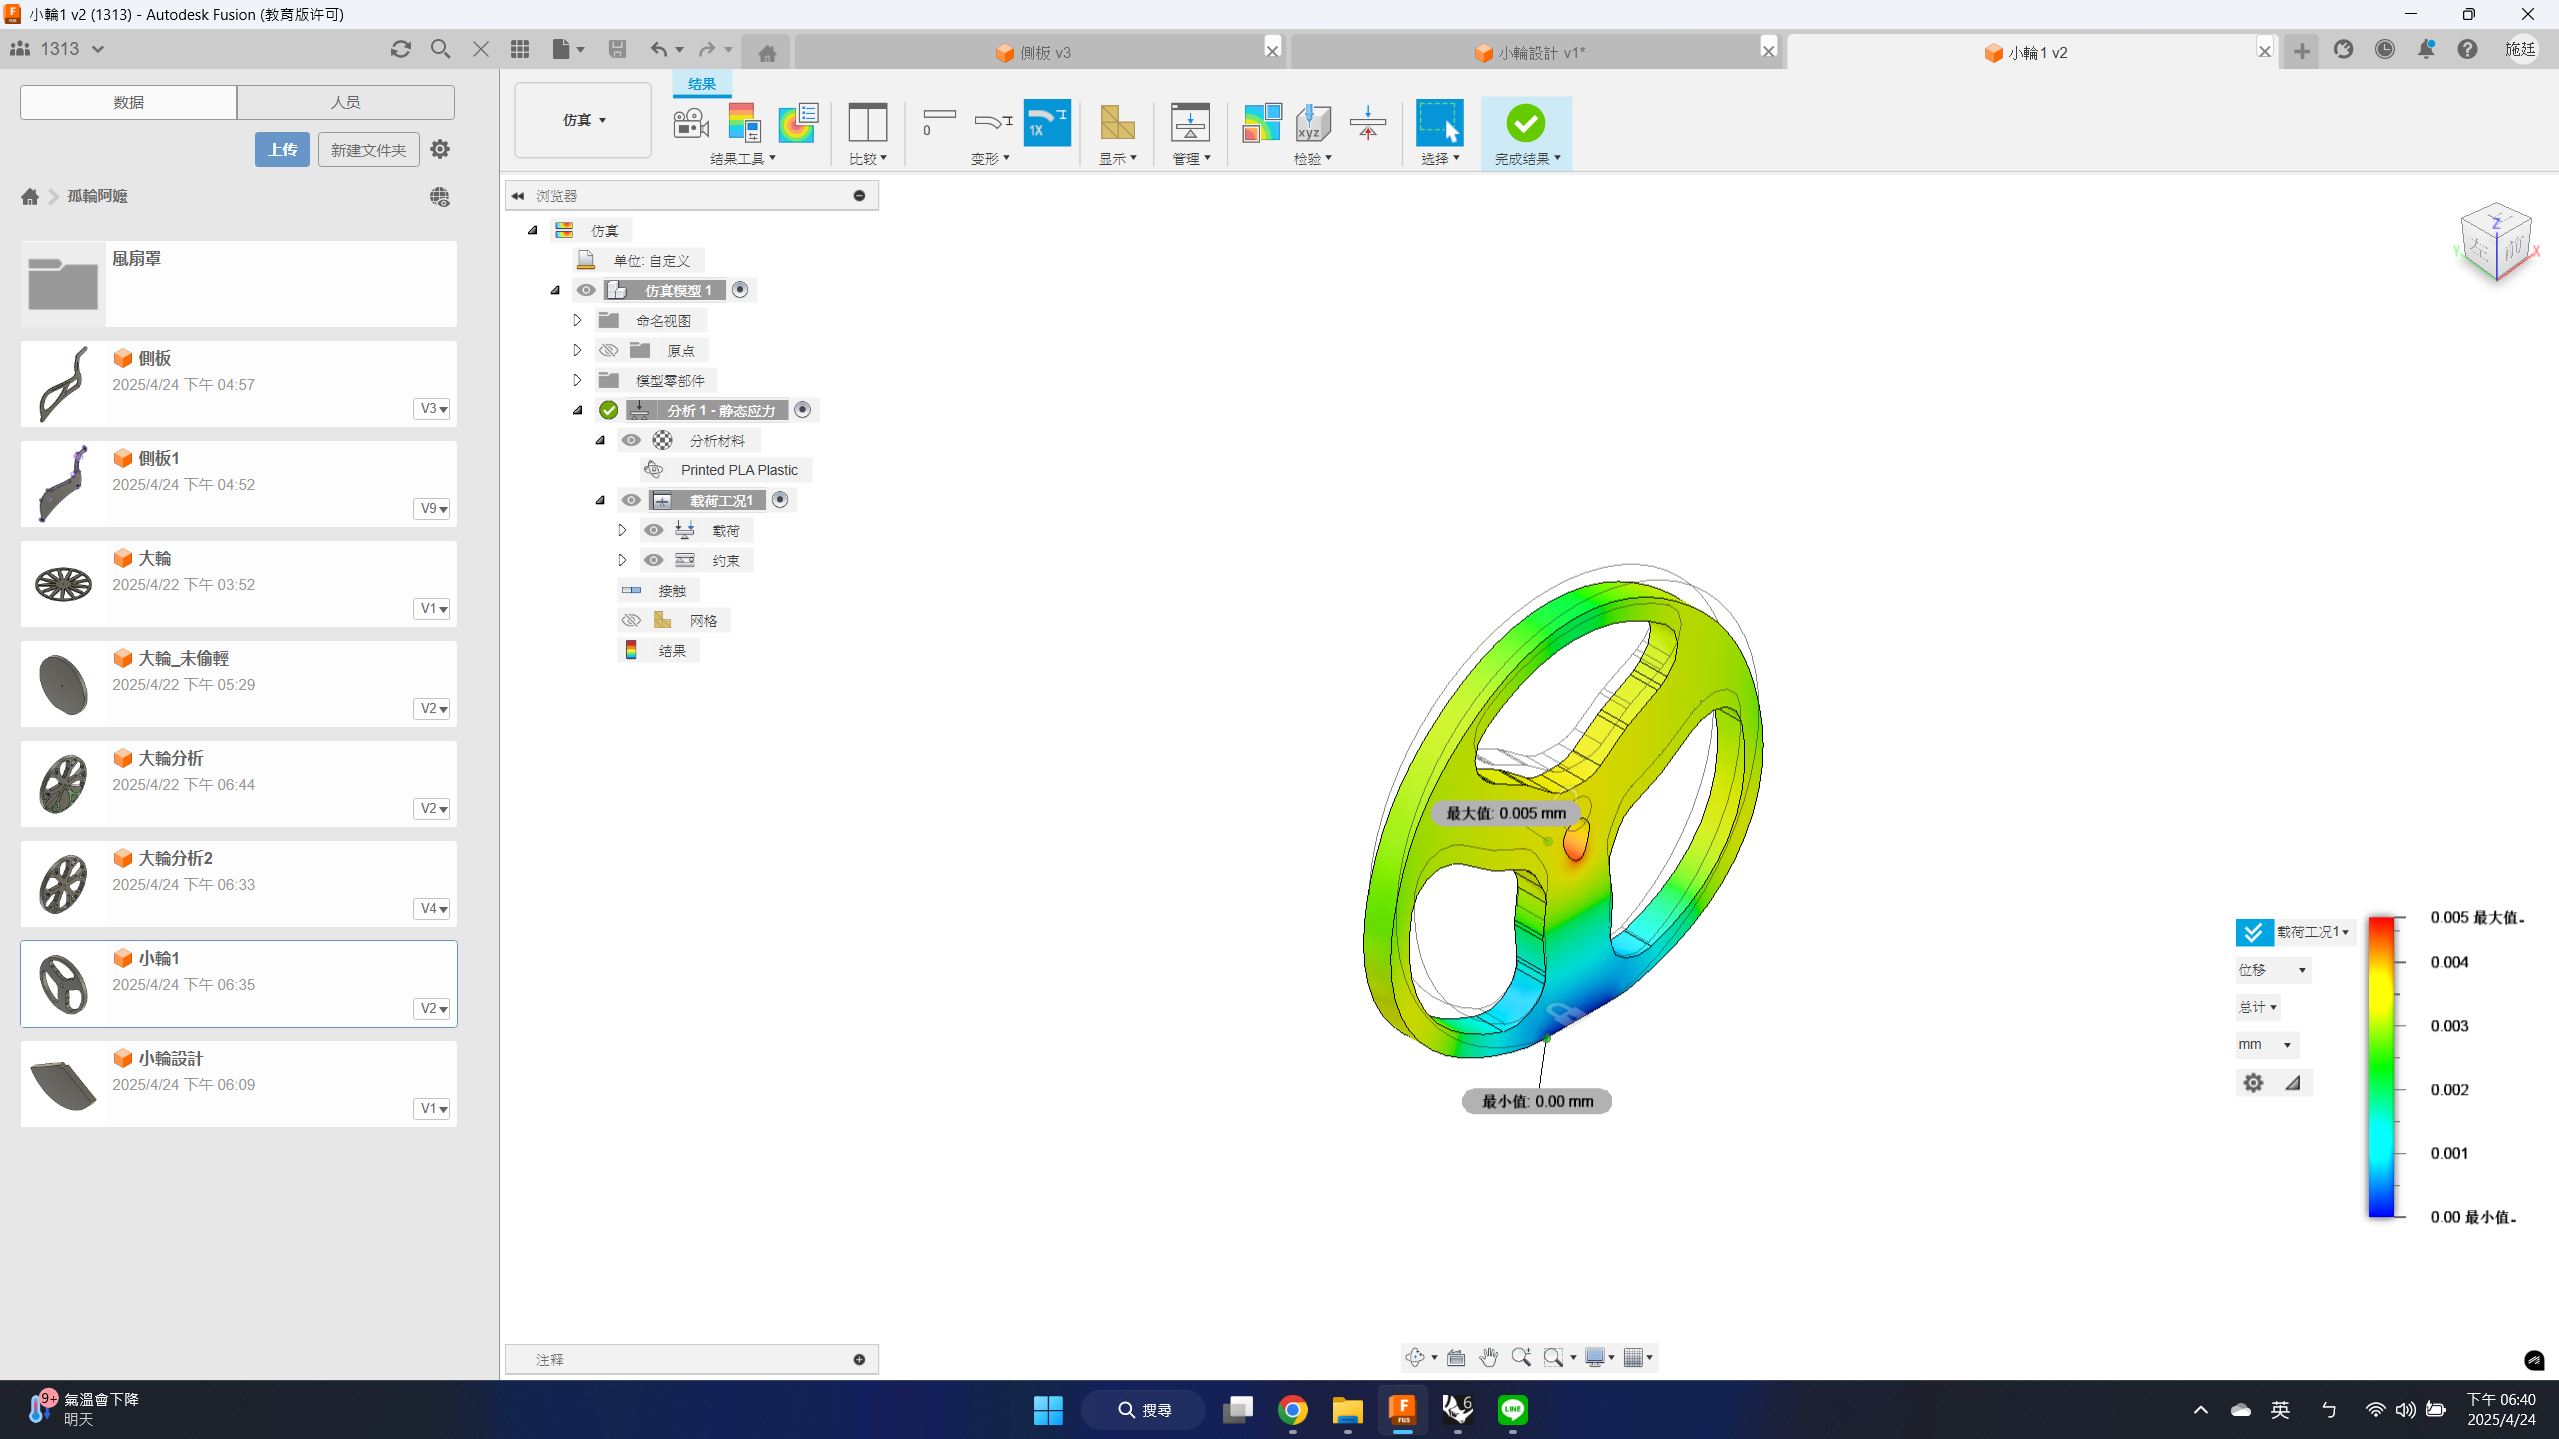
\includegraphics[width=0.7\textwidth]{53.jpg}     %圖片檔案名稱
    \caption{小輪的位移分析}    %圖片檔案名稱
    %如\ref{fig:example1}所示
    \label{fig:53}
\end{figure}

\begin{figure}[H]
    \centering
    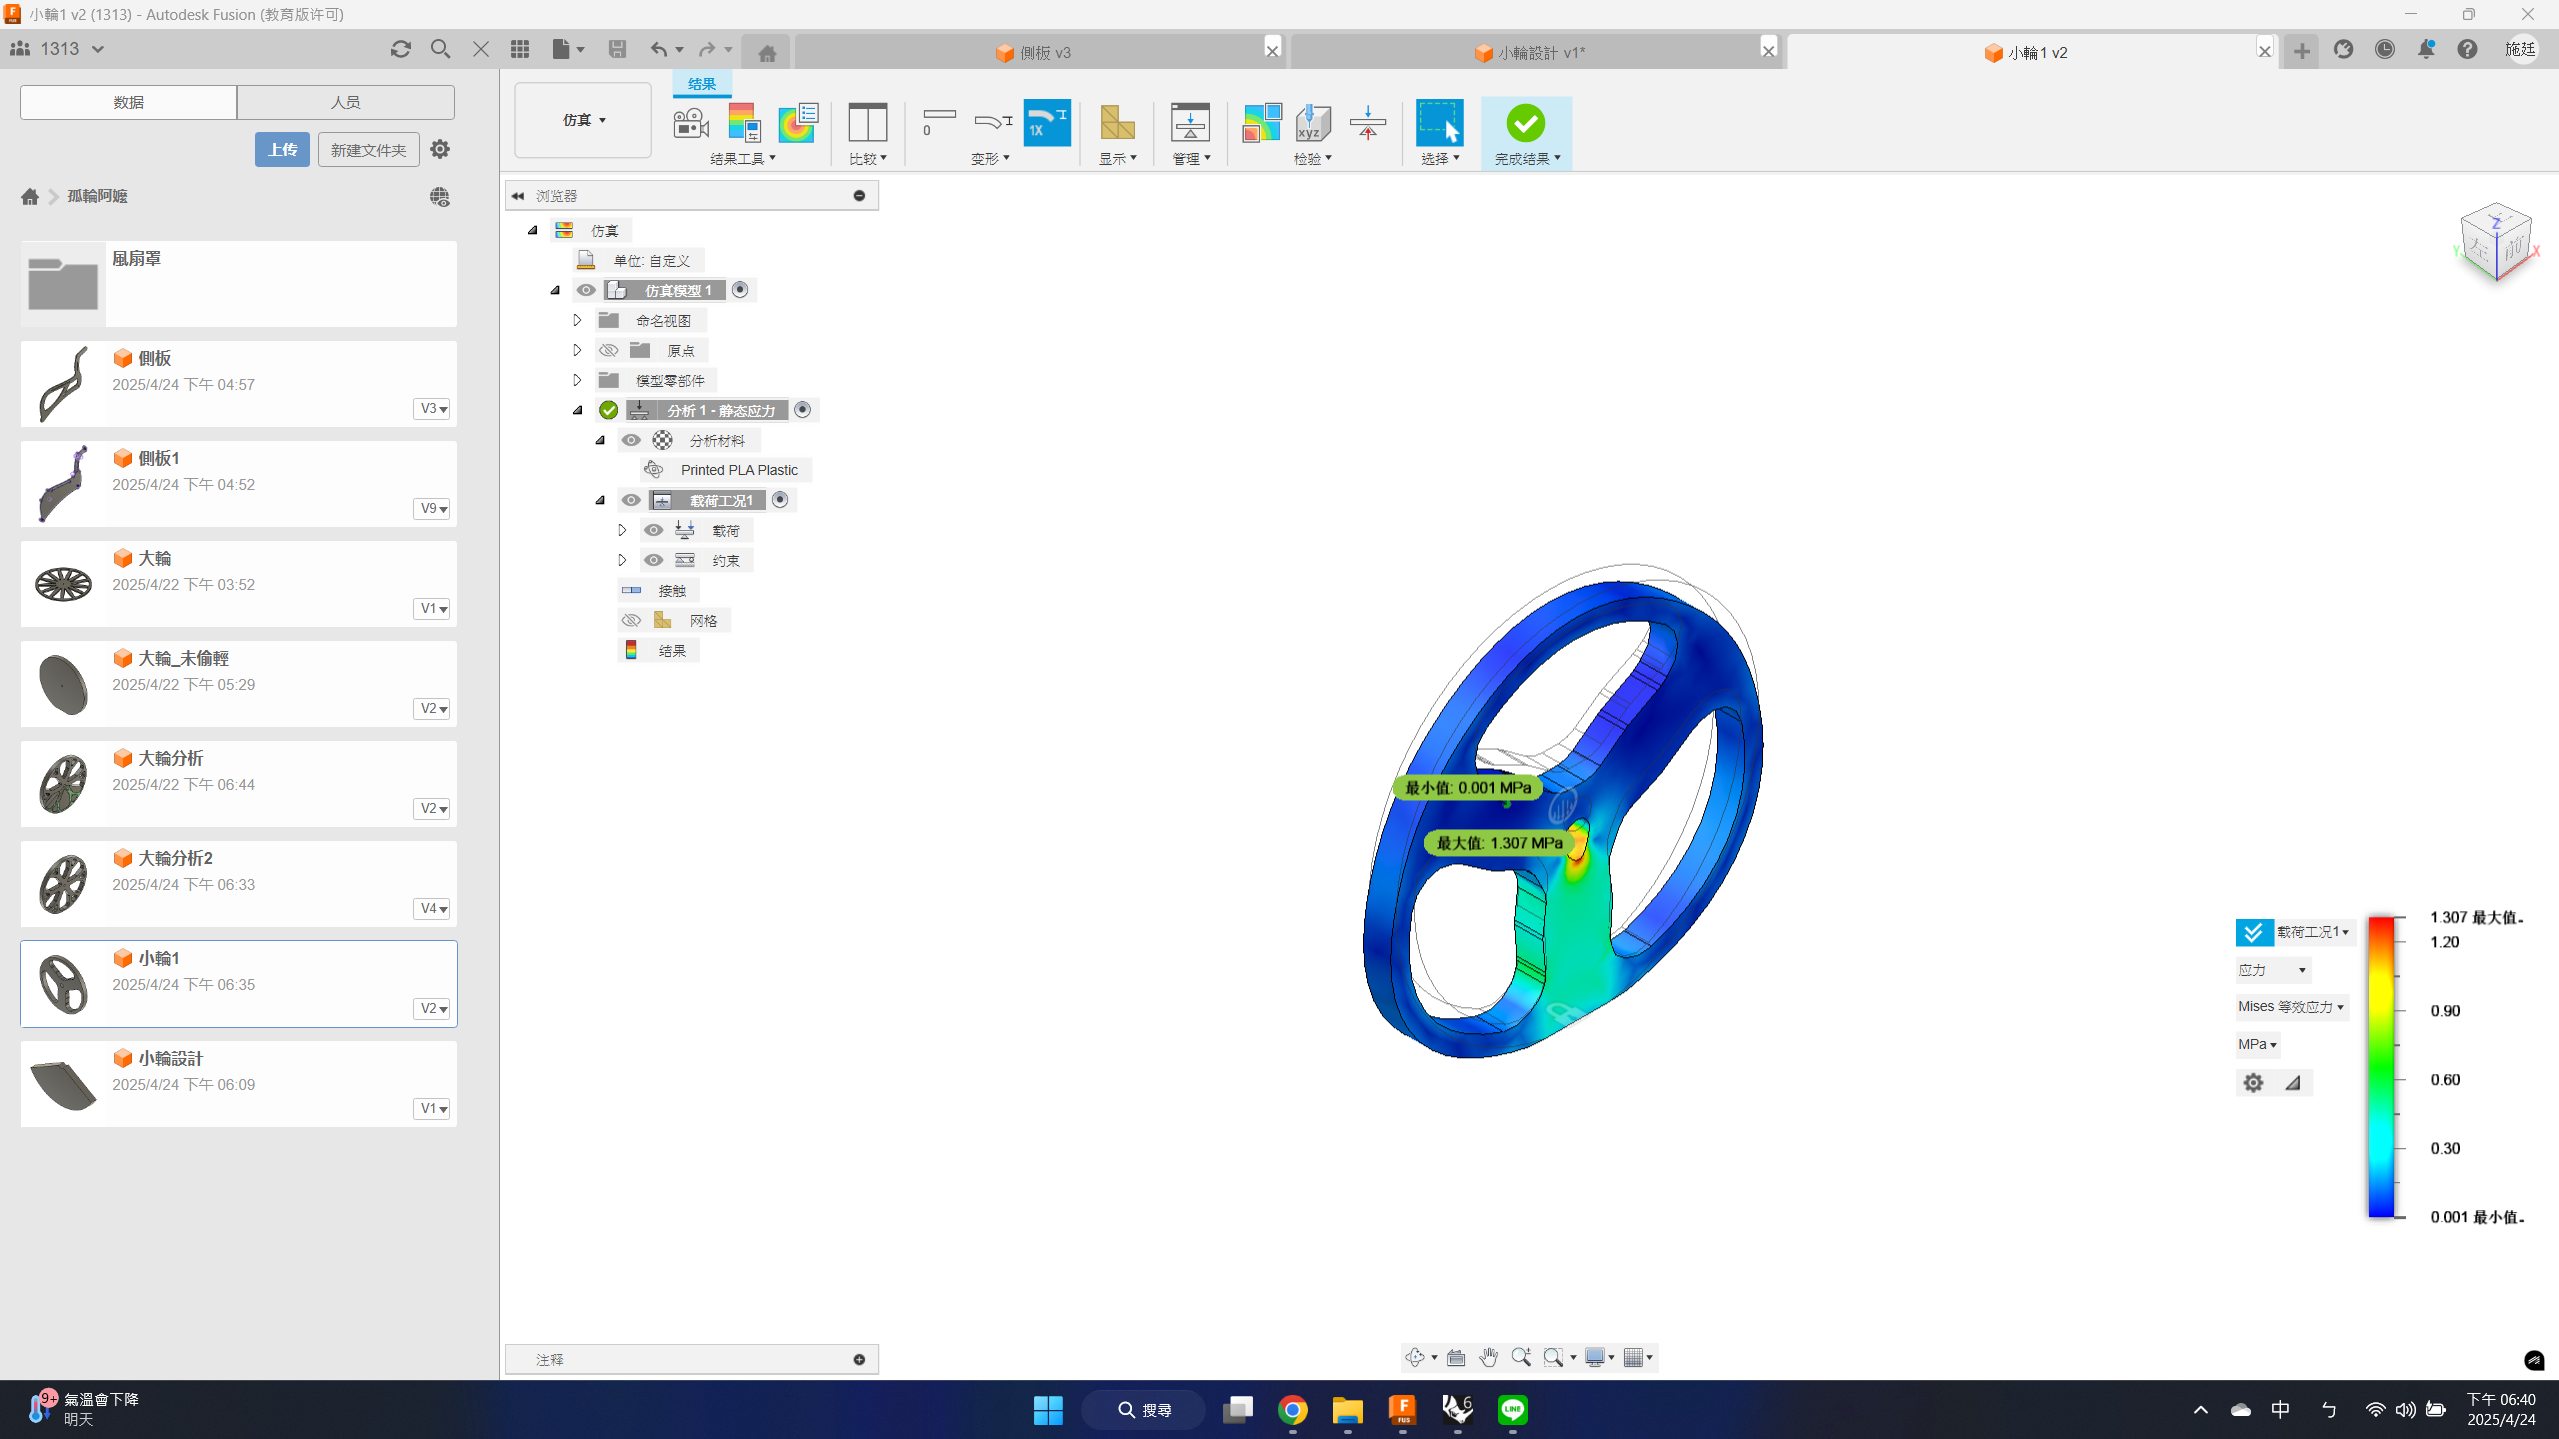
\includegraphics[width=0.7\textwidth]{54.jpg}     %圖片檔案名稱
    \caption{小輪的應力分析}    %圖片檔案名稱
    %如\ref{fig:example1}所示
\end{figure}

\begin{figure}[H]
    \centering
    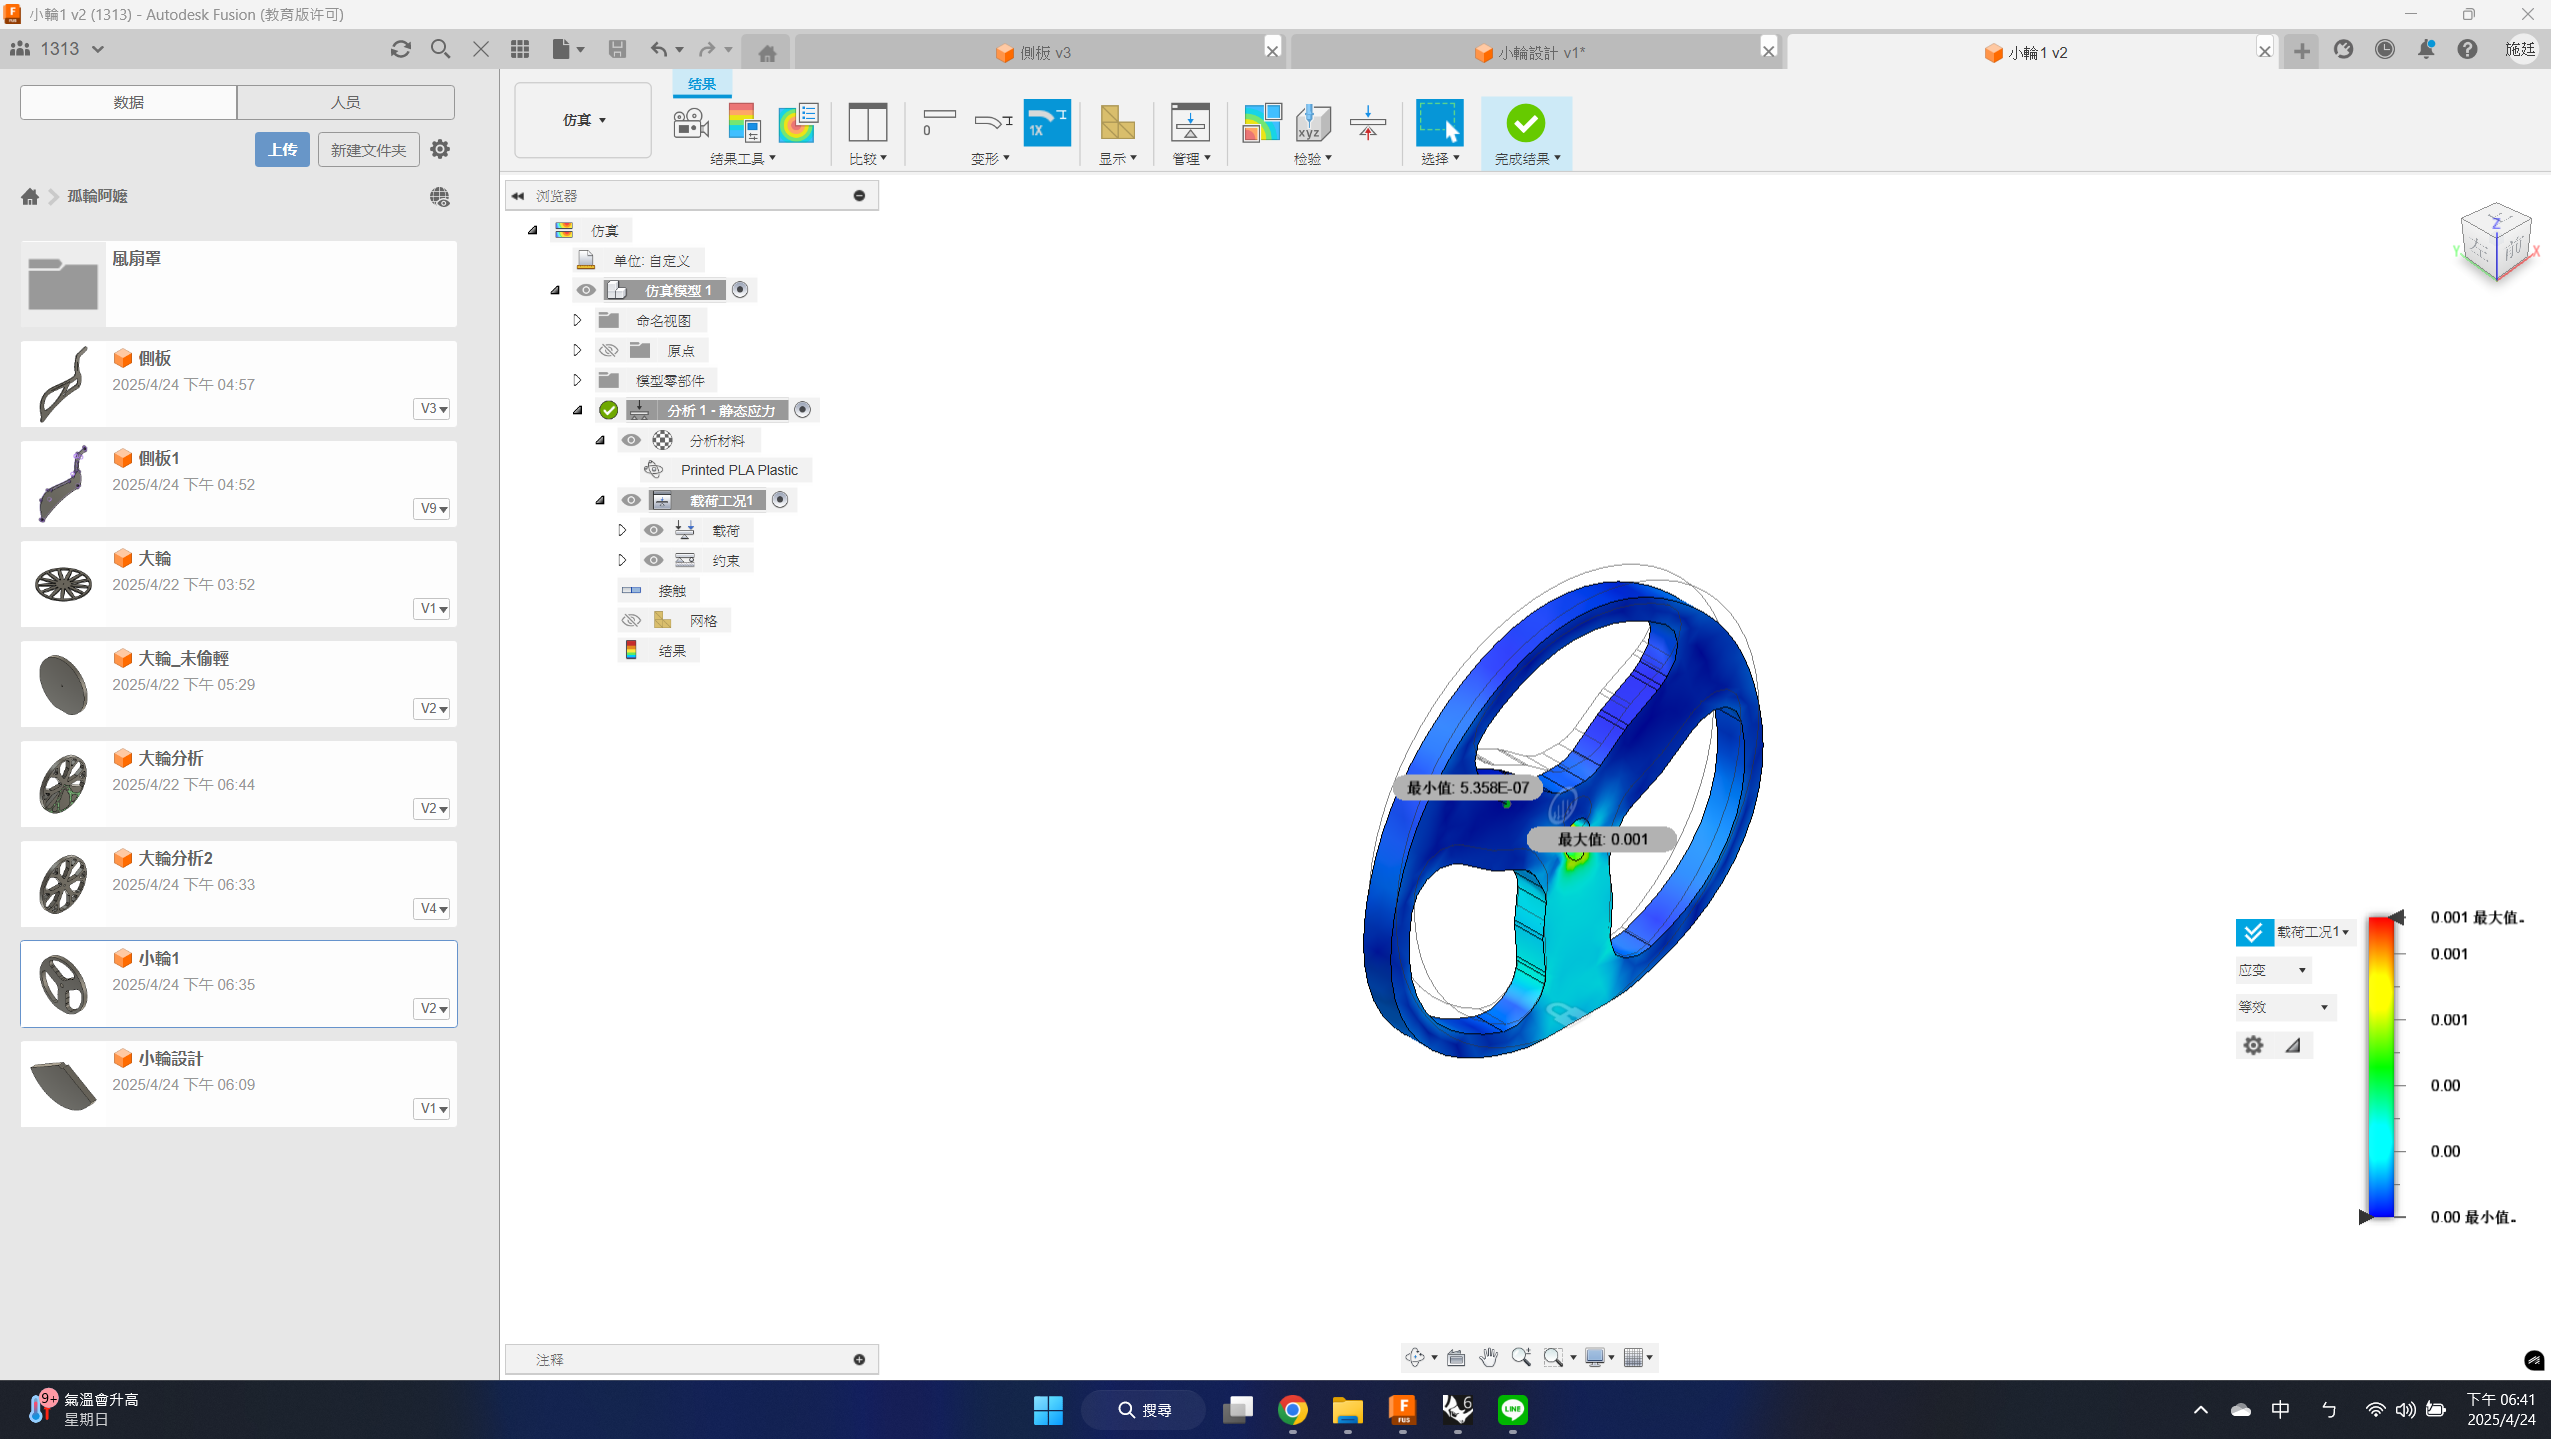
\includegraphics[width=0.7\textwidth]{55.jpg}     %圖片檔案名稱
    \caption{小輪的應變分析}    %圖片檔案名稱
    %如\ref{fig:example1}所示
    \label{fig:55}
\end{figure}
%==============================內文==============================


\section{\centering 製程與實作}
%==============================內文==============================
\hspace{2em}

%==============================內文==============================

\section{\centering 測試與驗證}

\subsection{風扇測試} 
%==============================內文==============================
\hspace{2em}以下是對風扇進行實際測試。
測試內容包含風扇開度對應理論風速(如圖\ref{fig:28}所示)、對應電流(如圖\ref{fig:29}所示)、
開度對應功率(如圖\ref{fig:30}所示)、對應推力(如圖\ref{fig:31}所示)與對應力效(如圖\ref{fig:32}所示)。

\begin{figure}[H]
    \centering
    
\includegraphics[width=0.7\textwidth]{28.jpg}     %圖片檔案名稱
    \caption{風扇開度對應理論風速曲線圖}    %圖片檔案名稱
    \label{fig:28}    %為圖片添加標籤
    %如\ref{fig:example1}所示
\end{figure}

\begin{figure}[H]
    \centering
    
\includegraphics[width=0.7\textwidth]{29.jpg}     %圖片檔案名稱
    \caption{風扇開度對應電流曲線圖}    %圖片檔案名稱
    \label{fig:29}    %為圖片添加標籤
    %如\ref{fig:example1}所示
\end{figure}

\begin{figure}[H]
    \centering
    
\includegraphics[width=0.7\textwidth]{28.jpg}     %圖片檔案名稱
    \caption{風扇開度對應功率曲線圖}    %圖片檔案名稱
    \label{fig:30}    %為圖片添加標籤
    %如\ref{fig:example1}所示
\end{figure}

\begin{figure}[H]
    \centering
    
\includegraphics[width=0.7\textwidth]{28.jpg}     %圖片檔案名稱
    \caption{風扇開度對應推力曲線圖}    %圖片檔案名稱
    \label{fig:31}    %為圖片添加標籤
    %如\ref{fig:example1}所示
\end{figure}

\begin{figure}[H]
    \centering
    
\includegraphics[width=0.7\textwidth]{28.jpg}     %圖片檔案名稱
    \caption{風扇開度對應力效曲線圖}    %圖片檔案名稱
    \label{fig:32}    %為圖片添加標籤
    %如\ref{fig:example1}所示
\end{figure}
%==============================內文==============================

\section{\centering 結論與反思}
%==============================內文==============================
\hspace{2em}


%==============================內文==============================




\section{\centering 參考文獻}
%==============================內文==============================
\renewcommand{\refname}{}  % 去除 "References" 標題
\printbibliography  % 列出參考文獻
%==============================內文==============================

\section{\centering 附錄}

\subsection{程式碼} 
%==============================內文==============================
\hspace{2em}影像偵測演算法以 Python 撰寫，報告則使用 LaTeX 系統進行編輯與排版；
所有原始程式碼均公開於王子晨的 GitHub 儲存庫，以利後續參考與驗證。網址如下：

https://github.com/PrinceLego/Practice\_Of\_Mechanical\_Engineering.git
%==============================內文==============================

\subsection{物料清單與發票收據} 
%==============================內文==============================
\hspace{2em}
\begin{figure}[H]
    \centering
    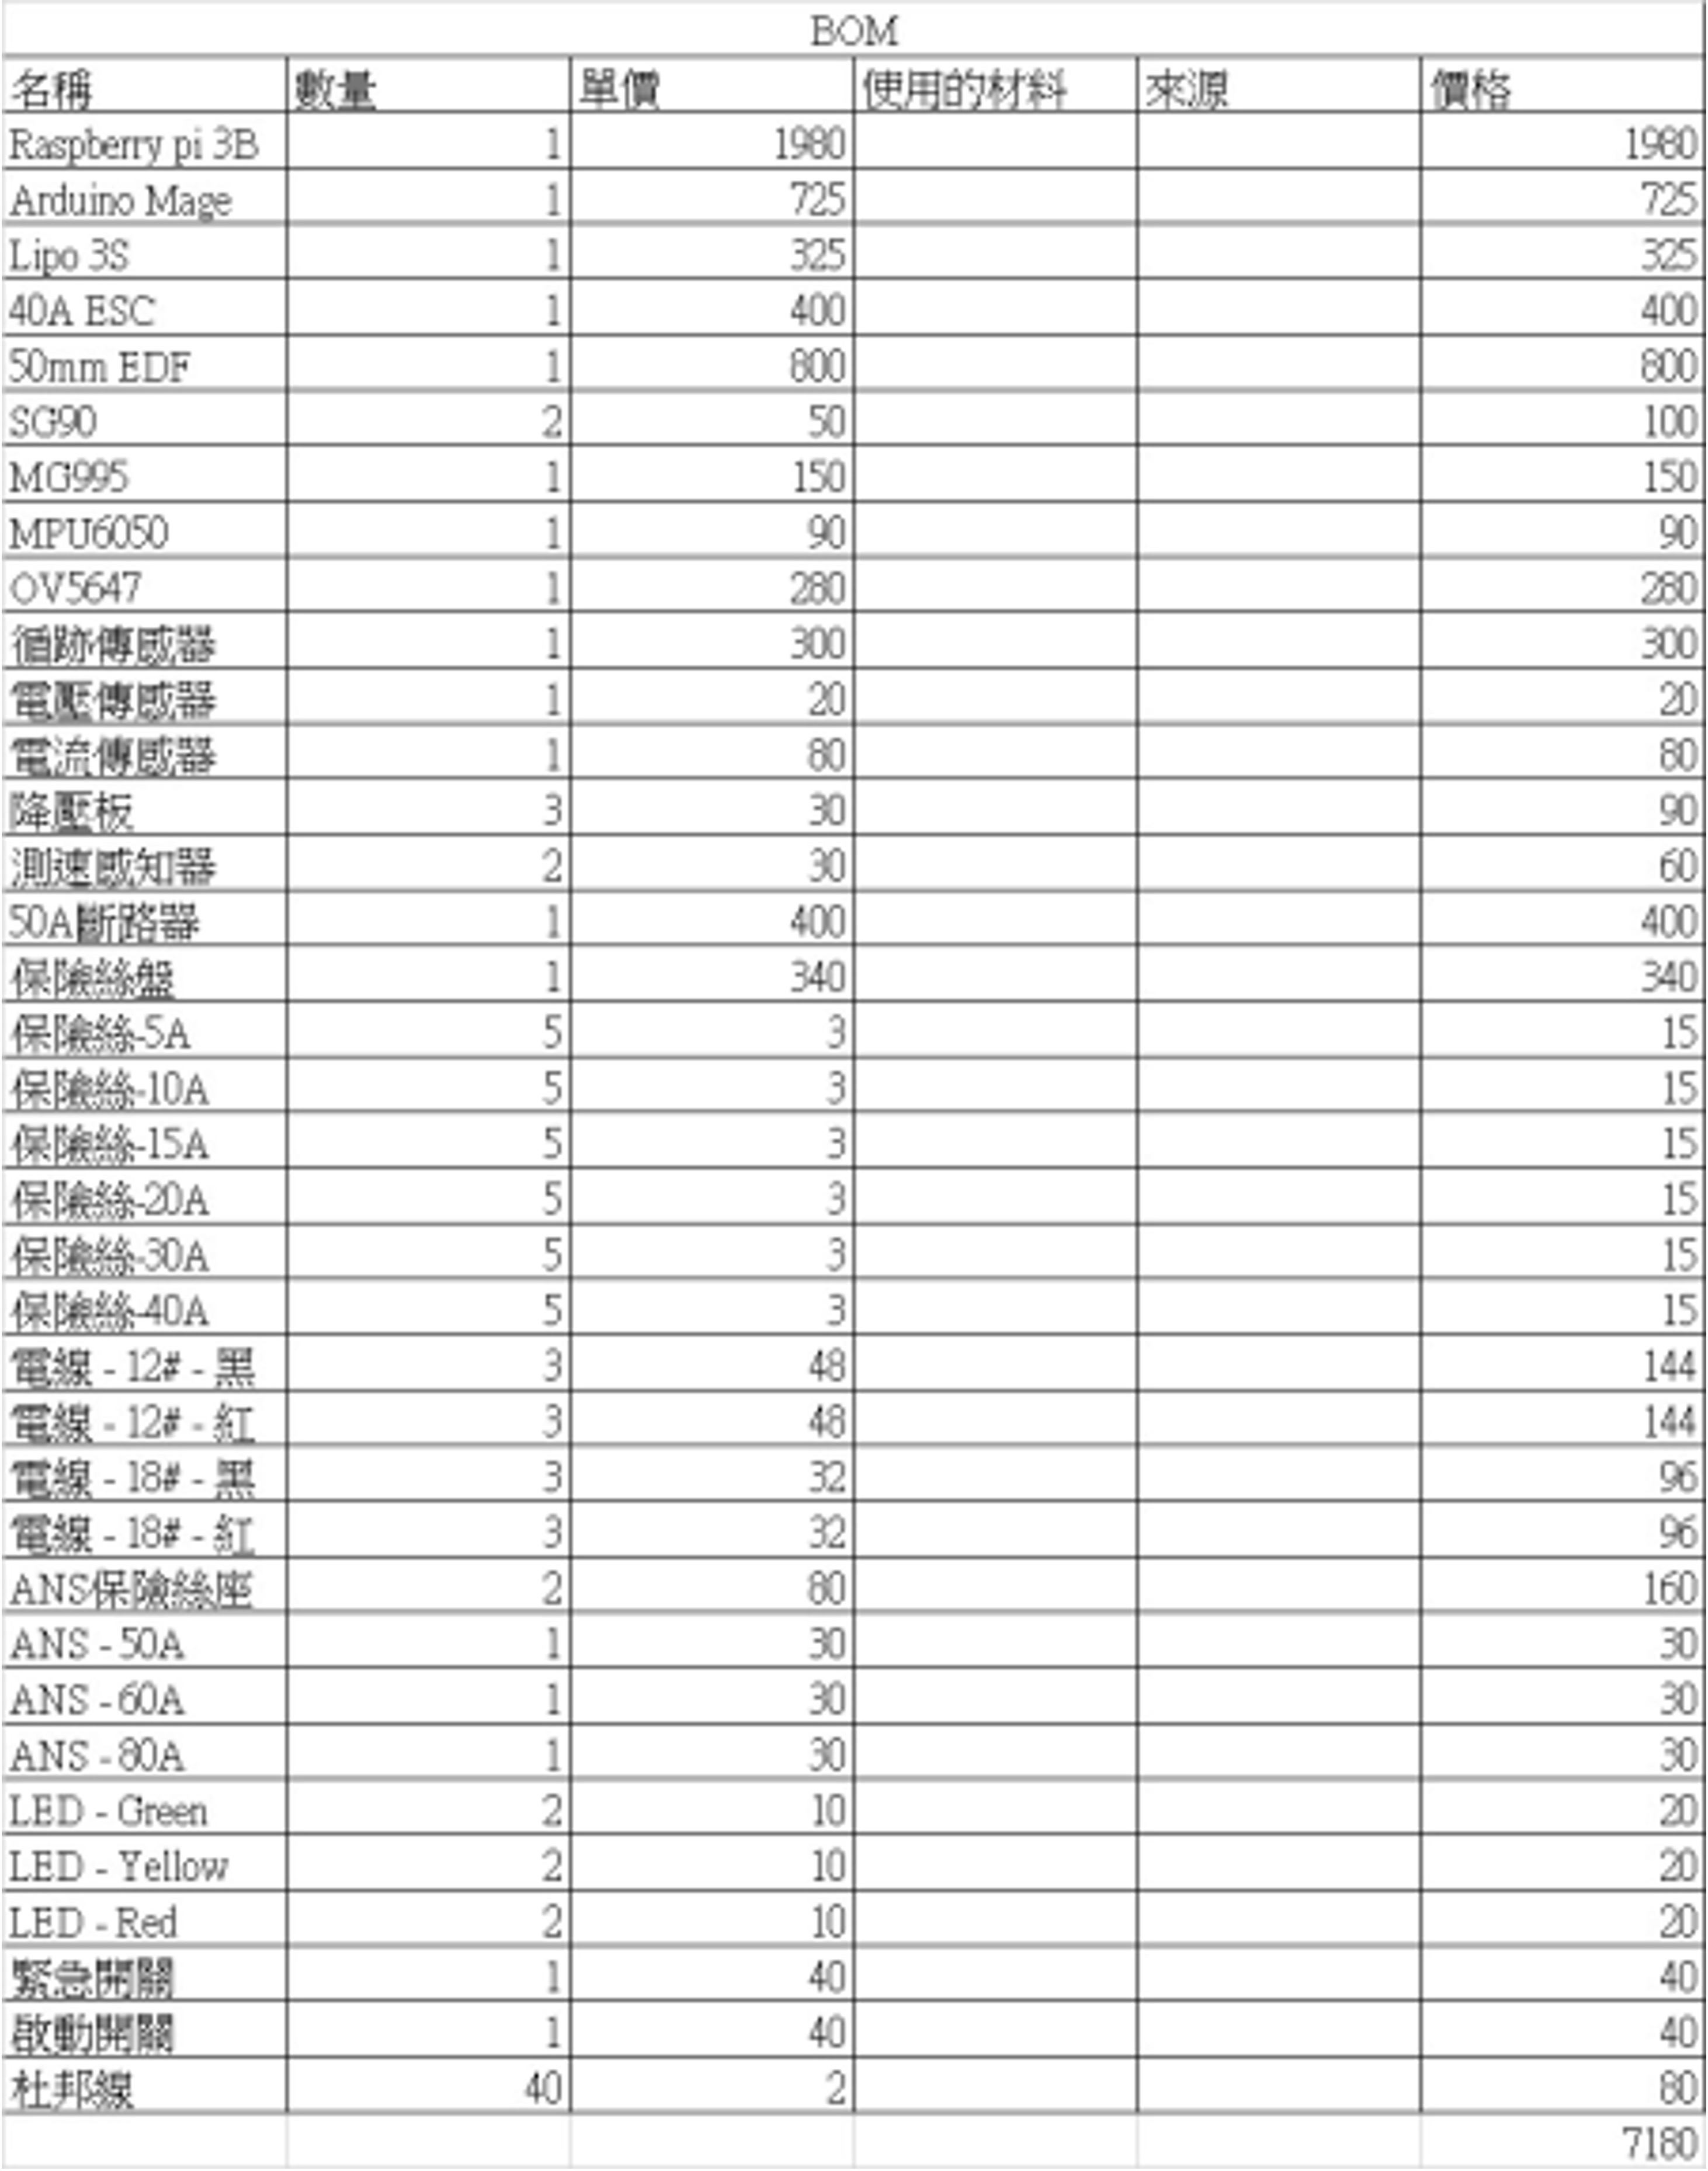
\includegraphics[width=0.7\textwidth]{8.jpg}     %圖片檔案名稱
    \caption{bom表}    %圖片檔案名稱
    \label{fig:8}    %為圖片添加標籤
    %如\ref{fig:example1}所示
\end{figure}
%==============================內文==============================


\end{document}

%=============================================================================================================================
%=============================================================================================================================
%=============================================================================================================================


\begin{comment}

\section{\centering 緒論}
\subsection{研究問題} 
\subsubsection{違規車輛偵測}
    
%==============================圖片==============================

\begin{figure}[H]
    \centering
    \includegraphics[width=0.7\textwidth]{截圖 2025-01-24 03.21.17.jpg}     %圖片檔案名稱
    \caption{這是圖片的標題}    %圖片檔案名稱
    \label{fig:example2}    %為圖片添加標籤
    %如\ref{fig:example1}所示
\end{figure}
    
%==============================數學公式==============================

\begin{align}
    a &= b + c \label{eq:1}
    \\
    d &= e - f \label{eq:2}
    %式\ref{eq:2}
\end{align}
    
%==============================表格==============================

\begin{table}[H]
    \centering
    \caption{致動器的功能與數目列表}
    \vspace{6pt} % 增加空格
    \label{tab:c}
    \begin{tabular}{lll}
        \toprule
        \textbf{項目} & \textbf{功能} & \textbf{數量}\\
        \midrule
        Wemos D1  & 接收個人電腦指令控制l298n &1\\
        ESP32-CAM  & 拍攝影像並傳輸至個人電腦 &1\\
        MacBook M1  & 影像偵測與控制演算法計算 &1\\
        l298n  & 麥克納姆輪 &2\\
        \bottomrule
    \end{tabular}
    %如\ref{tab:TT2}所示
\end{table}
    
\begin{table}[H]
    \centering
    \caption{C922 Pro Stream 規格}
    \vspace{6pt} % 增加空格
    \label{tab:C922 Pro}
    \begin{tabular}{ll}
        \toprule
        \textbf{項目} & \textbf{規格} \\
        \midrule
        解析度  & 1280$\times$720 (HD) \\
        幀率  & 30fps \\
        水平視角 & 70.42$^\circ$ \\
        垂直視角  & 43.3$^\circ$ \\
        \bottomrule
    \end{tabular}
\end{table}

%==============================條列==============================

%無序條列

\begin{itemize}
    \item 第一項
    \item 第二項
    \item 第三項
\end{itemize}

%有序條列

\begin{enumerate}
    \item 第一項
    \item 第二項
    \item 第三項
\end{enumerate}

    \end{comment}
        